%% File encoding: UTF-8
%% äöüÄÖÜß  <-- keine deutschen Umlaute hier? UTF-faehigen Editor verwenden!

\documentclass[master,english]{hgbthesis}
% Zulässige Class Options: 
%   Typ der Arbeit: diplom, master (default), bachelor, praktikum 
%   Hauptsprache: german (default), english
%%------------------------------------------------------------

\RequirePackage[utf8]{inputenc}		% remove when using lualatex oder xelatex!

\graphicspath{{images/}}    % name of directory containing the images
\logofile{logo}							% name of logo-PDF in images/ (or use \logofile{} for no logo)
\bibliography{literature}  	% name of the BibTeX (.bib) file


%%%----------------------------------------------------------
\begin{document}
%%%----------------------------------------------------------

% Einträge für ALLE Arbeiten: --------------------------------
\title{Mobile Device Usage in Interactive, Co-located Presentations}
\author{Iris M.\ Schaffer}
\studiengang{Interactive Media}
\studienort{Hagenberg}
\abgabedatum{2016}{09}{26}	% {YYYY}{MM}{DD}

%%%----------------------------------------------------------
\frontmatter
\maketitle
\tableofcontents
%%%----------------------------------------------------------

%\chapter{Vorwort} 	% engl. Preface


Dies ist \textbf{Version \hgbthesisDate} der \latex-Dokumentenvorlage für 
verschiedene Abschlussarbeiten an der Fakultät für Informatik, Kommunikation
und Medien der FH Oberösterreich in Hagenberg, die mittlerweile auch 
an anderen Hochschulen im In- und Ausland gerne verwendet wird.

Das Dokument entstand ursprünglich auf Anfragen von Studierenden,
nachdem im Studienjahr 2000/01 erstmals ein offizieller
\latex-Grundkurs im Studiengang Medientechnik und -design an der
FH Hagenberg angeboten wurde. Eigentlich war die Idee, die bereits
bestehende \emph{Word}-Vorlage für Diplomarbeiten "`einfach"' in
\latex\ zu übersetzen und dazu eventuell einige spezielle
Ergänzungen einzubauen. Das erwies sich rasch als wenig
zielführend, da \latex, \va was den Umgang mit Literatur und
Grafiken anbelangt, doch eine wesentlich andere Arbeitsweise
verlangt. Das Ergebnis ist -- von Grund auf neu geschrieben und
wesentlich umfangreicher als das vorherige Dokument --
letztendlich eine Anleitung für das Schreiben mit \latex, ergänzt
mit einigen speziellen (mittlerweile entfernten) Hinweisen für \emph{Word}-Benutzer.
Technische Details zur aktuellen Version finden sich in Anhang \ref{ch:TechnischeInfos}.

Während dieses Dokument anfangs ausschließlich für die Erstellung
von Diplomarbeiten gedacht war, sind nunmehr auch  
\emph{Masterarbeiten}, \emph{Bachelor\-arbeiten} und \emph{Praktikumsberichte} 
abgedeckt, wobei die Unterschiede bewusst gering gehalten wurden.

Bei der Zusammenstellung dieser Vorlage wurde versucht, mit der
Basisfunktionalität von \latex das Auslangen zu finden und -- soweit möglich --
auf zusätzliche Pakete zu verzichten. Das ist nur zum Teil gelungen;
tat\-säch\-lich ist eine Reihe von ergänzenden "`Paketen"' notwendig, wobei jedoch
nur auf gängige Erweiterungen zurückgegriffen wurde.
Selbstverständlich gibt es darüber hinaus eine Vielzahl weiterer Pakete,
die für weitere Verbesserungen und Finessen nützlich sein können. Damit kann
sich aber jeder selbst beschäftigen, sobald das notwendige Selbstvertrauen und
genügend Zeit zum Experimentieren vorhanden sind.
Eine Vielzahl von Details und Tricks sind zwar in diesem Dokument nicht explizit
angeführt, können aber im zugehörigen Quelltext jederzeit ausgeforscht
werden.

Zahlreiche KollegInnen haben durch sorgfältiges Korrekturlesen und
konstruktive Verbesserungsvorschläge wertvolle Unterstützung
geliefert. Speziell bedanken möchte ich mich bei Heinz Dobler für
die konsequente Verbesserung meines "`Computer Slangs"', bei
Elisabeth Mitterbauer für das bewährte orthographische Auge und
bei Wolfgang Hochleitner für die Tests unter Mac~OS.

Die Verwendung dieser Vorlage ist jedermann freigestellt und an
keinerlei Erwähnung gebunden. Allerdings -- wer sie als Grundlage
seiner eigenen Arbeit verwenden möchte, sollte nicht einfach
("`ung'schaut"') darauf los werken, sondern zumindest die
wichtigsten Teile des Dokuments \emph{lesen} und nach Möglichkeit
auch beherzigen. Die Erfahrung zeigt, dass dies die Qualität der
Ergebnisse deutlich zu steigern vermag.

Der Quelltext zu diesem Dokument sowie das zugehörige
\latex-Paket sind in der jeweils aktuellen Version online
verfügbar unter
%
\begin{itemize}
\item[]\url{https://sourceforge.net/projects/hgbthesis/}.
\end{itemize}
%
Trotz großer Mühe enthält dieses Dokument zweifellos Fehler und Unzulänglichkeiten
-- Kommentare, Verbesserungsvorschläge und passende Ergänzungen
sind daher stets willkommen, am einfachsten per E-Mail direkt an mich:
\begin{itemize}
\item[]%

Dr.\ Wilhelm Burger, Department für Digitale Medien,\newline
Fachhochschule Oberösterreich, Campus Hagenberg (Österreich)\newline
\nolinkurl{wilhelm.burger@fh-hagenberg.at}
\end{itemize}

\noindent
Übrigens, hier im Vorwort (das bei Diplom- und Masterarbeiten üblich, bei Bachelorarbeiten 
aber entbehrlich ist) kann kurz auf die Entstehung des Dokuments eingegangen werden.
Hier ist auch der Platz für allfällige Danksagungen (\zB an den Betreuer, 
den Begutachter, die Familie, den Hund, \ldots), Widmungen und philosophische 
Anmerkungen. Das sollte allerdings auch nicht übertrieben werden und sich auf 
einen Umfang von maximal zwei Seiten beschränken.




		% ggfs. weglassen
%
%
\chapter{Kurzfassung}

An dieser Stelle steht eine Zusammenfassung der Arbeit, Umfang
max.\ 1 Seite. Im Unterschied zu anderen Kapiteln ist die
Kurzfassung (und das Abstract) üblicherweise nicht in Abschnitte
und Unterabschnitte gegliedert. 
Auch Fußnoten sind hier falsch am Platz.

Kurzfassungen werden übrigens häufig -- zusammen mit Autor und Titel
der Arbeit -- %
in Literaturdatenbanken aufgenommen. Es ist daher darauf zu
achten, dass die Information in der Kurzfassung für sich 
\emph{allein} (\dah ohne weitere Teile der Arbeit) zusammenhängend und
abgeschlossen ist. Insbesondere werden an dieser Stelle (wie \ua
auch im \emph{Titel} der Arbeit und im \emph{Abstract})
normalerweise \emph{keine Literaturverweise} verwendet! Falls
unbedingt solche benötigt werden -- etwa weil die Arbeit eine
Weiterentwicklung einer bestimmten, früheren Arbeit darstellt --,
dann sind \emph{vollständige} Quellenangaben in der Kurzfassung
selbst notwendig, \zB %
[\textsc{Zobel} J.: \textit{Writing for Computer Science -- The Art of
Effective Commu\-nica\-tion}. Springer-Verlag, Singa\-pur, 1997].

Weiters sollte daran gedacht werden, dass bei der Aufnahme in Datenbanken
Sonderzeichen oder etwa Aufzählungen mit "`Knödellisten"' in der
Regel verloren gehen. Dasselbe gilt natürlich auch für das 
\emph{Abstract}.


Inhaltlich sollte die Kurzfassung \emph{keine} Auflistung der
einzelnen Kapitel sein (dafür ist das Einleitungskapitel
vorgesehen), sondern dem Leser einen kompakten, inhaltlichen
Überblick über die gesamte Arbeit verschaffen. Der hier verwendete
Aufbau ist daher zwangsläufig anders als der in der Einleitung.
		
%
%\chapter{Abstract}
Mobile devices such as smartphones, tablets and laptops have become our every day companions and can act as an endless source of information, knowledge and inspiration. However, despite studies having demonstrated the benefits of targeted smartphone use in classrooms and meetings, they are still perceived as impolite and disturbing during presentations. These, on the other hand, are often still one-man endeavours, from slide preparation, giving the talk to lastly follow-up work such as hand-outs. In an effort to destigmatise mobile devices usage and make presentations more memorable, engaging, and collaborative, a prototype of an extensible JavaScript presentation eco\-system with a multitude of interactive mechanisms was implemented. These functionalities are the result of the analysis of several types of presentations and their weaknesses and, amongst others, include the possibility for the audience to browse and follow slides on any mobile device to account for individual learning-pace, as well as spontaneous reactions via emoji and votes on polls (both prepared and created on-the-fly) to more reliably estimate ones crowd's mood and background knowledge. Moreover, to truely involve audience memers in shaping the presentation, the functionality to alter the $2$-dimensional slide-sets in real time was realised. This way, listeners can share related multi-media content as well as questions and comments as new main or sub-slides.

Although more thorough, long-term studies will be necessary to validate our approach, consequent informal evaluation of the system in internal presentations and meetings has been promising and decidedly positive. Despite showing room for improvement, all features were understood by the users, with the content sharing functionality sparking most interest and excitement among listeners. The observation of the usage of the tool has moreover given way to further research projects and ideas. 			
%

%%%----------------------------------------------------------
\mainmatter         % Hauptteil (ab hier arab. Seitenzahlen)
%%%----------------------------------------------------------

\chapter{Introduction}
\label{cha:introduction}

\section{Motivation}

Mobile phones, tablets and laptops have become our every day companions. We take them with us wherever we go, may it be the classroom or meetings, lately they have even made an appearance in courtrooms \cite{Farrell:TrialByTablet}. Especially during presentations mobile device usage is still perceived as impolite and can be a source of distraction \cite{Bohmer:SmartphoneUseRude, Bajko:ComparativePerceptionSmartphoneMeeting, Kuznekoff:ImpactPhoneStudentLearning}, although studies indicate that lecture-relevant phone use in classrooms can actually be beneficial for information-recall \cite{Kuznekoff:MobilePhoneClassroomTwitter}.

Presentations, on the other hand, have remained largely unchanged since the launch of PowerPoint in the late 1980s \cite{Yates:PowerPoint}. In fact, some of the features overhead projectors innately offered, namely the annotation of transparencies during the presentation and sorting and choosing slides before presenting them, have effectively been lost with the introduction of presentation software. While the amount of presentations given has continuously risen, the modus of presenting has stayed untouched: In most cases, there is one presenter and a group of co-located listeners. The speaker prepares slides prior to a presentation and has the responsibility of educating, fascinating, inspiring and keeping the audience awake, while catering the presented contents to the respective listeners. Although interactive elements in presentations have proven to be twice as effective at engaging listeners and beneficial to information-recall \cite{prezi-science}, presentations have largely remained a static endeavor for the speaker alone.

Mobile phones, tablets and laptops, however, hold the potential of challenging this status quo. Their growing computing power as well as ubiquitousness make them suitable candidates for interacting with presentation software, thus transforming presentations into a more collaborative effort. Instead of banning modern technologies, incorporating mobile devices has proven to foster collaboration and connection between attendees in meetings \cite{Bohmer:SmartphoneUseRude} and has the potential of promoting participation and helping introverts overcome the hurdle of speaking out loud \cite{Bry:Backstage}. At the core of this thesis therefore stands the question: How can mobile devices be integrated into presentation workflows to engage and involve the audience, while transforming the stigma around mobile phones into something positive?

\section{Goals}

\begin{figure}
\centering
\includegraphics[width=.8\textwidth]{illustrations/meeting}
\caption{Unveil presentation in action: the projector displays the current slide, listeners can follow and interact with presentations on their personal devices and listeners can control the presentation using theirs.}
\label{fig:introduction-meeting}
\end{figure}

The main objective of the project consequently is the exploration of different ways of incorporating personal devices in presentations efficiently and productively. This involves both the conception of such mechanisms, as well as their implementation in an online presentation tool.
Due to the high number of different settings and contexts in which talks can be given, and since we feel meetings and other business-related presentations with small numbers of attendees offer the perfect playground and most possibilities for interactive mechanisms, this thesis focuses on presentations in business-settings.

The proposed presentation software includes device-independent altering of pre-defined $2$-dimensional slide-sets by listeners and presenters in real time. It allows audience members to view slides on their personal devices, either navigating freely or synchronised with the presenter (see figure \ref{fig:introduction-meeting}). Additionally, the developed libraries offer support for real-time voting, as well as voting creation on-the-fly. Instantaneous audience reactions via emoji and different paths through the presentation were also realised.

As far as the implementation is concerned, it was our declared goal to create a modular ecosystem other developers can tap into, reuse, overwrite and extend. Since the web was chosen as a platform for its rapid prototyping and iteration cylce possibilities, it was paramount to make the application feel as fast and responsive as possible, to give it the look and feel of a native application \cite{Charland:WebVsNative}. Therefore the user interface and interaction design were at the core of the project with the overall objective of creating an interface that works across all devices, without feeling unnatural.

Finally, an evaluation of the developed mechanisms was desirable. Since thorough long-term studies with control groups are beyond the scope of a master thesis, we constrained ourselves to the informal observation of the system in a series of internal meetings and presentations.

\section{Structure}

This thesis is organised into eight main chapters. First of all, we want to establish the context around the present work by introducing the reader to existing research and projects in the field of interactive presentations in chapter \ref{cha:related-work}. Since an overwhelming number of studies have been conducted in educational settings, the chapter is further divided into classroom \ref{sec:related-work-classroom} and office \ref{sec:related-work-office} related approaches as well as general presentations \ref{sec:related-work-general}.

In chapter \ref{cha:mechanisms} different types of presentations are analysed for their shortcomings and suitable solutions are developed. These are formulated into distinct interactive mechanisms for which clear requirements are established.
Based on these requirements, chapter \ref{cha:design} goes into details on the interface and interaction design of the application as a whole and each of its interactive mechanisms. The general flow and setup of the proposed software are also discussed.

Chapter \ref{cha:implementation} lays out the entire implementation of the libraries involved in the presentation tool. It first defines the scope of the project \ref{sec:implementation-scope} to then cover the server setup \ref{sec:implementation-server}, before offering more insight into the underlying front end technologies used \ref{sec:implementation-technologies}. Finally the general project structure \ref{sec:implementation-structure}, as well as all developed libraries are discussed in detail.

Since we pride ourselves in having developed an entirely open-sourced presentation ecosystem which we want others to explore, reuse and extend, chapter \ref{cha:results} shortly addresses the usage of the resulting libraries from a developer's perspective.

Chapter \ref{cha:discussion} outlines the results of our informal evaluation and observation of the system in regards to its usability \ref{sec:discussion-usability} and the creation of presentations \ref{sec:discussion-dev}, to then reflect on the chosen architecture \ref{sec:discussion-architecture} and give an outlook on future work \ref{sec:discussion-future-work}.

Finally, we briefly talk about the conclusions we draw from this project in chapter \ref{cha:conclusion} and again summarise our findings.
\chapter{Related Work}
\label{cha:related-work}

Mobile phones, tablets and laptops have become our every day companions. We take them with us wherever we go, may it be the classroom or meetings, lately they have even made an appearance in courtrooms \cite{Farrell:TrialByTablet}. Especially during presentations, mobile device usage is still perceived as rude and can be a source of distraction \cite{Bohmer:SmartphoneUseRude, Bajko:ComparativePerceptionSmartphoneMeeting, Kuznekoff:ImpactPhoneStudentLearning} although other studies indicate that lecture-relevant phone use in classrooms can actually be beneficial \cite{Kuznekoff:MobilePhoneClassroomTwitter} for information-recall.

Instead of banning modern technologies, incorporating mobile devices into presentation workflows has proven to foster collaboration and connection between attendees in meetings \cite{Bohmer:SmartphoneUseRude} and holds the potential of promoting participation and helping introverts overcome the hurdle of speaking out loud \cite{Bry:Backstage}. The growing computing power as well as the ubiquitousness of mobile phones, tablets and laptops make them suitable candidates for giving instant feedback to speakers as well as voting and sharing relevant multi-media content on-the-fly. Resulting presentations provide more flexibility, a better understanding of the listeners' opinion and the possibility to close the gap between presenter and audience.

The idea of using electronic devices to foster group interaction in meetings and presentations is not new. Stefik et al. \cite{Stefik:BeyondTheChalkboard} already experimented with the use of personal computers in meeting rooms as early as 1987 and Myers et al. \cite{Myers:CollaborationPDAs} developed a collaboration tool which could be used to annotate PowerPoint slides from PDAs in 1998. Since then, digital whiteboards, telepresence systems, productive multi-user web applications and other computer-aided collaboration tools have become a common sight and we choose to carry smart devices around wherever we go. Surprisingly little research, however, has covered the use of these mobile devices in the context of presentations. Most of these studies were conducted in the educational sector and usually aim at quizzing students, which is why an own sub section is dedicated to classroom related approaches. 

\section{Classroom related}

\begin{figure}
\centering
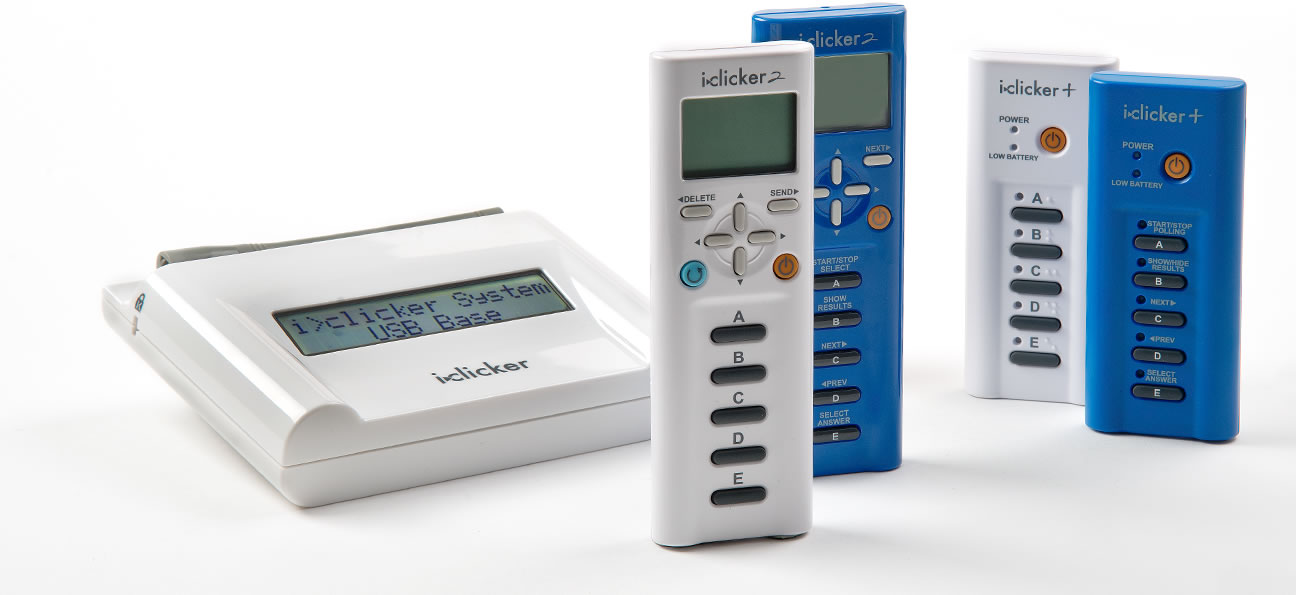
\includegraphics[width=.65\textwidth]{iclickers}
\caption{\emph{i>clicker} devices, used in \cite{Chamillard:StudentResponseSystem}. Image source \cite{iclicker}.}
\label{fig:related-work-iclicker}
\end{figure}

As growing class-sizes have caused student participation to sink drastically \cite{Bry:Backstage}, researchers have tried to deploy mechanisms to make lectures more interactive and engaging. The first ap\-proa\-ches in this field of student-response-systems (SRS) utilised so-called clickers (see figure \ref{fig:related-work-iclicker}) -- remote-control-like devices, connected to a receiver station via radio frequency technology \cite{cuclickers:faq} which can be used for tasks like taking attendance and voting \cite{Chamillard:StudentResponseSystem}. Using these clicker systems has shown to ``yield a strong and positive relationship with student learning'' \cite{Chamillard:StudentResponseSystem}. However, the limitations of clickers -- the need for proprietary hardware and the limited interface consisting only of a few buttons -- lead researchers to experiment with personal mobile devices as input instead. In 2007 Lindquist et al. \cite{Lindquist:ExploringMobilePhonesActiveLearning} presented a system integrated with the University of Washington's Classroom Presenter software, which lets students submit answers to assignments and in-class quizzes via SMS and MMS or using their laptops. Although the mobile phone users struggled with the input of longer messages, they perceived the ubiquity and concenience of using a light-weight personal device as an advantage. Most students, however, were worried about the costs of using SMS or MMS as a requirement in class -- a concern modern devices with internet access and cheap data plans dispel. The first of these web-based approaches were explored around the same time. Esponda \cite{Esponda:ElectronicVotingOnTheFly} for example describes a system in which iPods and other devices with access to wifi can be used to answer questions during class. What is interesting about her approach is not only the technology used, but also that questions do not have to be prepared in advance, but can also be created on-the-fly, using a pen-based tablet, resulting in more lively and spontaneous student-teacher-interaction.
The creators behind \emph{i>clicker}\footnote{\url{http://www1.iclicker.com/}}, the clicker system used in \cite{Chamillard:StudentResponseSystem}, have also recognised the shortcommings of their hardware-approach and now build mobile apps for students' personal devices. Like\cite{Esponda:ElectronicVotingOnTheFly}, their application makes it possible for lecturers to prepare quizzes beforehands or create polls on-the-fly to monitoring the students' knowledge, understanding and progress. Although also available as iOS and Android app, like most modern approaches, the i>clicker software also has a web version, making use of modern browsers' possibilities and the device-independence of the web as a platform.
The tool \emph{ASQ} \cite{Triglianos:InteractiveWebPresentationsImpress} for example lets lecturers create HTML5 presentations with \emph{impress.js}\footnote{\url{http://impress.github.io/impress.js}} which are then distributed to listeners via a link. Students follow the presentations on their mobile devices, and can submit questions connected to the current slide to the speaker. Quizzes (both open questions and multiple-choice) can be embedded in the slides by the teacher. These quizzes can either be graded automatically (for coding assignments and multiple-choice questions), corrected by teaching assistants or by the students in self or peer-assessment. While this project has put a lot of effort into the server-side and administration of slidesets, the present work concentrates more on the client-side and does not provide management tools. However, as noted by Esponda \cite{Esponda:ElectronicVotingOnTheFly}, being familiar with the listeners' understanding of a subject is important for creating the polls, which is why we also added the possibility to create votings spontaniously.
Another interesting approach is presented by Cheng et al. \cite{Cheng:TreebasedOnlinePresentations}, who propose a system which generates HTML presentations from \emph{Microsoft PowerPoint} slides and lets viewers add their own content (either additional material or questions) as vertical sub-slides. This way a tree-like structure is created in which teachers and students collaborate in interactive presentations. This architecture also inspired the sub-slide based presentation space deployed in this software.

Another popular application, with richer audience-spea\-ker-in\-ter\-ac\-tion and an emphasis on listener-listener-interaction is \emph{Backstage}\footnote{\url{http://backstage.pms.ifi.lmu.de/}}. As digital backchannels like Twitter can foster the sense of community within the audience, but are usually hard to follow for presenters, Bry et al.\cite{Bry:Backstage} developed a backchannel specifically for large classrooms. Students can post messages publicly and send private messages to their colleagues. These public posts can be up or down-voted, as well as marked as unrelated. Together with an ageing-algorithm, this community feedback is used to estimate a post's relevance. Important feedback is then presented to the lecturer, to allow him or her to get a better sense for the audiences' opinion and understanding. Additionally, small quizzes and polls serve as performance feedback to the teacher and students. Though one of the most mature systems studied for this thesis, having been developed specifically for classrooms, the use of the software in other scenarios is not ideal. Moreover, most of the features concentrate on listener-listener-interaction, while the present thesis focuses on mechanisms strengthening the speaker-audience-interaction.

\section{Office environments}

In contrast to classroom-related software, meeting-en\-vi\-ron\-ments usually have an significantly lower amount of participants, as well as a smaller gap between the speaker and the audience. Another difference lies in the polling, surveying and quizzing functionality most of the presented projects offer: while these usually have only one correct answer in educational settings, to grade students \cite{Lindquist:ExploringMobilePhonesActiveLearning, Triglianos:InteractiveWebPresentationsImpress, Bry:Backstage}, the goal in meeting environments is to make decisions and collect ideas, without judgment and often anonymously.
The chosen systems all have a focus on mobile devices and their usage in meetings and office-related presentations and were developed by Microsoft Research: In \cite{Bohmer:SmartphoneUseRude}, as well as examining the perception of smartphone use in meetings, the mobile application \emph{Meetster} is presented. The study finds that although people primarily use their phones for meeting or work-related tasks, they tend to think their colleagues use theirs for private purposes. Unlike the present thesis, in which mobile devices should be used in the context of presentations, \emph{Meetster} was developed to help getting to know other meeting attendees in a playful way. This changed the perception of using one's smartphone during the meeting and was described as ``fostering social interactions''.

\begin{figure}
\centering
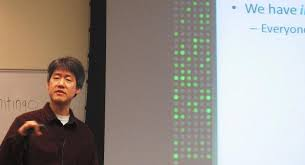
\includegraphics[width=.65\textwidth]{feedback-meetings-ms-research}
\caption{\emph{Crowd Feedback} \cite{Teevan:MobileFeedbackDuringPresentation} used during a presentation. The bar next to the slides shows one dot per participant in the meeting. The feedback dots fade out over time.}
\label{fig:related-work-crowd-feedback}
\end{figure}
% ADD MOBILE INTERFACE TOO AND MAKE PICTURE LOOK BETTARRR

\emph{Crowd Feedback} \cite{Teevan:MobileFeedbackDuringPresentation}, on the other side, is a system for displaying continuous, real-time feedback to the speaker in presentations. A responsive web application with a like and dislike button controls the feedback-system. The participants' reactions are shown with a red (dislike) or green (like) dot for each attendee in a sidebar next to the presentation slides (see figure \ref{fig:related-work-crowd-feedback}). An evaluation of the system showed that the participants felt more engaged with the presentation and connected to other listeners. Many users stated only having the possibility to like or dislike did not reflect enough options and that a button related to the speech pace might have helped. It was also noted that the sidebar was perceived as disturbing and made it harder to pay close attention to the presentation. This study and its conclusions have inspired the implementation of an instant feedback mechanism for listeners in the present work, however, instead of only having the binary like and dislike, the reactions are based on emojis, allowing for more insightful feedback.

The third study conducted by Microsoft Research concerns itself with the navigation through slides: \emph{Office Social} \cite{Chattopadhyay:OfficeSocialRemoteControl}, a PowerPoint plugin with companion smartphone app, allows presenters and listeners to navigate through PowerPoint slides using their mobile phones. Members of the audience can either browse the slides privately, or take over the control of the presented slides, allowing them to effictively steer the presentation or discussion. As in the present approach, Chattopadhyay et al.'s software allows members of the audience to review the slides privately, making it possible for latecomers to catch up and to generally estimate the length and direction of the talk. However, as their interface focuses on the navigation between slides, the preview of the slides is fairly small. Our approach tries to focus on the content of the slide and instead of offering big buttons to navigate around, makes use of intuitive swipe gestures. Another disadvantage is the overhead of having to download a smartphone application before the start of a presentation, as well as the limitation of the application only being available for Windows Phones.

\begin{figure}
\centering
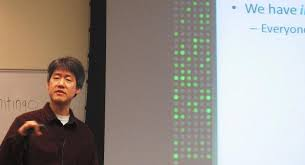
\includegraphics[width=.65\textwidth]{feedback-meetings-ms-research}
\caption{\emph{Office Social} \cite{Chattopadhyay:OfficeSocialRemoteControl}'s smartphone app interface. A preview of the slide is shown on top, followed by big buttons for navigating between slides.}
\label{fig:related-work-crowd-feedback}
\end{figure}

\section{General presentations}
Since lectures and meetings both are very specific forms of presentations, a few paragraphs should also be dedicated to general approaches in this third subsection.
One publication, which concentrates on polling and their real-time evaluation and rendering is \cite{Inoue:RealTimeQuestionnaire}: Inoue et al. present a system which distributes \emph{Microsoft PowerPoint} presentations using modern web-technologies while making it possible to alter and update the slides in presentation mode. This way questionnaires can be answered and their results displayed in real-time. Additionally, members of the audience can add annotations (both handwritten and digital) to slides. Although this approach seems very promising, pictures, videos and other types of media are ignored entirely. Moreover the interface seems too complicated to be displayed on small devices and is therefore only usable on laptops and maybe tablets.

Two more products, though not subject to scientfic research and more commercial than the approaches presented so far, are \emph{Mentimeter}\footnote{\url{http://www.mentimeter.com/}} and \emph{sli.do}\footnote{\url{http://sli.do}}. Both tools are web applications with real-time polling support, usable in any presentation. Both systems work very similarly: listeners go to the respective website and enter a presentation code to then be connected to the live voting. A handy feature Mentimeter offers is to query the device's location to determine the right presentation. Sli.do on the other hand also supports questions from the audience, which can be up-voted by the listeners, making it easy for speakers and participants in podium-discussions to answer the most relevant questions. Moreover, additionally to multiple-choice polls, sli.do also supports open questions and ratings. While the creators of Mentimeter provide a PowerPoint plugin, sli.do is not directly linked to any presentations. However, the popular canvas-based presentation-tool prezi\footnote{\url{http://prezi.com}}, offers seamless integration with the application. It is worth noting that prezi itself already offers mobile features out of the box: Presentations can be controlled remotely from the speaker's phone or tablet as well as be viewed and followed by members of the audience in real time, using a mobile application.

More web-based presentation tools include \emph{Google Slides}\footnote{\url{http://www.google.com/slides/about/}} and \emph{PowerPoint Online}\footnote{\url{http://office.live.com/start/PowerPoint.aspx}}. While PowerPoint Online seems to only offer a simplyfied version of the desktop application online, Google Slides also provides mobile features such as editing and authoring slides on phones or tablets and controlling them remotely.

To conclude this chapter, a few words should also be said about the JavaScript presentation library \emph{reveal.js}\footnote{\url{http://lab.hakim.se/reveal-js/}} and its accompanying visual edior \emph{slides}\footnote{\url{http://slides.com/}}. Reveal.js offers features such as remote controlling slides for the speaker and following presentations on personal devices for members of the audience. However, the installation to achieve the latter so-called \emph{multiplexing} functionality, is fairly complex and involves setting up a socket-io server, running the master-presentation statically and locally and uploading a client version of the presentation to a publicly accessible server. Reveal.js offers a decent online presentation library and could have served as a starting-point for the project presented in this thesis. However, due to their closed environment, tightly coupled code and lacking support for extensibility, we decided to instead implement an own presentation library (see chapter \ref{cha:implementation}, section \ref{sec:implementation-technologies-unveil}).
\chapter{Interactive Mechanisms}
\label{cha:mechanisms}

In a first step of identifying possible mechanisms which could make presentations more engaging and interactive, we analysed different types of presentations. There are several factors which determine these types, such as the size of the audience, the environment around and purpose of the presentation as well as the speaker and audience. In the following these factors will be described shortly to then present and discuss mechanisms these could profit from most.

\section{Factors}

\subsection{Audience Size}
One aspect which plays an important role in the type of presentation and thereby the interactive mechanisms applicable is the size of the audience. Different challenges present themselves, depending on the amount of listeners: While there might be a debate between speaker and audience in small group sizes, it is hard for audience members to directly communicate with a speaker during conferences or in large lecture halls. Shy or introvert attendees might remain unheard \cite{Bry:Backstage} and only a usually randomly chosen subset of people get the opportunity to ask audience questions after talks in conferences. At the same time estimating the audience's knowledge and interest as well as the general mood gets increasingly difficult both for the presenter and attendee as the number of participants rises. Additionally to the interaction between speaker and audience, another important factor is listener-listener interaction \cite{Moore:ThreeTypesOfInteraction}. Group-dynamics largly depend on the audience size and smaller groups usually perform better than big ones \cite{Phillips:GroupProblemSolving}.
The general conclusion therefore is that big audiences struggle to connect and interact with the speaker and each other and interactive tools must aim to strengthen the bidirectional bond between presenter and listeners. In smaller groups, on the other hand, the focus should be put on supporting the already existing dialogue and exchange between all participants of the presentation. As peer-pressure might rise in smaller groups and the better listeners know each other, ways of anonymously contributing to the outcome or flow of a presentation become more important.

\subsection{Presentation Environment}
% Remote vs co-located!
% setting: classroom vs. meeting vs. conference etc.
The environment of a presentation is described by all factors surrounding the presentation. One of them is the setting a talk is given in, in other words, if it is embedded in a meeting, a talk at a conference or a lecture at school or university. Other aspects worth considering are whether the audience is co-located or distributed and which technologies are available. As this work concerns itself only with mobile devices in the context of co-located presentations, difficulties added through remote presentations as well as missing technical equipment will be disregarded in this section. Instead, a closer look will be taken at the setting: In a lecture, it is desirable to measure the students' participation and engagement, as well as their understanding of a topic. In meetings, on the other hand, interactive mechanisms are more likely to aim for the promotion of collaboration between all participants. Conferences might search to foster the interactivity between attendees, to support networking. Instead of taking all possible scenarios into consideration, this work concentrates on business-related settings and explores mechanisms which foster collaboration.

Another part is the purpose of a presentation: McClain \cite{McClain:TypeOfPresentations} identifies four major types: informational, motivational, pursuasive and sales. According to him, informational presentations search to educate the listeners, while motivational speeches try to inspire the audience to take action. Pursuasive talks usually present new ideas or directions and have the goal of making the listeners re-think old approaches and consider or even embrace new ones. Sales presentations, lastly, often use elements of the other three categories with the aim of ``obtaining a decision at the presentation's end'' \cite{McClain:TypeOfPresentations}. While motivational, pursuasive and to some extend sales presentations often operate on an emotional level in the present moment, informational talks often include a way for listeners to re-visit the taught material through transcripts, lecture notes or handouts. Moreover, motivational, pursuasive and sales presentations focus on the goal of getting the audience to take action and therefore put more emphasise on the listeners than content-centric informational speeches. This creates two very distinctive needs for interactive mechanisms: on one side the ability for the audience to actively shape the path of the presentation, on the other hand the possibility to re-visit presentation slides (potentially including notes and additional material), after the end of a talk.

% welches material wird mitgenommen? wie können lectures erinnert werden? welches material nehmen wir mit? --> nachbereitung/handouts!
% motivational und pursuasive: mehr im hier und jetzt, memorable auf gefühlsebene!
% in manchen ist es einfacher das Publikum leiten zu lassen als in anderen (motivational & pursuasive)

\subsection{Speaker and Audience}
% tech savvyness for audience
% spontanität and flexibility for speaker --> when do I take questions? überfordert? etc.
% level of formality!
The last factor taken into consideration in this chapter are the speaker and listeners themselves. Depending on the individual interest, but also character traits such as introversion, listeners will be more or less likely to engage in a presentation actively \cite{Bry:Backstage}. The inter-attendee relationship as well as the relationship between attendees and speaker also plays a role in which mechanisms are appreciated and which are not \cite{Moore:ThreeTypesOfInteraction}: while it is common for listeners to jump into the role of the presenter in meetings with flat-hierarchies, the same behaviour is a rare sight in lectures or might even be deemed inappropriate or rude in more formal settings. When taking the speaker into consideration, the set of tools needed are more sophisticated than the ones necessary to only follow a presentation: Foremostly, speakers need a way of navigating through slide decks. It is desirable to have an overview of the entire presentation and while listeners only concentrate on the current slide, many speakers rely on notes or use timers, which also need to be placed in the interface.
Moreover, the presenter's personal traits, experience and bluntly talent, play a central role in the successful deployment of interactive mechanisms: the flexibility, confidence and technological expertise of a presenter all determine how distracting or even stressful certain features are perceived as and whether a speaker is able to react to these spontaniously \cite{Wacker:PresenterExperience}. It is therefore crucial to give speakers the ability to turn said mechanisms on and off. An important challenge which also arises with this question is how to design these mechanisms in a way that is neither perceived as intrusive nor interrupting (this will be discussed in more detail in chapter \ref{cha:design}).
To summarise, when developing interaction tools, it is vital to take a participant's personality and their relationship to other ones into consideration. In the context of presentations, shy listeners should be given tools to make them heard; presenters need full control of the mechanisms provided.

\section{Resulting Mechanisms}
With these aspects and challenges in mind, a multitude of different mechanisms can be derived. Although many more are thinkable, this section concentrates on the ones implemented in course of the thesis project. However, we will try to point out other possible features and provide resources to projects focusing on these. One point to keep in mind is that not all of the presented mechanisms work equally well in every environment but instead have scenarios they are best suited for and others in which they are practically rendered redundant. The ideal settings and key advantages of each of these mechanisms are summarised in table \ref{tab:mechanisms}.

% Speaker: Remote control
% Speaker: See next slide right and down, notes on phone or tablet/laptop!
%
% Following slides on personal device
% Questions
% Anonymity
% Polls
% Reactions (Emojis) -- tell how these can engage the people more, not only about how they provide feedback to presenter!
% Annotating slides and sharing content (!) --> not really studied yet, so cool!

\subsection{Remote Control}
One mechanism of special importance for speakers is the ability to control slides and navigate through them. As many presentations involve more than just one speaker and can profit from sharing control over slides with others \cite{Chattopadhyay:OfficeSocialRemoteControl}, any amount of presenters should be able to be connected at any given point. Controlling should be possible from any personal device, may it be a laptop, tablet or mobile phone, giving the speakers maximal freedom.

While using arrow-keys in a desktop environment feels natural to navigate between slides, the native equivalent on touch-devices are swipe gestures. These are more accurately and faster when operating a phone with one hand \cite{Lai:SingleHandedThumbInteraction} and are less prone to error when used eye-free \cite{Negulescu:TapSwipeMove} and should therefore be prefered over buttons, clustering the interface.

\subsection{Following Slides}
% also gives latecomers the chance...
For members of the audience, one important feature, both in the context of re-visiting slides, to accommodate individual learning paces \cite{Cheng:TreebasedOnlinePresentations} and even to give latecomers a chance to catch up with the presentation \cite{Chattopadhyay:OfficeSocialRemoteControl}, is to be able to independently follow the slides. This should again be possible on any personal device and focus on the slide content, in a way that maintains the readibility of all text. The mechanism can be designed in many different ways and could even allow listeners to remote control the presentation \cite{Chattopadhyay:OfficeSocialRemoteControl}, our implementation however only provides individual slide navigation on the personal device. Additionally, the progress of the presentation should always be synchronised with the individual devices, allowing listeners to truely follow along. This basic mechanism can be extended to offer features such as turning the synchronisation on and off (effectively allowing to navigate freely and jump back to the presenter's state) or to only allow listeners to see the last slide the presenter has already shown.

\subsection{Paths}
Also connected to navigation and following slides is the possibility to offer different paths through the presentation. Especially in informational talks these can account for different backgrounds and levels of knowledge in the audience, they however, also make it possible to get listeners more involved in shaping the presentation. Paths should both be accessible to each audience member individually (for further reference or to catch up on a topic), as well as on the projector (e.g. by polling, as discussed in the next subsection).
The possibility to flexibly navigate through a presentation has proven to be one of the biggest advantages of canvas-based presentations \cite{Lichtschlag:CanvasPresentationsInTheWild} and have a wide field of application. The scenarios this thesis concentrates on are the following: On one hand, the paths can cover different levels of details (e.g. \emph{overview}, \emph{regular} and \emph{detailed}), as well as providing a way of skipping certain slides without having to navigate through all of them (e.g. skipping the introduction). Another option would be to let the audience decide between entirely different topics, depending on their personal interest. While canvas-based presentation tools like Prezi innately offer this flexibilty, slide-based tools often only make this behaviour possible by manually skipping over slides, which can interrupt the flow of the presentation \cite{Dieberger:NarrativeFlow}. PowerPoint extensions enabeling advanced forms of navigation, as well as the presenter looking through slides before projecting them are discussed in \cite{Dieberger:NarrativeFlow}, \cite{Nelson:PalettePaperInterface} and \cite{Signer:PaperPoint}, the latter, however, will not be part of our implementation.

\subsection{Audience Questions}
Another feature, well-suited for informative talks, is the possibility for members of the audience to ask questions. Another scenarios are big crowds, in which it is hard to be heard as an individual. A tool specifically designed for such settings is sli.do, which was already introduced in chapter \ref{cha:related-work} section \ref{sec:related-work-general}.
More generally, such mechanism should enable members of the audience to submit questions for the presenter to answer. These questions should either be displayed directly, or collected for the presenter to go through at the end of the presentation, depending on their preference and flexibility. This mechanism also highly depends on the presentation environment: In a classroom, questions should be answered immediately, while conferences usually only allow them at the end of talks. Questions could moreover only be visible to the presenter, or every participant. Concentrating on business-related settings, we propose a question feature which allows audience members to submit questions at any point of the presentation. These should be accessible for every attendee, to spark others' interest and participation. From the presenter's point of view, questions should be displayable instantly, at the end of the talk or any time inbetween, leaving the decision when to react to questions to each individual speaker.

% what does it mean for the presenter - take questions right away or in the end?

\subsection{Polls}
Another possibility to ask questions is polling. Although polls might also be generated by listeners, we propose a mechanism which lets the speaker create them. To give presenters more flexibility and because questions often only arise during talks \cite{Esponda:ElectronicVotingOnTheFly}, these surveys should be creatable in the preparation for a speech as well as on-the-fly, during presentations. This mechanism can help getting to know ones listeners (relationship between listeners and speaker), as well as estimate a crowd's mood (big audiences) and is especially useful in combination with paths. If supporting anonymous voting, relying on electronical aids instead of raising hands can also be benificial in smaller groups \cite{Esponda:ElectronicVotingOnTheFly}.
While a big number of different polling mechanisms are conceivable (open questions, ratings, multiple choice, as well as different ways of visualising the results), single choice voting and visualisation in a bar-chart serve as a starting point for our approach. Another detail lies in when the results are presented: they can either be rendered as soon as a user chooses his or her answer or only after everybody has given their votes.
To summarise, the identified requirements for such mechanism are creation beforehands and during the presentation, real-time polling and data-visualisation as well as anonymity of the voting process.

\subsection{Reactions}
As described before, especially bigger crowds suffer from a lack of interaction possibilities between speaker and audience but also between members of the audience. While the latter is discussed in \cite{Bry:Backstage}, the present work focuses on the interaction between speaker and listeners. Besides the difficulity of asking questions, which was already covered, the main problem for the presenter is to estimate the crowd's mood, which is why we suggest a mechanism that lets attendees send real-time feedback to the speaker. This functionality is based on \cite{Teevan:MobileFeedbackDuringPresentation}; as highlighted by Teevan et al., however, their simplistic approach of just offering \emph{likes} and \emph{dislikes} is not faceted enough to represet the full range of emotions listeners can feel during a presentation. It is therefore important to provide more detailed feedback.
These reactions can either be displayed only to the speaker, or to the entire audience. The latter might distract listeners \cite{Teevan:MobileFeedbackDuringPresentation}, however, also holds the potential to encourage others to also react to the current slide and strenghten listener-listener bonding. While this mechanism is expected to work well in bigger crowds, it will likely introduce an unnecessary technical burden to smaller groups, in which it is easier to estimate the attendees' mood. 

\subsection{Content Sharing}
In contrast to live reactions and questions, content sharing is especially suited for smaller audiences. As discussed before, tools for smaller groups should strengthen the already possible dialogue between all participants. These scenarios make it possible for listeners to actively get involved in the presentation and not only shape the path through, but also the content of such. While adding subslides to a slide deck after a presentation \cite{Cheng:TreebasedOnlinePresentations} and text-based annotations \cite{Inoue:RealTimeQuestionnaire, Myers:CollaborationPDAs} during talks have already been discussed in previous work, to our knowledge, no other study has concerned itself with the possibility of adding listener-generated slides and multi-media content in live presentations. While being an exciting opportunity to explore a widely untouched research subject, this mechanism empowers listeners and transforms presentations entirely by combining classic slides with brainstroming-like interactions and related multi-media content. While the potential of this mechanism will be further discussed in chapter \ref{cha:conclusion}, the requirements for this functionality should shortly be defined: It should be possible for any listener to add their own content to any slide. This content includes text, websites (per link), videos and uploaded images (e.g. taken with their personal devices). Presenters should have a way of deciding whether to accept the contribution and if it should be added as a subslide or main slide. Moreover, this mechanism requires a lot of flexibility from the speaker, which is why it is important to allow them to turn off or silence the functionality, providing sensible fallbacks. While content sharing can transform a presentation into an interactive and collaborative effort in smaller groups, the functionality will likely lead to chaos in big groups, without further interface changes.

Now that the implemented mechanisms are clarified and their requirements defined, the next chapter deals with the design and user experience of the application.

\begin{table}
\caption{Overview of resulting mechanisms, with their key advantages and optimal usage scenarios.}
\label{tab:mechanisms}
\centering
\def\rr{\rightskip=0pt plus1em \spaceskip=.3333em \xspaceskip=.5em\relax}
\setlength{\tabcolsep}{1ex}
\def\arraystretch{1.20}
\setlength{\tabcolsep}{1ex}
\small
\begin{english}
\begin{tabular}{|p{0.2\textwidth}|p{0.35\textwidth}|p{0.35\textwidth}|}
\hline
   \multicolumn{1}{|c}{\emph{Mechanism}} &
   \multicolumn{1}{|c}{\emph{Improvements}} &
   \multicolumn{1}{|c|}{\emph{Ideal Scenario}} \\
\hline\hline
   {\rr Remote Control} &
   {\rr More flexibility for presenter(s)} &
   {\rr Any, especially mutli-speaker presentations}
   \\
\hline
   {\rr Following Slides} &
   {\rr Accounts for individual pace; can replace hand-outs} &
   {\rr Any, especially informational presentations for later revision}
  \\
\hline
   {\rr Paths} &
   {\rr Interactivity and possibility to shape presentation for audience} &
   {\rr Any, especially informational}
   \\
\hline
   {\rr Audience Questions} &
   {\rr Anonymity; possibility to be heard in big crowds } &
   {\rr Big audiences; small groups for anonymity}
  \\
\hline
   {\rr Polls} &
   {\rr Bond between speaker and audience by querying listeners' interest, mood and knowledge} &
   {\rr Usage with paths; big audiences; small groups for anonymity}
   \\
\hline
   {\rr Reactions} &
   {\rr Speaker-audience and listener-listener interaction} &
   {\rr Big audiences}
   \\
\hline
   {\rr Content Sharing} &
   {\rr Possibility to shape presentation for audience; slide-content by adding related resources} &
   {\rr Small groups}
   \\
\hline
\end{tabular}
\end{english}
\end{table}
\chapter{Application Design}
\label{cha:design}

After defining the mechanisms which will be implemented, in a next step, the general application flow will be described, as well as offering insight into the user experience design of the parts of the application.

\section{Application Flow}
The flow and usage of the application is separated into two parts: the creation and authoring of the presentation and giving the presentation. Because the technical details of how slide decks are composed are covered in chapter \ref{cha:implementation}, this chapter focuses on the user interface and interaction design of the software from the speaker's and the audience's point of view, during the presentation.

The slides are generally served either from a publicly accessible server or, if all participants are in the same network, locally from the presenter's computer. This means, at the beginning of the presentation, all attendees have to navigate their personal devices' browsers to the set up address (usually a combination of IP address and port). To make this step easier, QR codes pointing to the address can be shown on the first slide or e-mails can be sent out to all participants before the start of the presentation.

The software supports three different modes out of the box: default (i.e. listener), presenter and projector mode. Depending on the mode, a certain set of features are activated, allowing the presenter to have a different interface and more controls than the listeners and to only show the current slide in projector mode. Modes are activated via query-strings in the url: The speaker navigates the browser of the device connected to the projector to the url of the presentation and adds the query parameter \printtt{mode=projector}. On his or her personal device, the mode is set to \printtt{presenter}. If no query parameter is given, the application defaults to the listener mode.

% Base CSS: responsive, if content is too big, everything is uniformly scaled.


% Application Flow, Modes, How does the application work in general?
% Design aspects, sketches, wireframes, thoughts and überlegungen behind design details

% As described before, it is important for the presenter to be in full control of all mechanisms --> make it easy to add or remove them and to configure!

% Wacker: research has shown that technological problems are the main reason for negative presentation experiences for the speaker. ``Therefore, presentation software should take special care to avoid technological problems and assist the presenter if they should occur''

% We believe it is still important for the speaker to have an overview of the current slide as well as upcoming ones and be able to see notes on the presenter interface

% General requirements: be viewable on every device, work in real-time!

% Emojis
% Find more studies about this! think: facebook, the conference Paulo went to etc. (maybe add photo of audience showing emoji faces!)
% It is therefore important to provide more detailed feedback. Following the evaluation in \cite{Teevan:MobileFeedbackDuringPresentation}, the mechanism proposed in this thesis offers three emotions (approval, laughter, boredom) and three request types (louder, speed up, slow down).

% Polls: Describe why freeze navigation while voting and only allow voting when started by presenter
\chapter{Implementation}
\label{cha:implementation}
% short overview; why web -- use references!
% speak about quick prototyping possibilities and how it's easier to roll out updates and how nobody needs to download an app on their phone to interact with the presentation
% say something about open source and why all the code is online on github!

This chapter dives into the technical implementation details of the thesis project and gives an overview of the used technologies and explains why these were chosen over others. Like many other projects in this area \cite{Bry:Backstage, Cheng:TreebasedOnlinePresentations, Esponda:ElectronicVotingOnTheFly, Inoue:RealTimeQuestionnaire, Teevan:MobileFeedbackDuringPresentation, Triglianos:InteractiveWebPresentationsImpress}, the project is realised as a web application. This has many advantages, from modern web technologies' quick prototyping capabilities to the web's general cross-platform and cross-device nature, the project has profitted from the dynamicity of the internet and the rapid evolvement of JavaScript over the past years.
Although native sharing features of smartphones cannot be used due to the choice of platform, the advantages that come with this decision outweigh the disadvantages, as I like to think for both users and developers: as nobody has to download any apps to their devices, it is easier to bring the audience to use the developed application \cite{Triglianos:InteractiveWebPresentationsImpress}. The major advantages for developers on one hand is the ability to only concentrate on one platform, instead of developing different applications for different operating systems (mobile and desktop), on the other hand the web is built for rapid prototyping as it is extremely easy and fast to roll out new updates, without distributing them through the App Store or Play Store and without the need for users to manually update their apps. The chosen JavaScript library React, however, offers the possibility to cross-compile applications to different devices using React Native, which should make it fairly easy to port the existing web application in the future.

As it was important to achieve fast response times and because \emph{WebSockets} have successfully been deployed in the real-time features of other presentation tools \cite{Inoue:RealTimeQuestionnaire, Triglianos:InteractiveWebPresentationsImpress}, this technology has also been used in this thesis project, to handle the communication between clients and server.

A few words should also be said about the distribution of this project. Without the vibrant open-source community, many of the frameworks and libraries used in this project would not exist. For this reason and to give back to this community, all the libraries developed during this project are published as open-source on my GitHub profile\footnote{\href{https://github.com/irisSchaffer?tab=repositories}{\textsf{https://github.com/irisSchaffer/}}} and freely available for anyone to use.

\section{Project Scope}
\label{sec:implementation-scope}
% What's the general scope of the project? Why is everything on the client and 
% not the server? etc.
Before jumping into technical details, the scope of the project should be discussed. As the aim of the present work is to explore ways of incorporating mobile devices into presentation workflows, the goal of the project was to use an easily extensible presentation library to then build the mechanisms discussed in the previous chapter.
As the focus was placed on the interaction possibilities between speaker and audience, the creation of the presentation for the speaker or the management of slides and presentations were out of scope. Therefore the server used for connecting different users to the presentation was kept as simple as possible, allowing any potential other developer to work with their own servers and technology stacks.

In total, a system with several ways of interacting with the presentation from mobile or desktop devices was created, putting emphasise on mobile-optimised views and navigation possibilities. This system includes synchronisation of navigation state and state changes between viewers and speaker, the possibility to add sub-slides during the presentation for the audience, a speaker-view showing the next slides and controls, real-time voting (both created on-the-fly and prepared beforehands) and the possibility to create different paths through the presentation. In the following the technologies used in the project will be analysed and described to then discuss implementation details, problems and solutions of the mentioned components.

\section{Technologies}
\label{sec:implementation-technologies}
% Which technologies were chosen and why?
% How do they generally work? To a level on which the reader can
% understand the rest of the implementation details
% A few words about responsive design and media queries would probs be good
% a few words about babel and es6

The project generally tries to follow best-practices in web development and utilises modern CSS3 and JavaScript features and frameworks. The software is written in ECMA\-Script\-2015, makes use of the \emph{node package manager}\footnote{\url{https://www.npmjs.com/}}(short \emph{npm}) for managing dependencies and \emph{Babel} to transpile to ECMA\-Script\-5. Additonally to relying on CSS3 features, this project also uses \emph{Sass}\footnote{\url{http://sass-lang.com/}} as a CSS pre-processor. Media-queries allow for mobile-friendly views.

On the front end, which this project focuses on, the JavaScript library \emph{React} is the framework of choice, additionally applying the \emph{reactive programming} paradigm using \emph{RxJS} to allow for a simpler interface for event-driven operations. The communication between client and server is handled by \emph{socket.io}\footnote{\url{http://socket.io/}}.
This section tries to introduce the reader to the main technologies used to establish a base on which the following technical implementation details can be understood.

\subsection[ECMAScript2015 and Babel]%
             {ECMAScript2015 and Babel%
             \protect\footnote{\url{https://babeljs.io/}}}%
\label{sec:implementation-technologies-es6}
% it's a recommendation, but it takes long until browsers implement it and users update their browsers.
JavaScript undoubtly is an integral part of front end web development and since the emergence of server-side JavaScript with Node.js\footnote{\url{https://nodejs.org/en/}} and its package manager npm has developed into a programming language widely used by web developers \cite{gpm-meta-transcompiler}. Both PYPL\footnote{\url{http://pypl.github.io/PYPL.html}} and TIOBE\footnote{\url{http://www.tiobe.com/tiobe_index}} programming language indices rank JavaScript among the top 10 programming languages (PYPL at 5, TIOBE at 7 at the time of writing) \cite{gpm-meta-transcompiler}. Stack Overflow's 2015 Developer Survey even places JavaScript as the number 1, most-used programming language with 54.4\% and JavaScript, Node.js and AngularJS\footnote{\url{https://angularjs.org/}} all three rank amongst the top 5 languages developers expressed an interest in developing with \cite{stackoverflow-developer-survey}.

However, like any front end technology, JavaScript suffers from slow end user adoption, as a multitude of browser versions exist for different devices and operating systems and many people still do not auto-update their browsers. Another factor is the time it takes for browser-vendors to implement new ECMAScript standards (the standard behind JavaScript) and roll out said updates. This is exactly what is happening with the new ECMAScript standard, ECMA-262, commonly known as ECMAScript 2015 or ES6: Although the General Assembly has adopted the new standard in June 2015 \cite{ecma2015}, \emph{Kangax' ECMAScript compatibility tables}\footnote{\url{https://kangax.github.io/compat-table/es6/}} still show a fairly low level of adoption, especially among mobile browsers. ES6 makes JavaScript easier and more efficient to write by providing new semantics for default values, arrow-functions, template-literals, the spread operator or object destructuring \cite{es6}. It also makes JavaScript easier to understand and safer to develop, with the introduction of block-scoped variables (\texttt{let} and \texttt{const}) and finally offers native support of modules and promises \cite{es6}.
As these features are all included in the new ECMAScript standard, it is safe to assume browser-vendors will implement them in the near future. Until then, developers who want to already make use of them, can \emph{transpile} ECMAScript 2015 code into ECMAScript 5, which is exactly what Babel does. With over $650000$ downloads in March 2015 (according to npm) and companies like Facebook, Netflix, Mozilla, Yahoo or PayPal using this transpiler \cite{babel-users}, Babel is the de facto standard solution to transpile to ECMAScript 5 and was also chosen for this project.

\subsection{Reactive Programming}
\label{sec:implementation-technologies-rxjs}

Another problem with JavaScript, although integral part of the reason for its high popularity, is its asynchronous nature. Especially when working with highly interactive parts, the prime example being user interfaces, sequential programming quickly gets too inflexible to handle complex, event-driven applications \cite{reactive-programming-survey}. But also on the server, the possibility to concurrently serve a multitude of different clients, is crucial. In these cases JavaScript offers \emph{event listeners} -- functions called once a certain event happens. However, these event listeners or \emph{asynchronous callback} \cite{reactive-programming-survey}, oftentimes executes more asynchronous code and in turn has to wait for another event, and another one, and another one... which can result in something known and dreaded by most any JavaScript developer: \emph{Callback Hell} (see programm \ref{prog:implementation-technologies-rxjs-callback-hell}).

\begin{program}
\caption{\emph{Callback Hell} -- Nested callbacks in JavaScript. Simplified method taken from a previous project, which authenticates a user, creates a new google calendar for them and then saves the user to one\'s own database, to then redirect them. \texttt{\{...\}} is used to shorten the code, error-handling was also omitted in the example for simplicity.}
\label{prog:implementation-technologies-rxjs-callback-hell}
\begin{JsCode}
router.get('/callback', function(req, res, next) {
  var code = req.query.code;
  var name = JSON.parse(req.query.state);

  // get token from oauth library
  oauth2Client.getToken(code, function (err, tokens) {
    // load configuration
    Configuration.findOne({}, function (err, configuration) {
      var calendar = google.calendar('v3');
      // save to google calendar
      calendar.calendars.insert({...}, function (err, cal) {
        var member = new Member({...});
        // save member to own database
        member.save(function(err, member) {
          return res.redirect(getRedirectionUrl(name) + '&success=true')
        });
      });
    });
  });
});
\end{JsCode}
\end{program}

Different approaches have been employed to lower the hurdle of writing asynchronous code, one of them being \emph{promises}: A promise is a value, yet to be computed \cite{reactive-vs-promises}. A promise can be a) pending (if it has not been assigned a value yet), b) resolved (if it has been assigned a value) or c) rejected (if an error occurred). In ECMAScript 2015 promises these objects can then be queued using the \texttt{then} keyword, to execute asynchronous code in a certain sequence (see programm \ref{prog:implementation-technologies-rxjs-promises}).

\begin{program}
\caption{\emph{Promises} -- Simple example of chaining ECMAScript 2015 promises with \texttt{then} and \texttt{catch}.}
\label{prog:implementation-technologies-rxjs-promises}
\begin{JsCode}
var promise = new Promise(function(resolve, reject) {
  asyncCall(function(error, data) {
    if (error) {
      reject(error); // reject the pending promise
    } else {
      resolve(data); // resolve the pending promise
    }
  })
})

promise
  .then(function(data) {
    // this is executed after asyncCall returns
    // other asyncronous calls can be placed here
  })
  .catch(function(error) {
    // this is executed if an error occurs somwehere along the way
  })
\end{JsCode}
\end{program}

However, promises can still create nested callbacks, especially when chaining promises that rely on other promises' resolution \cite{reactive-vs-promises}. This is where \emph{reactive programming} comes in: The reactive programming paradigm works with streams of events, in which every event is handled as a new value and all other parts depending on this value are re-computed upon arrival of such a new value. To demonstrate this I would like to use Bainomugisha et al.'s illustrative example of a simple addition \cite{reactive-programming-survey}:

\begin{JsCode}
var v1 = 1
var v2 = 2
var v3 = var1 + var 2
\end{JsCode}
%
In sequentially executed code, \texttt{v3} will hold the value $3$, no matter if or how \texttt{v1} or \texttt{v2} change. In reactive programming, however, \texttt{v3} will be re-computed as soon as either one of the values it depends on change \cite{reactive-programming-survey}. This way for a drag-and-drop feature, for example, the move of the mouse, continuously sending its location, could directly alter the position of an element in a page. JavaScript does not directly support reactive programming, but other, more functional languages, which can be transpiled to JavaScript, do. Another way of adding reactive programming concepts to JavaScript is using a library, such as \emph{Bacon.js}\footnote{\url{https://baconjs.github.io/}} or the one chosen for this project, \emph{ReactiveX}\footnote{\url{http://reactivex.io/}}. ReactiveX provides libraries for a multitude of different programming languages, C#, C++, Java and of course JavaScript among them. The latter, called \emph{The Reactive Extensions for JavaScript} or short \emph{RxJs}, allows for the simple creation of event streams (\emph{Observables}) from browser events or promises directly and uses the same method names JavaScript developers are familiar with from array-methods, most notably and well-known \texttt{map}, to apply a method to every element in the incoming stream and \texttt{filter}, to only let a subset of events pass. These methods can be chained to sequentially alter a value (see programm \ref{prog:implementation-technologies-rxjs}).

\begin{program}
\caption{\emph{RxJS} -- simplified example of the touch controls used to swipe to the next or previous slide. An Observable is created from the browser's \texttt{touchmove} event and is then transformed with \texttt{map} and \texttt{filter}, to in the end call the \texttt{navigate()} method with the direction the user swiped into.}
\label{prog:implementation-technologies-rxjs}
\begin{JsCode}
this.moveObservable = Observable.fromEvent(document, 'touchmove')
  // data: event object with array of touches
  .filter(this.touchStarted) // only procede if touchstart is set to true
  .map(this.toXY) // transform initial event data to latest touch's xy position
  // data: \{x: xPosition, y: yPosition\}
  .map(this.toDirection) // transform xy position to direction literal
  // data: right/left/up/down
  .do(this.resetTouchStart) // set this.touchStarted to false
  // data: right/left/up/down
  .subscribe(this.navigate); // call this.navigate() with direction data
\end{JsCode}
\end{program}

Additionally to Observables, RxJs also knows \emph{Subjects}, which combine both a source of events and a consumer of such. Subjects are Observables, but also Observers at the same time and can be used to broadcast values to several consumers \cite{rxjs-docu}.

\subsection[React]%
             {React%
             \protect\footnote{\url{https://facebook.github.io/react/index.html}}}%
\label{sec:implementation-technologies-react}
% explain base concept of having re-usable components and how they are defined!
% get some HTML code in there :)

As this project concentrates on the front end, a mature JavaScript framework was searched for. After previous experience with the big and complex, but slow AngularJS, because of promising performance benchmarks \cite{react-benchmarks} and simply to explore new JavaScript libraries, I decided to give React a try. Since Facebook started developing React in 2013, it has challenged existing approaches and set new standards in front end web development \cite{introduction-to-react}. Instead of creating an entire MVC framework for the front end, React really concentrates on the view by offering a way of creating independent, lightweight view components. This gives React the huge advantage of beating other front end frameworks by far in performance benchmarks \cite{react-benchmarks}. Moreover, \emph{React Native}\footnote{\url{https://facebook.github.io/react-native/}} would make it possible to port the application to different mobile operation systems fairly easily.
The arguably most important method these re-usable, lightweight components implement is the \texttt{render} method, defining what HTML or JSX\footnote{\url{https://facebook.github.io/jsx/}} should be rendered by the browser:
\begin{JsCode}
export default class HelloWorld extends Component {
  render() {
    return (<h1>Hello World!</h1>);
  }
}
\end{JsCode}
%
The created Component can then be rendered into the virtual React DOM, JSX makes it possible to simply use the name of the component to create it:
%
\begin{JsCode}
ReactDOM.render(
  <HelloWorld />,
  document.getElementsByTagName('body')[0]
);
\end{JsCode}
%
This would simply put an \texttt{h1} element with the text \texttt{Hello World!} into the \texttt{body} element of the HTML page. Additionally to the \texttt{render} method, components also have a \emph{state} and \emph{properties}(\texttt{props}), through which they can communicate with other components and maintain their inner state. \texttt{props} are passed in to the component during creation, in JSX this can be achieved by simply passing them in as XML attributes:
%
\begin{JsCode}
  <HelloWorld greeting="Hi" />
\end{JsCode}
%
This could in turn be used in the \texttt{HelloWorld} component's \texttt{render} method:
%
\begin{JsCode}
  render() {
    return (<h1>{this.props.greeting} World!</h1>);
  }
\end{JsCode}
%
The children of a component are also available through \texttt[this.props.children]. The \texttt{state} variable, on the other hand, is responsible for handling internal updates e.g. through user interaction \cite{react-docu}. To alter the state, the method \texttt{setState} can be used, which will cause an update and re-rendering of the component. So if in the above example, the word ``World'' should be changed to something else by the user, a text field with an event handler can be added inside the component:
%
\begin{JsCode}
// set default state and props...

componentWillMount() {
  // create observable from change event on input
  this.observable = Observable.fromEvent('change', this.refs.input)
    .pluck('target', 'value') // extract input text
    .subscribe(this.update) // call update with value
}

componentWillUnmount() { this.observable.unsubscribe() }

update(text) { this.setState({name: text}) }

render = () => (
  <div>
    <h1>{this.props.greeting} {this.state.name}!</h1>
    <input value={this.state.name} ref="input" />
  </div>
)
\end{JsCode}
%
Now, whenever a user changes the text in the \texttt{input} field, the RxJS Observable will receive a new value (a change event). The \texttt{value} of the field is extracted on line $6$ and used to then update the state in the \texttt{update} method, which is implicitly called with the value passed through the Observable chain.

The two methods \texttt{com\-po\-nent\-Will\-Mount}, \texttt{com\-po\-nent\-Will\-Un\-mount} as well as \texttt{com\-po\-nent\-Did\-Mount}, \texttt{should\-Com\-po\-nent\-Up\-date}, \texttt{com\-po\-nent\-Will\-Up\-date}, \texttt{com\-po\-nent\-Did\-Up\-date} and \texttt{com\-po\-nent\-Will\-Re\-ceive\-Props} are \emph{lifecycle methods}, called whenever the component is created, updated or destroyed.

As an end note on React, and a transition to the core presentation library, I want to add that React components can be nested, which is at the core of the project developed for the present thesis. To make it as easy as possible for other developers to use the created libraries, a presentation is built just as a usual HTML page, using JSX to reference the custom React components (see program \ref{prog:implementation-technologies-react}).
%
\begin{program}
\caption{Nested React components. In this example, a 1-slide-long presentation is created.}
\label{prog:implementation-technologies-react}
\begin{JsCode}
<UnveilApp>
  <Slide name="start">
    <h1>Unveil</h1>
    <h2>a meta presentation</h2>
    <Notes>Greet people and welcome everyone</Notes>
  </Slide>
</UnveilApp>
\end{JsCode}
\end{program}

\subsection[unveil.js]%
             {unveil.js%
             \protect\footnote{\url{https://github.com/ostera/unveil.js}}}    
\label{sec:implementation-technologies-unveil}
% explain how this was developed together with Leandro, explain general parts like router, navigator, UnveilApp
% Give overview over controls in here.
% Also talk about the mobile style sheets / responsive design and the TouchControls, which I also implemented alone.
% (mention that this part is unit tested with jest(https://facebook.github.io/jest/))

As a presentation layer, this project uses the open-source JavaScript library \textit{unveil.js}, which was developed by Leandro Ostera and myself in the beginning of the project and which I extended and adapted to my needs in an own fork\footnote{\url{https://github.com/irisSchaffer/unveil.js}} during the project. This fork will be covered in section \ref{sec:implementation-unveil} of this chapter, until then, a short overview of the different parts of unveil.js is given and key concepts of the library are discussed. Screenshots of what unveil.js looks like can be found in figure \ref{fig:implementation-technologies-unveil-screenshots}.

%\begin{figure}
%\centering\small
%\begin{tabular}{cc}
%\FramePic{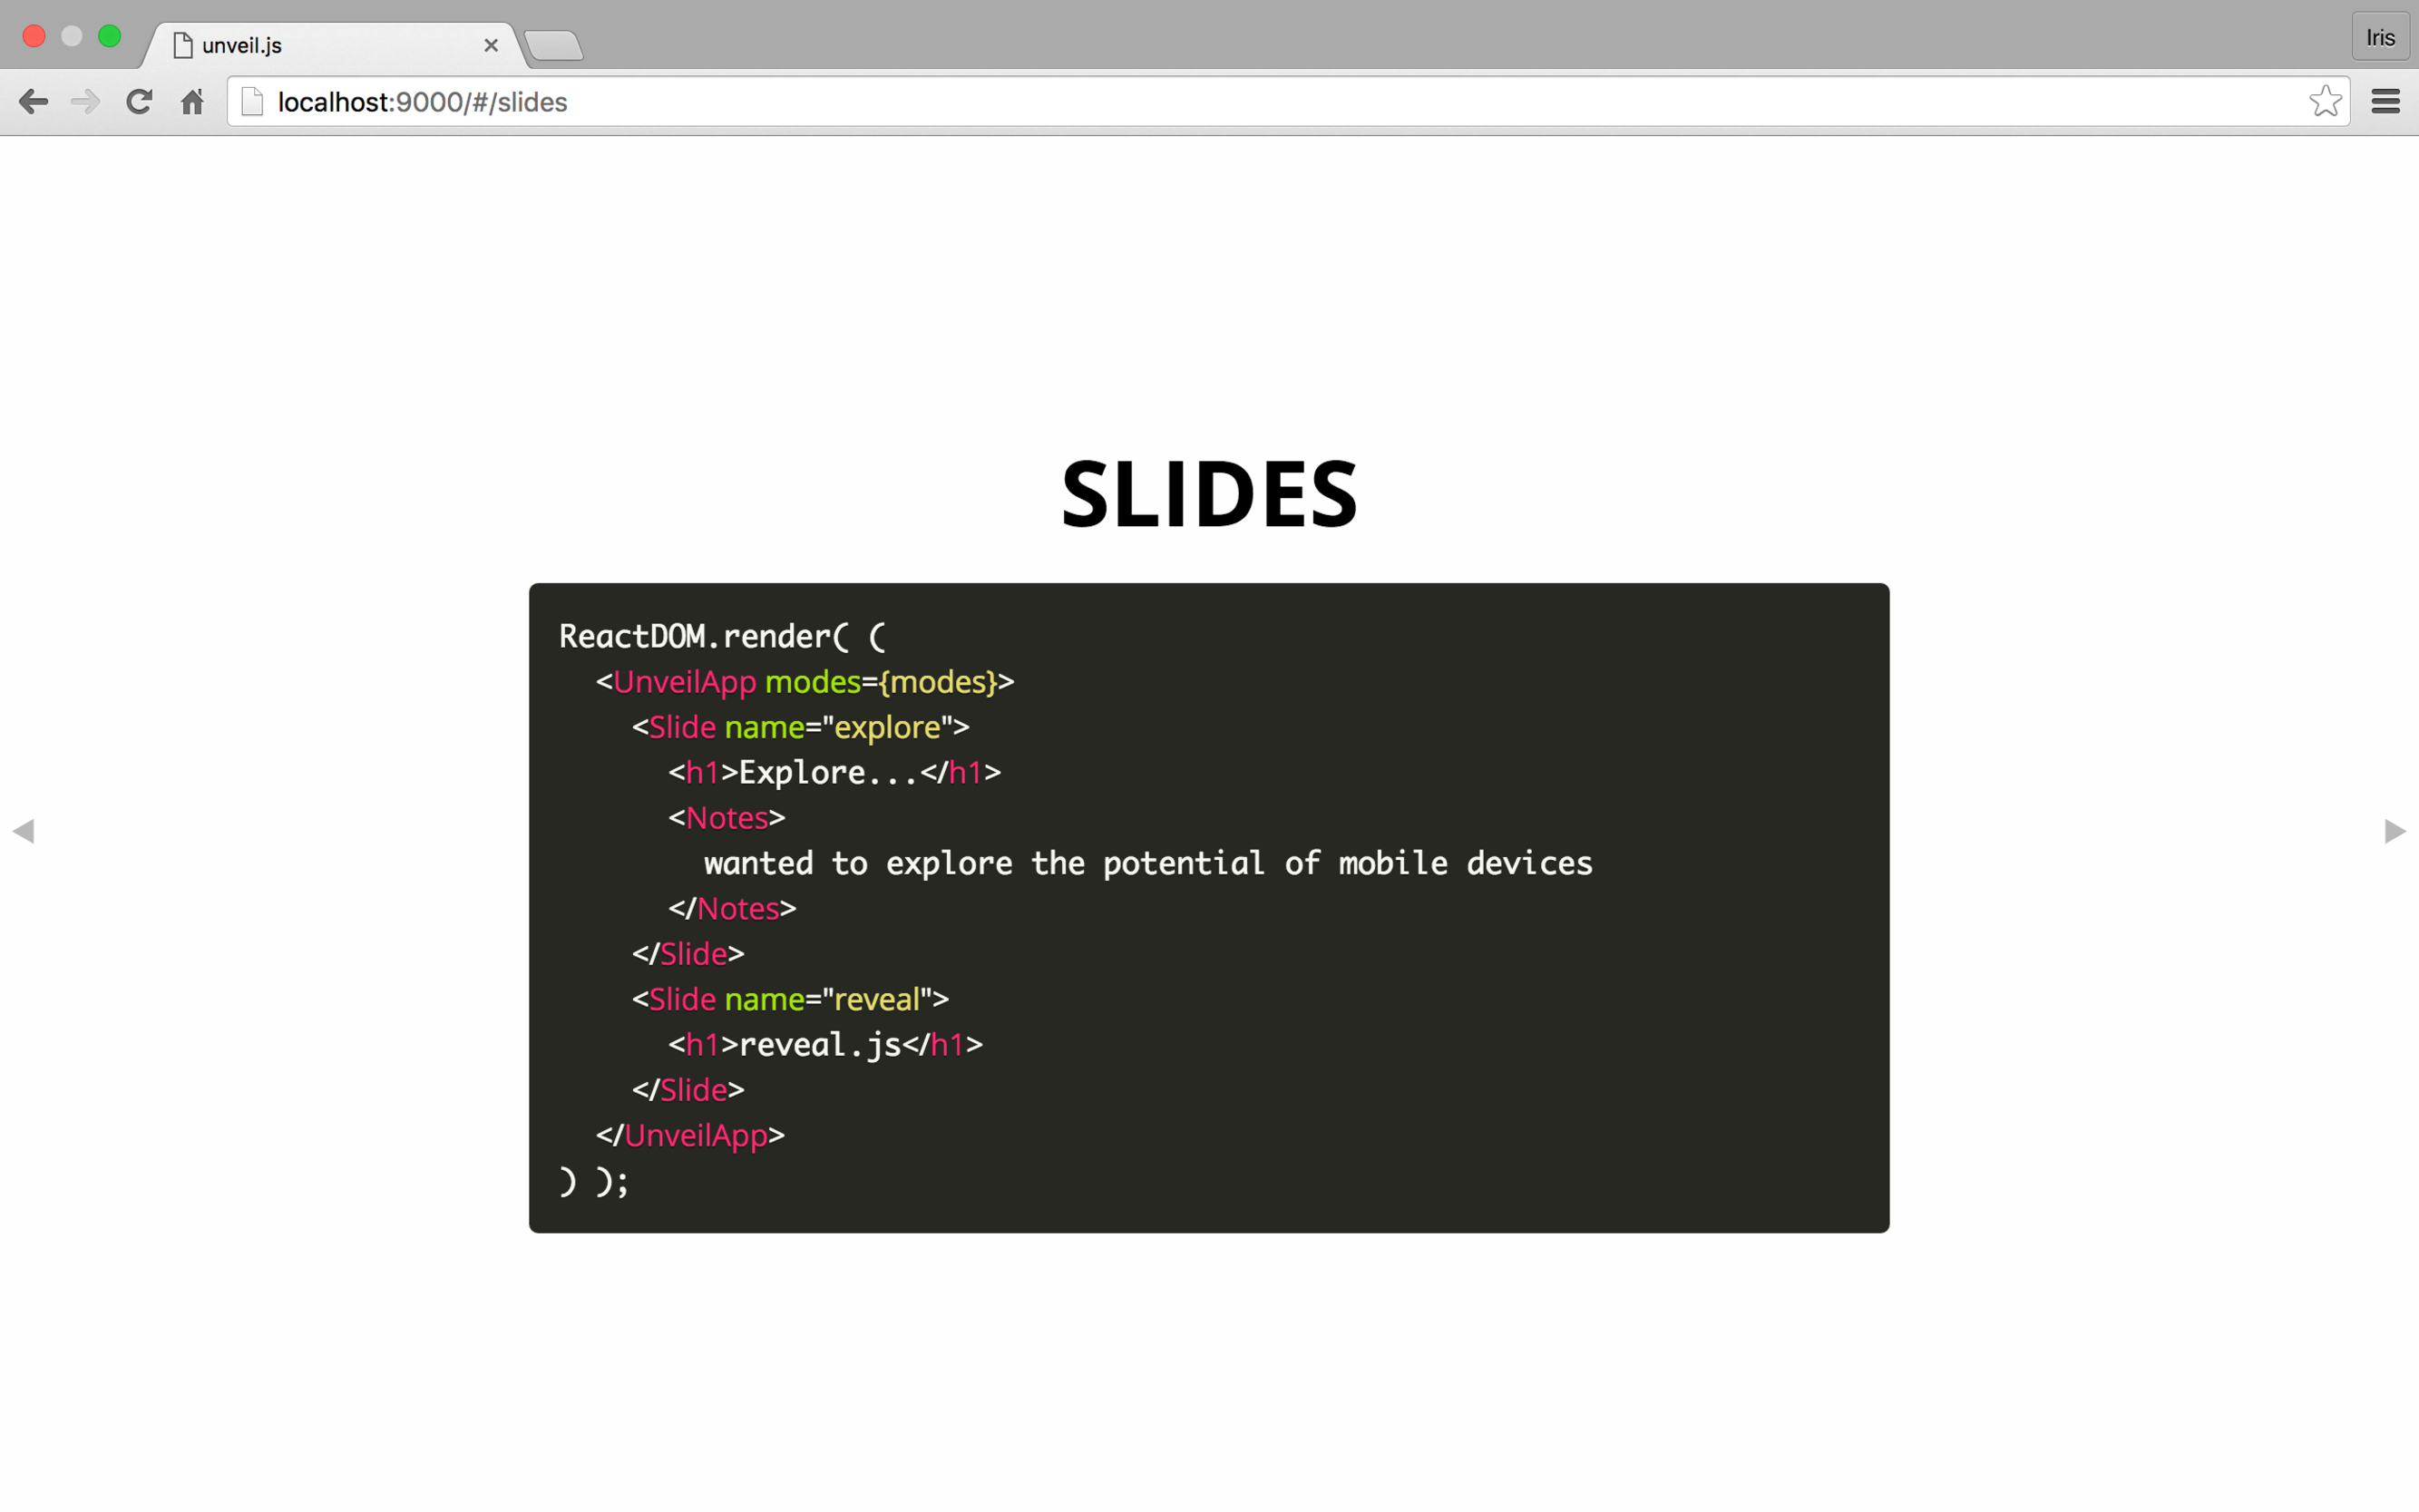
\includegraphics[width=0.5\textwidth]{unveil-screenshot}} &
%\FramePic{\includegraphics[width=0.3\textwidth]{unveil-screenshot-mobile}} \\
%(a) & (b) 
%\end{tabular}
%\caption{Screenshots from desktop (a) and mobile (b) view of unveil.js.}
%\label{fig:implementation-technologies-unveil-screenshots}
%\end{figure}

\begin{figure}
\centering
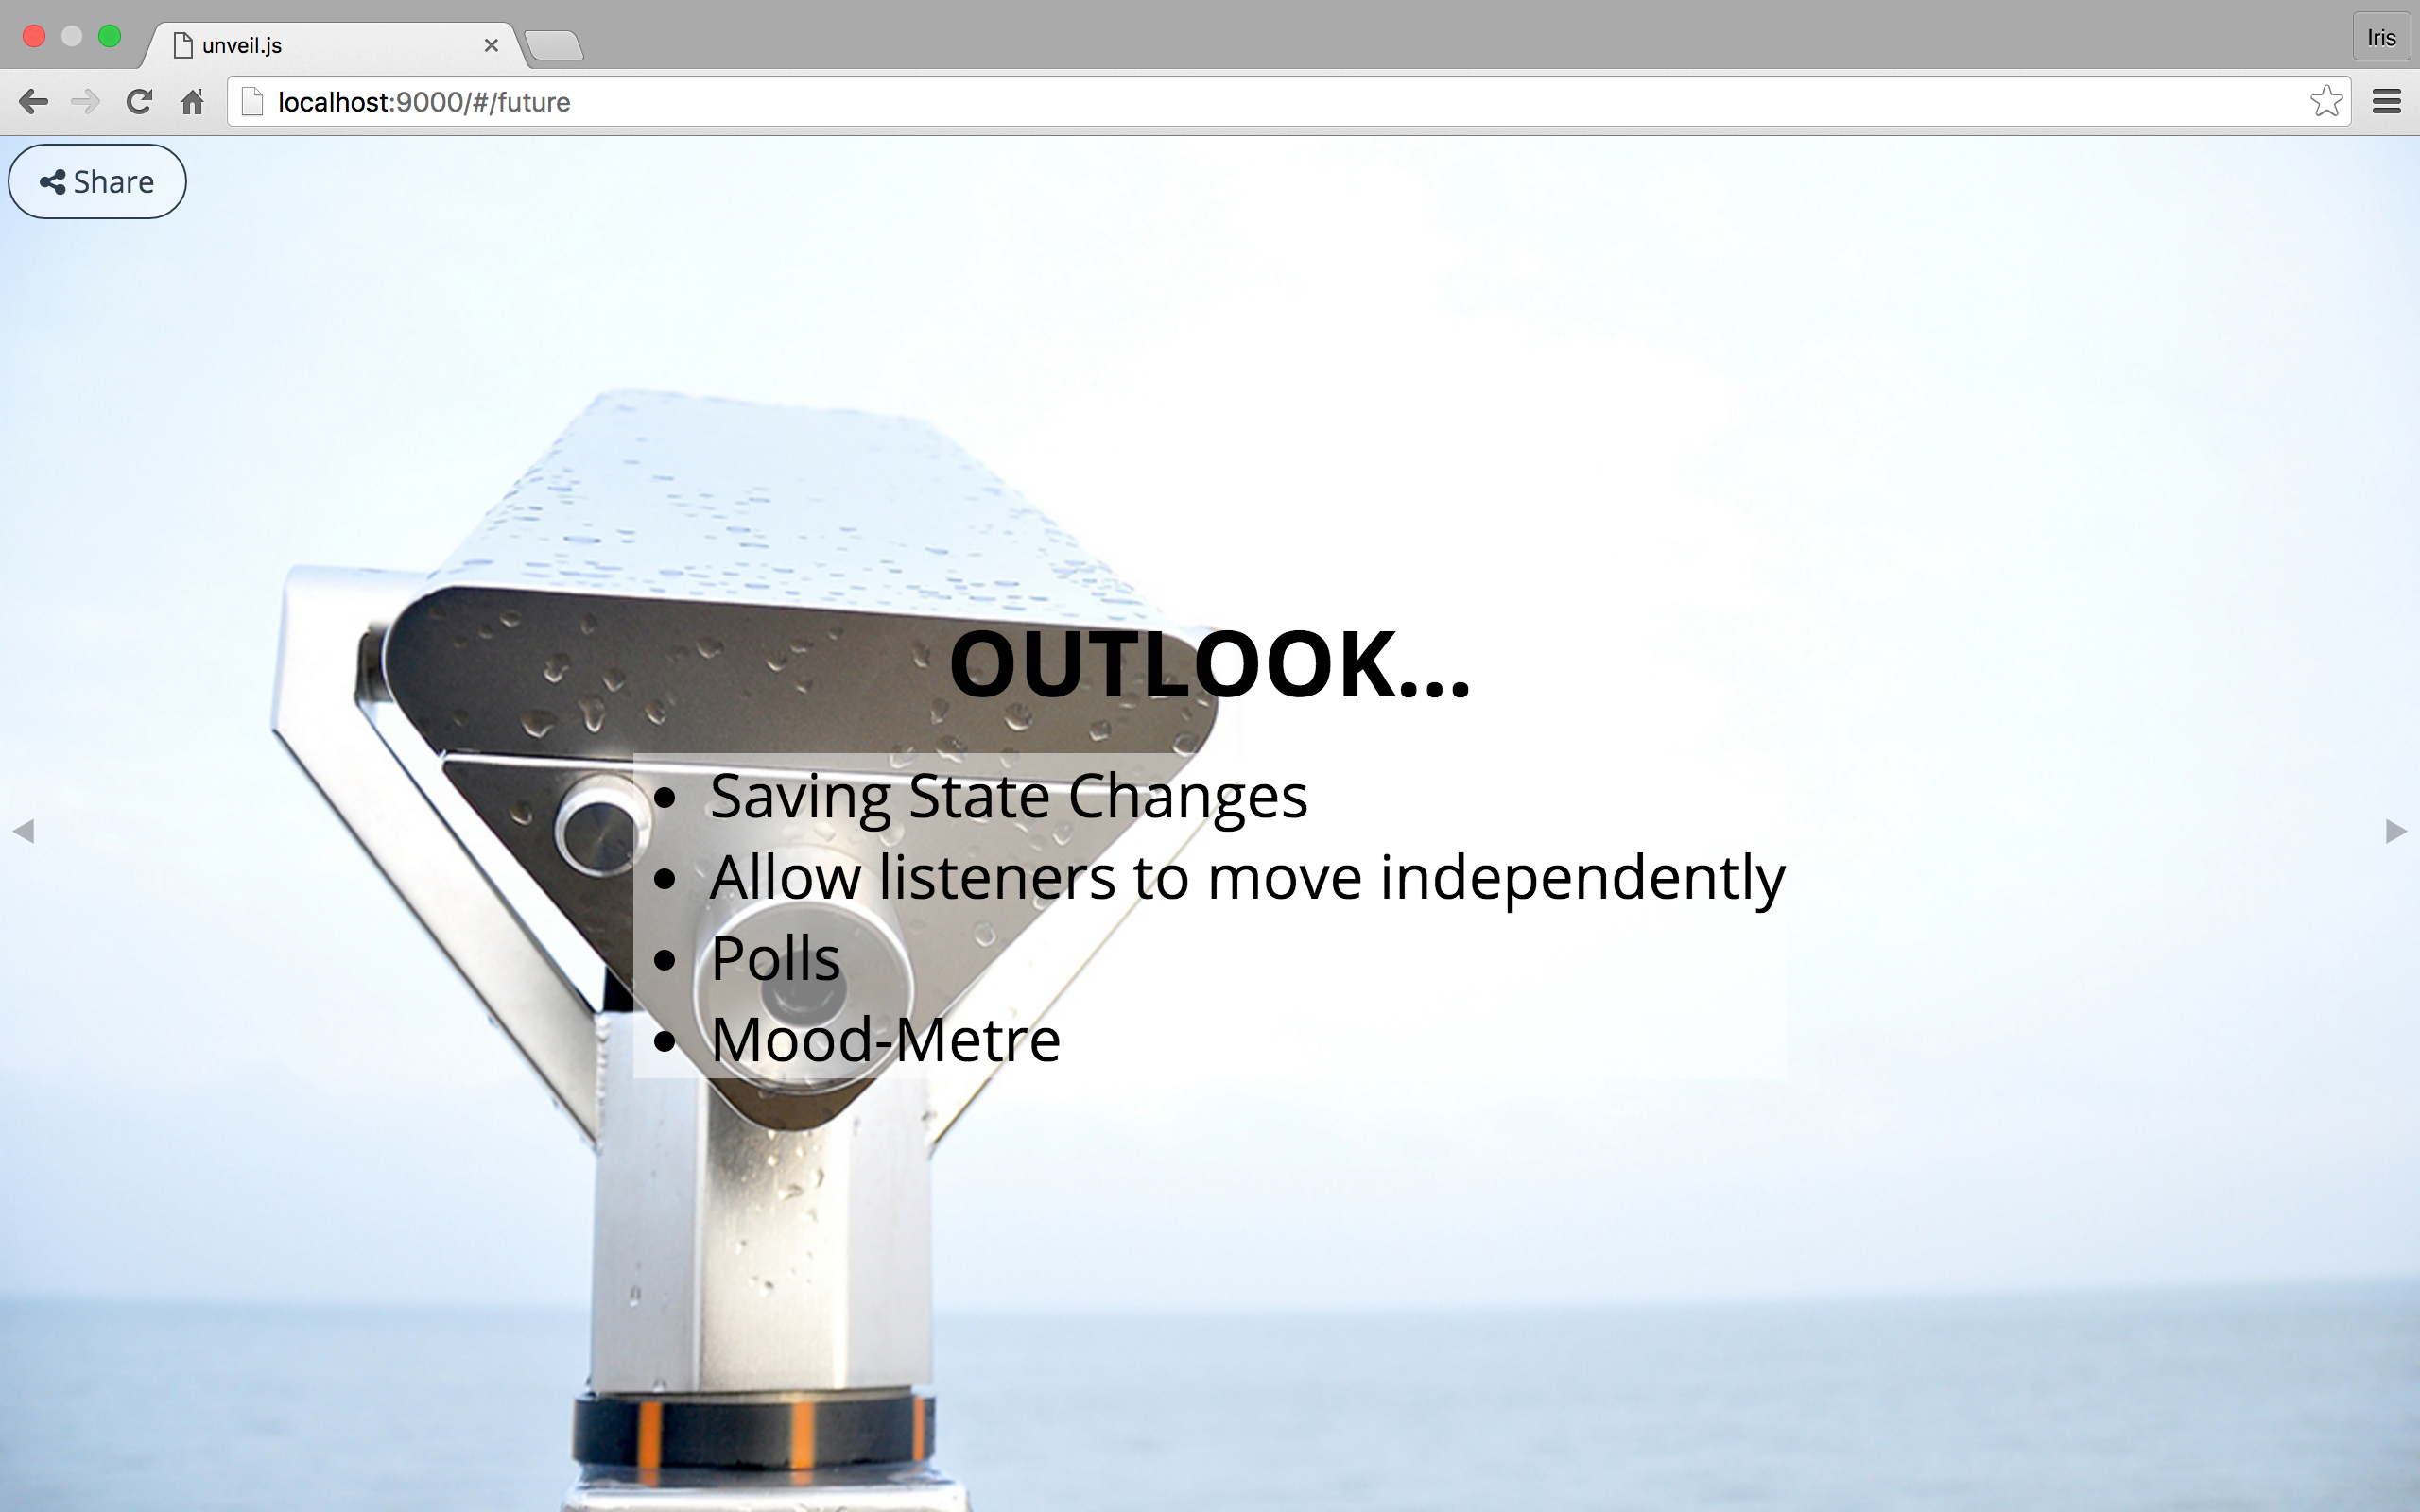
\includegraphics[width=0.65\textwidth]{presentation-screenshot}
\caption{Screenshot of an example slide with unveil.js, using interactive extensions discussed in section \ref{sec:implementation-interactive}.}
\label{fig:implementation-technologies-unveil-screenshots}
\end{figure}

Generally, unveil.js operates on a $2$-dimensional slide-space: Every slide can have a next and previous slide in $x$, as well as in $y$-direction. To generate the $y$ axis, slides can be nested in other slides. These slides have an optional unique name as well as an index in the slide-tree, which they are identified by. As shown in program \ref{prog:implementation-technologies-react}, slides are created inside the component \texttt{UnveilApp}, the core of unveil.js. This component configures and sets up the entire application based on optional configuration passed in as properties.
There are a few concepts unveil.js is built around to allow for extensibility and configurability, namely \emph{presenters}, \emph{controls} and \emph{modes}:
%
\begin{itemize}
\item \textbf{Presenters} define the way slides are rendered, e.g. show notes, upcoming slides or hide them.
\item \textbf{Controls} control a part of the application, e.g. navigating from one slide to the next using the arrow keys on the keyboard.
\item \textbf{Modes} are what allows a speaker to have a different presenter and controls from an audience member. Each mode defines its own presenter and set of controls, the mode is determined by the url query parameter \texttt{mode}.
\end{itemize}
This allows anybody using unveil.js to define new modes, presenters and controls and thereby extend the base library as they wish. A few of these are already defined, namely a default \texttt{Presenter}, \texttt{UIControls} to navigate using buttons, \texttt{KeyControls} to navigate using the keyboard and \texttt{TouchControls} to navigate with swipe-gestures on touch screens. In section \ref{sec:implementation-client}, modes for the audience (\emph{default}), the speaker (\emph{speaker}) and for use on the projection device (\emph{projector}) will be introduced.

For these controls and the entire presentation to be navigatable, \texttt{Un\-veil\-App} is responsible for the creation of two very important classes: \texttt{Router} and \texttt{Navigator}. These can be defined outside and passed into \texttt{UnveilApp} as properties, allowing users to customise their navigation logic.
%
The \texttt{Router} is the class handling everything connected to the current url. It receives the slide-tree and can compute the indices of a slide by its name and vice versa. Whenever the browser history changes, the router finds the corresponding slide-indices, computes an array of possible directions to go into from this slide and propagates the event to \texttt{UnveilApp}, which can then re-render the application.
\texttt{Navigator}, in turn, receives these directions and is responsible for the mapping of directions (\emph{left}, \emph{right}, \emph{up}, \emph{down}) to slide-indices. Controls know the navigator and can push new directions to the navigator subject, thus starting the navigation process described in detail in figure \ref{fig:implementation-technologies-unveil-navigation}.

\begin{figure}
\centering
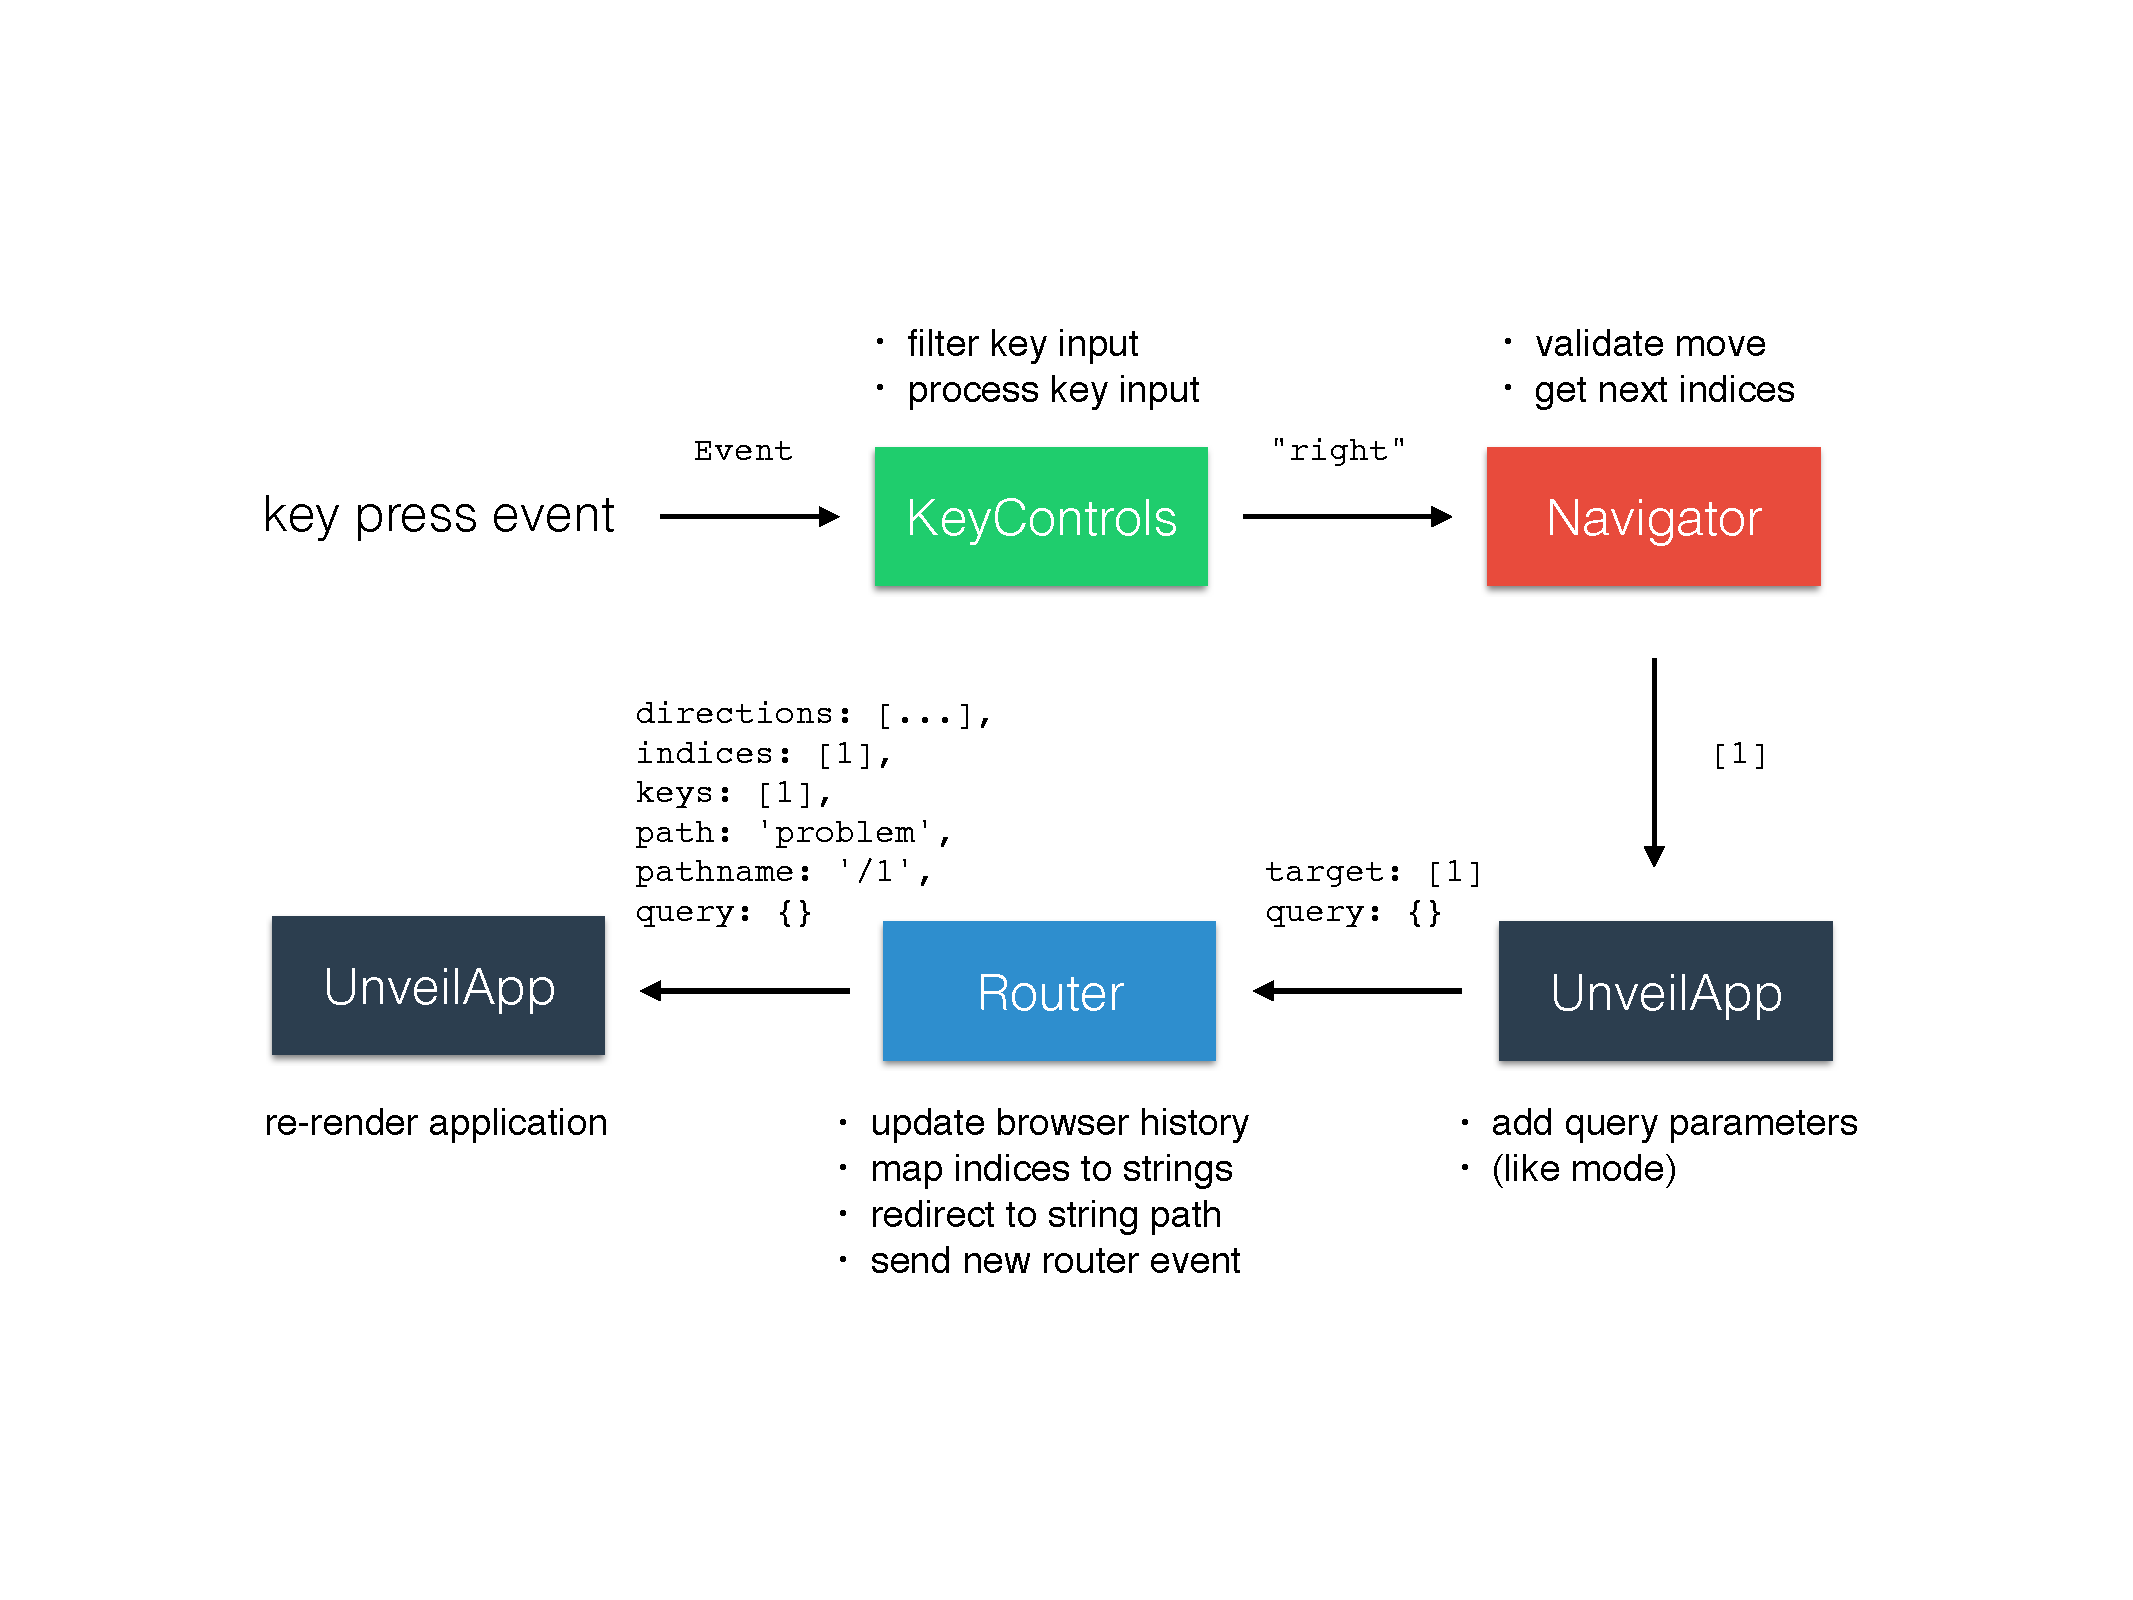
\includegraphics[width=.85\textwidth]{navigation}
\caption{Navigation pipeline from user's key press to re-render of the presentation. The monospaced text next to the arrows symbolises the data transmitted. \texttt{KeyControls} listen for key events and process them, to then send a navigation request to go \emph{right} to the \texttt{Navigator}. This component then maps the direction to the next slide's indices ($1$). \texttt{UnveilApp} then adds other information necessary for the \texttt{Router}, which then is responsible for updating the browser history, mapping the indices back to a human readable url and sending out a new router event. In the end \texttt{UnveilApp} receives this event and re-renders the presentation.}
\label{fig:implementation-technologies-unveil-navigation}
\end{figure}

%\subsection[socket.io]%
%             {socket.io%
%             \protect\footnote{\url{http://socket.io/}}}%
%\label{sec:implementation-architecture-socketio}
% problematic, talk about alternatives and problems in production, maybe even HTTP2
% e.g. safari conntection issues
% broadcasting functionality didn't quite work
% corporate firewalls can be a problem! big, in comparison to others

\section{Project Structure}
\label{sec:implementation-structure}
% A graphic explaining how the repos are built on top of each other would be great
% Which repos do I have and what do they include functionality-wise?
% explain why different repos and how they are all own npm packages that can easily be included in other projects

As the puropose of this project was not only to experiment with different ways of interacting with presentations using mobile devices, but also to create something worthwhile and contribute back to the vibrant open-source community, the project is enitrely open-source and separated into different repositories, which are all available on GitHub. These can be installed using npm, therefore allowing developers to rely only on the parts they really need.

\paragraph{Extended unveil.js:} As discussed in section \ref{sec:implementation-technologies-unveil}, the project is based on the library unveil.js. During the development of the project, certain parts of the base library did not offer the flexibility needed for easy extensibility and so several parts were adapted and new presentation logic was added. This happened in a fork of the original library, which will be examined in section \ref{sec:implementation-unveil}.

\paragraph{Network Synchronisation Layer:} The first library of direct importance for the interaction between speaker and audience through personal devices is \textit{unveil-network-sync}\footnote{\url{https://github.com/irisSchaffer/unveil-network-sync}}. This rather small library relies on unveil.js and is responsible for connecting the client and the server through web sockets and enables the synchronisation of the current slide displayed between speaker, audience and projector. The implementation of the features will be discussed in detail in section \ref{sec:implementation-network-sync}.

\paragraph{Interactive Extension:} As the name already suggests, this library is at the core of the present thesis: It includes a dedicated presenter for the speaker, implements the insertion of additional slides and subslides and by that allows the audience to share content with the presentation. The voting mechanism, as well as the creation of new votings on-the-fly, also live within this library. The repository, called \emph{unveil-interactive}\footnote{\url{https://github.com/irisSchaffer/unveil-interactive}} relies on unveil-network-sync for the socket-interaction. The interactive extension will be covered in section \ref{sec:implementation-interactive} of this chapter.

\paragraph{Server and Example Presentation:} The last repository connected to this thesis is \emph{unveil-client-server}\footnote{\url{https://github.com/irisSchaffer/unveil-client-server}}, which includes a simple server as well as a real-world example of a presentation, which was used in the intermediate thesis project presentation as part of the Interactive Media course IM690, on the 2\textsuperscript{nd}\xspace of February, 2016. In this chapter, a whole section was dedicated to the server (\ref{sec:implementation-server}), as well as to the example application (\ref{sec:implementation-client}), to separate concerns a bit more clearly and be able to conclude with a demonstration of how all parts discussed earlier play together in a final presentation.

\section{Extended unveil.js}
\label{sec:implementation-unveil}
% Add screenshots from biiiiiiig screen :)
The biggest adaptions and additions were necessary in the main component \texttt{UnveilApp}. A state subject was added to allow all components in the presentation to interact with the application. This subject receives an event with type and data and depending on this type starts a certain state change. Two of these state events are the \texttt{state/navigation:enable} and \texttt{state/navigation:disable} events, which set a state-variable \texttt{navigatable} to true or false. This variable is used in the controls to determine navigatability, therefore making it possible to keep the audience locked to a slide, e.g. during votings.
To make it possible for the audience to add subslides, as well as to dynamically add votings on-the-fly, another event is \texttt{state/slide:add}. It includes what slide to add (content), how (subslide or main slide) and where (under or after which slide). On occurence of this event, the slide-tree has to be re-built, the router and navigator re-started and the whole presentation re-rendered, which the library also had to be prepared for.

\begin{figure}
\centering
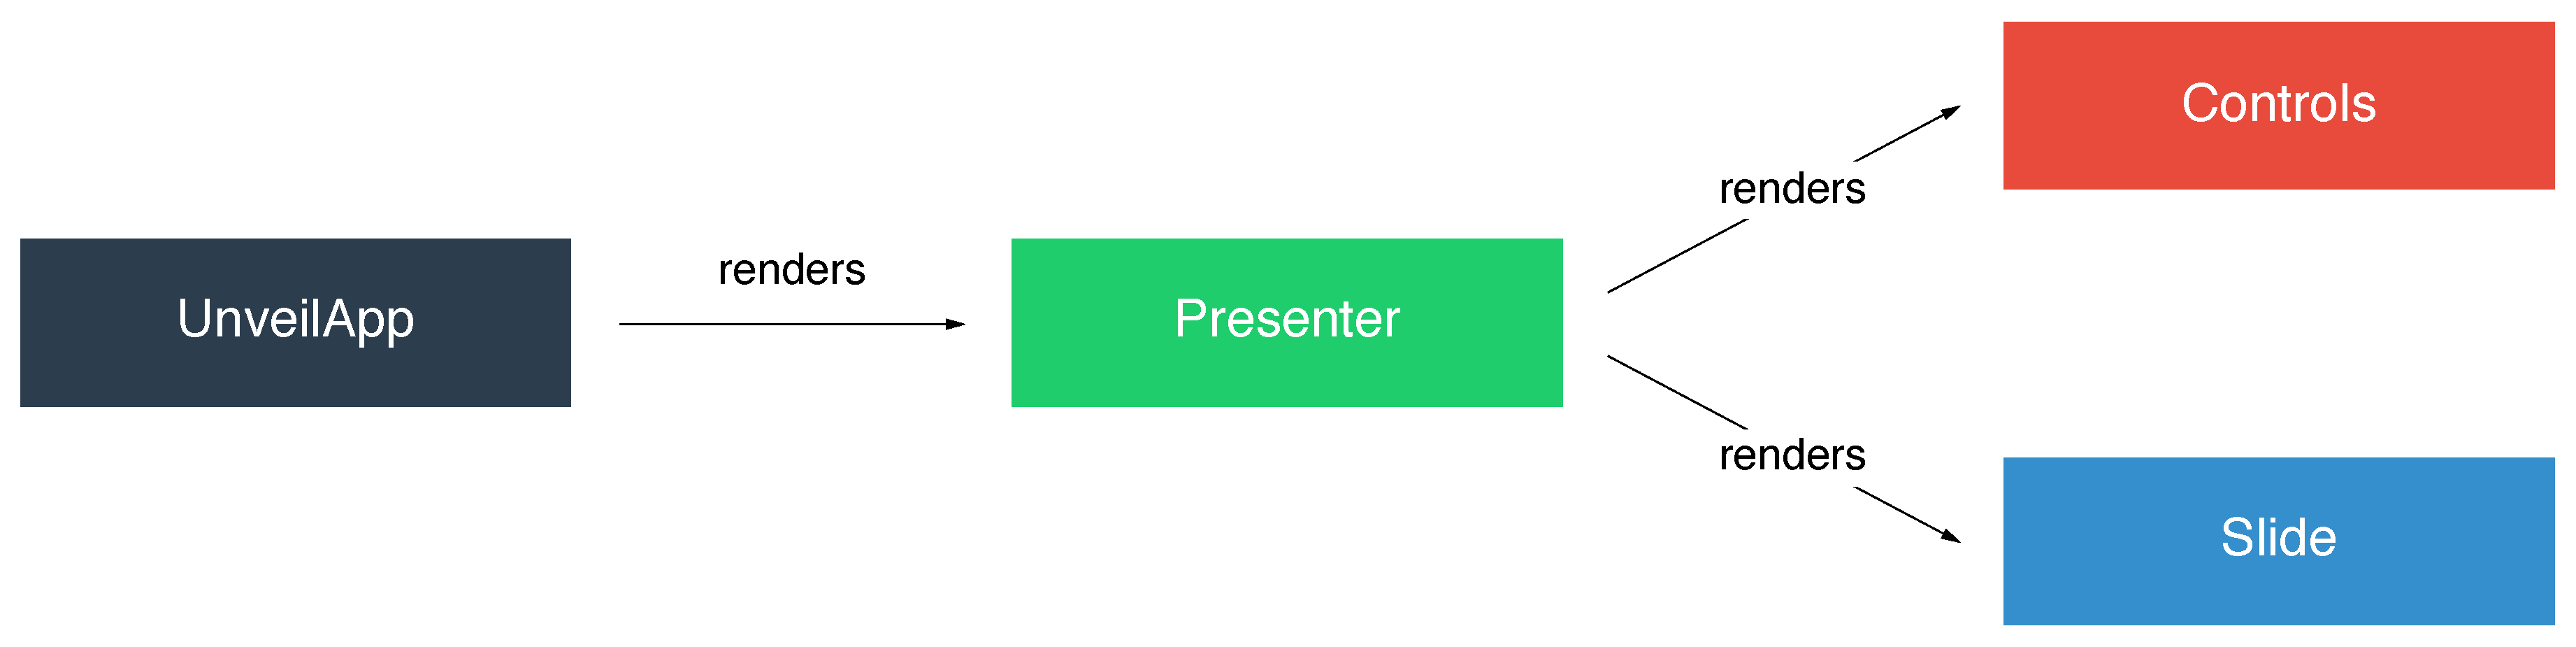
\includegraphics[width=.5\textwidth]{render-pipeline}
\caption{Overview over the render-flow of the application in the extended version of unveil.js. \texttt{UnveilApp} renders the presenter, which then takes care of rendering the (current) slide and all controls.}
\label{fig:implementation-unveil-render-pipeline}
\end{figure}

Another adaption in \texttt{UnveilApp} is the introduction of the \texttt{context} object: Additionally to state and properties, there is a third way of communicating between components in React, called \emph{context}. Instead of having to pass properties from one nested component to the other, every child component can access the context of its parents. The navigator, needed in the controls, was formerly passed from \texttt{UnveilApp} to the controls through several layers. Using context, \texttt{UnveilApp} now defines a number of different variables which are available through context, including current slide and router state, navigator, mode and the state subject discussed in the last paragraph. This makes it easy for new controls and presenters to access the data they need without other layers knowing about them or having to define them.
This adaption was partly due to a change in the render hierarchy: Formerly, \texttt{UnveilApp} itself rendered the presenter (which rendered the current slide) and the controls. However, the presenter needs to be able to also control the rendering of controls (see figure \ref{fig:implementation-unveil-render-pipeline}), adding another layer between the rendering of controls and \texttt{UnveilApp}.

Another part that was added to the unveil.js base library is the \texttt{Notes} component. It allows adding speaker notes to each slide (see program \ref{prog:implementation-technologies-react}). These, however, are not rendered by the slide, but by the presenter, as will be shown in section \ref{sec:implementation-interactive}. One more important new feature is the possibility to configure the next slide in a certain direction (left/right/up/down) and therefore allow for jumping into different branches of the presentation, thus making a presentation even more interactive. The following code, for example
%
\begin{JsCode}
  <Slide name="start" left={[0]}>
    ...
  </Slide>
\end{JsCode}
%
means a navigation \emph{left} (left arrow key pressed, swipe left etc.) will not go to the previous slide defined in the slide-tree, but rather jump to the first slide (of index $0$).


\section{Network Synchronisation Layer}
\label{sec:implementation-network-sync}
% Mention problems with socket io here! --> Corporate firewalls can block socket io entirely, etc.
As mentioned before, the network synchronisation layer is responsible for the communcation between server and client using web sockets. These are created with socket.io, a library which also provides fallbacks for browsers that do not support web sockets yet. However, this library also has a few drawbacks, especially when it comes to corporate networks. As Rob Britton describes in \cite{socketio-problems}, socket.io seems to have problems getting through firewalls and can be blocked by some anti virus software.
Because mobile browser support is essential for this project, I decided to still use this library.

The setup of the socket is simple: one helper function, called \texttt{createSocket} is called in the main entry point of the application to configure which server to connect to:
%
\begin{JsCode}
import { createSocket } from 'unveil-network-sync'
createSocket('46.101.166.172:9000')
\end{JsCode}
%
This function creates the socket and returns it as a singleton, so every component uses the same connection. To make importing even easier, there is another helper, called \texttt{SocketIO} which dan be importet directly and internally calls \texttt{createSocket} to retrieve the singleton:
%
\begin{JsCode}
import { SocketIO } from 'unveil-network-sync'
\end{JsCode}
%

These sockets can then be used to listen to events or to emit them (see program \ref{prog:implementation-network-sync-navigation-receiver}) Like the state subject events, the socket.io events used in this library follow the naming convention of scoping the object targeted in by the event separated by slashes, followed by a colon and the name of the action, e.g. \texttt{state:change} or \texttt{state/slide/voting:start}.

\begin{program}
\caption{Shortened version of \texttt{NavigationReceiver}. First the inherited context properties are set up, then an observable waiting for \texttt{state:change} events from the socket is created. If the incoming request is not the currently displayed slide, the navigator will be pushed a new value.}
\label{prog:implementation-network-sync-navigation-receiver}
\begin{JsCode}
// imports...

export default class NavigationReceiver extends React.Component {
  static contextTypes = {
    navigator:   React.PropTypes.object.isRequired,
    routerState: React.PropTypes.object.isRequired
  }

  componentDidMount () {
    this.observable = Observable.fromEvent(SocketIO, 'state:change')
      .filter((e) => !this.context.routerState.indices.equals(e))
      .subscribe(this.props.navigator.next)
  }
  ...
}
\end{JsCode}
\end{program}
%
The second responisbilty of this library is synchronising the navigation state of the presentation between speaker and audience. To do this, two controls, \texttt{NavigationSender} and \texttt{NavigationReceiver} were implemented. As the names already say, the sender broadcasts the state update, while the receiver is waiting for state updates and starts the navigation process. The latter is used in all modes (default, speaker and projector), whereas the sender is only added to the speaker mode. To make sure the sender does not end up in an infinite loop of sending and receiving its own state changes, the last received state is stored and only navigation events going to a different slide are processed further.

This mechanism, though relatively simple, already enables the audience to follow the presentation, the speaker to use his/her phone as a remote control and any number of projectors to be controlled by the speaker.

\section{Interactive Extension}
\label{sec:implementation-interactive}
The interactive library includes several parts which will be discussed here: a speaker presenter (section \ref{sec:implementation-interactive-speaker-presenter}) as well as different components connected to sharing media (section \ref{sec:implementation-interactive-media}) and voting (section \ref{sec:implementation-interactive-voting}). Additionally controls handling the \texttt{state:initial} event were implemented to redirect new listeners to the current slide in the presentation.

\subsection{Speaker Presenter}
\label{sec:implementation-interactive-speaker-presenter}

The speaker presenter, like the normal presenter, is responsible for rendering controls and slides. In speaker mode, where this presenter is used, notes as well as the upcoming slides (right and down) are also shown (see figure \ref{fig:implementation-interactive-speaker-presenter}).
This means the presenter has to find these next slides, using the router's information about the navigatable directions, and render them in a designated area. To make the presenter view usable on mobile devices, special attention was paid to mobile stylesheets (see figure \ref{fig:implementation-interactive-mobile} (b)). This ensures that everything is big enough to be readable and all buttons are clickable.

\begin{figure}
\centering
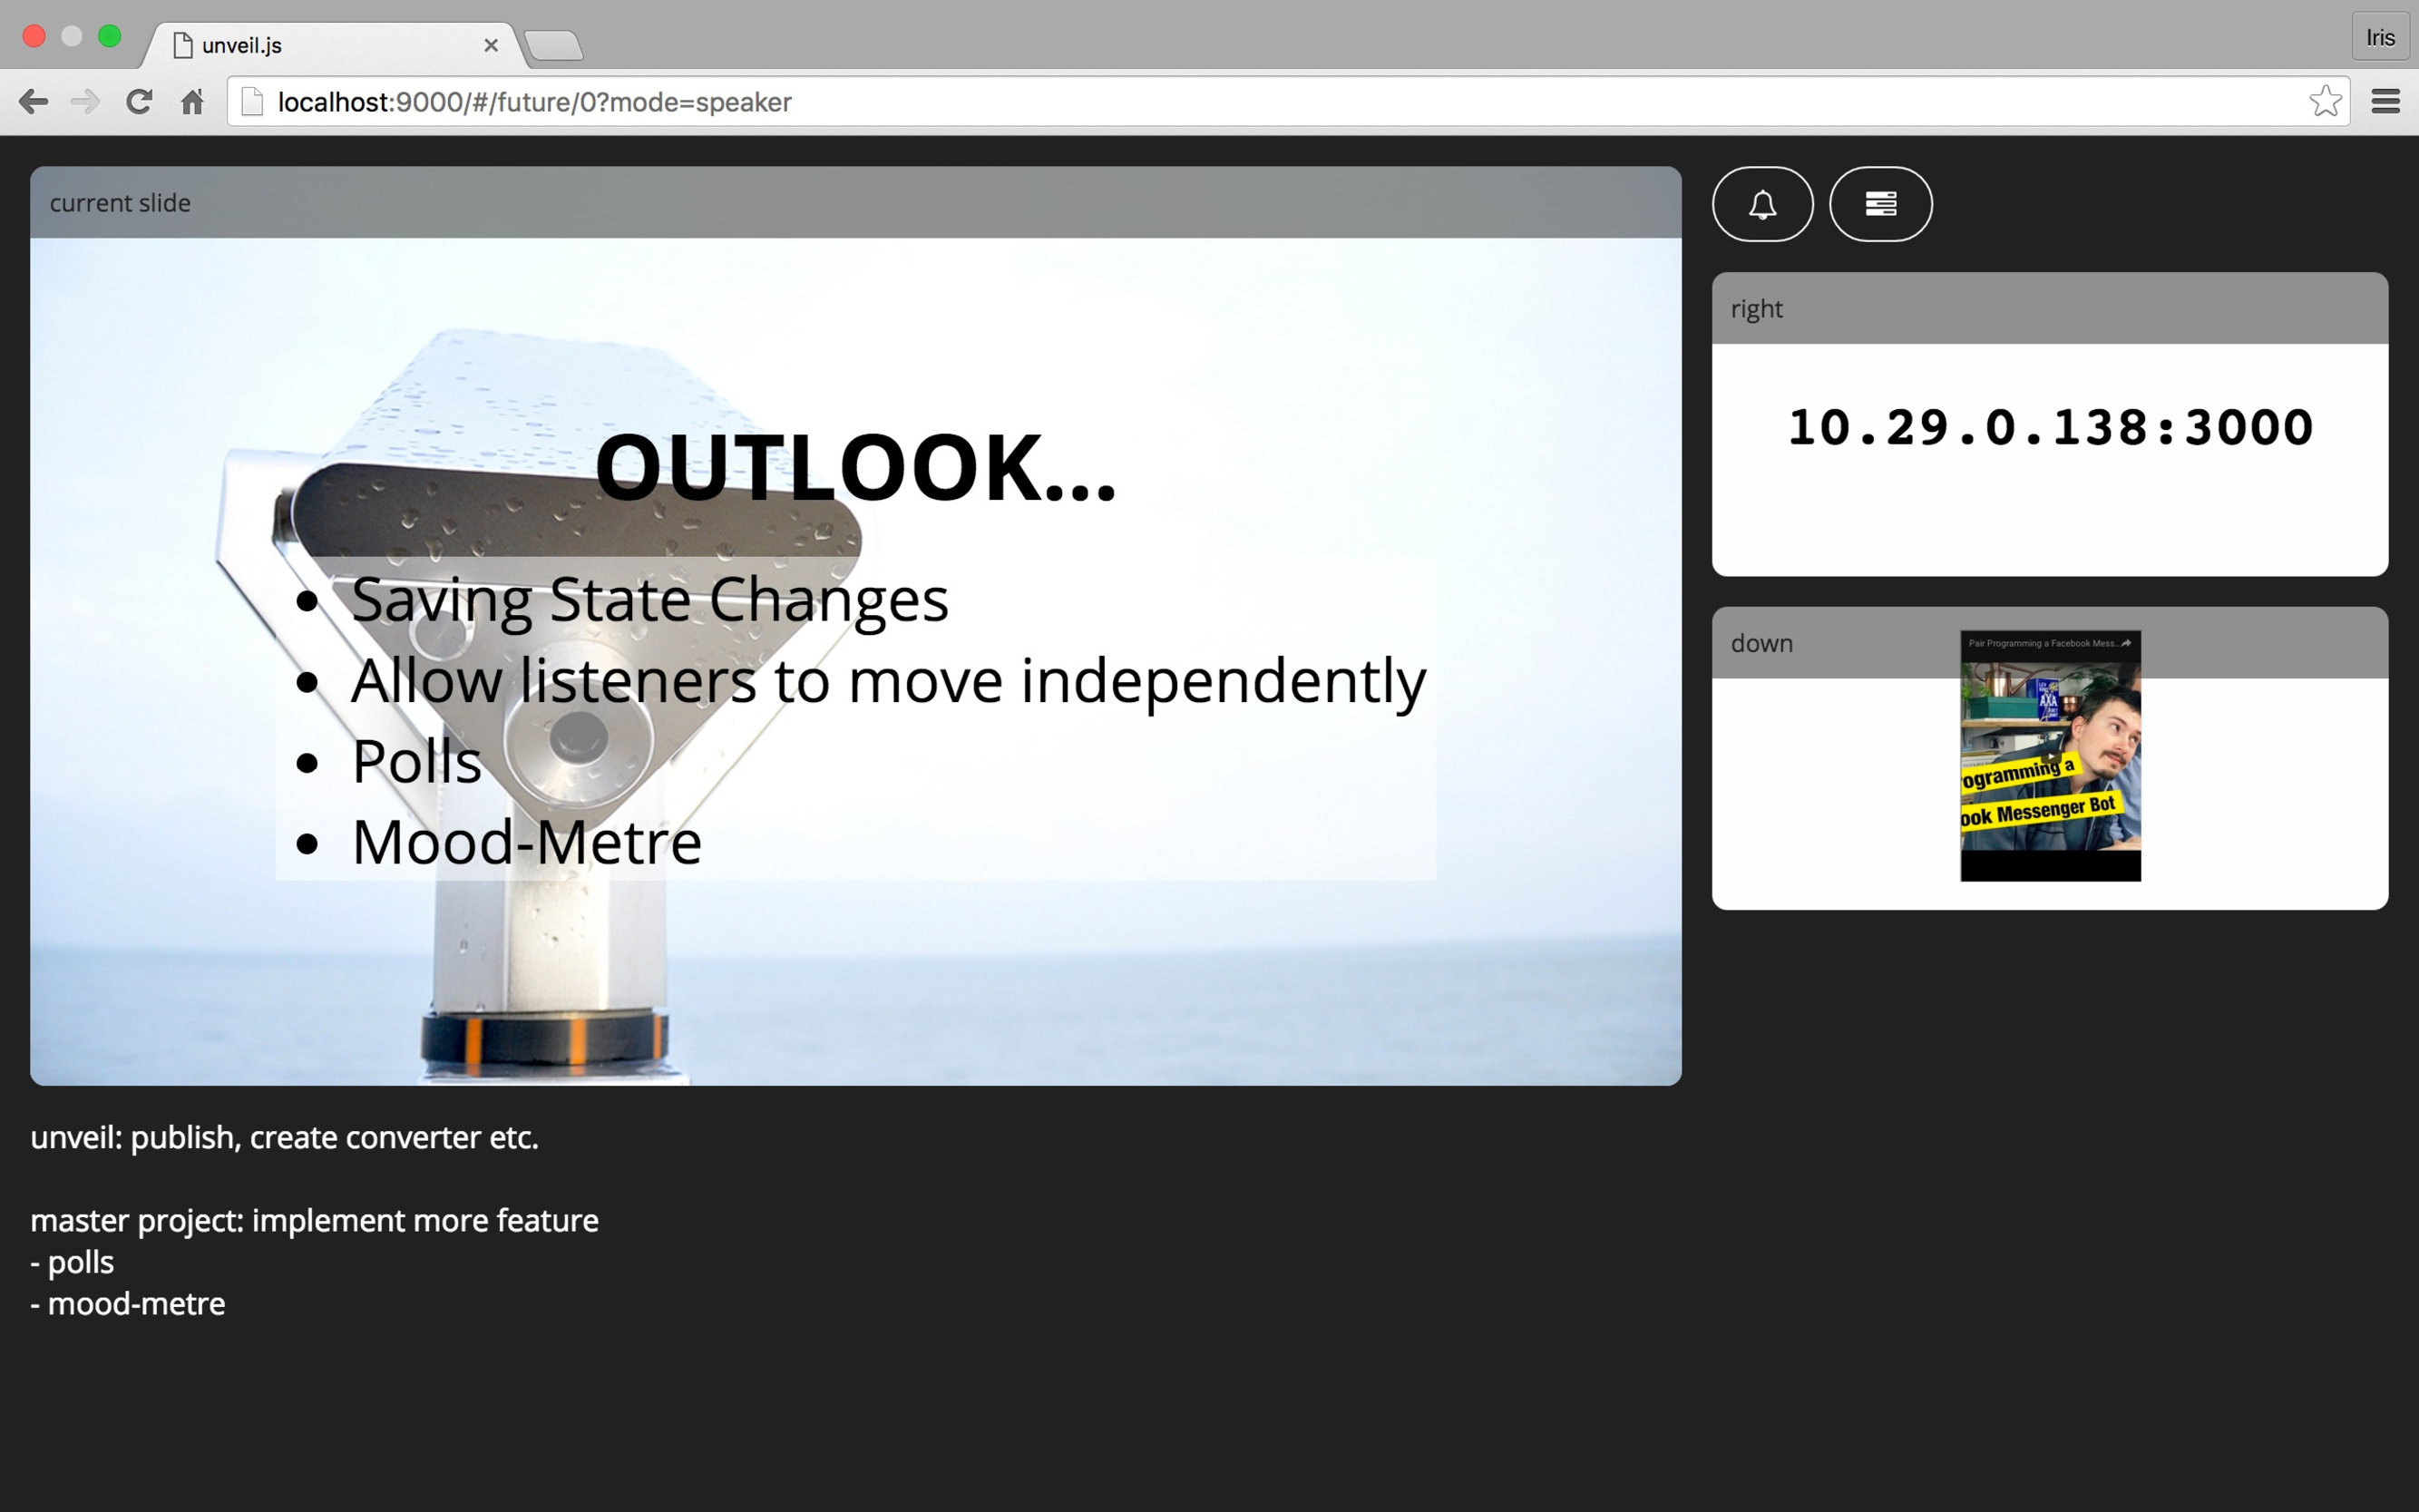
\includegraphics[width=.65\textwidth]{media-accepted-screenshot}
\caption{Screenshot of the speaker presenter with the current main slide, the upcoming slide to the right, available actions (muting and adding votings) and speaker notes.}
\label{fig:implementation-interactive-speaker-presenter}
\end{figure}

\begin{figure}
\centering\small
\begin{tabular}{cccc}
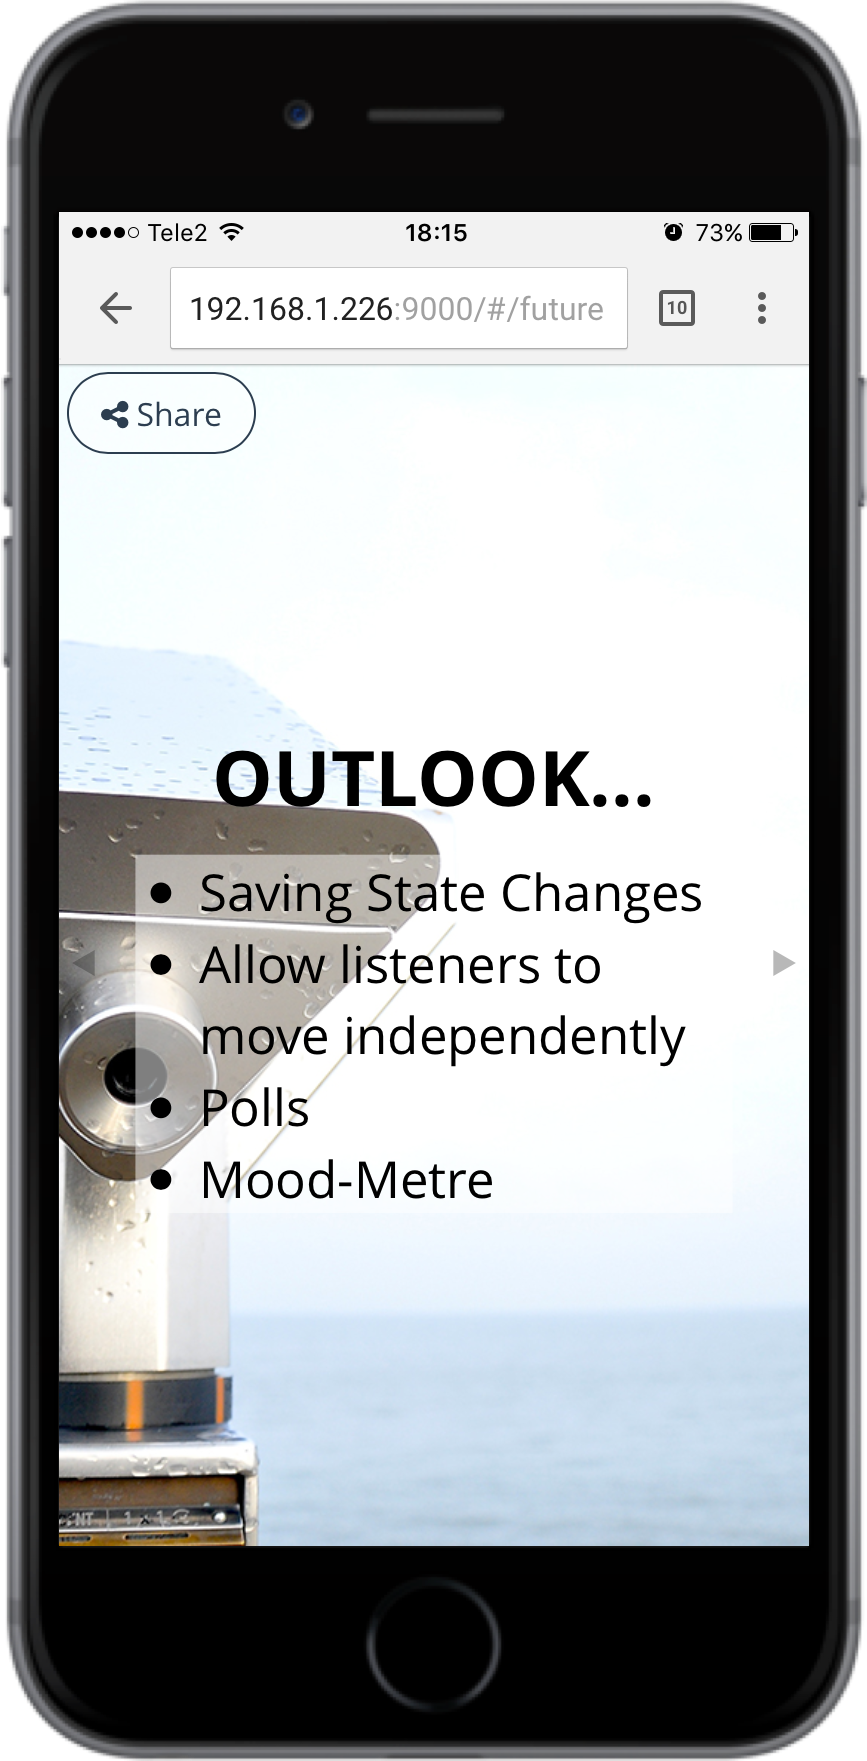
\includegraphics[width=.2\textwidth]{presentation-screenshot-mobile} &
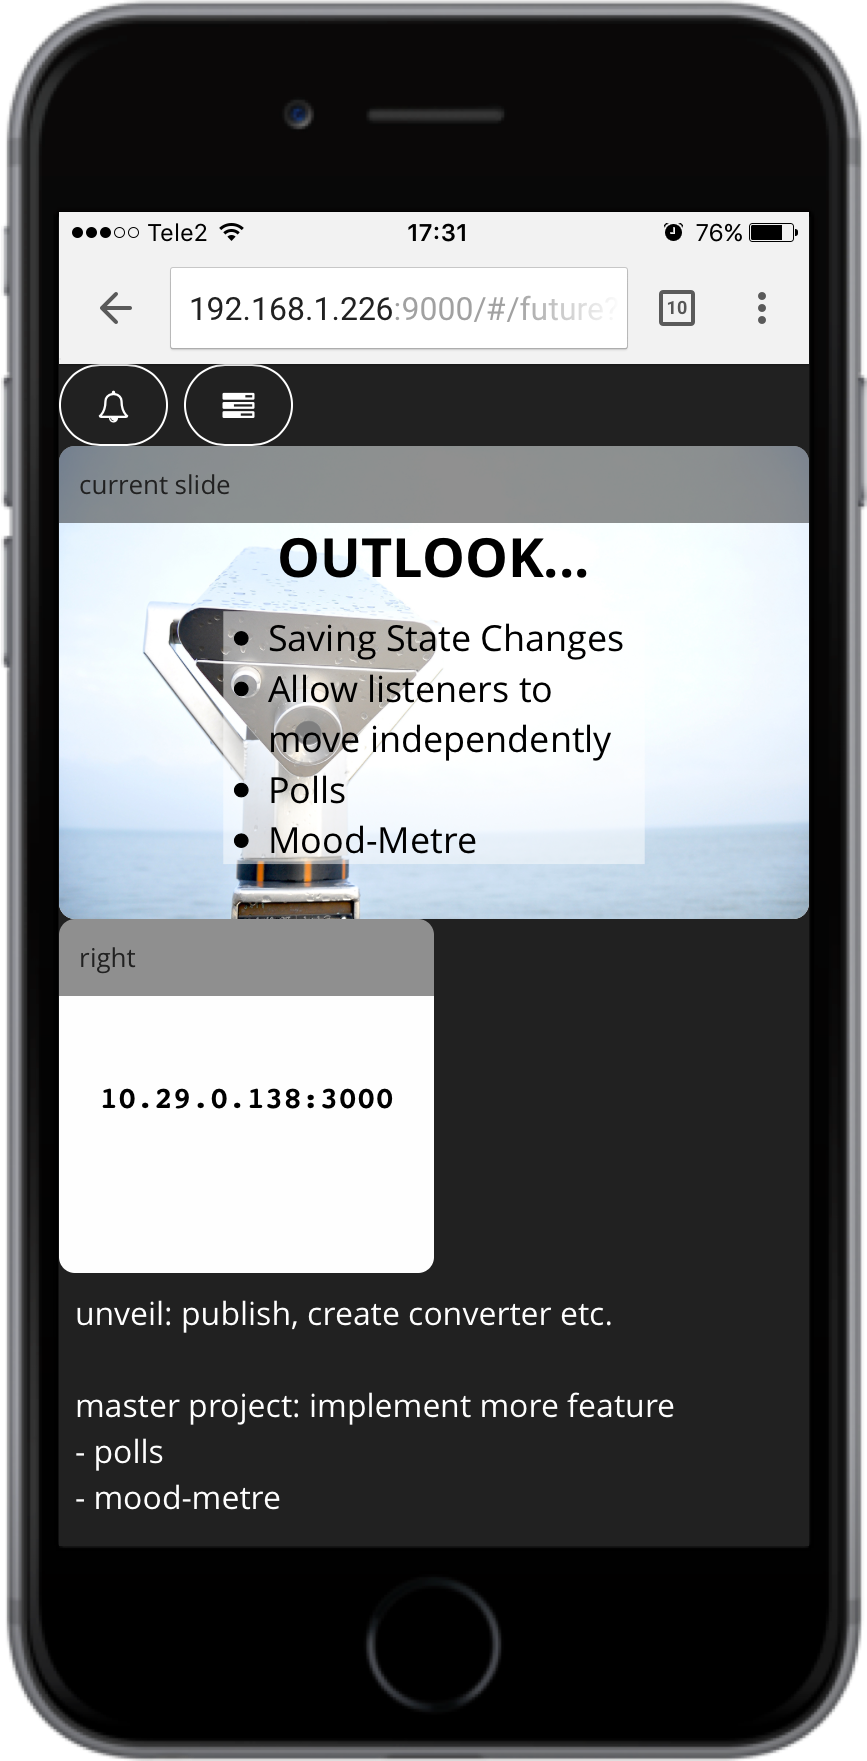
\includegraphics[width=.2\textwidth]{speaker-presenter-screenshot-mobile} &
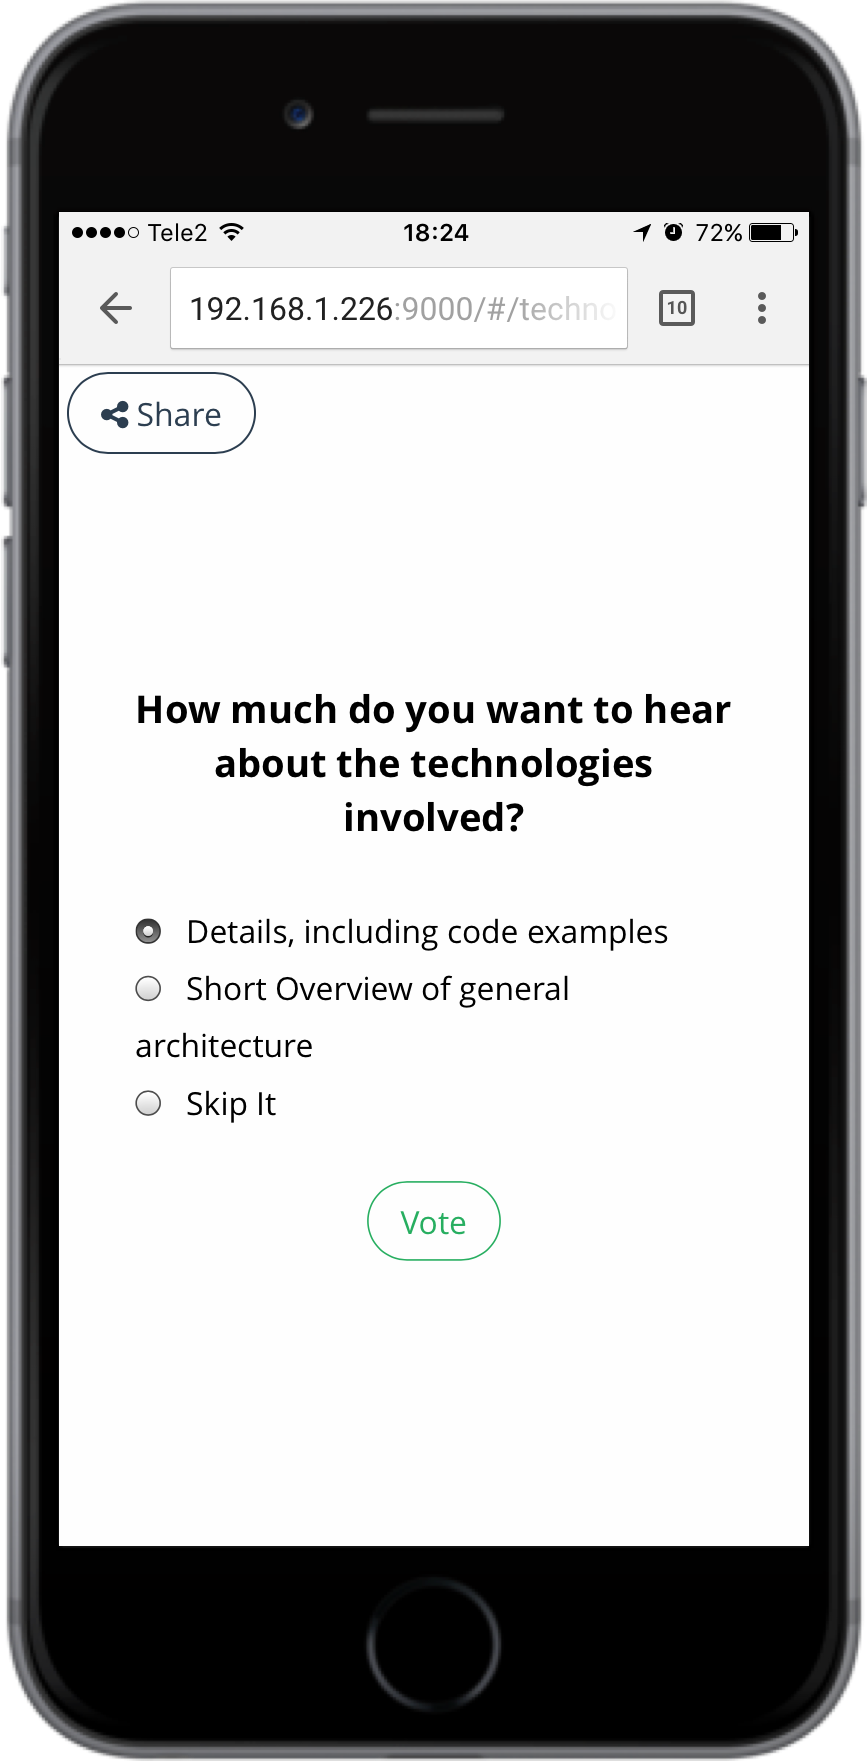
\includegraphics[width=.2\textwidth]{voting-screenshot-mobile} &
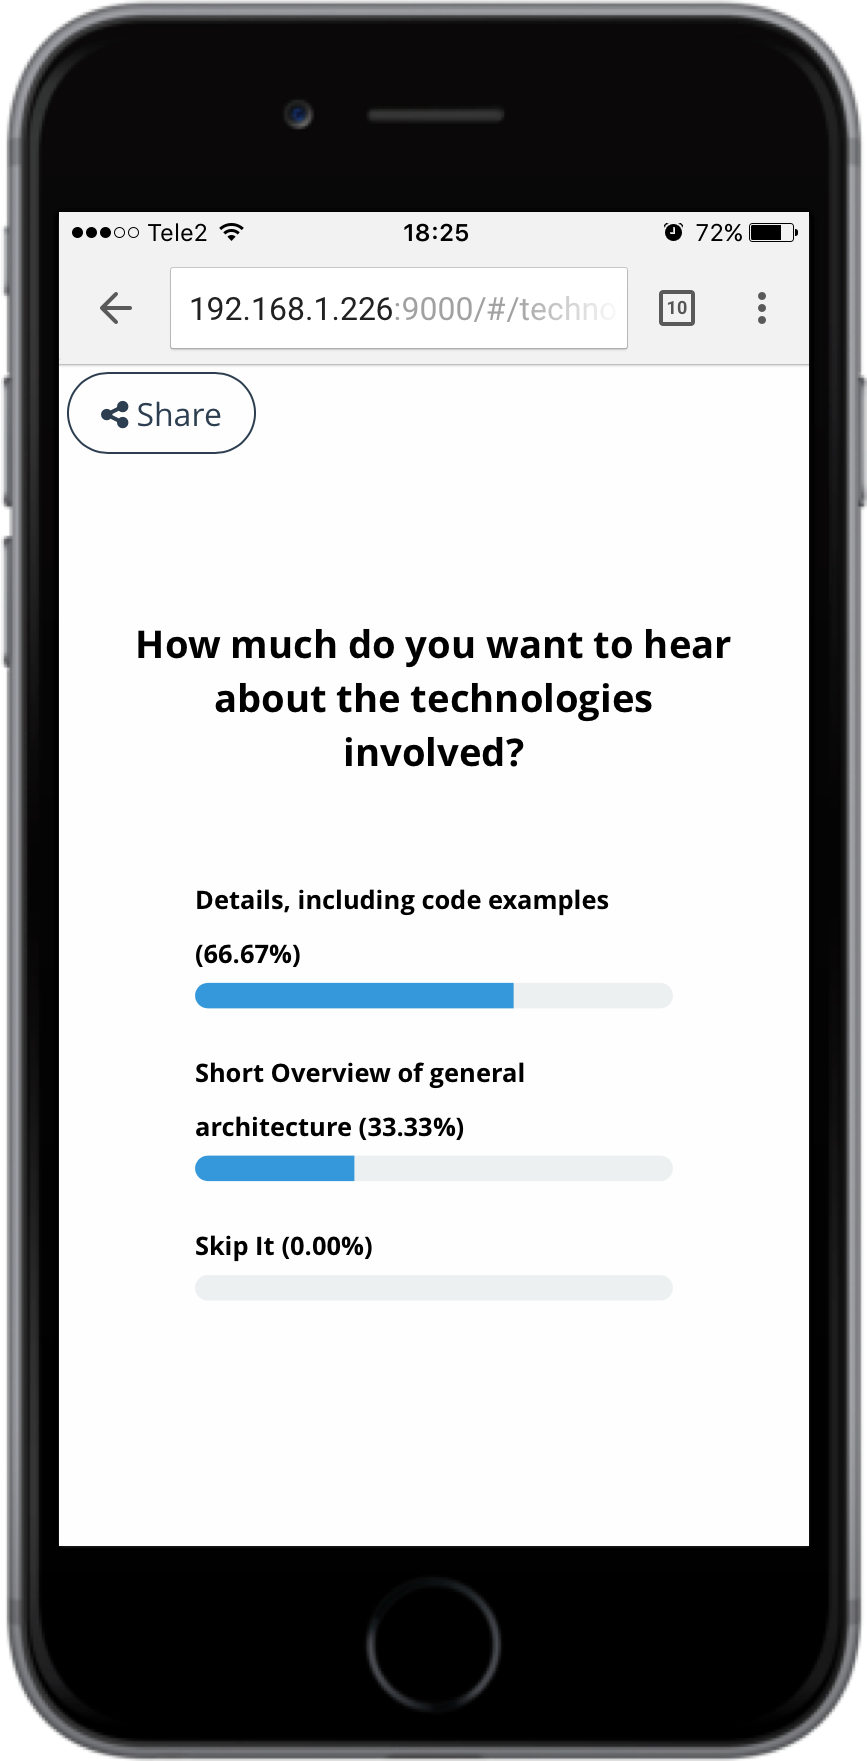
\includegraphics[width=.2\textwidth]{voting-results-screenshot-mobile} \\
(a) & (b) & (c) & (d)
\end{tabular}
\caption{Mobile view of a presentation slide in (a) default mode and (b) speaker mode as well as (c) voting view before voting and (d) voting view after voting. Mind the share button in the left upper corner in (a) as well as the buttons to mute content requests and create votings in (b).}
\label{fig:implementation-interactive-mobile}
\end{figure}

\subsection{Media}
\label{sec:implementation-interactive-media}
Another responsibility of the interactive extension is the possibility for audience members to share content with the presentation. For this to work, three different controls were created: \texttt{MediaSender}, \texttt{MediaReceiver} and \texttt{MediaAcceptor}. The sender is used in the default mode so users can share their content (see figure \ref{fig:implementation-interactive-media} (a)), the acceptor is enabled in speaker mode, to accept or reject incoming media (see figure \ref{fig:implementation-interactive-media} (b)) and the receiver in the end handles the creation of a new slide if the content was accepted and is therefore necessary in all modes. As incoming content requests could disrupt the presentation flow and distract the speaker, an option to mute the requests was built into the application. If the \emph{do not disturb} mode is turned on, slides will silently be added as subslides, without causing the acceptor modal to open. This way the audience' additions can be re-visited after the end of the presentation. Generally, this feature can be used to either post a link to an interesting picture, website or even youtube video, or also as text input, for example to add a comment or a question regarding a certain slide. This works through the introduction of the presentation components \texttt{Media} and \texttt{IFrame}, which, depending on the shared content, render an image-tag, blockquote or IFrame. The differentiation of these is carried out with regular expressions, as the following to check if the content is the link to an image:
\begin{JsCode}
isImg (str) {
  let imgRegex = new RegExp(/\.(jpe?g|png|gif|bmp)$/i)
  return imgRegex.test(str)
}
\end{JsCode}

As far as the implementation of the controls is concerned, these ones are the first ones discussed in the present thesis makeing use of the \texttt{render()} method. It is used to output the \emph{share} button in the left upper corner in default mode (see figure \ref{fig:implementation-interactive-mobile} (a)) as well as the share modal opened when clicking on said button (see figure \ref{fig:implementation-interactive-media} (a)). The same happens in the \texttt{MediaAcceptor}, which uses the \texttt{render()} method to display the \emph{mute} button shown in figure \ref{fig:implementation-interactive-speaker-presenter} as well as the modal for accepting media (see figure \ref{fig:implementation-interactive-media} (b)).

These are also the first controls using state: in the sender a click on the share button sets the state variable \texttt{sharingMode} to \texttt{true} and through that enables the rendering of the modal. In the acceptor an array of \texttt{requests} is filled as new content is shared and emptied again, as the speaker accepts or denies them.

On event level, the socket events \texttt{state/slide/add:accept} and \texttt{state/ slide:add} are included in the process of sharing new content, in the end an unveil state event of type \texttt{state/slide:add} lets \texttt{UnveilApp} create the new slide and add it to the slide tree. The whole flow is outlined in details in figure \ref{fig:implementation-interactive-media-pipeline}.

\begin{figure}
\centering\small
\begin{tabular}{cc}
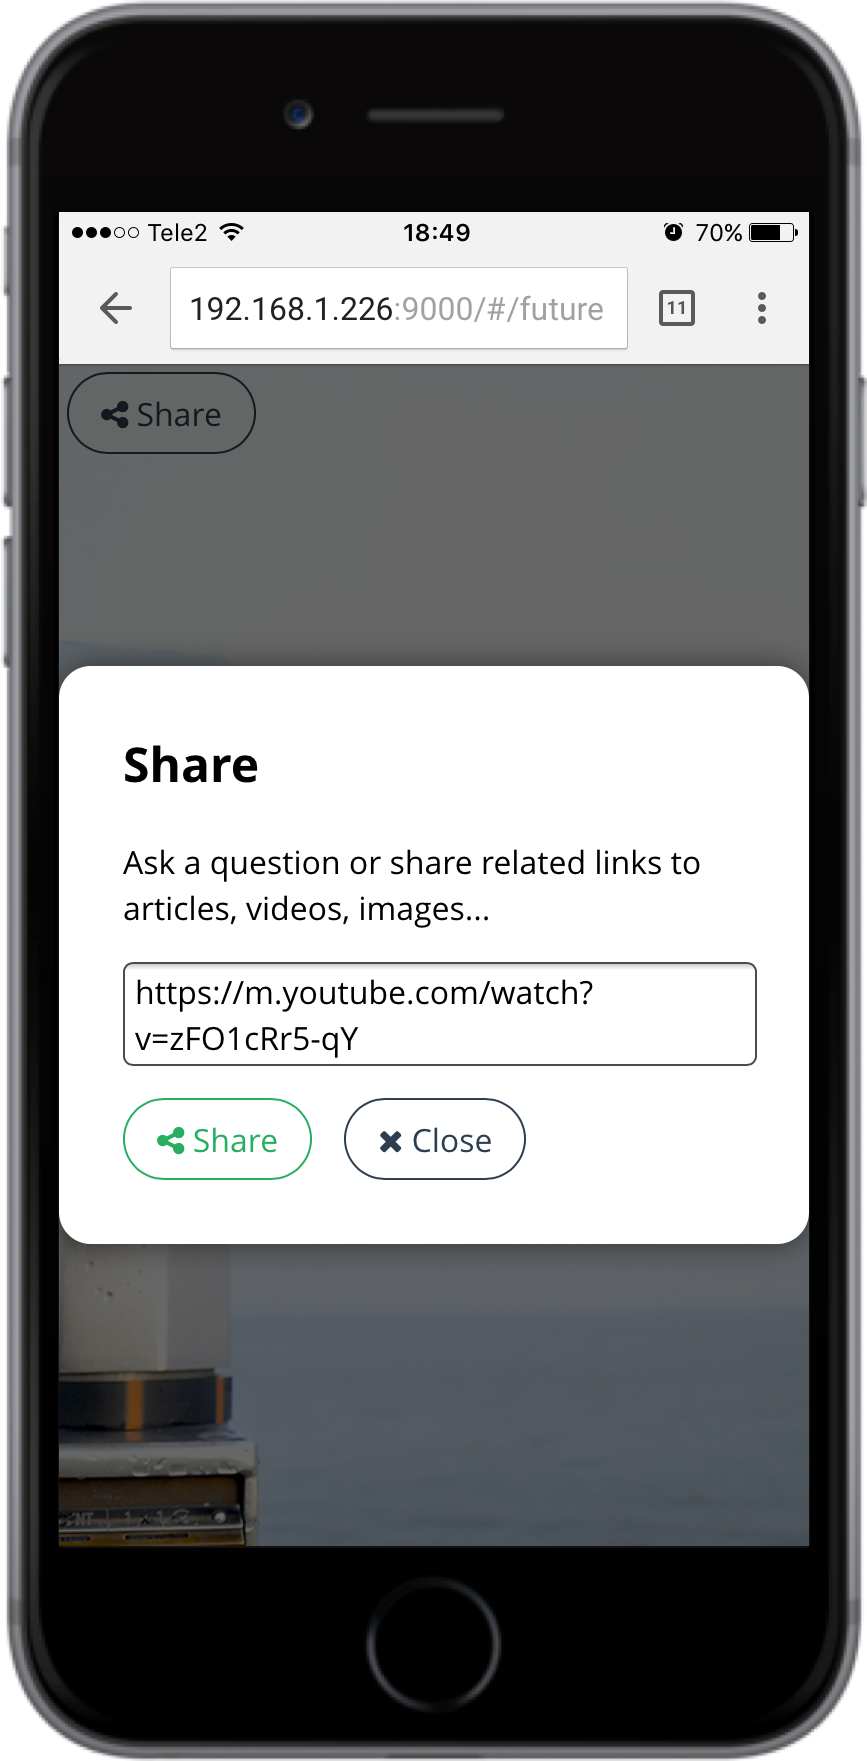
\includegraphics[width=.2\textwidth]{media-screenshot-mobile}
 &
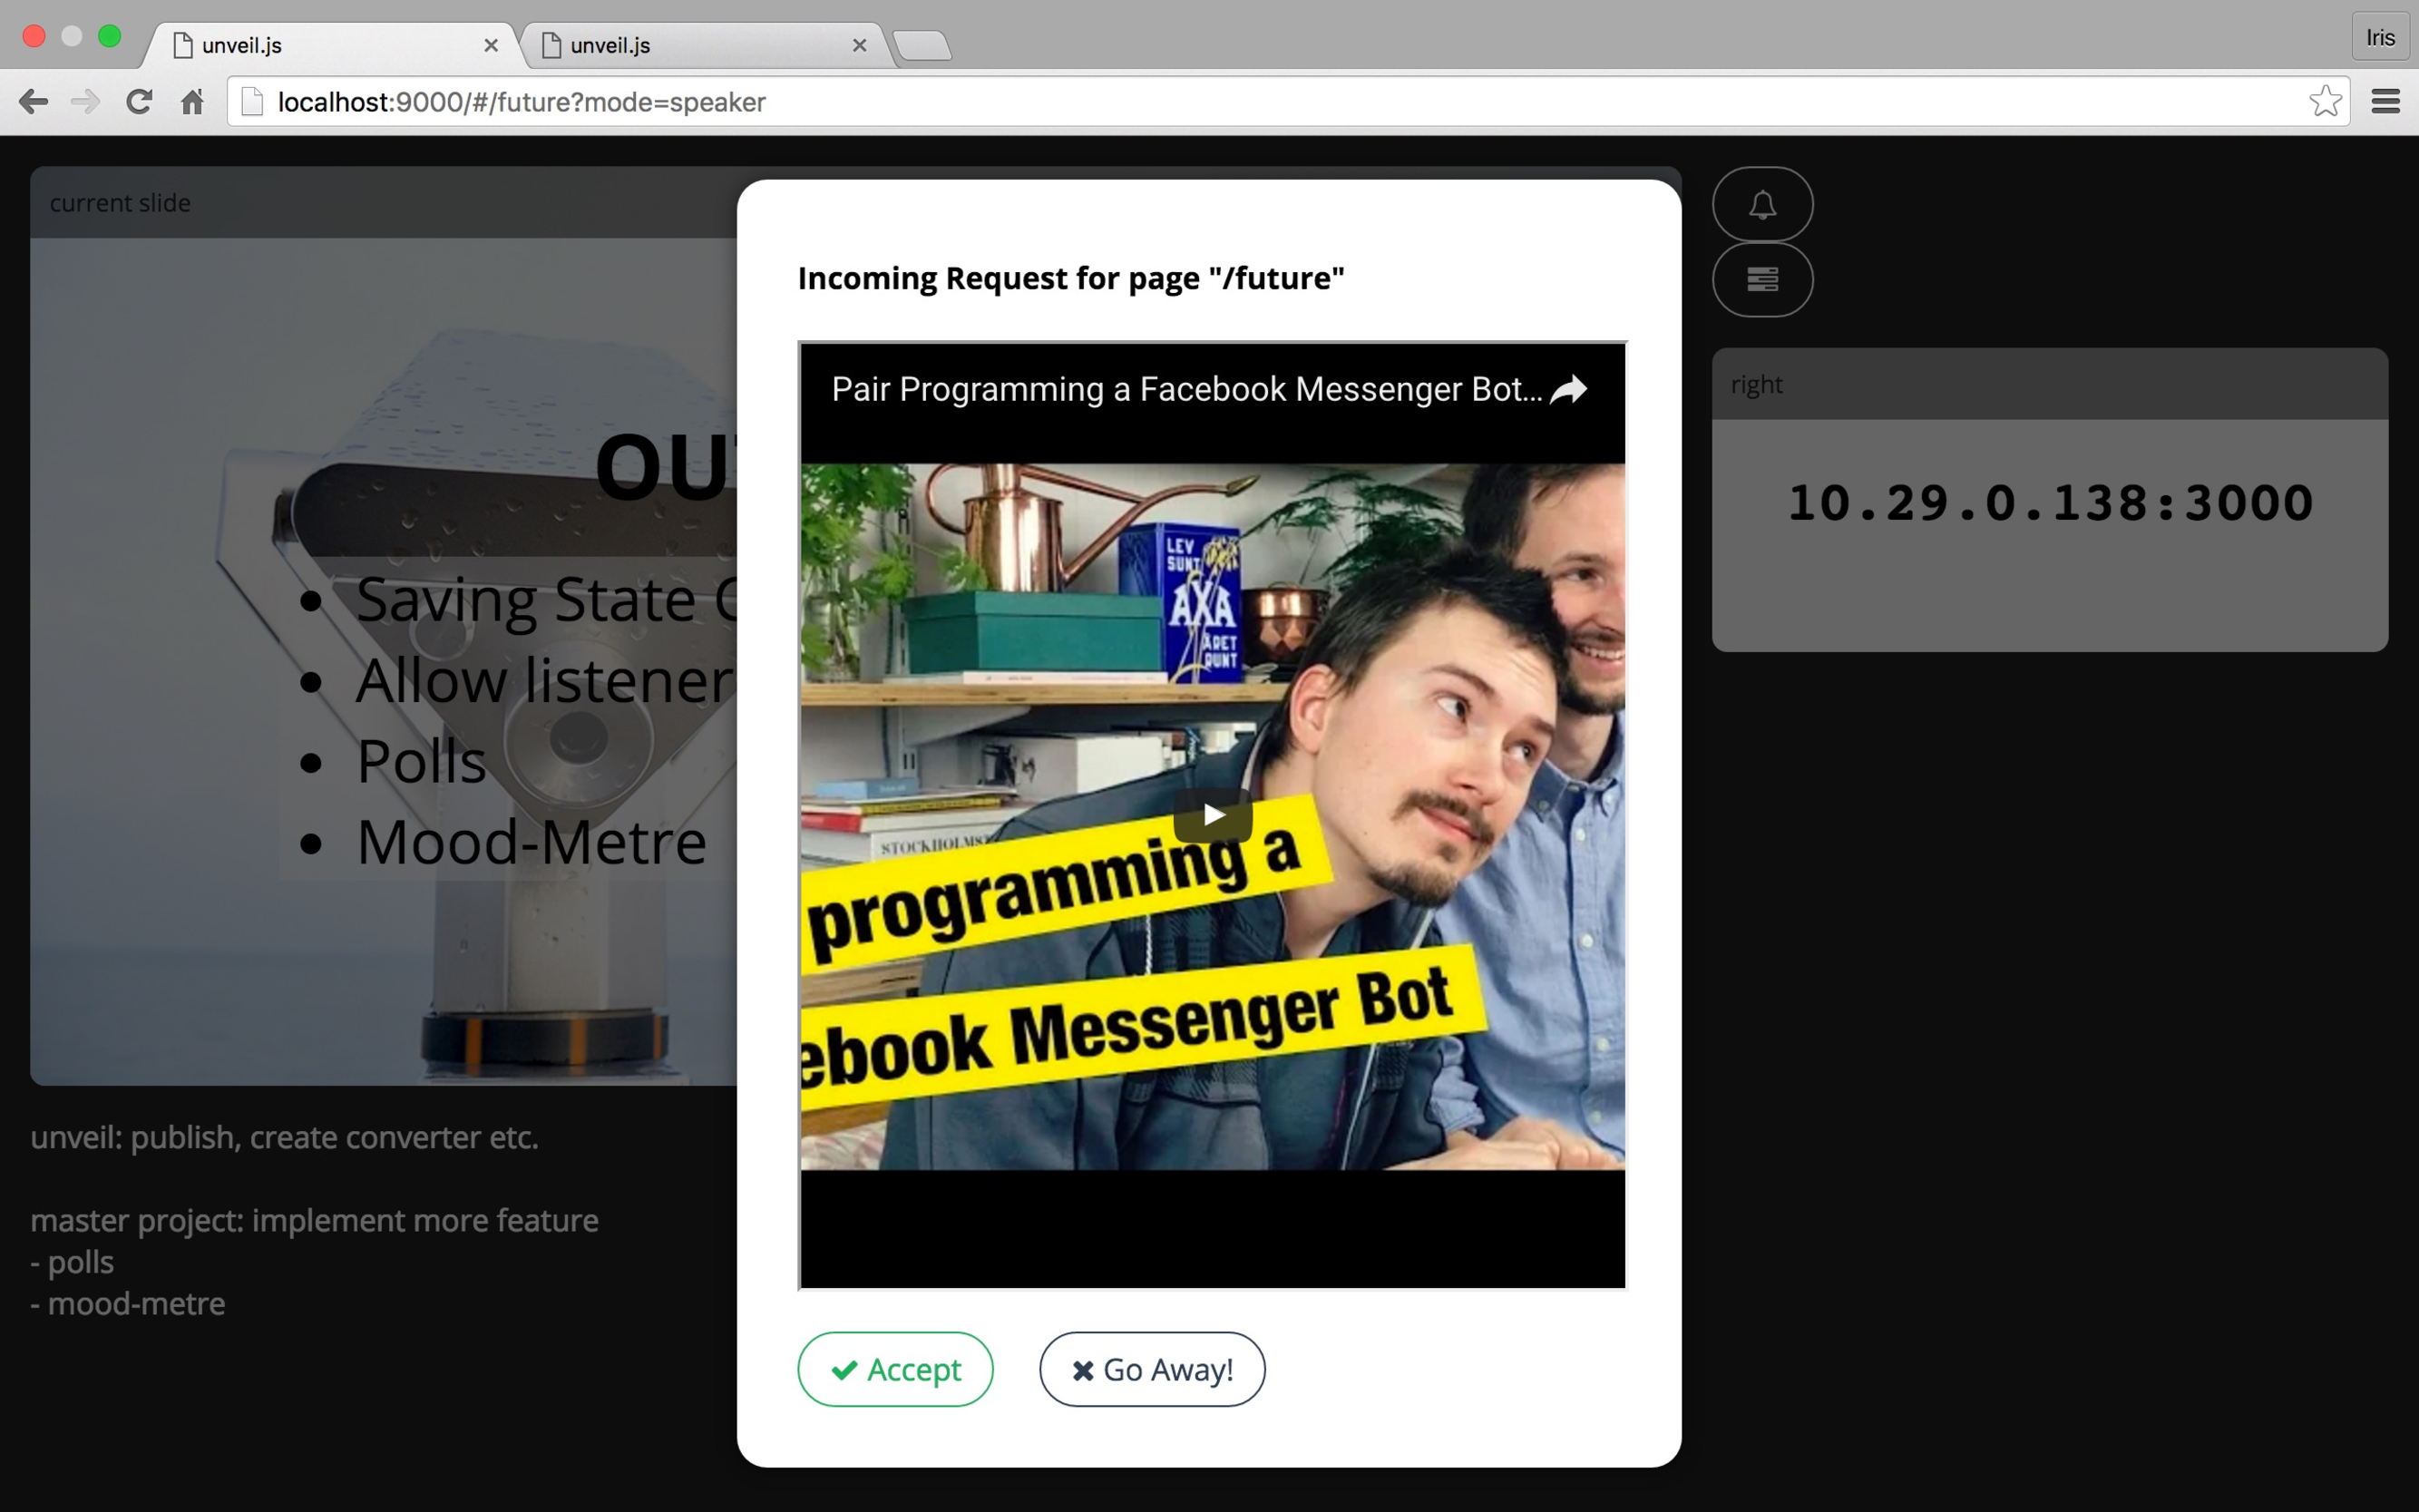
\includegraphics[width=.65\textwidth]{media-acceptor-screenshot} \\
(a) & (b)
\end{tabular}
\caption{Screenshots of sharing content. (a) media sender on mobile phone shares youtube link (b) speaker receives content request.}
\label{fig:implementation-interactive-media}
\end{figure}

\begin{figure}
\centering
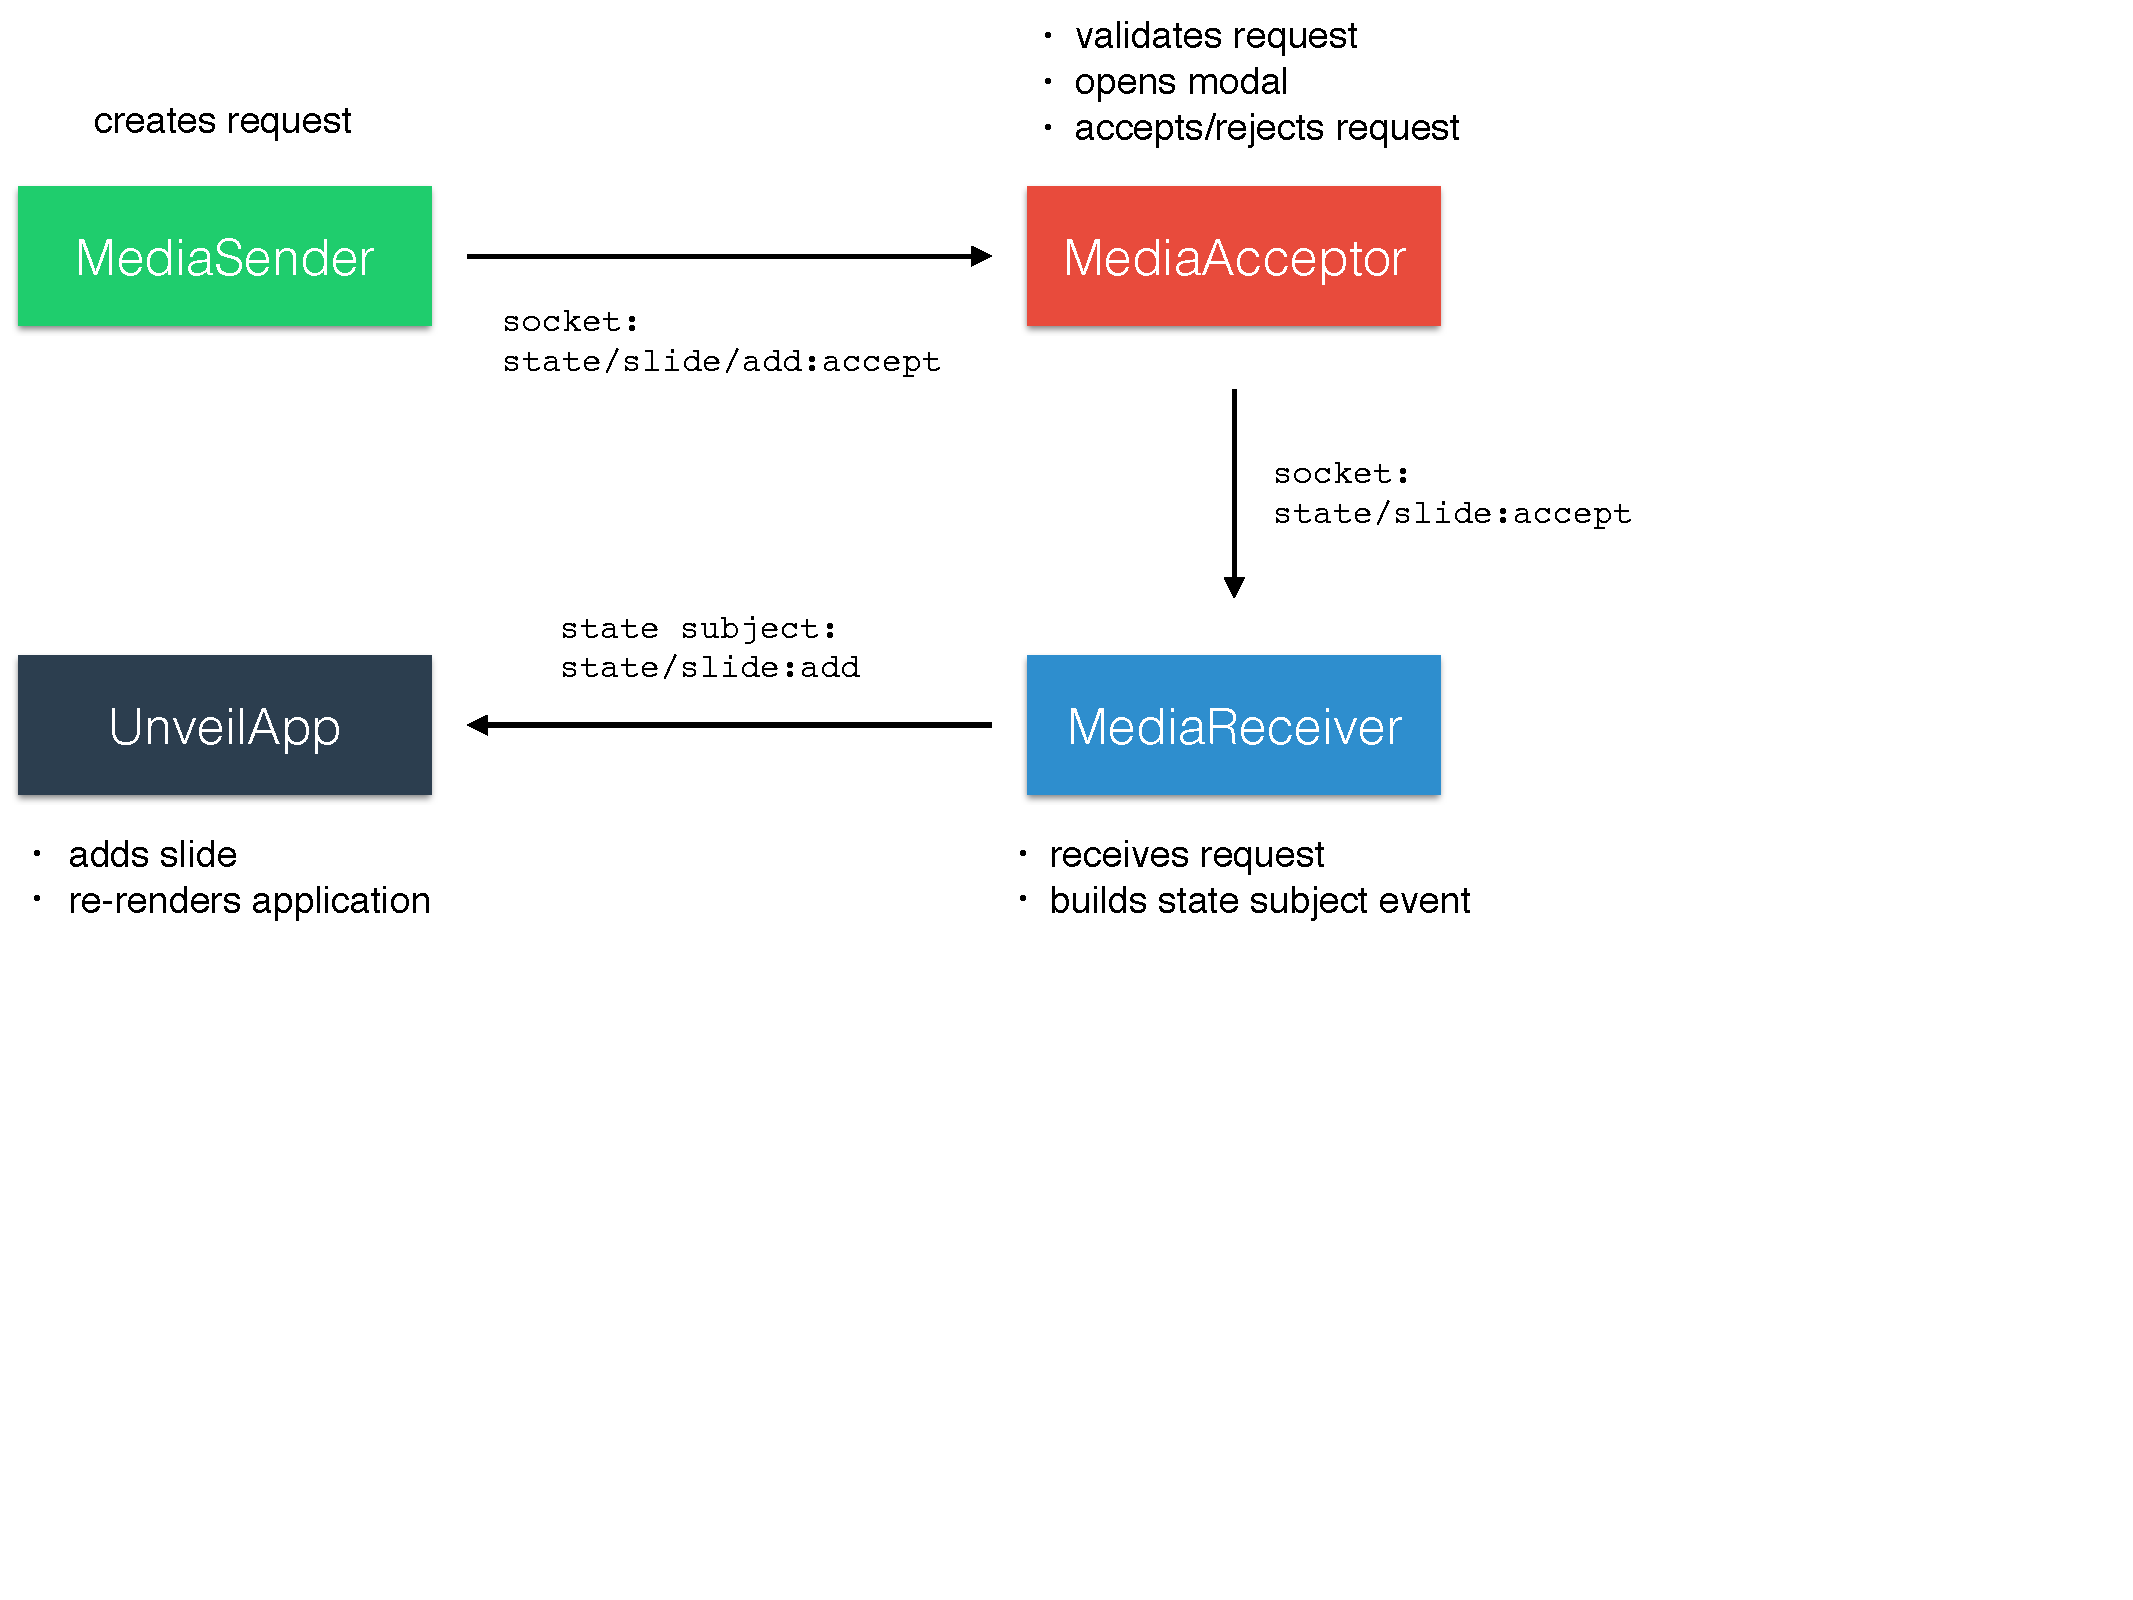
\includegraphics[width=.8\textwidth]{media-pipeline}
\caption{Flow of adding content, monospaced text symbolises type and name of events. First the \texttt{MediaSender} of the default mode sends a request, which the speaker mode's \texttt{MediaAcceptor} listens to. If the request is accepted by the speaker or requests are muted, another socket event is broadcast, which the \texttt{MediaReceiver} waits for. This component is enabled in all modes and emits the state subject event to add a new slide, which \texttt{UnveilApp} reacts to.}
\label{fig:implementation-interactive-media-pipeline}
\end{figure}

\subsection{Voting}
\label{sec:implementation-interactive-voting}

The last group of components connected to the interactive extension covered in this chapter allow speakers to create votings (both during in the preparation of the presentation and on-the-fly as shown in figure \ref{fig:implementation-interactive-voting}) and members of the audience to vote (see figure \ref{fig:implementation-interactive-mobile} (c) and (d)).

\begin{figure}
\centering
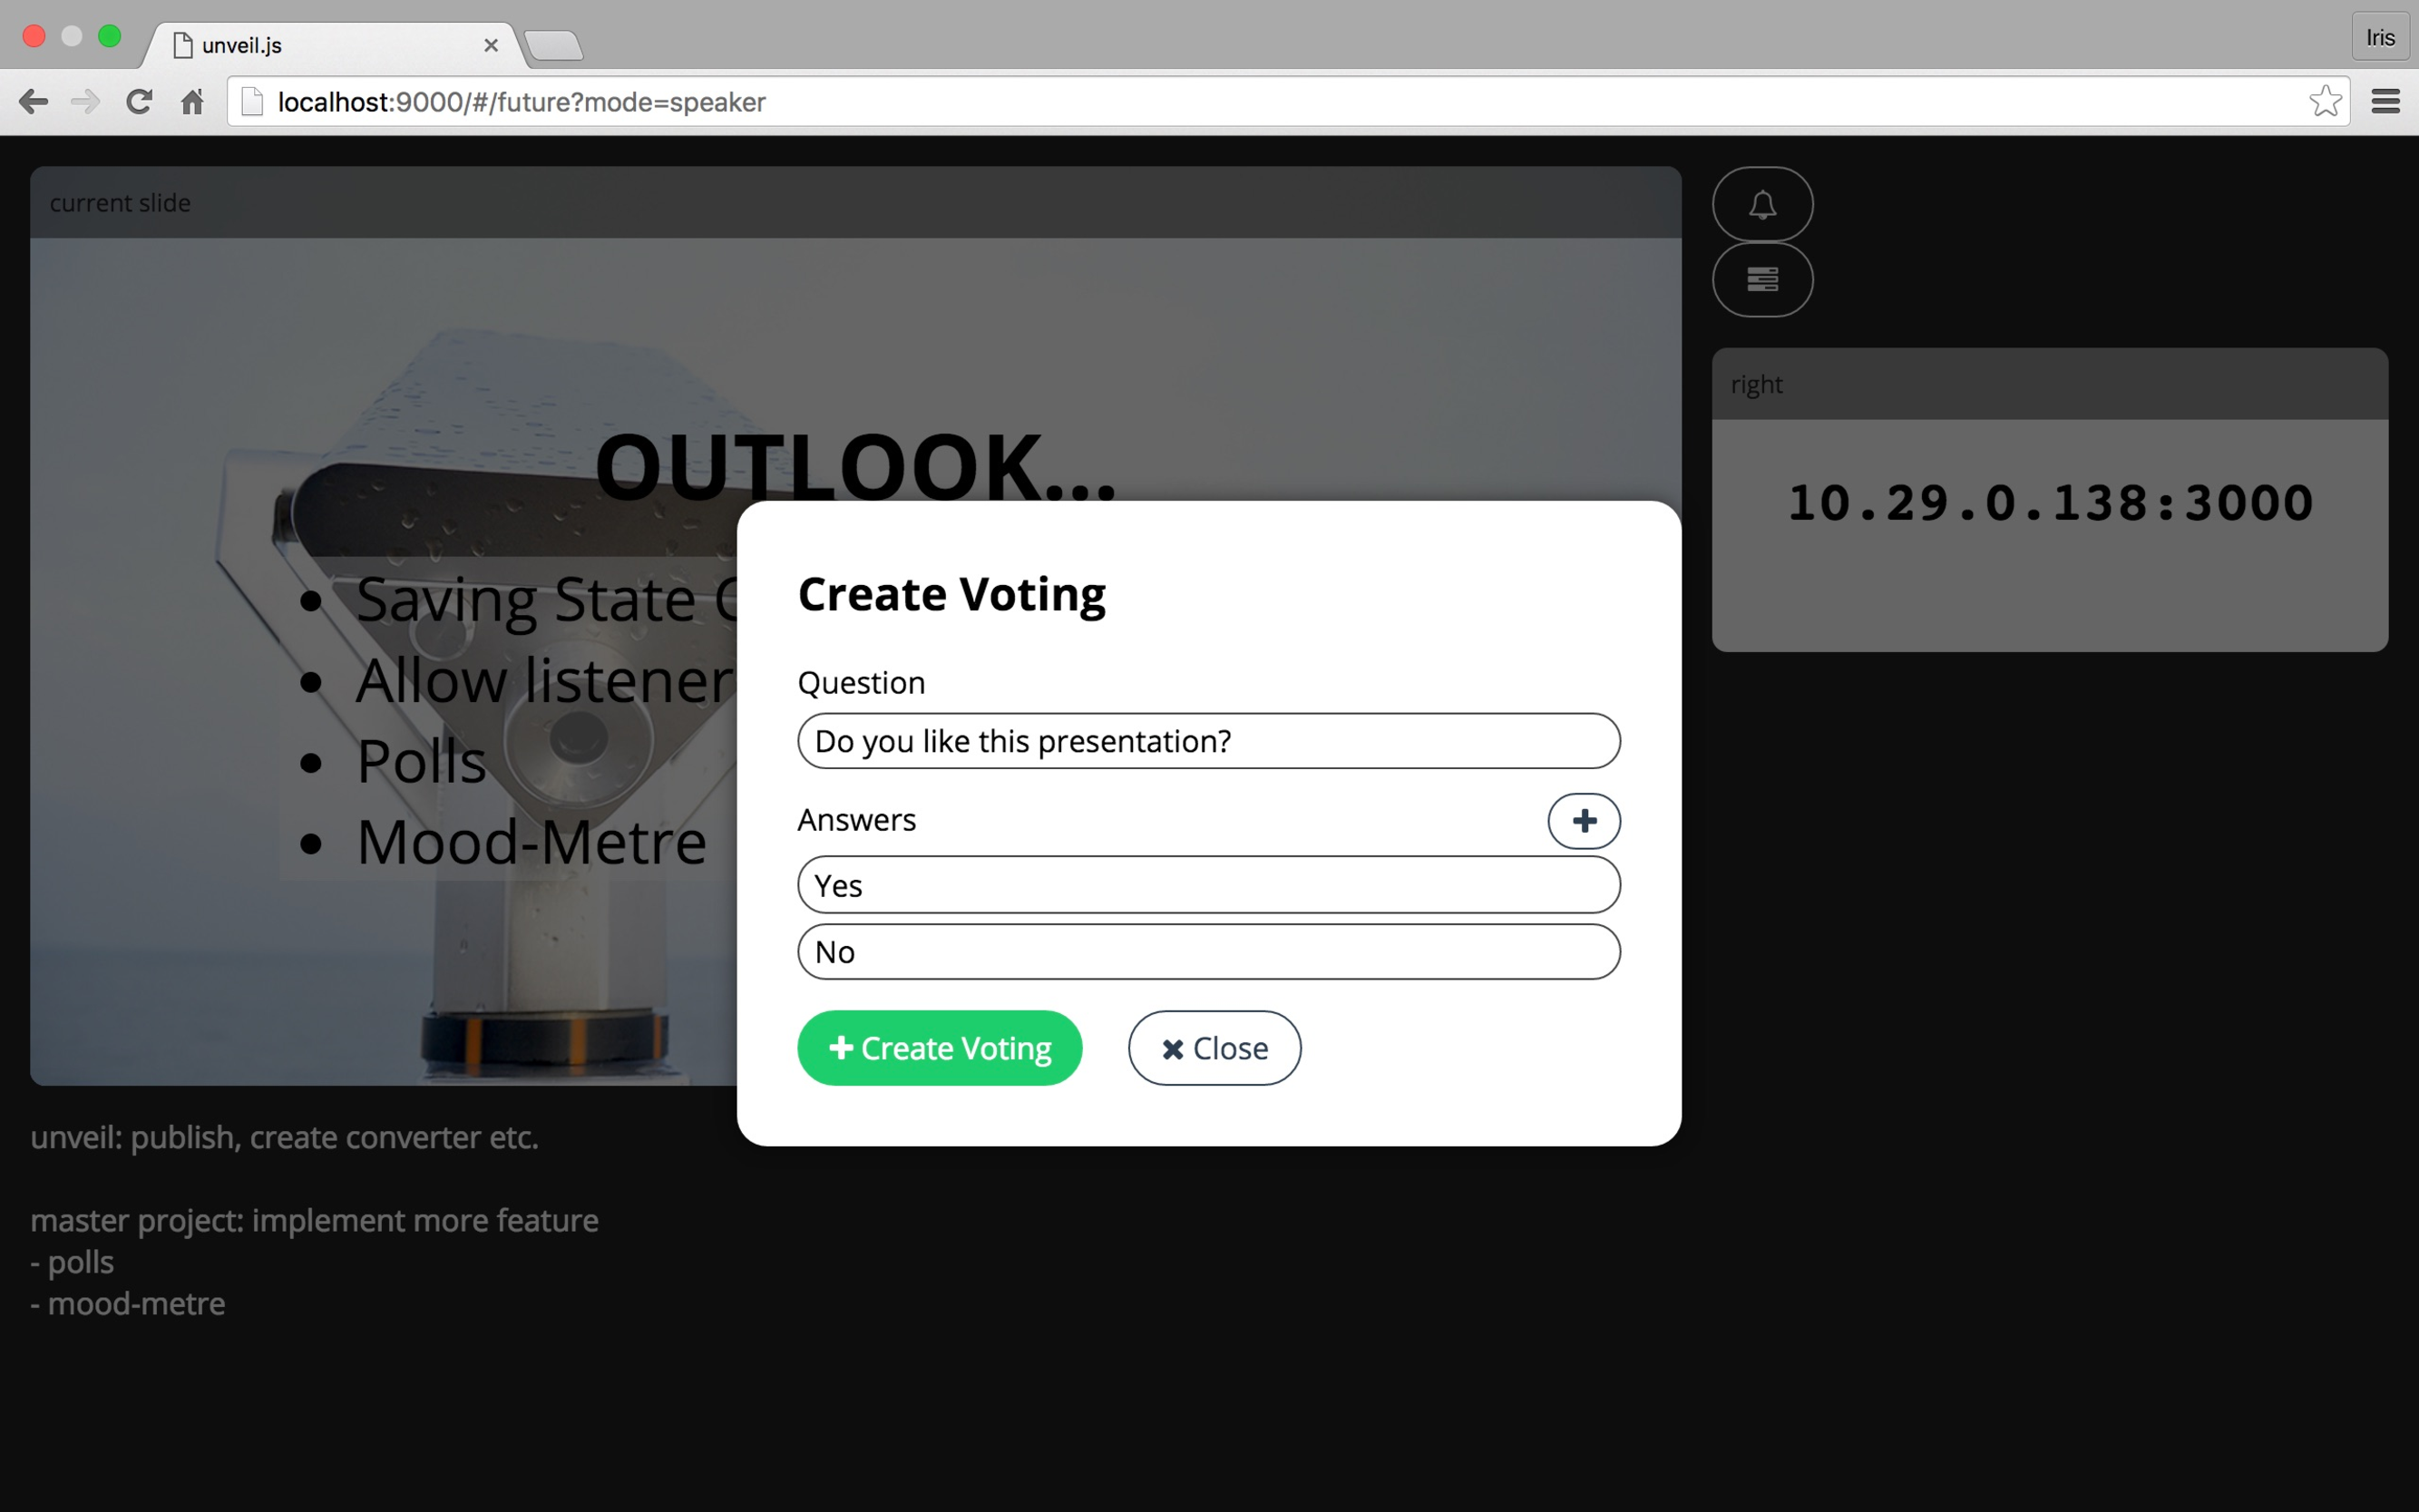
\includegraphics[width=.65\textwidth]{voting-creation-screenshot}
\caption{Screenshot of the desktop speaker mode, creating a new voting, on-the-fly, during a presentation.}
\label{fig:implementation-interactive-voting}
\end{figure}

The main presentational component involved in the voting process is \texttt{Voting}, which keeps track of the current voting scores and has a \texttt{Question} and a number of \texttt{Answer} components as children (see program \ref{prog:implementation-interactive-structure}). \texttt{Voting} also remembers if an audience member has already voted and if so, displays \texttt{Result} components. In speaker and presenter mode only these results are shown.

\begin{program}
\caption{Example code for preparing a slide with voting.}
\label{prog:implementation-interactive-structure}
\begin{JsCode}
<Voting name="like">
  <Question>Do you like these slides?</Question>
  <Answer value="yes">Yes</Answer>
  <Answer value="no">No</Answer>
</Voting>
\end{JsCode}
\end{program}

The audience can start voting as soon as the speaker navigates to the slide with the voting, until then the vote button is disabled. Once the voting has started, the possibility for all audience members to navigate to a different slide is disabled. This happens in the \texttt{VotingNavigatableSetter}, which is only installed for default mode. The voting start event, as well as the voting end event are broadcast by the \texttt{VotingController}, which checks the speaker's current slide for the occurence of a \texttt{Voting}.

Once the voting has started, internally, the \texttt{Voting} component remembers which answer the user has clicked in the \texttt{answer} state variable. Once the submit button is pressed, a \texttt{state/slide/voting:answer} event is fired and broadcast to all clients, which update their internal voting results.
Because the results of the voting should be available throughout the whole presentation and not be reset when leaving the slide, \texttt{Voting} also handles the communication with local storage, to store current results.

\section{Server}
\label{sec:implementation-server}
% shortly talk about server and how any server could really be used for this.
As shortly outlined before, the focus of this project was never the server, but instead the client. For this reason the server was kept as lightweight and dumb as possible, only handling the most important communication. In reality, it acts as a proxy and broadcaster between the clients and serves the JavaScript and HTML files.

The server developed for the project presentation of the Interactive Media course IM690 runs on Node.js, using Express\footnote{\url{http://expressjs.com/}} as a framework. To emphasise how low the requirements for such a server are, a working example implementation can be found in program \ref{prog:implementation-server-code}. Additionally to this code, the server in the unveil-client-server repository also includes a \texttt{lastState} variable, in which the last navigation state is stored. Every time a new client connects, this state is then emitted with a \texttt{state:initial} event. Moreover, socket.io does not currently support wildcards in events, which is why it was necessary to add the code snippet discussed in \cite{socket-io-wildcards}.

\begin{program}
\caption{Very simple possible implementation of a server running the thesis project with Node.js and Express. \cite{socket-io-wildcards} describes how wildcard support can be added to socket.io.}
\label{prog:implementation-server-code}
\begin{JsCode}
var express = require('express');
var app = express();
var server = require('http').createServer(app);
var io = require('socket.io')(server);

// directory 'client' will be served by server
app.use(express.static(__dirname + '/../client/'));

// setting up of socket io
io.on('connection', function(socket) {
  socket.on('*', function(event, data) {
    io.emit(event, data);
  });
});

server.listen(9000, function () {
  console.log('Unveil server listening on port 9000!');
});
\end{JsCode}
\end{program}

\section{Example Application}
\label{sec:implementation-client}
% how is everything defined? what has to be included?
% what are the steps of building an application with unveil?
% how are the slides defined? how are they styled? what about the modes?

To conclude this chapter, I want to show how all the discussed libraries in the end can be put together to a presentation. The whole presentation can be found in the unveil-client-server repository.

The first step to use unveil.js and its extensions is to start a new project, require the necessary npm packages and set up an \texttt{index.html} page which includes the necessary stylesheets and scripts.
The entry point for these scripts is the file \texttt{index.js}, in which the whole presentation is set up and unveil.js is configured by setting up its modes (see program \ref{prog:implementation-client-modes}). As explained before, slides are defined in HTML using the components unveil.js and its extensions provide. An example of this is shown in program \ref{prog:implementation-client-presentation}.

\begin{program}
\caption{Mode definition for setting up an unveil.js presentation. Speaker and projector modes are omitted to keep the example short but follow the same pattern as the default mode.}
\label{prog:implementation-client-modes}
\begin{JsCode}
const modes = {
  default: {
    controls : [
      KeyControls, TouchControls, UIControls,
      NavigationReceiver,
      MediaSender, MediaReceiver,
      VotingNavigatableSetter, VotingReceiver
    ],
    presenter: Presenter
  },
  speaker: {...},
  projector: {...}
};
\end{JsCode}
\end{program}

\begin{program}
\caption{Creation of presentation using modes from program \ref{prog:implementation-client-modes}. Sets up two slides as an example. The DOM will be attached to the element of id \texttt{unveil} in the base HTML document.}
\label{prog:implementation-client-presentation}
\begin{JsCode}
ReactDOM.render((
  <UnveilApp modes={modes}>
    <Slide name="start">
      <h1>Unveil</h1>
      <h2>a meta presentation</h2>
    </Slide>
    <Slide name="problem">
      <img src="./img/problem.png" />
      <Notes>someone always wanted to show something from their device</Notes>
    </Slide>
    ...
  </UnveilApp>
), document.getElementById('unveil'));
\end{JsCode}
\end{program}

The styling of the presentation is handled by CSS. The \texttt{Slide} component automatically adds the name of a slide as its id, allowing to efficiently style slide by slide, as well as applying styles for all slides at once using the \texttt{.slide} class. Program \ref{prog:implementation-client-styles} shows an example of how to style slides.

\begin{program}
\caption{Example styling for slides using Sass. In this particular piece of code, the font family of all slides is set and a background image is added to the start slide.}
\label{prog:implementation-client-styles}
\begin{CssCode}
  .slide
    font-family: 'Open Sans'
  #start
    background-image: url('../img/explore.jpg')
\end{CssCode}
\end{program}
%\chapter{Einleitung}
\label{cha:Einleitung}

\section{Zielsetzung}
Dieses Dokument ist als vorwiegend technische Starthilfe für das
Erstellen einer Masterarbeit (oder Bachelorarbeit) mit \latex
gedacht und ist die Weiterentwicklung einer früheren
Vorlage\footnote{Nicht mehr verfügbar.} für das Arbeiten mit
Microsoft \emph{Word}. Während ursprünglich daran gedacht war, die
bestehende Vorlage einfach in \latex zu übernehmen, wurde rasch
klar, dass allein aufgrund der großen Unterschiede zum Arbeiten
mit \emph{Word} ein gänzlich anderer Ansatz notwendig wurde. Dazu
kamen zahlreiche Erfahrungen mit Diplomarbeiten in den
nachfolgenden Jahren, die zu einigen zusätzlichen Hinweisen Anlass gaben.

Das vorliegende Dokument dient einem zweifachen Zweck: 
\emph{erstens} als Erläuterung und Anleitung, \emph{zweitens} als
direkter Ausgangspunkt für die eigene Arbeit. Angenommen wird,
dass der Leser bereits über elementare Kenntnisse im Umgang mit
\latex verfügt. In diesem Fall sollte -- eine einwandfreie
Installation der Software vorausgesetzt -- der Arbeit nichts mehr
im Wege stehen. Auch sonst ist der Start mit \latex\ nicht
schwierig, da viele hilfreiche Informationen auf den zugehörigen
Webseiten zu finden sind (s.\ Kap.~\ref{cha:ArbeitenMitLatex}).





\section{Warum {\latex}?}

Diplomarbeiten, Dissertationen und Bücher im
technisch-natur\-wissen\-schaft\-lichen Bereich werden
traditionell mithilfe des Textverarbeitungssystems \latex
\cite{Lamport94,Lamport95} gesetzt. Das hat gute Gründe, denn
\latex ist bzgl.\ der Qualität des Druckbilds, des Umgangs mit
mathematischen Elementen, Literaturverzeichnissen etc.\
unübertroffen und ist noch dazu frei verfügbar. Wer mit \latex
bereits vertraut ist, sollte es auch für die Abschlussarbeit
unbedingt in Betracht ziehen, aber auch für den Anfänger sollte
sich die zusätzliche Mühe am Ende durchaus lohnen.

Für den professionellen elektronischen Buchsatz wurde früher
häufig \emph{Adobe Framemaker} verwendet, allerdings ist diese
Software teuer und komplex. Eine modernere Alternative dazu ist
\emph{Adobe InDesign}, wobei allerdings die Erstellung
mathematischer Elemente und die Verwaltung von Literaturverweisen
zur Zeit nur rudimentär unterstützt werden.%
\footnote{Angeblich werden aber für den (sehr sauberen) Schriftsatz 
in \emph{InDesign} ähnliche Algorithmen wie in \latex\ verwendet.}

Microsoft \emph{Word} gilt im Unterschied zu \latex, 
\emph{Framemaker} und \emph{InDesign} übrigens nicht als professionelle
Textverarbeitungssoftware, obwohl es immer häufiger auch von
großen Verlagen verwendet wird.%
\footnote{Siehe auch \url{http://latex.tugraz.at/mythen.php}.}
Das Schriftbild in \emph{Word}
lässt -- zumindest für das geschulte Auge -- einiges zu wünschen
übrig und das Erstellen von Büchern und ähnlich großen Dokumenten
wird nur unzureichend unterstützt. Allerdings ist \emph{Word} sehr
verbreitet, flexibel und vielen Benutzern zumindest oberflächlich
vertraut, sodass das Erlernen eines speziellen Werkzeugs wie
\latex\ ausschließlich für das Erstellen einer Abschlussarbeit
manchen verständlicherweise zu mühevoll ist. Es sollte daher
niemandem übel genommen werden, wenn er/sie sich auch bei der Abschlussarbeit
auf \emph{Word} verlässt. Im Endeffekt lässt sich mit etwas
Sorgfalt (und ein paar Tricks) auch damit ein durchaus akzeptables
Ergebnis erzielen. 
Ansonsten sollten auch für \emph{Word}-Benutzer 
einige Teile dieses Dokuments von Interesse sein, insbesondere die
Abschnitte über Abbildungen und Tabellen
(Kap.~\ref{chap:Abbildungen}) und mathematische Elemente
(Kap.~\ref{chap:Mathematik}).

Übrigens, genau hier am Ende des Einleitungskapitels (und nicht
etwa in der Kurzfassung) ist der richtige Platz, um die
inhaltliche Gliederung der nachfolgenden Arbeit zu beschreiben.
Hier soll dargestellt werden, welche Teile (Kapitel) der Arbeit
welche Funktion haben und wie sie inhaltlich zusammenhängen. Auch
die Inhalte des \emph{Anhangs} -- sofern vorgesehen -- sollten hier
kurz beschrieben werden.


%
%\chapter{Die Abschlussarbeit}
\label{cha:Diplomschrift}

Jede Abschlussarbeit%
\footnote{Die meisten der folgenden Bemerkungen gelten gleichsam für Bachelor-, Master- und Diplomarbeiten.} 
ist anders und dennoch sind sich gute
Arbeiten in ihrer Struktur meist sehr ähnlich, \va\ bei
technisch-natur\-wissen\-schaft\-lichen Themen. 

\section{Elemente der Abschlussarbeit}

Als Ausgangspunkt bewährt hat sich der folgende Grundaufbau, der natürlich 
vari\-iert und beliebig verfeinert werden kann:
%
\begin{enumerate}
\item \textbf{Einführung und Motivation}: Was ist die Problem- oder Aufgabenstellung und
warum sollte sich jemand dafür interessieren?
\item \textbf{Präzisierung des Themas}: Hier wird der aktuelle Stand der Technik
oder Wissenschaft ("`State-Of-The-Art"') beschrieben, es werden bestehende
Defizite oder offene Fragen aufgezeigt und daraus die
Stoßrichtung der eigenen Arbeit entwickelt.
\item \textbf{Eigener Ansatz}: Das ist natürlich der Kern der Arbeit. Hier
wird gezeigt, wie die vorher beschriebene Aufgabenstellung gelöst und --
häufig in Form eines Programms%
\footnote{\emph{Prototyp} ist in diesem Zusammenhang ein gerne benutzter Begriff, der im Deutschen
allerdings oft unrichtig dekliniert wird. Richtig ist: der \emph{Prototyp}, des \emph{Prototyps}, dem/den \emph{Protototyp} -- falsch hingegen \zB: des \emph{Prototyp\underline{en}}!
} --
realisiert wird, ergänzt durch illustrative Beispiele.
\item \textbf{Zusammenfassung}: Was wurde erreicht und welche Ziele sind
noch offen geblieben, wo könnte weiter gearbeitet werden?
\end{enumerate}
%
Natürlich ist auch ein gewisser dramaturgischer Aufbau der Arbeit
wichtig, wobei zu bedenken ist, dass der Leser in der Regel nur
wenig Zeit hat und -- anders als etwa bei einem Roman -- seine
Geduld nicht auf die lange Folter gespannt werden darf. Erklären
Sie bereits in der Einführung (und nicht erst im letzten Kapitel),
wie Sie an die Sache herangehen, welche Lösungen Sie vorschlagen
und wie erfolgreich Sie damit waren.

Übrigens, auch Fehler und Sackgassen dürfen (und sollten)
beschrieben werden; ihre Kenntnis hilft oft doppelte Experimente und
weitere Fehler zu vermeiden und ist damit sicher nützlicher als
jede Schönfärberei.
Und natürlich ist es auch nicht verboten, seine eigene Meinung 
in sachlicher Form zu äußern.


\section{Arbeiten in Englisch}
\label{sec:englisch}

Diese Vorlage ist zunächst darauf abgestellt, dass die
Abschlussarbeit in deutscher Sprache erstellt wird. Vor allem bei
Arbeiten, die in Zusammenarbeit mit größeren Firmen oder
internationalen Instituten entstehen, ist es häufig erwünscht,
dass die Abschlussarbeit zu besseren Nutzbarkeit in englischer
Sprache verfasst wird, und viele Hochschulen%
\footnote{Die FH Oberösterreich macht hier keine Ausnahme. 
Der Begriff "`Fachhochschule"' wird dabei entweder gar nicht
übersetzt oder -- wie im deutschsprachigen Raum mittlerweile üblich -- 
mit \emph{University of Applied Sciences}.
%Die offizielle englische Übersetzung von "`Medientechnik und -design"'
%ist übrigens \emph{Media Technology and Design}.
} 
lassen dies in
der Regel auch zu.

Beachtet sollte allerdings werden, dass das Schreiben dadurch nicht
einfacher wird, auch wenn einem Worte und Sätze im Englischen
scheinbar leichter "`aus der Feder"' fließen. Gerade im Bereich
der Informatik erscheint durch die Dominanz englischer
Fachausdrücke das Schreiben im Deutschen mühsam und das Ausweichen
ins Englische daher besonders attraktiv. Das ist jedoch
trügerisch, da die eigene Fertigkeit in der Fremdsprache
(trotz der meist langjährigen Schulbildung) häufig überschätzt wird.
Prägnanz und Klarheit gehen leicht verloren und bisweilen ist das
Resultat ein peinliches Gefasel ohne Zusammenhang und soliden
Inhalt. Sofern die eigenen Englischkenntnisse nicht wirklich gut sind, ist
es ratsam, zumindest die wichtigsten Teile der Arbeit zunächst in
Deutsch zu verfassen und erst nachträglich zu übersetzen. Besondere Vorsicht ist bei der Übersetzung von scheinbar
vertrauten Fachausdrücken angebracht. Zusätzlich ist es immer zu
empfehlen, die fertige Arbeit von einem "`native speaker"'
korrigieren zu lassen.



Technisch ist, außer der Spracheinstellung und den
unterschiedlichen Anführungszeichen (s.\
Abschn.~\ref{sec:anfuehrungszeichen}), für eine englische Arbeit
nicht viel zu ändern, allerdings sollte Folgendes beachtet werden:
%
\begin{itemize}
\item  Die Titelseite (mit der Bezeichnung "`Diplomarbeit"' oder "`Masterarbeit"') 
ist für die einzureichenden Exemplare jedenfalls in \emph{deutsch} zu halten,
auch wenn der Titel englisch ist. 
\item Ebenso muss neben dem
englischen \emph{Abstract} auch eine deutsche \emph{Kurzfassung}
enthalten sein. %
\item Akademische Titel von Personen haben im Englischen offenbar
weniger Bedeutung als im Deutschen und werden daher meist
weggelassen.
\end{itemize}

%
%\chapter{Zum Arbeiten mit \latex}
\label{cha:ArbeitenMitLatex}

\section{Einstieg}
\label{sec:LatexEinstieg}

\latex ist eine in den Naturwissenschaften sehr verbreitete
und mittlerweile klassische Textverarbeitungssoftware für das Erstellen
großer und komplizierter Dokumente mit professionellem Anspruch.
Das Arbeiten mit \latex erscheint -- zumindest für den ungeübten Benutzer -- %
zunächst schwieriger als mit herkömmlichen Werkzeugen für die
Textverarbeitung.

Zum Ersten ist -- im Unterschied zu den meisten gängigen
Text\-ver\-arbei\-tungs\-prog\-ram\-men -- \latex nicht \textsc{Wysiwyg}%
\footnote{"`What You See Is What You Get."' Es gibt auch 
\textsc{Wysiwyg}-Implementierungen für \latex, 
\zB\ \emph{Scientific WorkPlace} (\url{http://www.mackichan.com/}) oder
\emph{LyX} (\url{http://www.lyx.org/}), 
die aber teuer \bzw\ relativ langsam sind.},
sondern es handelt sich um eine \emph{Markup Lang\-uage} (wie HTML) -- noch dazu
eine für den Anfänger recht komplizierte -- und zugehörige Werkzeuge.
Ungewohnt erscheinen sicher auch die vermeintlich starken
Einschränkungen von \latex,
insbesondere in Bezug auf die Wahl der Schriften und das
Layout. Während anfangs of der Eindruck entsteht, dass diese Rigidität
die eigene Kreativität beschränkt, fällt mit der Zeit auf, dass es gerade
dadurch gelingt, sich stärker auf die Inhalte der Arbeit zu
konzentrieren als auf deren äußere Form. Dass am Ende die Form dennoch stimmt,
ist allerdings nur dann gewährleistet, wenn man sich bei den eigenen Modifikationen
der Formate und Parameter äußerste Zurückhaltung auferlegt, es sei denn,
man ist in der Zwischenzeit bereits selbst zum \latex-\emph{Guru} avanciert.

Insgesamt lohnt sich der Aufwand, wie viele meinen, zumal die Abschlussarbeit
in jedem Fall (mit oder ohne \latex) ein substantielles Stück Arbeit ist.
Allerdings sollte mithilfe von \latex ein professionell aussehendes
Ergebnis einfacher zu erreichen sein und es dürfte wohl auch einiger
Ärger mit Fehlern und Einschränkungen gängiger Software erspart bleiben.
Zudem könnte es durchaus sein, dass sich nebenbei auch das eigene Auge für
die Feinheiten des Buchsatzes (weiter-){\obnh}entwickelt.%
\footnote{Dieses abschließende Textelement wurde übrigens zur Ermöglichung eines 
Zeilenumbruchs nach der Klammer so gesetzt: \texttt{\ldots (weiter-)\{{\bs}optbreaknh\}entwickelt.}
Das Makro \texttt{{\bs}optbreaknh} ("`optional break with no hyphen"') ist in 
\texttt{hgb.sty} definiert.}


\subsection{Software}
\label{sec:Software}

Zum Arbeiten mit \latex wird -- neben einem Computer -- natürlich Software benötigt. Mussten früher oft die einzelnen Komponenten von \latex mühevoll zusammengesucht und für die eigene Umgebung konfiguriert werden, gibt es mittlerweile für die wichtigsten Plattformen (Windows, Mac~Os, Linux) fertige \latex-Installationen, die ohne weiteres Zutun laufen. Die aktuelle Version von \latex\ ist \LaTeXe\ (sprich "`LaTeX zwei e"'). 
Zum Arbeiten mit \latex\ werden zwei Dinge benötigt:
%
\begin{itemize}
\item \latex-Installation (Distribution),
\item Texteditor oder Autorenumgebung (Frontend).
%\item PostScript/PDF-Software 
\end{itemize}
%
Sämtliche Komponenten sind kostenlos und für alle gängigen Plattformen verfügbar.


\subsubsection{Windows}
\label{sec:Windows}

Unter \emph{Windows} (XP und höher) hat sich folgendes Setup bewährt,
mit dem \ua auch dieses Dokument erstellt wurde:
%
\begin{itemize}
\item \textbf{\latex-Distribution}: \emph{MikTeX 2.9}\footnote{\url{http://www.miktex.org/}} oder höher.
MikTeX enthält bereits alle notwendigen Hilfsprogramme, wie beispielsweise {\tt pdflatex}.

\item \textbf{PDF-Viewer}: \emph{SumatraPDF}.%
\footnote{\url{http://blog.kowalczyk.info/software/sumatrapdf/}}

\item \textbf{Frontend}: \emph{TeXnicCenter}.%
\footnote{\url{www.texniccenter.org}}
Grundsätzlich kann jeder Texteditor%
\footnote{Unter Windows \zB\ \emph{Notepad++} (\url{http://notepad-plus-plus.org/}).}
verwendet werden, praktischer ist jedoch eine integrierte \latex-Um\-geb\-ung wie TeXnicCenter, die einen auch bei 
der Dateiverwaltung, der Verarbeitung der Dokumente und der Fehlerbehandlung unterstützt.
Eine interessante Alternative bietet die Verwendung von \emph{Eclipse}\footnote{\url{http://www.eclipse.org/}}
als plattformunabhängiges Frontend 
(mit dem \emph{TeXlipse}\footnote{\url{http://texlipse.sourceforge.net/}} Plugin).
\end{itemize}
%
Beim erstem Mal sollten \emph{MikTeX}, \emph{SumatraPDF} und \emph{TeXnicCenter} in genau dieser Reihenfolge installiert werden.

Als Gesamtpaket bietet sich \emph{TeXstudio}\footnote{\url{http://texstudio.sourceforge.net/}} an. 
In diesem Fall kann die Installation eines separaten PDF-Viewers entfallen, denn dieser ist in der 
Software bereits enthalten.

\subsubsection{Mac~OS}
\label{sec:MacOs}

Unter Mac~OS~X ist die Referenzdistribution \emph{MacTeX}.%
\footnote{\url{http://www.tug.org/mactex}} 
Sie enthält neben der TeX-Distribution \emph{TeX Live} auch gängige Editoren wie \emph{TeXWorks} oder \emph{TeXshop}. Mit dem \emph{TeX Live Utility} können Pakete verwaltet und die Distribution auf den neuesten Stand gebracht werden. Als Alternative zu den beiden genannten Editoren steht \emph{TeXnicle}%
\footnote{\url{http://www.bobsoft-mac.de/texnicle/texnicle.html}} zur Verfügung. Er bietet -- ähnlich wie \emph{TeXnicCenter} unter Windows -- einen projektbasierten Workflow an.
Ebenso ist auch \emph{TeXstudio} für Mac~OS~X 10.8 und neuer verfügbar.
Ein PDF-Viewer muss unter Mac~OS~X übrigens nicht extra installiert werden. Alle genannten Editoren beinhalten eine eigene PDF-Vorschau.

%ALT:
%Bewährte und weit verbreitete Frontends für den Mac sind \emph{MacTeX}%
%\footnote{\url{www.tug.org/mactex} -- enthält eine komplette und fertig konfigurierte LaTeX-Installation 
%für Mac~OS (ca.\ 1.15 GB download).}
%und \emph{TeXShop},%
%\footnote{\url{www.uoregon.edu/~koch/texshop/}}
%das üblicherweise zusammen mit der TeX-Distribution \emph{TeX Live} verwendet wird. 
%Weit verbreitet ist auch der \emph{TeXworks} Editor, der ebenfalls im MacTeX Package enthalten ist und auch MiKTeX unter Windows beigefügt ist.


\subsubsection{Linux}

Auch unter Linux ist \emph{TeX Live} (\so) eine häufig verwendete TeX-Distri\-bution. 
Als Frontend sind beispielsweise
\emph{Lyx}\footnote{\url{http://www.lyx.org/}},
\emph{Kile}\footnote{\url{http://kile.sourceforge.net/}} und
\emph{Texmaker}\footnote{\url{http://www.xm1math.net/texmaker/}} 
verbreitet.
\emph{TeXstudio} ist ebenfalls für alle gängigen Distributionen über die jeweiligen Paket-Manager erhältlich. Alternativ können die entsprechenden Packages von der Webseite bezogen werden.
In manchen gängigen Linux-Versionen ist bereits eine komplette \latex-Distribution enthalten, sodass im besten Fall überhaupt keine zusätzliche Installation notwendig ist.  


\subsection{Literatur}
\label{sec:literatur}

Es ist müßig, ohne geeignete Literatur mit \latex zu beginnen, selbst
fortgeschrittene Benutzer werden immer wieder auf Hilfe angewiesen
sein. Erfreulicherweise ist sehr viel Nützliches auch online verfügbar.
Gute Startpunkte sind \zB
%
\begin{itemize}
\item \emph{{\rm\LaTeXe}-Kurzbeschreibung} von Daniel et al.\ \cite{Daniel2012}
\item \emph{The Not So Short Introduction to {\rm \LaTeXe}}
            von Oetiker et al.\ \cite{Oetiker2014}
\end{itemize}
%
\noindent
Als mittlerweile bereits klassisches Handbuch zu \latex ist
%
\begin{itemize}
  \item \emph{A Guide to {\rm\LaTeX}} von H.~Kopka und P.~Daly \cite{Kopka2003}
\end{itemize}
%
zu empfehlen, zu dem es für Interessierte auch zwei vertiefende
Zusatzbände in Deutsch gibt. Zahlreiche weitere Dokumente zu
\latex und verwandten Themen finden sich \ua im Rahmen des {\em
Comprehensive TeX Archive Network} (CTAN) auf
\begin{quote}
	\url{http://www.ctan.org/}%
	\footnote{\url{http://www.ctan.org/topic/}}
\end{quote}
%
Besonders nützlich sind auch die
\emph{Comprehensive List of {\rm \latex} Symbols} \cite{Pakin2009}
und die Beschreibungen wichtiger \latex-Pakete, wie
%
\begin{quote}
	\texttt{babel} \cite{Bezos2014},\newline
% \texttt{german}, \texttt{ngerman} \cite{Raichle98},\newline
  \texttt{grahics}, \texttt{graphicx} \cite{Carlisle2014},\newline
  \texttt{fancyhdr} \cite{Oostrum2004},\newline
  \texttt{caption} \cite{Sommerfeldt2011},\newline
  \texttt{subfig} \cite{Cochran05}.
\end{quote}





\section{Schrift}

In einem \latex-Dokument muss zunächst die verwendete Schriftart festgelegt werden. Im Text können dann mittels diverser Auszeichnungen Textstellen durch eine Änderung des Schriftstils hervorgehoben werden.

\subsection{Schriftarten}

\latex verwendet normalerweise die Schriften der \emph{Computer
Modern}
(CM) Serie, die so wie die \emph{TeX}-Software selbst von Donald Knuth%
\footnote{\url{http://www-cs-faculty.stanford.edu/~uno/}} entwickelt
wurden. Die drei Basis-Schrifttypen der CM-Serie in \latex sind
%
\begin{quote}
\begin{tabular}{lcl}
\textrm{Roman}      & & \verb!\textrm{Roman}!,\\
\textsf{Sans Serif} & & \verb!\textsf{Sans Serif}!,\\
\texttt{Typewriter} & & \verb!\texttt{Typewriter}!.\\
\end{tabular}
\end{quote}
%
\noindent In den Augen vieler Benutzer ist allein die Qualität und
Zeitlosigkeit dieser Schriften ein Grund, \latex für seriöse
Zwecke zu verwenden. Ein weiterer Vorteil der \emph{TeX}-Schriften
ist, dass die unterschiedlichen Schriftfamilien und Schnitte
bezüglich der Größe sehr gut aufeinander abgestimmt sind.

Darüber hinaus können aber in \latex auch beliebige 
\emph{PostScript}-Schrif\-ten (Type 1) verwendet werden, was allerdings in
der Praxis einiges an "`Tuning"'-Arbeit verlangt. Häufig verwendet
werden \zB\ \emph{Times} und \emph{Palatino}, derzeit ist aber ein Trend 
zurück zu den klassischen CM-Schriften zu beobachten.



\subsection{Texte hervorheben}

Texte können auf unterschiedliche Weise aus dem Fließtext hervorgehoben werden.
\begin{itemize}
%
\item Die Auszeichnung in \textit{Kursivschrift} oder "`italic"' (\verb!\textit{..}!) ist \va\ zum Hervorheben von
Betonungen und Zitaten geeignet, aber auch für
Produktbezeichnungen, Fremdwörter und Variablen im Text, \zB
%
\begin{quote}
\verb!\textit{Variable}! $\rightarrow$ \textit{Variable}
\end{quote}
%
\item {\sl Slanted} %
(\verb!\textsl{..}!) bedeutet eine geneigte Schrift und
unterscheidet sich damit deutlich von \textit{Italic}; 
zum Vergleich:
%
\begin{quote}
\verb!\textrm{Daimler-Chrysler}! $\rightarrow$ \textrm{Daimler-Chrysler} \newline%
\verb!\textsl{Daimler-Chrysler}! $\rightarrow$ \textsl{Daimler-Chrysler} \newline%
\verb!\textit{Daimler-Chrysler}! $\rightarrow$ \textit{Daimler-Chrysler}
\end{quote}
%
\item \textbf{Boldface} (\verb!\textbf{..}!) wird \ia\ verwendet für 
\textbf{Überschriften}, Bezeichnungen von \textbf{Abbildungen} und 
\textbf{Tabellen}, im Fließtext aber selten:
%
\begin{quote}
\verb!\textbf{Überschriften}! $\rightarrow$ \textbf{Überschriften}
\end{quote}
%
\item \emph{Emphasize} (\verb!\emph!) %
ist normalerweise gleichbedeutend mit \verb!\textit!, wobei
\verb!\emph{..}! allerdings auch bei geschachtelten
Hervorhebungen und im Bereich anderer Schriftschnitte das
"`Richtige"' tut: 
%
\begin{quote}
\setlength{\tabcolsep}{0pt}%
\begin{tabular}{lcl}
\verb!\textrm{Du \emph{auch} hier?}! & $\;\rightarrow\;$ &
    \textrm{Du \emph{auch} hier?}
\\
\verb!\textit{Du \emph{auch} hier?}! & $\;\rightarrow\;$ &
    \textit{Du \emph{auch} hier?} 
\\
\verb!\textsl{Du \emph{auch} hier?}! & $\;\rightarrow\;$ & 
    \textsl{Du \emph{auch} hier?}
\\
\verb!\textbf{Du \emph{auch} hier?}! & $\;\rightarrow\;$ & 
    \textbf{Du \emph{auch} hier?}
\\
\verb!\texttt{Du \emph{auch} hier?}! & $\;\rightarrow\;$ & 
    \texttt{Du \emph{auch} hier?}
\end{tabular}
\end{quote}
%
\item \underline{Unterstreichungen} sind ein Relikt aus der 
Schreibmaschinenära und im modernen Schriftsatz
eigentlich \underline{überflüssig}. Sie sollten daher nur in
Ausnahmefällen verwendet werden, \zB
%
\begin{quote}
\verb!\underline{überflüssig}!%
\footnote{Unterstrichene Texte werden zudem nicht automatisch abgeteilt.}
\end{quote}
%
\end{itemize}



\section{Textstruktur}

Zur Strukturierung des eigenen Text stellt \latex eine Reihe von Auszeichnungen zur Verfügung.

\subsection{Absatztrennung}

Absätze werden in {\latex}-Quelltext ausschließlich durch das
Einfügen einer oder mehrerer \textbf{Leerzeilen} voneinander
getrennt, es sind also \emph{keinerlei sonstige Steueranweisungen}
notwendig!
%
\begin{center}
\setlength{\fboxrule}{0.2mm}
\setlength{\fboxsep}{2mm}
\fbox{%
\begin{minipage}{0.9\textwidth}
Besonders die Verwendung von \texttt{\textbackslash\textbackslash} und 
 \texttt{\textbackslash{newline}}
Anweisungen zur Absatztrennung ist ein häufig zu beobachtender \textbf{Fehler}. 
Vor normalen Absätzen auch \emph{nichts} verloren hat die
Anweisung \texttt{\textbackslash{paragraph}\{\}}
-- sie ist in \latex\ (im Unterschied zu HTML)
eine Markierung für Überschriften mit Titel (\su)!
\end{minipage}}
\end{center}

Üblicherweise wird von {\latex} zwischen aufeinanderfolgenden 
Ab\-sätzen \emph{kein} zusätzlicher vertikaler Abstand eingefügt.%
\footnote{Das ist die Standardeinstellung in {\latex} und
natürlich abhängig von der verwendeten Dokumentenklasse, Style
etc.} 
Allerdings wird die
\emph{erste} Zeile jedes Absatzes (mit Ausnahme des ersten Absatzes
eines Abschnitts) eingerückt, um so die Absatzgrenzen deutlich zu
machen. Dieses Schema hat sich nicht nur im traditionellen
Buchsatz bewährt%
\footnote{Wer es nicht glaubt, sollte sein Bücherregal (oder notfalls das seiner Eltern) nach Gegenbeispielen durchsuchen.}
und sollte auch beibehalten werden, es sei denn
es gibt wirklich \emph{sehr} gute Gründe dagegen.
Für alle übrigen Gliederungen im vertikalen Textfluss sind Überschriften (s.\ unten) vorgesehen.

\SuperPar 
Manchmal besteht allerdings der Wunsch, etwa zur Verdeutlichung eines inhaltlichen Sprungs \emph{zwischen} zwei Absätzen einen zusätzlichen Abstand einzufügen, ohne dabei eine neue Überschrift zu setzen. Das kann gegebenenfalls (wie vor dem aktuellen Absatz passiert) durch 
%
\begin{quote}
\texttt{{\bs}SuperPar} \emph{Manchmal besteht allerdings der Wunsch, \ldots}
\end{quote}
%
erreicht werden, sollte jedoch sehr sparsam und wirklich \textbf{nur in begründbaren Einzelfällen} verwendet werden.%
\footnote{Das Makro \texttt{{\bs}SuperPar} ist in \texttt{hgb.sty} definiert.}




\subsection{Überschriften}
\label{sec:ueberschriften}

\latex\ bietet -- abhängig von der verwendeten Dokumentenklasse --
einen Satz vordefinierter Überschriftformate in folgender Ordnung:
%
\begin{quote}
\verb!\part{!\texttt{\em Titel}\verb!}!%
\footnote{\texttt{part} ist für die Gliederung eines
größeren Werks in mehrere Teile vorgesehen und wird üblicherweise
bei einer Abschlussarbeit (und auch in diesem Dokument) nicht
verwendet.}
\newline%
\verb!\chapter{!\texttt{\em Titel}\verb!}! \newline%
\verb!\section{!\texttt{\em Titel}\verb!}! \newline%
\verb!\subsection{!\texttt{\em Titel}\verb!}! \newline%
\verb!\subsubsection{!\texttt{\em Titel}\verb!}! \newline%
\verb!\paragraph{!\texttt{\em Titel}\verb!}! \newline%
\verb!\subparagraph{!\texttt{\em Titel}\verb!}!
\end{quote}
%

\paragraph{Häufiger Fehler:} Bei \verb!\paragraph{}! und
\verb!\subparagraph{}! läuft -- wie in diesem Absatz zu sehen --
der dem Titel folgende Text ohne Umbruch in der selben Zeile
weiter, weshalb im Titel auf eine passende Interpunktion (hier
\zB\ \underline{\texttt{:}}) geachtet werden sollte. Der horizontale Abstand
nach dem Titel allein würde diesen als Überschrift nicht erkennbar
machen.


\subsection{Listen}

Listen sind ein beliebtes Mittel zur Textstrukturierung. In
\latex\ sind -- ähnlich wie in HTML -- drei Arten von formatierten
Listen verfügbar: ungeordnete Auflistung ("`Knödelliste"'),
geordnete Auflistung (Aufzählung) und Beschreibungsliste
(Description):
%
\begin{verbatim}
    \begin{itemize}     ... \end{itemize}
    \begin{enumerate}   ... \end{enumerate}
    \begin{description} ... \end{description}
\end{verbatim}
%
Listeneinträge werden jeweils mit \verb!\item! markiert, bei {\tt
description}-Listen mit \verb!\item[!\texttt{\em titel}\verb!]!. Listen
können ineinander verschachtelt werden, wobei sich bei {\tt
itemize}- und \texttt{enumerate}-Listen die Aufzählungszeichen mit
der Schachtelungstiefe ändern (Details dazu in der
\latex-Dokumentation).


\subsection{Absatzformatierung und Zeilenabstand}

Abschlussarbeiten werden -- wie Bücher -- in der Regel einspaltig und
im Blocksatz formatiert, was für den Fließtext wegen der großen
Zeilenlänge vorteilhaft ist. Innerhalb von Tabellen kommt es
wegen der geringen Spaltenbreite jedoch häufig zu Problemen mit
Abteilungen und Blocksatz, weshalb dort ohne schlechtes
Gewissen zum Flattersatz ("`ragged right"') gegriffen werden sollte (wie
\zB\ in Tab.~\ref{tab:synthesis-techniques} auf Seite
\pageref{tab:synthesis-techniques}).


\subsection{Fußnoten}
Fußnoten können in \latex\ an beinahe jeder beliebigen Stelle,
jedenfalls aber in normalen Absätzen, durch die Anweisung
%
\begin{quote}
\verb!\footnote{!\texttt{\em Fußnotentext}\verb!}!
\end{quote}
%
gesetzt werden. Zwischen der \verb!\footnote!-Marke und dem davor
liegenden Text sollte grundsätzlich \emph{kein Leerzeichen} entstehen (eventuelle
Zeilen\-um\-brüche mit \verb!%! auskommentieren).
Die Nummerierung und Platzierung der Fußnoten
erfolgt automatisch, sehr große Fußnoten werden notfalls sogar auf
zwei aufeinanderfolgende Seiten umgebrochen.


\subsubsection{Fußnoten in Überschriften}

Auch das ist ab und zu nötig, ist aber \va\ deshalb kein so
einfacher Fall, weil die Fußnote in einer Überschrift nur an Ort
und Stelle aufscheinen darf, nicht aber im \emph{Inhaltsverzeichnis}! Ein
konkretes Beispiel dafür ist die Überschrift zu
Kapitel~\ref{cha:Schluss}, die folgendermaßen definiert ist:
%
\begin{quote}
\begin{verbatim}
\chapter[Schlussbemerkungen]%
        {Schlussbemerkungen%
        \protect\footnote{Diese Anmerkung ....}}%
\end{verbatim}
\end{quote}
%
Dabei ist der erste (optionale) Titel \verb![Schlussbemerkungen]!
der Eintrag im Inhaltsverzeichnis und im Seitenkopf. 
Der zweite (gleich lautende) Titel
\texttt{\{Schlussbemerkungen\}} erscheint auf der aktuellen Seite und
enthält auch den \verb!\footnote{}! Eintrag, der allerdings an
dieser Stelle durch die Direktive \verb!\protect! "`geschützt"'
werden muss. Die \verb!%!-Zeichen sind hier übrigens notwendig,
um eventuelle Leerzeichen, die durch Zeilenumbrüche im Quelltext
entstehen, zu eliminieren (dieser Trick wird 
in \latex\ häufig benötigt, s.\ Abschn.~\ref{sec:kommentare}). 
Ziemlich kompliziert also, und damit 
ein weiterer Grund, Fußnoten an solchen Stellen überhaupt zu vermeiden.

Generell sollte mit Fußnoten sparsam umgegangen werden, da sie den
Textfluss unterbrechen und den Leser ablenken. Insbesondere
sollten Fußnoten nicht (wie \va\ in manchen
sozialwissenschaftlichen Werken gepflegt) derart lang werden, dass
sie einen Großteil der Seite einnehmen und damit praktisch ein
zweites Dokument bilden.%
\footnote{Das führt bei Dokumenten mit vielen Fußnoten bei manchen Lesern angeblich so weit, dass sie aus Neugier (oder Versehen) regelmäßig bei den Fußnoten zu lesen beginnen und dann mühevoll die zugehörigen, kleingedruckten Verweise im Haupttext suchen.}


\subsection{Querverweise}
\label{sec:querverweise}

Zur Verwaltung von Querverweisen innerhalb eines Dokuments stellt
\latex\ einen sehr einfachen Mechanismus zur Verfügung. Zunächst
muss jede Stelle (Kapitel, Abschnitt, Abbildung, Tabelle etc.)
durch
%
\begin{quote}
\verb!\label{!\texttt{\em key}\verb!}!
\end{quote}
%
markiert werden, wobei \texttt{\em key} ein gültiges \latex-Symbol sein
muss. Damit Labels (die nur Zahlen sind) nicht verwechselt werden,
ist es üblich, sie je nach Bedeutung mit einer unterschiedlichen
Prefix zu versehen, \zB\
%
\begin{quote}
\tabcolsep0pt
\begin{tabular}{ll}
\verb!cha:!\texttt{\em kapitel}   & \ \ldots\ für Kapitel  \\
\verb!sec:!\texttt{\em abschnitt} & \ \ldots\ für Abschnitte (Sections) und Unterabschnitte \\
\verb!fig:!\texttt{\em abbildung} & \ \ldots\ für Abbildungen \\
\verb!tab:!\texttt{\em tabelle}   & \ \ldots\ für Tabellen \\
\verb!equ:!\texttt{\em gleichung} & \ \ldots\ für Formeln und Gleichungen\\
\end{tabular}
\end{quote}
%
\noindent Beispiele:\ \verb!\label{cha:Einleitung}! oder
\verb!\label{fig:Screen-1}!. Mit den Anweisungen
%
\begin{quote}
\verb!\ref{!\texttt{\em key}\verb!}! 
\hspace{1em} oder \hspace{1em} 
\verb!\pageref{!\texttt{\em key}\verb!}!
\end{quote}
%
kann an beliebiger Stelle im Dokument die zu \texttt{\em key} gehörige
Nummer bzw.\ Seitennummer eingesetzt werden, \zB\
%
\begin{quote}
\verb!.. wie in Kap.~\ref{cha:Einleitung} erwähnt ..!\\
\verb!.. der Screenshot auf Seite \pageref{fig:Screen-1} ..!
\end{quote}
%
Übrigens werden die Bezeichnungen \emph{Kapitel} und {\em
Abschnitt} auffallend oft falsch verwendet -- Kapitel haben
ausschließlich "`ungebrochene"' Nummern:
%
\begin{quote}
\begin{tabular}{ll}
   \textrm{Richtig:\ } & Kapitel 7 oder Abschnitt 2.3.4\\
   \textbf{Falsch:\ }  & Kapitel 7.2 oder Abschnitt 5
\end{tabular}
\end{quote}


\section{Wortabstand und Interpunktion}

Während \latex in vielen Bereichen des Schriftsatzes automatisch das bestmögliche Ergebnis zu erzielen versucht, ist im Bereich der Interpunktion Sorgfalt von Seiten des Autors gefragt.

\subsection{\emph{French Spacing}}

Im englischsprachigen Schriftsatz ist es üblich, nach jedem
Satzende einen gegenüber dem normalen Wortzwischenraum
vergrößerten Abstand einzusetzen. Obwohl dies im Deutschen und
Französischen traditionell nicht so ist, wird es wegen der
verbesserten Lesbarkeit auch hier manchmal verwendet (nicht in diesem
Dokument). Falls die englische ("`nicht-französische"') Satztrennung mit
zusätzlichem Abstand bevorzugt wird, ist lediglich die Zeile
%
\begin{quote}
\verb!\nonfrenchspacing!
\end{quote}
%
am Beginn des Dokuments einzusetzen. 
In diesem Fall sollte 
aber die Interpunktion innerhalb von
Sätzen (nach .\ und :) sorgfältig beachtet weren. Beispielsweise
schreibt sich "`Dr.\ Mabuse"' in der Form
%
\begin{quote}
\verb!Dr.\ Mabuse! oder \verb!Dr.~Mabuse!
\end{quote}
%
Im zweiten Beispiel wird mit dem \verb!~! Zeichen zudem ein Zeilenumbruch am Leerzeichen verhindert.


\subsection{Gedanken- und Bindestriche}
\label{sec:gedankenstrich}

Die Verwendung der falschen Strichlängen (mit und ohne
Zwischenraum) ist ganz allgemein eine häufige Fehlerquelle.
Bewusst unterschieden werden sollte zwischen
%
\begin{itemize}
\item kurzen Bindestrichen (wie in "`Wagner-Jauregg"'), %
\item Minus-Zeichen, \zB\ $-7$ (erzeugt mit \verb!$-7$!), und %
\item echten Gedankenstrichen -- wie hier (erzeugt mit \verb!--!).
\end{itemize}
%
\noindent Für das Setzen von Gedankenstrichen\footnote{Für alle
drei gibt es übrigens auch in \emph{Word} entsprechende
Sonderzeichen.} gibt es eindeutige Konventionen:
%
\begin{enumerate}
\item Im \emph{Deutschen} wird üblicherweise einer von zwei
Leerzeichen umgebener Gedankenstrich%
\footnote{Halbgeviertstrich (\emph{En Dash}).} -- wie hier (in
\latex\ mit {\verb*! -- !}) gesetzt. Dieser wird auch für die Angabe von
Zahlenintervallen (Seiten 12--19) benutzt. 
%
\item In \emph{englischen} Texten wird ein noch längerer
Gedankenstrich\footnote{Geviertstrich (\emph{Em Dash}).} \emph{ohne}
zusätzliche Leerzeichen---\emph{as we should be knowing by now}
(in \latex\ mit {\verb*!---!}) verwendet.
%
\end{enumerate}




\subsection{Kommentare}
\label{sec:kommentare}


Textteile können in \latex\ zeilenweise mit \verb!%! auskommentiert werden. Der einem 
\verb!%!-Zeichen nachfolgenden Text wird bis zum nächsten Zeilenende überlesen:
%
\begin{quote}
\verb!Das wird gedruckt. %Dieser Text wird ignoriert.!
\end{quote}
%
Häufig verwendet werden Kommentarzeichen aber auch zum Ausblenden von 
\emph{white space}, also Leerzeichen und Zeilenumbrüchen.
Folgendes Beispiel zeigt etwa, wie mit \verb!%! am Zeilenende das Entstehen
eines Leerzeichens vor einer nachfolgenden Fußnotenmarke vermieden werden kann:
%
\begin{quote}
\begin{verbatim}
In Österreich isst man sonntags Schnitzel.%
\footnote{Was die allgemein gute Kondition erklärt.}
\end{verbatim}
\end{quote}
%

\begin{sloppypar}
\noindent
Auf ähnliche Weise kann das Entstehen von ungewolltem Absatz\-zwischenraum durch 
gezielten Einsatz von Kommentarzeilen vermieden werden, \zB\ vor und nach einem zentrierten
Textabschnitt:
\end{sloppypar}
%
\begin{quote}
\begin{verbatim}
... normaler Text.
%
\begin{center}
   Dieser Test ist zentriert.
\end{center}
%
Und jetzt geht es normal weiter ...
\end{verbatim}
\end{quote}
%
Darüber hinaus bietet die \verb!comment!-Umgebung die Möglichkeit, größere Text\-blöcke
in einem Stück auszublenden:
%
\begin{quote}
\begin{verbatim}
\begin{comment}
Dieser Text ...
   ... wird ignoriert.
\end{comment}
\end{verbatim}
\end{quote}




\subsection{Anführungszeichen}
\label{sec:anfuehrungszeichen}

Mit Anführungszeichen wird aus Gewohnheit meist etwas
nachlässig umgegangen; auch dabei sind aber die Unterschiede zwischen Deutsch
und Englisch zu beachten. Hier die richtige \latex-Notation für
beide Sprachen:
%
\begin{quote}
\verb!``English''! $\rightarrow$ ``English'' \\
\verb!"`Deutsch"'! $\rightarrow$ "`Deutsch"' 
\end{quote}
%
Bei richtiger Einstellung werden beispielsweise im TeXnicCenter-Editor
die entsprechenden Zeichenfolgen automatisch eingesetzt.
\emph{Einfache} Anführungszeichen werden im Englischen analog erzeugt, im Deutschen werden dafür die Makros \verb!\glq! \bzw\ \verb!\grq! (German left/right quote) benötigt:
\begin{quote}
\verb!`English'! $\rightarrow$ `English' \\
\verb!{\glq}Deutsch{\grq}! $\rightarrow$ {\glq}Deutsch{\grq} 
\end{quote}





\section{Abteilen}
\label{subsec:layout-abteilen}

Um ein sauberes Schriftbild zu erreichen sind -- speziell im
Deutschen wegen der großen Wortlängen -- Abteilungen
(Silbentrennung, Hyphenation) unerlässlich, entweder manuell durch
Einfügen von optionalen Trennzeichen oder automatisch. 


\subsection{Automatischer Zeilenumbruch}

In \latex\ wird grundsätzlich automatisch abgeteilt, wobei die Sprache am
Beginn des Dokuments festgelegt und entsprechende Abteilungsregeln
für den gesamten Text verwendet werden.

Besonders bei schmalen Textspalten kann es vorkommen, dass \latex
keine geeignete Stelle für den Zeilenumbruch findet und den Text
über den rechten Rand hinaus laufen lässt. Das ist durchaus
beabsichtigt und soll anzeigen, dass an dieser Stelle ein Problem
besteht, das durch manuelles Eingreifen repariert werden muss.



\subsection{Manueller Zeilenumbruch}

Generell sollte man gegenüber der automatischen Abteilung
misstrauisch sein und das Endergebnis stets sorgfältig überprüfen.
Vor allem Wörter mit Umlauten oder Bindestrichen (\su) werden in \latex\ 
oft unrichtig abgeteilt.


\paragraph{Optionale Zeilenumbrüche:} 
Bei Bedarf können mit \verb!\-! gezielt zulässige Abteilungspunkte 
definiert werden, wie \zB\ in
%
\begin{itemize}
\item[] \verb!Fach\-hoch\-schul\-kon\-fe\-renz!.
\end{itemize}

\paragraph{Zusammengesetzte Wörter:}
Eine unangenehme Eigenheit von \latex\ ist, dass bei \emph{mit Bindestrichen} verbundenen
Wörtern die einzelnen Wortteile generell \emph{nicht automatisch} getrennt werden!
Das ist \va\ in deutschen Texten recht häufig und somit lästig;
beispielsweise würde \latex\ \emph{keinen} der beiden Teile des Worts 
\begin{itemize}
\item[] \verb!Arbeiter-Unfallversicherungsgesetz!
\end{itemize}
automatisch trennen, sondern ggfs.\ ungebrochen über den Zeilenrand hinausragen
lassen! Auch hier kann natürlich (wie oben gezeigt) durch individuelles 
Einsetzen von \verb!\-! Abhilfe geschaffen werden. Eine generelle Lösung bietet das (ohnehin bereits
geladene) \texttt{babel}-Paket%
\footnote{\url{http://www.ctan.org/tex-archive/language/german/gerdoc.pdf}} in der Form
\begin{itemize}
\item[] \verb!Arbeiter"=Unfallversicherungsgesetz!,
\end{itemize}
also durch Ersetzung des Bindestrichs mit der Zeichenfolge \verb!"=!.
Damit wird erreicht, dass \latex\ die Wortteile wie unabhängige Einzelwörter behandelt
und auch so umbricht.

\paragraph{"`Schlampige"' Formatierung:}
In echten Problemfällen -- etwa bei Textelementen, die nicht umgebrochen 
werden dürfen oder können -- kann \latex\ dazu veranlasst werden, in einzelnen Absätzen
etwas weniger pingelig zu formatieren. Das wird wie folgt erreicht:
%
\begin{itemize}
\item[]
\begin{verbatim}
\begin{sloppypar}
Dieser Absatz wird ``schlampig'' (sloppy) gesetzt ...
\end{sloppypar}
\end{verbatim}
\end{itemize}
%
Der allerletzte Rettungsanker ist, die betreffende Passage so umzuschreiben, dass sich ein 
passabler Zeilenumbruch ergibt -- schließlich ist man ja selbst der Autor und 
niemandem (abgesehen vom Betreuer) eine Rechtfertigung schuldig.%
\footnote{Angeblich waren eigenständige Textänderungen durch Schriftsetzer
auch beim früheren Bleisatz durchaus üblich.}





\section{Das {\tt hagenberg}-Paket}

Dieses Paket enthält mehrere \latex-Dateien, die 
zum Erstellen dieses Dokuments erforderlich sind:
%
\begin{itemize}
\item \nolinkurl{hgbthesis.cls} (Class-Datei): definiert die 
		Dokumentenstruktur, Layout und den gesamten Vorspann des Dokuments (Titelseite etc.).
\item \nolinkurl{hgb.sty} (Style-Datei): enthält zentrale Definitionen und Einstellungen. 
		Diese Datei wird von \nolinkurl{hgbthesis.cls} automatisch geladen, kann 
		aber grundsätzlich auch für andere Dokumente verwendet werden.
\item Weitere Style-Dateien:
	\nolinkurl{hgbabbrev.sty} (div.\ Abkürzungen),
	\nolinkurl{hgbbib.sty} (Literaturverwaltung),
	\nolinkurl{hgbheadings.sty} (Seiten-Header),
	\nolinkurl{hgblistings.sty} (Code-Listings).
	Diese Dateien werden von \nolinkurl{hgbthesis.cls} verwendet.
\end{itemize}


\subsection{Einstellungen}
\label{sec:HagenbergEinstellungen}


Alle (\verb!.tex!) Dokumente dieser Klasse beginnen mit der Anweisung
%
\begin{itemize}
\item[] \verb!\documentclass[!\texttt{\emph{type}},\texttt{\emph{language}}\verb!]{hgbthesis}! 
\end{itemize}
%
Dabei sind die möglichen Optionen für \texttt{\emph{type}} 
%
\begin{itemize}
\item[] \verb!master! (Masterarbeit = \emph{default})
\item[] \verb!diplom! (Diplomarbeit)
\item[] \verb!bachelor! (Bachelorarbeit)
\item[] \verb!praktikum! (Praktikumsbericht)
\end{itemize}
%
Mit der Option \texttt{\emph{language}} kann die Hauptsprache des Dokuments spezifiziert werden, 
die möglichen Werte dafür sind
%
\begin{itemize}
\item[] \verb!german! (\emph{default})
\item[] \verb!english!
\end{itemize}
%
Wird überhaupt keine Option angegeben, dann wird als Default-Einstellung 
\texttt{[master,german]}
verwendet.
Der vollständige Quelltext für eine entsprechende \verb!.tex! Hauptdatei ist in Anhang \ref{app:latex} 
gelistet.


\subsubsection{Angaben zur Arbeit}

Die Dokumentenklasse ist für verschiedene Arten von Arbeiten vorgesehen, die sich nur im Aufbau 
der Titelseiten unterscheiden. 
Abhängig vom gewählten Dokumententyp sind unterschiedliche Elemente für die Titelseiten erforderlich (siehe Tabelle \ref{tab:TitelElemente}).
Folgende Basisangaben sind für \textbf{alle} Arten von Arbeiten
erforderlich:
%
\begin{itemize}
\item[] %
\verb!\title{!\texttt{\em Titel der Arbeit}\verb!}! \newline%
\verb!\author{!\texttt{\em Autor}\verb!}! \newline%
\verb!\studiengang{!\texttt{\em Studiengang}\verb!}! \newline%
\verb!\studienort{!\texttt{\em Studienort}\verb!}! \newline%
%\verb!\abgabemonat{!\texttt{\em Monat der Abgabe}\verb!}! \newline%
%\verb!\abgabejahr{!\texttt{\em Jahr der Abgabe}\verb!}! \newline%
\verb!\abgabedatum{!\texttt{\em yyyy}\verb!}{!\texttt{\em mm}\verb!}{!\texttt{\em dd}\verb!}!
\end{itemize}
%
\noindent Für \textbf{Bachelorarbeiten} werden zusätzlich zu den Basisangaben folgende Elemente verwendet (bei Diplom- und Masterarbeiten nicht relevant):
%
\begin{itemize}
\item[] \verb!\nummer{!\texttt{\em laufende Nummer der Arbeit}\verb!}!%
\footnote{Wird normalerweise von der Institution vergeben. An der
Fakultät Hagenberg ist dies bei einer Bachelorarbeit die (10-stellige) Studenten-ID 
des Autors oder der Autorin,
\zB\ \textsf{0310238045-A} für die erste Bachelorarbeit.} \newline%
\verb!\gegenstand{!\texttt{\em Gegenstand oder Projektlehrveranstaltung}\verb!}! \newline%
\verb!\semester{!\texttt{\em Semester der Lehrveranstaltung}\verb!}! \newline%
\verb!\betreuer{!\texttt{\em Name}\verb!}! \textbf{oder}
\verb!\betreuerin{..}!
\end{itemize}

\noindent Für \textbf{Praktikumsberichte} werden zusätzlich zu den Basisangaben folgende
Elemente berücksichtigt:
%
\begin{itemize}
\item[] %
\verb!\nummer{!\texttt{\em laufende Nummer der Arbeit}\verb!}!%
%\footnote{Wird normalerweise von der Institution vergeben. An der
%FH-Hagenberg ist dies bei einer Bachelorarbeit üblicherweise die Matrikelnummer 
%des Autors,
%gefolgt von der Kennzeichnung \textbf{A} (fachbezogene Arbeit) 
%oder \textbf{B} (Praktikumsbericht),
%\zB\ \textsf{238-003-045}.} 
\newline%
\verb!\betreuer{!\texttt{\em Betreuer im Unternehmen}\verb!}! 
\textbf{oder}
\verb!\betreuerin{..}! \newline%
\verb!\firma{!\texttt{\em name und Adresse der Firma}\verb!}! \newline%
\verb!\firmenTel{!\texttt{\em Telefonnummer der Firma}\verb!}! \newline%
\verb!\firmenUrl{!\texttt{\em Web-Site der Firma}\verb!}!
\end{itemize}

\begin{table}
\caption{Elemente in Titelseiten für verschiedene Dokumentenoptionen.}
\label{tab:TitelElemente}
\centering\small
\begin{tabular}{lcccc}
\emph{Element} & 
\texttt{diplom} &
\texttt{master} &
\texttt{bachelor} & 
\texttt{praktikum} 
\\
\hline
\verb!\title! 			& $+$ & $+$ & $+$ & $+$ \\
\verb!\author! 			& $+$ & $+$ & $+$ & $+$ \\
\verb!\studiengang! & $+$ & $+$ & $+$ & $+$ \\
\verb!\studienort! 	& $+$ & $+$ & $+$ & $+$ \\
%\verb!\abgabemonat! & $+$ & $+$ & $+$ & $+$ \\
%\verb!\abgabejahr! 	& $+$ & $+$ & $+$ & $+$ \\
\verb!\abgabedatum! 	& $+$ & $+$ & $+$ & $+$ \\
\verb!\nummer! 			& $-$ & $-$ & $+$ & $+$ \\
\verb!\gegenstand! 	& $-$ & $-$ & $+$ & $-$ \\
\verb!\betreuer! 		& $-$ & $-$ & $+$ & $+$ \\
\verb!\firma! 			& $-$ & $-$ & $-$ & $+$ \\
\verb!\firmenTel! 	& $-$ & $-$ & $-$ & $+$ \\
\verb!\firmenUrl! 	& $-$ & $-$ & $-$ & $+$ \\
\hline
\end{tabular}
\end{table}



\subsubsection{Titelseiten}

Die ersten Seiten der Arbeit, einschließlich der Titelseite,
werden durch die Anweisung
\begin{itemize}
\item[] \verb!\maketitle!  
\end{itemize}
automatisch generiert, abhängig vom Typ der Arbeit und den obigen
Einstellungen:
%
\begin{center}
\begin{tabular}{cll}
\emph{Seite} & \emph{Master-/Diplomarbeit} & \emph{Bachelorarbeit} \\
  \hline
  {\rm i} & Titelseite & Titelseite \\
  {\rm ii} & Copyright-Seite & Betreuerseite \\
  {\rm iii} & Eidesstattliche Erklärung & Eidesstattliche Erklärung \\
  \hline
\end{tabular}
\end{center}
%
Auf der Copyright-Seite werden auch die Bedingungen für die Nutzung 
und Weitergabe der Arbeit vermerkt. Der zugehörige Text kann durch
folgenden Einstellungen am Beginn des Dokuments bestimmt werden:
%
\begin{description}
\item[\normalfont\texttt{{\bs}cclicense}] ~ \newline
	Veröffentlichung unter einer Creative Commons%
	\footnote{\url{http://creativecommons.org/licenses/by-nc-nd/3.0/}}
	Lizenz, die die freie Weitergabe der Arbeit unter Nennung des Autors, jedoch
	keine kommerzielle Nutzung oder Bearbeitung erlaubt
	(Standardeinstellung).
\item[\normalfont\texttt{{\bs}strictlicense}] ~ \newline 
	Traditionelle Einschränkung der Nutzungsrechte 
	(\emph{Alle Rechte vorbehalten} \bzw\ \emph{All Rights Reserved}).
\item[\normalfont\texttt{{\bs}license\{\emph{Lizenztext}\}}] ~ \newline
	Damit kann alternativ ein eigener \texttt{\emph{Lizenztext}} angegeben werden, 
	falls notwendig. Solche Änderungen sollten natürlich unbedingt mit seiner 
	Hochschule abgestimmt werden.
\end{description}





\subsection{Definierte Abkürzungen}

Es wird im \texttt{hagenberg}-Paket weiters eine Reihe von Abkürzungsmakros%
\footnote{In Anlehnung an den \texttt{jkthesis}-Style von J.
Küpper (\url{http://www.jochen-kuepper.de/}).} definiert, die das
Schreiben vereinfachen und für konsistente
Zwisch\-en\-ab\-stän\-de sorgen (Tab.~\ref{tab:abkuerzungen}).
Bei der Verwendung von Makros ist allgemein zu beachten, dass sie nachfolgende Leerzeichen manchmal
"`auffressen"', sodass vor dem nachfolgenden Text kein Abstand erzeugt wird.%
\footnote{Bei fast allen in \texttt{hgb.sty} definierten Makros wird dies allerdings durch den Einsatz von \texttt{\textbackslash xspace} verhindert.} 
Dies kann notfalls mit einem nachfolgenden
"`\verb!\ !"' oder umhüllenden \verb!{}!-Klammern verhindert werden.
%, wie in folgendem (nicht sehr schönen) Beispiel:
%
%\begin{itemize}
%\item[] \verb!Mopeds und Autos haben \ia zwei {\bzw} vier Räder.!\\
      %Mopeds und Autos haben \ia zwei {\bzw} vier Räder.
%\end{itemize}
Bei Verwendung von Makros mit abschließendem Punkt an einem Satzende 
sollte auch darauf geachtet werden, dass keine \emph{doppelten} Punkte gesetzt werden.


\begin{table}
\caption{In \texttt{hgbabbrev.sty} definierte Abkürzungsmakros.}
\label{tab:abkuerzungen}
\centering
\begin{tabular}{llp{2cm}ll}
\hline
    \verb+\bzw+        & \bzw   & &  \verb+\ua+         & \ua \\
    \verb+\bzgl+       & \bzgl  & &  \verb+\Ua+         & \Ua \\
    \verb+\ca+         & \ca    & &  \verb+\uae+        & \uae \\
    \verb+\dah+        & \dah   & &  \verb+\usw+        & \usw \\
    \verb+\Dah+        & \Dah   & &  \verb+\uva+        & \uva \\
    \verb+\ds+         & \ds    & &  \verb+\uvm+        & \uvm \\
    \verb+\evtl+       & \evtl  & &  \verb+\va+         & \va \\
    \verb+\ia+         & \ia    & &  \verb+\vgl+        & \vgl \\
    \verb+\sa+         & \sa    & &  \verb+\zB+         & \zB \\
    \verb+\so+         & \so    & &  \verb+\ZB+         & \ZB \\
    \verb+\su+         & \su    & &  \verb+\etc+        & \etc \\
\hline
\end{tabular}
\end{table}




\subsection{Sprachumschaltung}
\label{sec:sprachumschaltung}

Für englischsprachige Abschnitte (\zB\ das Abstract oder englische
Zitate) sollte die \emph{Sprache} von Deutsch auf Englisch
umgeschaltet werden, um die richtige Form der Silbentrennung zu
erhalten. Damit nicht versehentlich auf das Rückstellen der
Sprache vergessen wird, sind dafür im \texttt{hagenberg}-Paket zwei
spezielle \emph{Environments} vorgesehen:
%
\begin{itemize}
\item[] 
\verb!\begin{english}!\\
\verb!    This is a 1-page (maximum) summary!\\
\verb!    of your work in English.!\\
\verb!\end{english}!
\end{itemize}

\begin{itemize}
\item[] 
\verb!\begin{german}!\\
\verb!    Text in Deutsch (wenn die Hauptsprache!\\
\verb!    auf Englisch gesetzt ist).!\\
\verb!\end{german}!
\end{itemize}
%
Zur Kontrolle lässt sich aktuelle Spracheinstellung übrigens mit dem Makro \verb!\languagename!
anzeigen. An dieser Stelle ergibt das etwa "`\texttt{\languagename}"' (\emph{new german}, \dah\ neue deutsche Rechtschreibung).


\subsection{Zusätzliche {\latex}-Pakete}

Für die Verwendung dieses Dokuments ist eine Reihe von
zusätzlichen \latex-Paketen erforderlich
(Tab.~\ref{tab:packages}). Diese Pakete werden am Anfang
durch das \texttt{hagenberg}-Paket automatisch geladen. 
Alle verwendeten Pakete sind
Teil der \latex\ Standard-Installation, wie \zB in MikTeX, wo
auch entsprechende Dokumentation gefunden werden kann (meist als DVI-Dateien).
Die aktuellen Versionen der Pakete sind online verfügbar, \ua\ auf den
in Abschn.~\ref{sec:literatur} angegebenen CTAN-Sites.

\begin{table}
\caption{Die wichtigsten der im \texttt{hagenberg}-Paket verwendeten \latex-Ergänzungen. 
Alle sind in den gängigen \latex\ Standardinstallationen (\zB MikTeX) bereits enthalten.}
\label{tab:packages}
\centering\small
\tabcolsep2pt
\begin{tabular}{ll}
%\hline
\emph{Paket} &  \emph{Funktion} \\
\hline
\texttt{algorithmicx} & Beschreibung von Algorithmen \\ 
\texttt{amsfonts}, \texttt{amsbsy}   &  Mathematische Symbole \\ 
\texttt{amsmath}  &  Mathematischer Schriftsatz \\ 
\texttt{babel}  	&  Sprachumschaltung \\ 
%\texttt{babelbib} &  Mehrsprachige Literaturverwaltung \\ 
\texttt{biblatex} &  Literaturverwaltung \\ 
\texttt{caption}  &  Flexiblere Captions \\ 
\texttt{cite}     &  Sortierte Literaturverweise \\ 
\texttt{color}    &  Farbige Textelemente und Hintergrundfarben \\ 
%\texttt{eurosym}  &  {\euro}-Symbol (\verb!\euro!)\\ 
\texttt{marvosym}  &  {\euro}-Symbol (\verb!\euro!)\\ 
\texttt{exscale}  &  Korrekte Schriftgrößen im Math-Modus \\ 
\texttt{fancyhdr} &  zur Gestaltung Kopfzeilen (header) \\ 
\texttt{float}    &  Verbessertes Float-Handling \\ 
\texttt{fontenc}  &  zur Verwendung der cm-super Type1 Postscript Schriften \\ 
\texttt{graphicx} &  Einbindung von EPS-Grafiken \\ 
\texttt{hyperref} &  erzeugt aktive Querverweise im PDF-Dokument \\ 
\texttt{ifthen}   &  für logische Entscheidungen in \latex\\
\texttt{inputenc} &  Erweiterter Eingabezeichensatz \\ 
%\texttt{latin1}   &  T1-Schriften, \ua zur besseren Silbentrennung \\ 
\texttt{listings} &  Auflistung von Programmcode \\ 
%\texttt{ngerman}  &  Neue deutsche Rechtschreibung \\ 
\texttt{upquote}  &  Gerade Hochkommas in \texttt{verbatim}-Texten \\ 
\texttt{url}      &  Behandlung von URLs im Text \\ 
\texttt{verbatim} &  Verbesserte \texttt{verbatim}-Umgebung \\
\hline
\end{tabular}
\end{table}





\section{\latex-Fehlermeldungen und Warnungen}

Während des Durchlaufs gibt \latex\ Unmengen von
Meldungen aus, die einen in ihrer Fülle zunächst nicht verwirren
sollten, \zB:

\begin{scriptsize}
\begin{verbatim}
...
Overfull \hbox (14.43593pt too wide) in paragraph at lines 105--109
\OT1/cmr/m/n/10.95 F[]ur die Ein-bin-dung von Gra-phi-ken in L[]T[]X wird die V
er-wen-dung des Standard-
[10] [11]
Overfull \hbox (5.01222pt too wide) in paragraph at lines 148--154
\OT1/cmr/m/n/10.95 wen-di-gen Ras-te-rung kei-nen Sinn, auch bei 1200 dpi-Druck
ern. Spe-zi-ell \OT1/cmr/m/it/10.95 Screen-
...
\end{verbatim}
\end{scriptsize}
%
\emph{Errors} (Fehler) müssen korrigiert werden, wobei einem \latex\ diese Arbeit 
nicht leicht macht, da manchmal (\zB\ wenn eine schließende Klammer \verb!}! 
vergessen wurde) das Problem erst viel später im Text lokalisiert wird.
In solchen Fällen kann es nützlich sein, das erzeugte Ausgabedokument
zu inspizieren um festzustellen, ab welcher Stelle die Ergebnisse
aus dem Ruder laufen.  
Bei kapitalen Fehlern bleibt der \latex-Prozessor überhaupt stehen und 
erzeugt keine Ausgabe (in Verbindung mit einer meist kryptischen
Fehlermeldung) -- hier hilft meist nur eine genaue
Analyse des Quelltexts oder der gerade zuvor durchgeführten Schritte.
Ein ausführliches Fehlerprotokoll findet sich jeweils in der \verb!.log!-Datei 
des Hauptdokuments.

Falls keine Fehler mehr angezeigt werden, ist zumindest die syntaktische Struktur
des Dokuments in Ordnung.
Genauer ansehen sollte man sich die Liste von Meldungen jedoch
spätestens beim Abschluss der Arbeit, um übrig gebliebene Probleme, wie
überlange Textzeilen, unaufgelöste Verweise und ähnliche zu
beseitigen.
Am Ende sollte das Ergebnis jedenfalls so ausehen:
%
\begin{quote}
\verb!LaTeX-Result: 0 Error(s), 0 Warning(s), ...!
\end{quote}
%
%\chapter{Abbildungen, Tabellen, Quellcode}
\label{chap:Abbildungen}

\section{Allgemeines}

Abbildungen (\emph{figures}) und Tabellen (\emph{tables}) werden üblicherweise
zusammen mit einem nummerierten Titel (\emph{caption}) zentriert
angeordnet (siehe Abb.~\ref{fig:CocaCola}).
Im Text \emph{muss} es zu jeder Abbildung einen Verweis geben und die eigentliche Abbildung
sollte erst \emph{nach} dem ersten Verweis platziert werden.

\begin{figure}
\centering
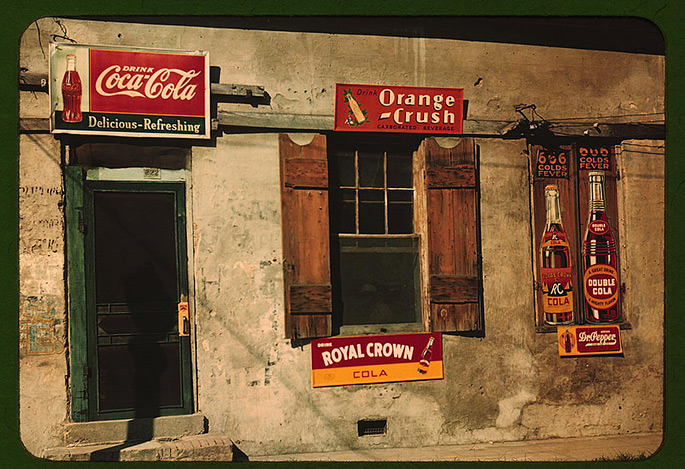
\includegraphics[width=.95\textwidth]{cola-public-domain-photo-p} %{CS0031}
\caption{Coca-Cola Werbung 1940 \cite{CocaCola1940}.}
\label{fig:CocaCola}
\end{figure}



\section{\emph{Let Them Float!}}

Das Platzieren von Abbildungen und Tabellen gehört zu den
schwierigsten Aufgaben im Schriftsatz, weil diese meist viel Platz
benötigen und häufig nicht auf der aktuellen Seite im laufenden
Text untergebracht werden können. Diese Elemente müssen daher an
eine geeignete Stelle auf nachfolgenden Seiten verschoben werden,
was manuell sehr mühsam (jedoch in \emph{Word} beispielsweise unerlässlich) ist.

In \latex funktioniert das weitgehend automatisch, indem
Abbildungen, Tabellen und ähnliche als "`Floating Bodies"'
behandelt werden. Bei der Positionierung dieser Elemente wird
versucht, einerseits im Textfluss möglichst wenig Leer\-raum
entstehen zu lassen und andererseits die Abbildungen und Tabellen
nicht zu weit von der ursprünglichen Textstelle zu entfernen.

Der Gedanke, dass etwa Abbildungen kaum jemals genau an der
ge\-wünsch\-ten Stelle und möglicherweise nicht einmal auf
derselben Seite Platz finden, ist für viele Anfänger aber offenbar sehr
ungewohnt oder sogar beängstigend. Dennoch sollte zunächst einmal
getrost \latex\ diese Arbeit überlassen und \emph{nicht} manuell
eingegriffen werden. Erst am Ende, wenn das gesamte Dokument "`steht"' und
die automatische Platzierung wirklich nicht zufriedenstellend erscheint, sollte (durch gezielte Platzierungsanweisungen
\cite[S.~49]{Oetiker2014}) \textbf{in Einzelfällen} eingegriffen werden.



\section{Captions}

Bei Abbildungen steht der Titel üblicherweise \emph{unten}, bei
Tabellen hingegen -- je nach Konvention -- \emph{oben} (wie in diesem Dokument) 
oder ebenfalls \emph{unten}. In \latex\ erfolgt
auch die Nummerierung der Abbildungen automatisch, ebenso der
Eintrag in das (optionale)
Abbildungsverzeichnis%
\footnote{Ein eigenes Verzeichnis der Abbildungen am Anfang des Dokuments
ist zwar leicht erstellt, in einer Abschlussarbeit aber (und eigentlich
überall sonst auch) überflüssig. Man sollte es daher weglassen.}
am Beginn des Dokuments.

Die Markierung der Captions%
\footnote{Ausnahmsweise wird das Wort "`Caption"' im Folgenden
ohne deutsche Übersetzung verwendet.} erfolgt in \latex mithilfe
der \verb!\label{}! Anweisung, die unmittelbar auf die
\verb!\caption{}! Anweisung folgen muss:
%
\begin{LaTeXCode}[numbers=none]
\begin{figure}
\centering
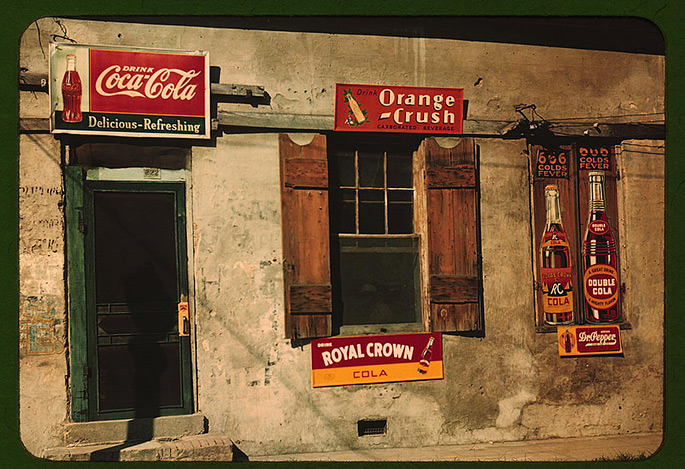
\includegraphics[width=.95\textwidth]{cola-public-domain-photo-p}
\caption{Coca-Cola Werbung 1940 \cite{CocaCola1940}.}
\label{fig:CocaCola}
\end{figure}
\end{LaTeXCode}
%
Der Name des Labels (\texttt{fig:CocaCola}) kann beliebig gewählt werden. 
Die Kennzeichnung \texttt{fig:} ist (wie in Abschn.\ \ref{sec:querverweise} 
erwähnt) nur eine nützliche Hilfe, um beim Schreiben verschiedene Arten 
von Labels besser unterscheiden zu können.

Die Länge der Captions kann dabei sehr unterschiedlich sein. Je
nach Anwendung und Stil ergibt sich manchmal eine sehr kurze
Caption (Abb.~\ref{fig:CocaCola}) oder eine längere
(Abb.~\ref{fig:ibm360}).
Man beachte, wie bei kurzen Captions ein
zentrierter Satz und bei langen Captions ein Blocksatz verwendet
wird (\latex macht das automatisch).
Captions sollten \emph{immer} mit einem Punkt abgeschlossen sein.%
\footnote{Kurioserweise verlangen manche Anleitungen
genau das Gegenteil, angeblich, weil beim klassischen Bleisatz 
die abschließenden Punkte im Druck häufig "`weggebrochen"' sind. 
Das kann man glauben oder nicht, im Digitaldruck 
spielt es jedenfalls keine Rolle.}

\begin{figure}
\centering
\FramePic{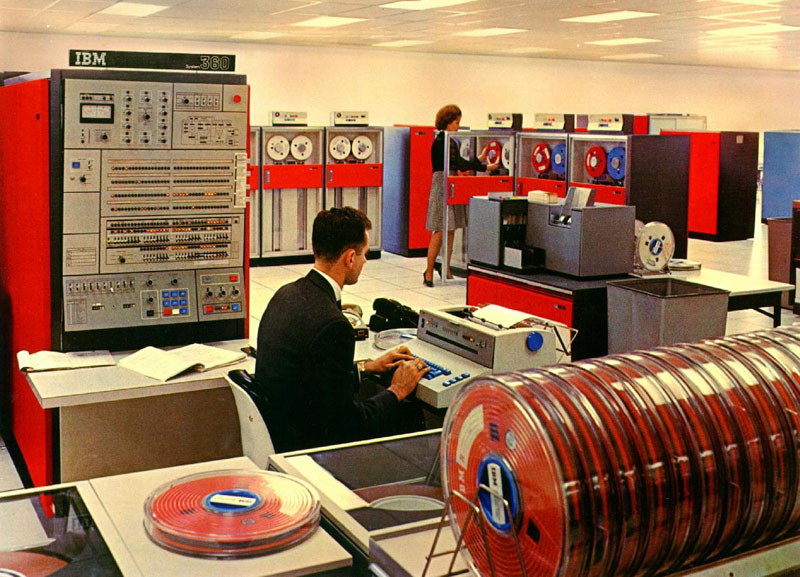
\includegraphics[width=.85\textwidth]{ibm-360-color}}  %{CS1065}}
\caption{Beispiel für einen langen Caption-Text. \textsc{Univac}
brachte 1961 mit dem Modell 751 den ersten Hochleistungsrechner
mit Halbleiterspeicher auf den Markt. Von diesem Computer wurden
in den U.S.A.\ bereits im ersten Produktionsjahr über fünfzig
Exemplare verkauft, vorwiegend an militärische Dienststellen,
Versicherungen und Großbanken. Die Ablöse erfolgte zwei Jahre
später durch das zusammen mit \textsc{Sperry} entwickelte Modell 820.
Das klingt vielleicht plausibel, ist aber völliger Unsinn, und das
Bild zeigt in Wirklichkeit eine System/360 Anlage von IBM. 
Bildquelle~\cite{IBM360}.} 
\label{fig:ibm360}
\end{figure}





\section{Abbildungen}

Für die Einbindung von Grafiken in \latex wird die Verwendung des Stan\-dard-Pakets
\texttt{graphicx} \cite{Carlisle2014} empfohlen 
(wird durch das \texttt{hagenberg}-Paket bereits eingebunden). 
Mit dem aktuell verwendeten Workflow (\texttt{pdflatex})
können Bild- bzw.\ Grafikformate ausschließlich 
in folgenden Formaten eingebunden werden:
%
\begin{itemize}
	\item \textbf{PNG}: für Grau-, S/W- und Farb-Rasterbilder (bevorzugt),
	\item \textbf{JPEG}: für Fotos (wenn nicht anders vorhanden),
	\item \textbf{PDF}: für Vektorgrafiken (Illustrationen, Strichzeichnungen etc.).
\end{itemize}
%
Bei Rasterbildern sollte wenn möglich PNG verwendet werden, weil die darin 
enthaltenen Bilder verlustfrei komprimiert sind und daher keine sichtbaren Kompressionsartefakte
aufweisen. Im Gegensatz dazu sollte JPEG nur dann verwendet werden, wenn das Originalmaterial
(Foto) bereits in dieser Form vorliegt.


\subsection{Wo liegen die Grafikdateien?} 

Die Bilder werden üblicherweise in einem Unterverzeichnis (oder in mehreren Unterverzeichnissen) abgelegt,
im Fall dieses Dokuments in \nolinkurl{images/}.
Dazu dient die folgende Anweisung
am Beginn des Hauptdokuments \nolinkurl{_DaBa.tex} (\sa\ Anhang \ref{app:latex}):
%
\begin{quote}
\verb!\graphicspath{{images/}}!
\end{quote}
%
Der (zum Hauptdokument relative) Pfad \texttt{graphicspath} kann innerhalb des
Dokuments jederzeit geändert werden, was durchaus nützlich ist, wenn
\zB\ die Grafiken einzelner Kapitel getrennt in entsprechenden Verzeichnissen
abgelegt werden sollen.
Die Größe der Abbildung im Druck kann durch Vorgabe einer bestimmten
Breite oder Höhe oder eines Skalierungsfaktors gesteuert werden, {\zB}:
%
\begin{quote}
\verb!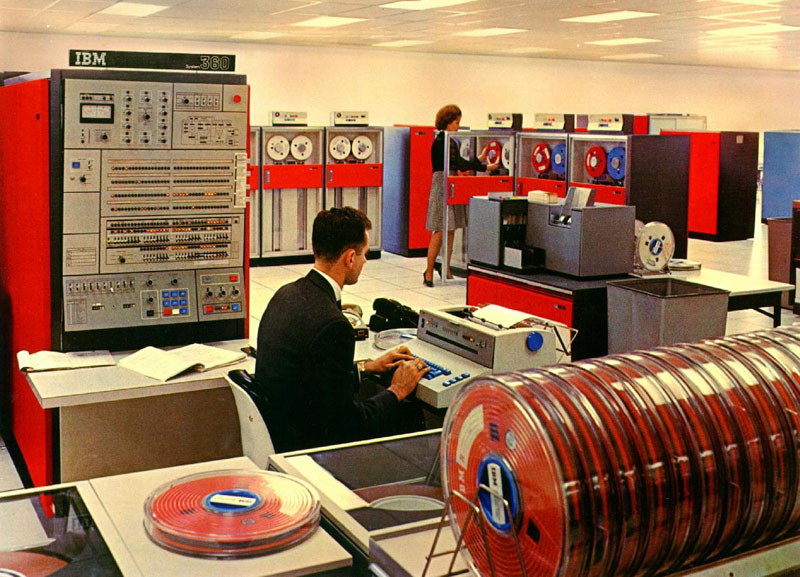
\includegraphics[width=.85\textwidth]{ibm-360-color}! \\
\verb!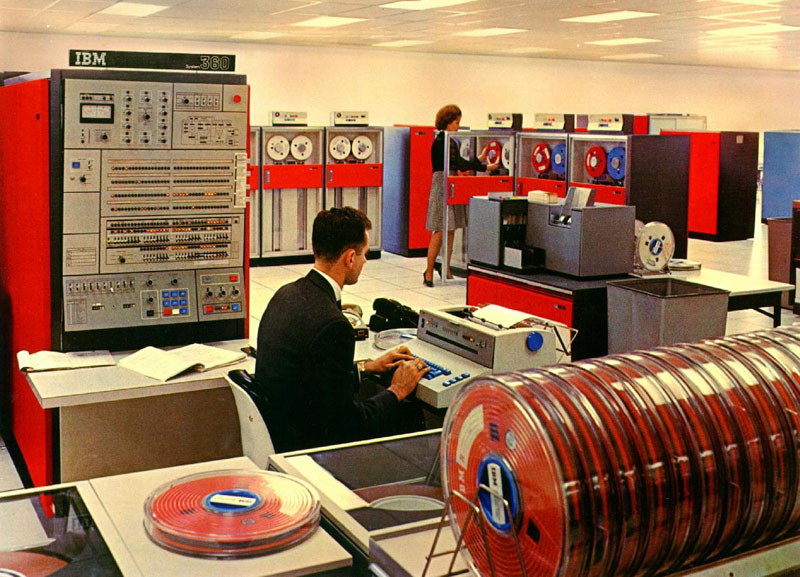
\includegraphics[scale=1.5]{ibm-360-color}!
\end{quote}
%
Man beachte, dass dabei die Dateiendung nicht explizit angegeben werden muss. 
Das ist \va\ dann praktisch, wenn verschiedene Workflows mit jeweils
unterschiedlichen Dateitypen verwendet werden.


\subsection{Grafiken einrahmen} 

Mit dem Makro \verb!\FramePic{}! (definiert in \texttt{hgb.sty}) kann optional ein dünner 
Rahmen rund um die Grafik erzeugt werden, \zB:
%
\begin{quote}
\verb!\FramePic{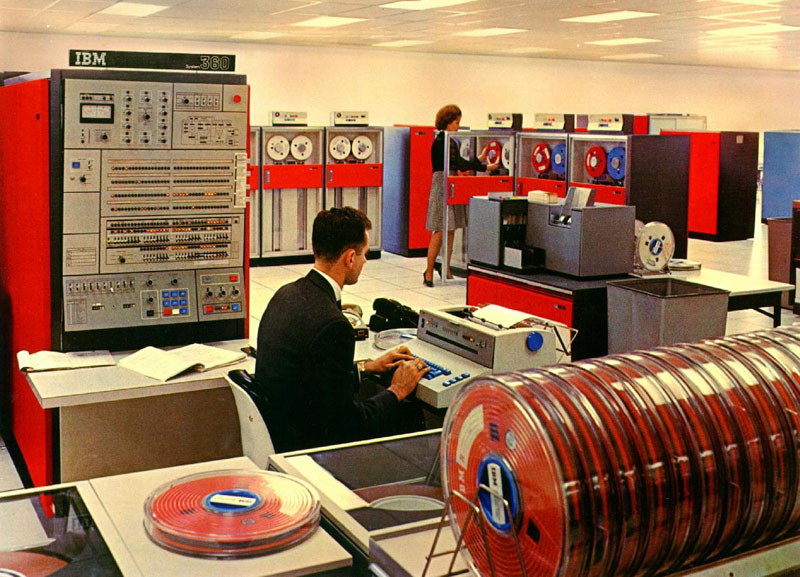
\includegraphics[height=50mm]{ibm-360-color}}!
\end{quote}
%
Das wird üblicherweise nur bei Rasterbildern nötig sein, insbesondere wenn sie zum Rand hin sehr hell sind
und ohne Rahmen nicht vom Hintergrund abgrenzbar wären.

\subsection{Rasterbilder (Pixelgrafiken)}

Generell sollten Bilder bereits vorher so aufbereitet werden,
dass sie später beim Druck möglichst wenig an Qualität verlieren.
Es empfiehlt sich daher, die Bildgröße (Auflösung) bereits im Vorhinein
(\zB mit \emph{Photoshop})
richtig einzustellen.
Brauchbare Auflösungen bezogen auf die endgültige Bildgröße sind:
%
\begin{itemize}
  \item \textbf{Farb- und Grauwertbilder:} 150--300 dpi
  \item \textbf{Binärbilder (Schwarz/Weiß):} 300--600 dpi
\end{itemize}
%
Eine wesentlich höhere Auflösung macht aufgrund der beim Laserdruck notwendigen
Rasterung keinen Sinn, auch bei 1200 dpi-Druckern.
Speziell \emph{Screen\-shots} sollten nicht zu klein dargestellt werden,
da sie sonst schlecht lesbar sind (max.\ 200 dpi, besser 150 dpi).
Dabei ist zu bedenken, dass die Arbeit auch als Kopie in allen
Details noch gut lesbar sein sollte.

\subsubsection{JPEG-Problematik}

In der Regel sollten Bilder, die für den Einsatz in
Druckdokumenten gedacht sind, nicht mit verlustbehafteten
Kompressionsverfahren abgespeichert werden. Insbesondere sollte die Verwendung
von JPEG möglichst vermieden werden, auch wenn viele Dateien dadurch
wesentlich kleiner werden. 
Eine Ausnahme ist, wenn die Originaldaten nur in JPEG vorliegen und für die 
Einbindung nicht bearbeitet oder verkleinert wurden. Ansonsten sollte immer
PNG verwendet werden.

Besonders gerne werden farbige \textbf{Screenshots} einer JPEG-Kompression%
\footnote{Das JPEG-Verfahren ist für natürliche Fotos konzipiert und dafür auch gut geeignet,
seine undifferenzierte Verwendung ist aber zu einer globalen Plage geworden.}
unterzogen, obwohl deren verheerende Folgen auch für jeden Laien sichtbar sein sollten
(Abb.~\ref{fig:jpeg-pfusch}).

\begin{figure}
\centering\small
\begin{tabular}{cc}
\FramePic{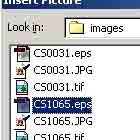
\includegraphics[width=0.45\textwidth]{screenshot-dirty}} &		% JPEG file
\FramePic{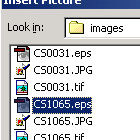
\includegraphics[width=0.45\textwidth]{screenshot-clean}} \\	% PNG file
(a) & (b) 
\end{tabular}
\caption{Typischer JPEG-Pfusch. Screenshots und ähnliche im Original
verfügbare Rasterbilder sollten für Druckdokumente \emph{keinesfalls} mit
JPEG komprimiert werden. Das Ergebnis~(a) sieht gegenüber dem
unkomprimierten Original~(b) nicht nur schmutzig aus, sondern wird
im Druck auch schnell unleserlich.} 
\label{fig:jpeg-pfusch}
\end{figure}



\subsection{Vektorgrafiken}

Für schematische Abbildungen (\zB Flussdiagramme, Entity-Relationship-Diagramme
oder sonstige strukturelle Darstellungen) sollten unbedingt
Vektorgrafiken (PDF) verwendet werden. % (\zB Abb.~\ref{fig:latex-pdf-workflow}).
Gerasterte Grafiken, wie sie üblicherweise als GIF- oder PNG-Dateien
auf Webseiten vorliegen, haben in einem Druckdokument nichts zu suchen, notfalls
müssen sie mit einem entsprechenden Werkzeug \emph{neu} gezeichnet werden (natürlich
unter Angabe der ursprünglichen Quelle).

In diesem Fall kommt als Datenformat nur PDF %(oder EPS im DVI-PS-Workflow) 
in Frage,
dieses bietet sich aber auch in anderen Umgebungen als universelles
Vektor-Format an.
Zur Erstellung von PDF-Vektorgrafiken wird ein geeignetes
Grafikprogramm, \zB\ %\emph{Freehand} von \emph{Macromedia} oder
\emph{Illustrator} von \emph{Adobe} benötigt.
Manche gängigen Grafikprogramme 
unterstützen allerdings keinen direkten Export von PDF-Dateien
oder erzeugen unsaubere Dateien. Vor der Entscheidung
für eine bestimmte Zeichensoftware sollte das im Zweifelsfall
ausprobiert werden.
PDF kann im Notfall über einen entsprechenden Druckertreiber erzeugt werden.


\subsubsection{Einbettung von Schriften}

Die Wiedergabe von Textelementen ist abhängig von der auf dem
Computer (oder Drucker) installierten Schriften und der Form der
Schrifteinbettung im Quelldokument. Die korrekte Darstellung am
Bildschirm eines Computers bedeutet nicht, dass dasselbe Dokument
auf einem anderen Computer oder Drucker genau so dargestellt wird.
Dieser Umstand ist besonders wichtig, wenn Druckdokumente online
zur Verfügung gestellt werden. Kontrollieren Sie daher genau, ob
die innerhalb Ihrer Grafiken verwendeten Schriften auch exakt wie
beabsichtigt im Ausdruck aufscheinen.


\subsubsection{Strichstärken -- \emph{Hairlines} vermeiden!}

In Grafik-Programmen wie \emph{Freehand} und \emph{Illustrator},
die sich im Wesentlichen an der \emph{PostScript}-Funktionalität
orientieren, ist es möglich, Linien bzgl.\ ihrer Stärke als
"`Hairline"' zu definieren. Im zugehörigen \emph{PostScript}-Code
wird dies als \texttt{linewidth} mit dem Wert \texttt{0} ausgedrückt und
sollte am Ausgabegerät "`möglichst dünne"' Linien ergeben. 
Das Ergebnis ist ausschließlich vom jeweiligen Drucker
abhängig und somit kaum vorhersagbar.
\textbf{Fazit:} Hairlines vermeiden und stattdessen immer konkrete
Strichstärken ($\geq 0.25\,\mathrm{pt}$) einstellen!





\subsection{\tex-Schriften auch in Grafiken?}
\label{sec:tex-schriften-in-grafiken}

Während bei Abbildungen, die mit externen
Grafik-Programmen erzeugt werden, meist mit ähnlich aussehende
Schriften (wie \emph{Times-Roman} oder \emph{Garamond}) Abhilfe schaffen,
besteht bei Puristen oft der verständliche Wunsch, die 
\emph{Computer-Modern} (CM) Schriftfamilie von {\tex}/{\latex} auch
innerhalb von eingebetteten Grafiken einzusetzen.

\subsubsection{\emph{BaKoMa}-Schriften (TrueType)}

Glücklicherweise stehen einige Portierungen von CM als {\em
TrueType}-Schriften zur Verfügung, die auch in herkömmlichen
DTP-Anwendungen unter \emph{Windows} und \emph{Mac~OS} verwendet werden
können. Empfehlenswert ist \zB\ die \emph{BaKoMa Fonts
Collection}\footnote{Von Basil K.\ Malyshev -- die BaKoMa-Fonts
liegen dieser Vorlage bei, ansonsten finden sie sich \zB\ unter
\url{www.ctan.org/tex-archive/fonts/cm/ps-type1/bakoma/}.}, die
neben den CM-Standardschriften auch die mathematischen Schriften
der AMS-Familie ent\-hält und zudem kostenfrei ist. Natürlich
müssen die TrueType Schriften vor der Verwendung zunächst auf dem
eigenen PC installiert werden. 
%Ein Beispiel für eine in {\em
%Freehand} erzeugte Grafik mit CM-Schriften findet sich in
%Abb.~\ref{fig:latex-pdf-workflow} (Seite
%\pageref{fig:latex-pdf-workflow}).

\subsubsection{\emph{Latin Modern Roman} Fonts (OpenType)}

Eine Alternative dazu sind die "`LM-Roman"'%
\footnote{\url{http://www.gust.org.pl/projects/e-foundry/latin-modern}}
 Open-Type Schriften, die speziell für die Verwendung im Umfeld von \latex\ entwickelt wurden.
Sie sind auch Teil der MikTeX-Installation.%
\footnote{\zB unter \url{C:/Program Files (x86)/MikTeX 2.9/fonts/opentype/public/lm/}}
Diese Schriften enthalten \ua\ Zeichen mit Umlauten und sind daher auch für deutsche Texte recht
bequem zu verwenden.



\subsection{Für Gourmets: Grafiken mit \latex-Overlays}
\label{sec:GraphicOverlays}

Bisweilen ist es erforderlich, ein bestehendes Bilder oder eine Grafik mit 
\latex-eigenen (Vektor-)Elementen zu überlagern, \zB\ für Markierungen
oder Beschriftungen. Ein typisches Beispiel ist in Abb.~\ref{fig:overpic-example}
gezeigt, wo eine mit \emph{Mathematica} generierte PDF-Grafik
mit mathematischen Elementen annotiert wird.


\begin{figure}
\centering\small
%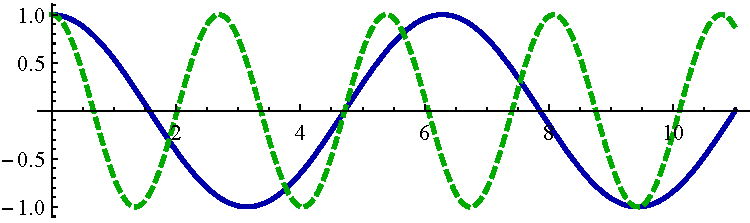
\includegraphics[width=0.85\textwidth]{mathematica-example}
\vspace*{3mm}
\begin{overpic}[width=0.85\textwidth]{mathematica-example}
	\put(101,14){$x$}%
	\put(4,31){$f(x)$}%
	\put(29.5,28){\line(1,1){2}}%
	{\color{green!70!black}\put(29.5,28){\circle*{2.0}}}%
	\put(32,30){$\cos(\frac{7}{3} x)$}%
	\put(59,28){\line(1,1){2}}%
	{\color{blue!70!black}\put(59,28){\circle*{2.0}}}%
	\put(61.5,30){$\cos(x)$}%
\end{overpic}
\caption{Beispiel für die Verwendung des \texttt{overpic}-Pakets zum Einfügen
von \latex-Elementen über eine importierte Grafik.
In diesem Fall wurden die mathematischen Elemente $x$, $f(x)$, $\cos(x)$ und $\smash{\cos(\frac{7}{3} x)}$
sowie zwei diagonale Geraden und gefüllte (färbige) Kreise eingefügt.
Darunter liegt die Vektor\-grafik \texttt{mathematica-example.pdf}.}
\label{fig:overpic-example}
\end{figure}



Dazu wird das \texttt{overpic}-Paket\footnote{\url{https://www.ctan.org/pkg/overpic}}
verwendet und zum Importieren der Grafik anstelle von \verb!\includegraphics!
die Umgebung \verb!\begin{overpic}! \ldots \verb!\end{overpic}! verwendet 
(mit ähnlicher Syntax):

\begin{LaTeXCode}[numbers=none]
\begin{overpic}[width=0.85\textwidth]{mathematica-example}
	\put(101,14){$x$}%
	\put(4,31){$f(x)$}%
	\put(29.5,28){\line(1,1){2}}%
	...
\end{overpic}
\end{LaTeXCode}

Die \texttt{overpic}-Umgebung bildet gleichzeitig eine \texttt{picture}-Umgebung, 
in der \latex-Zeichenanweisungen (wie \verb!\put! u.ä.) platziert werden
können, wie in obigem Beispiel gezeigt.\footnote{Die Standard-Zeichenanweisungen
in \latex sind ziemlich restriktiv, weshalb hier zusätzlich das \texttt{pict2e}-Paket
(\url{https://www.ctan.org/pkg/pict2e}) verwendet wird.}
Die $x/y$-Positionen sind in Prozent der Bildbreite angegeben.
Weitere Details finden sich im Quelltext.





\subsection{Abbildungen mit mehreren Elementen}

Werden mehrere Bilder oder Grafiken zu einer Abbildung zusammengefasst, 
wird üblicherweise eine gemeinsame Caption verwendet, wie in Abb.~\ref{fig:Bearings}
dargestellt. Im Text könnte ein Verweis auf einen einzelnen Teil der Abbildung, etwa das 
einreihige Rollenlager in Abb.~\ref{fig:Bearings}\,(c), so aussehen:
%
\begin{itemize}
\item[] \verb!Abb.~\ref{fig:Bearings}\,(c)! 
\end{itemize}
%
Für kompliziertere Abbildungen sollte die Verwendung des 
\texttt{subfig}-Pakets \cite{Cochran05} in Betracht gezogen werden.


\subsection{Quellenangaben in Captions}
\label{sec:QuellenangabenInCaptions}

Wenn Bilder, Grafiken oder Tabellen aus anderen Quellen verwendet werden, dann 
muss ihre Herkunft in jedem Fall klar ersichtlich gemacht werden, und zwar am 
besten direkt in der Caption.
Wird beispielsweise eine Grafik aus einem Buch oder einer sonstigen 
zitierfähigen Publikation verwendet, dann sollte diese in das Literaturverzeichnis 
aufgenommen und wie üblich mit
\verb!\cite{..}! zitiert werden, wie in Abb.\ \ref{fig:Bearings} demonstriert. 
Weitere Details zu dieser Art von Quellenangaben finden sich in 
Kap.\ \ref{cha:Literatur} (insbes.\ Abschnitt \ref{sec:KategorieOnline}).

\begin{figure}
\centering\small
\setlength{\tabcolsep}{0mm}	% alle Spaltenränder auf 0mm
\begin{tabular}{c@{\hspace{12mm}}c} % mittlerer Abstand = 12mm
  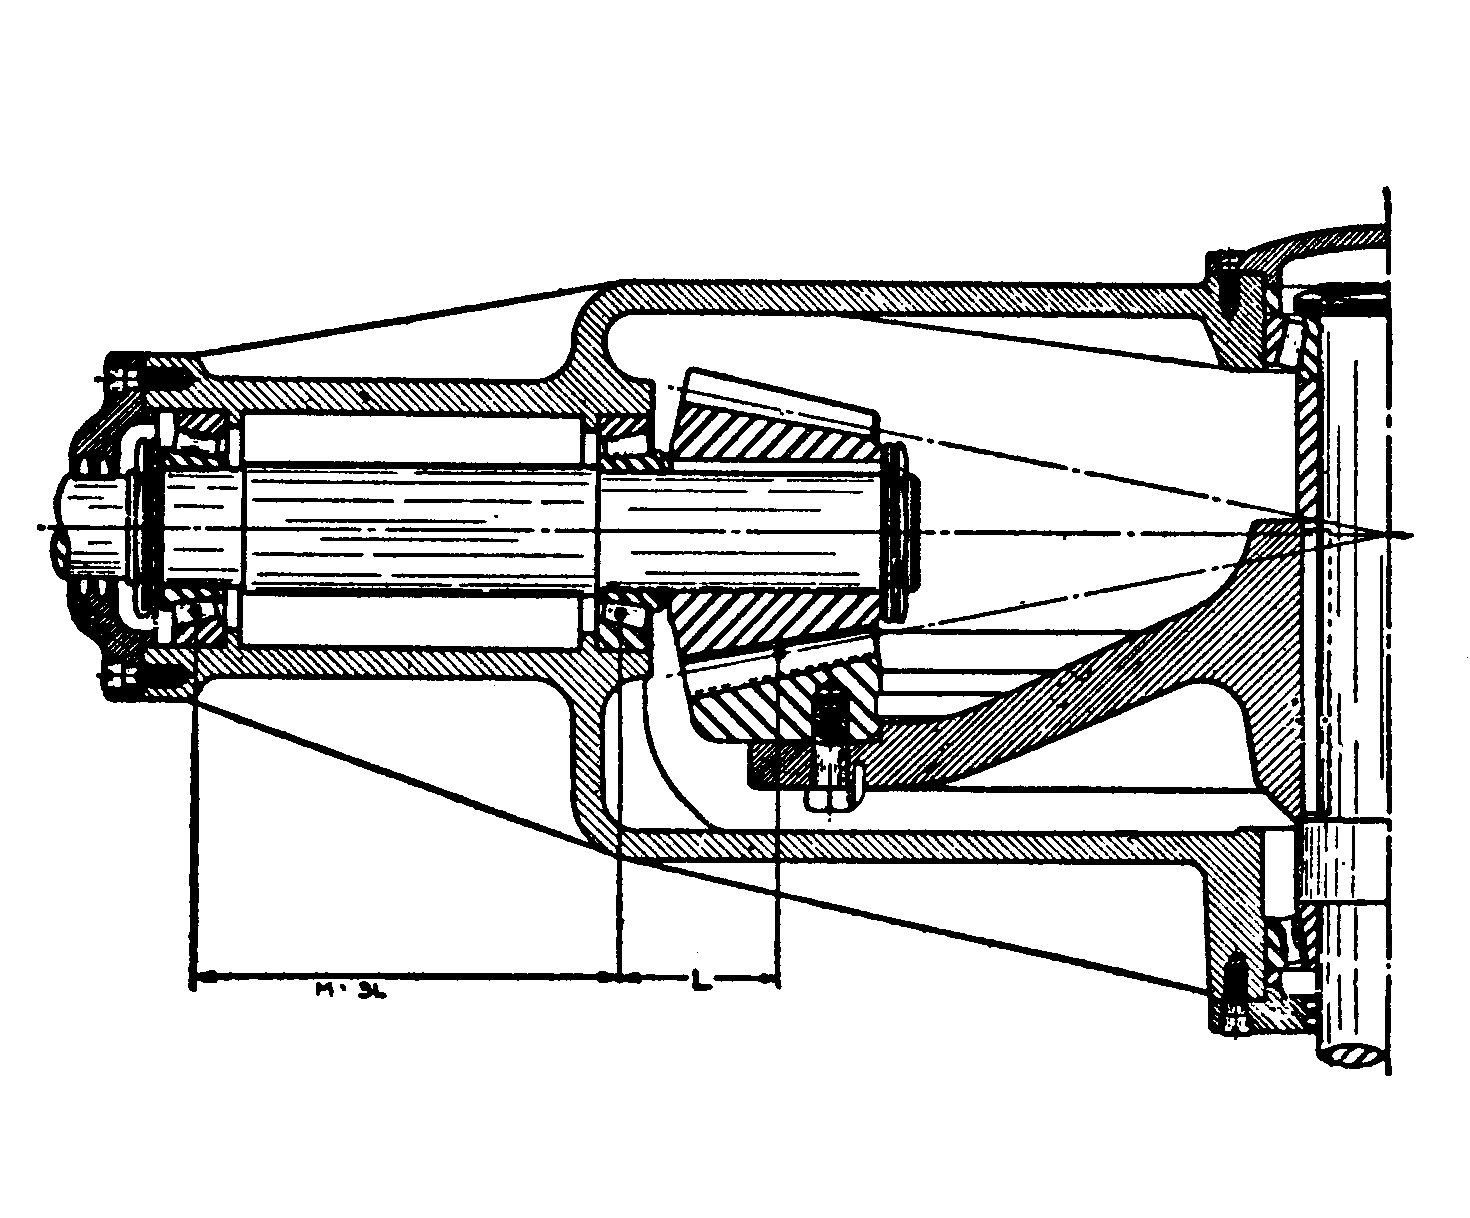
\includegraphics[width=.45\textwidth]{overhang-mounting} &
  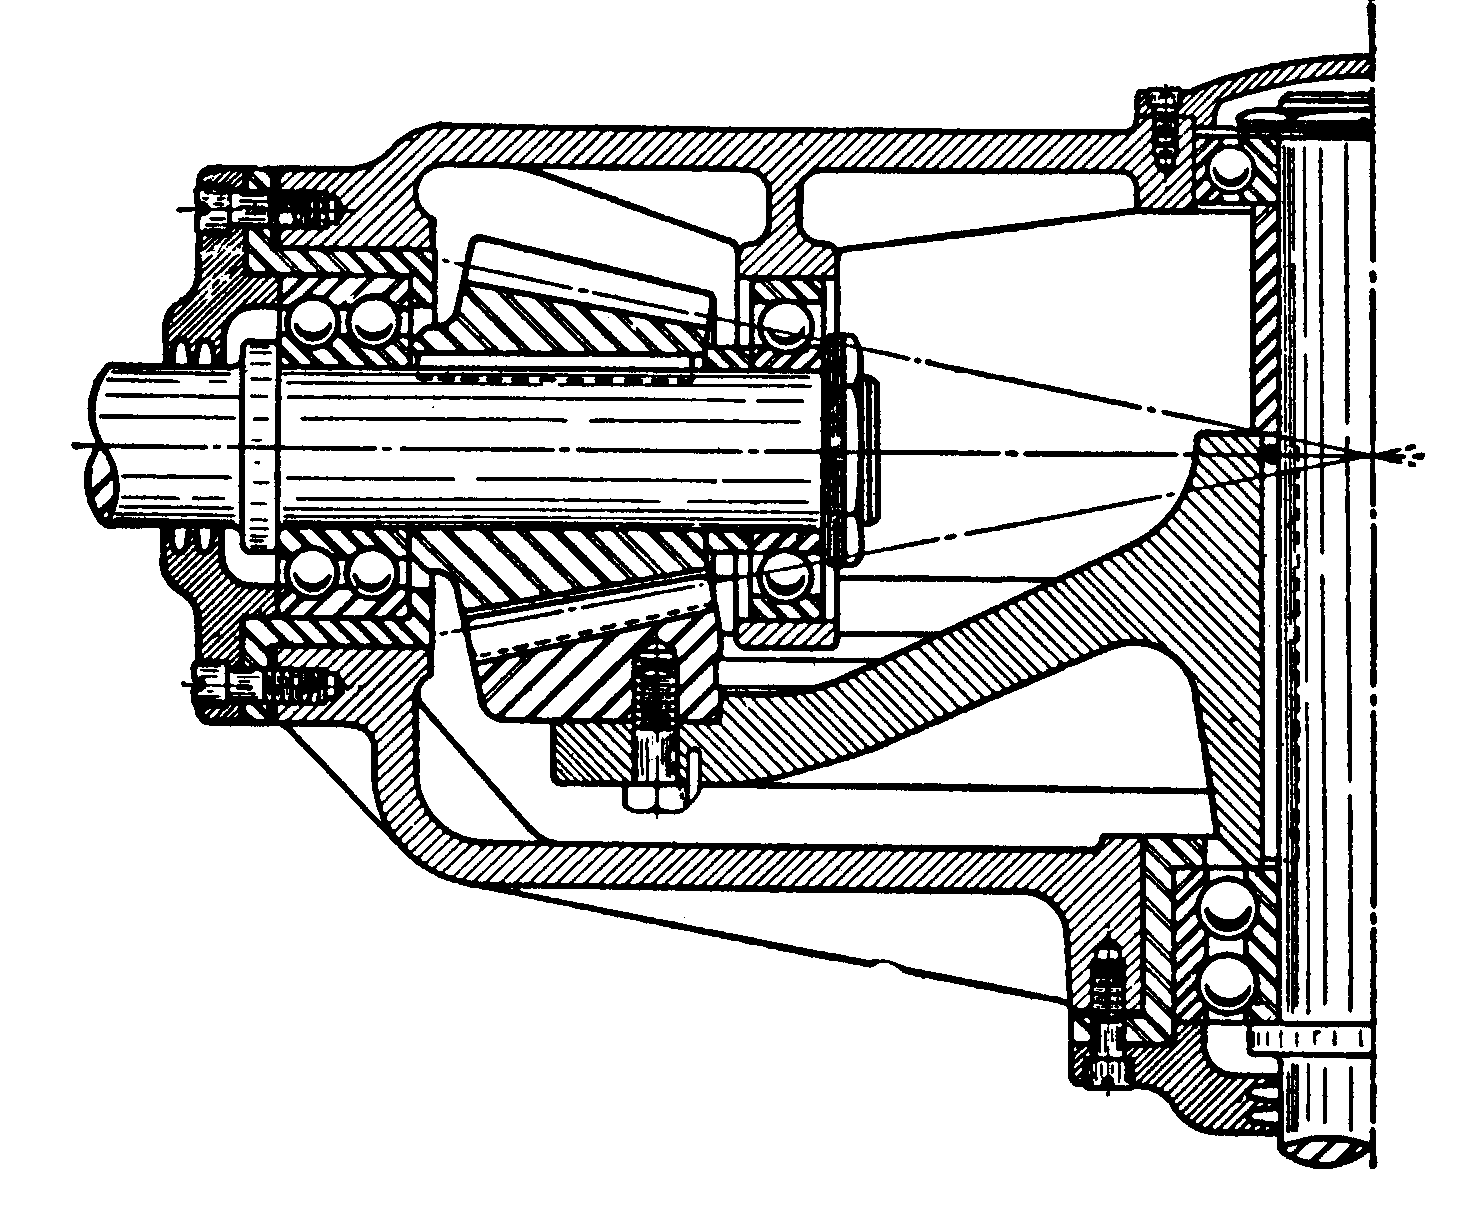
\includegraphics[width=.45\textwidth]{straddle-mounting} \\
  (a) & (b)
\\[4pt]	%vertical extra spacing (4 points)
  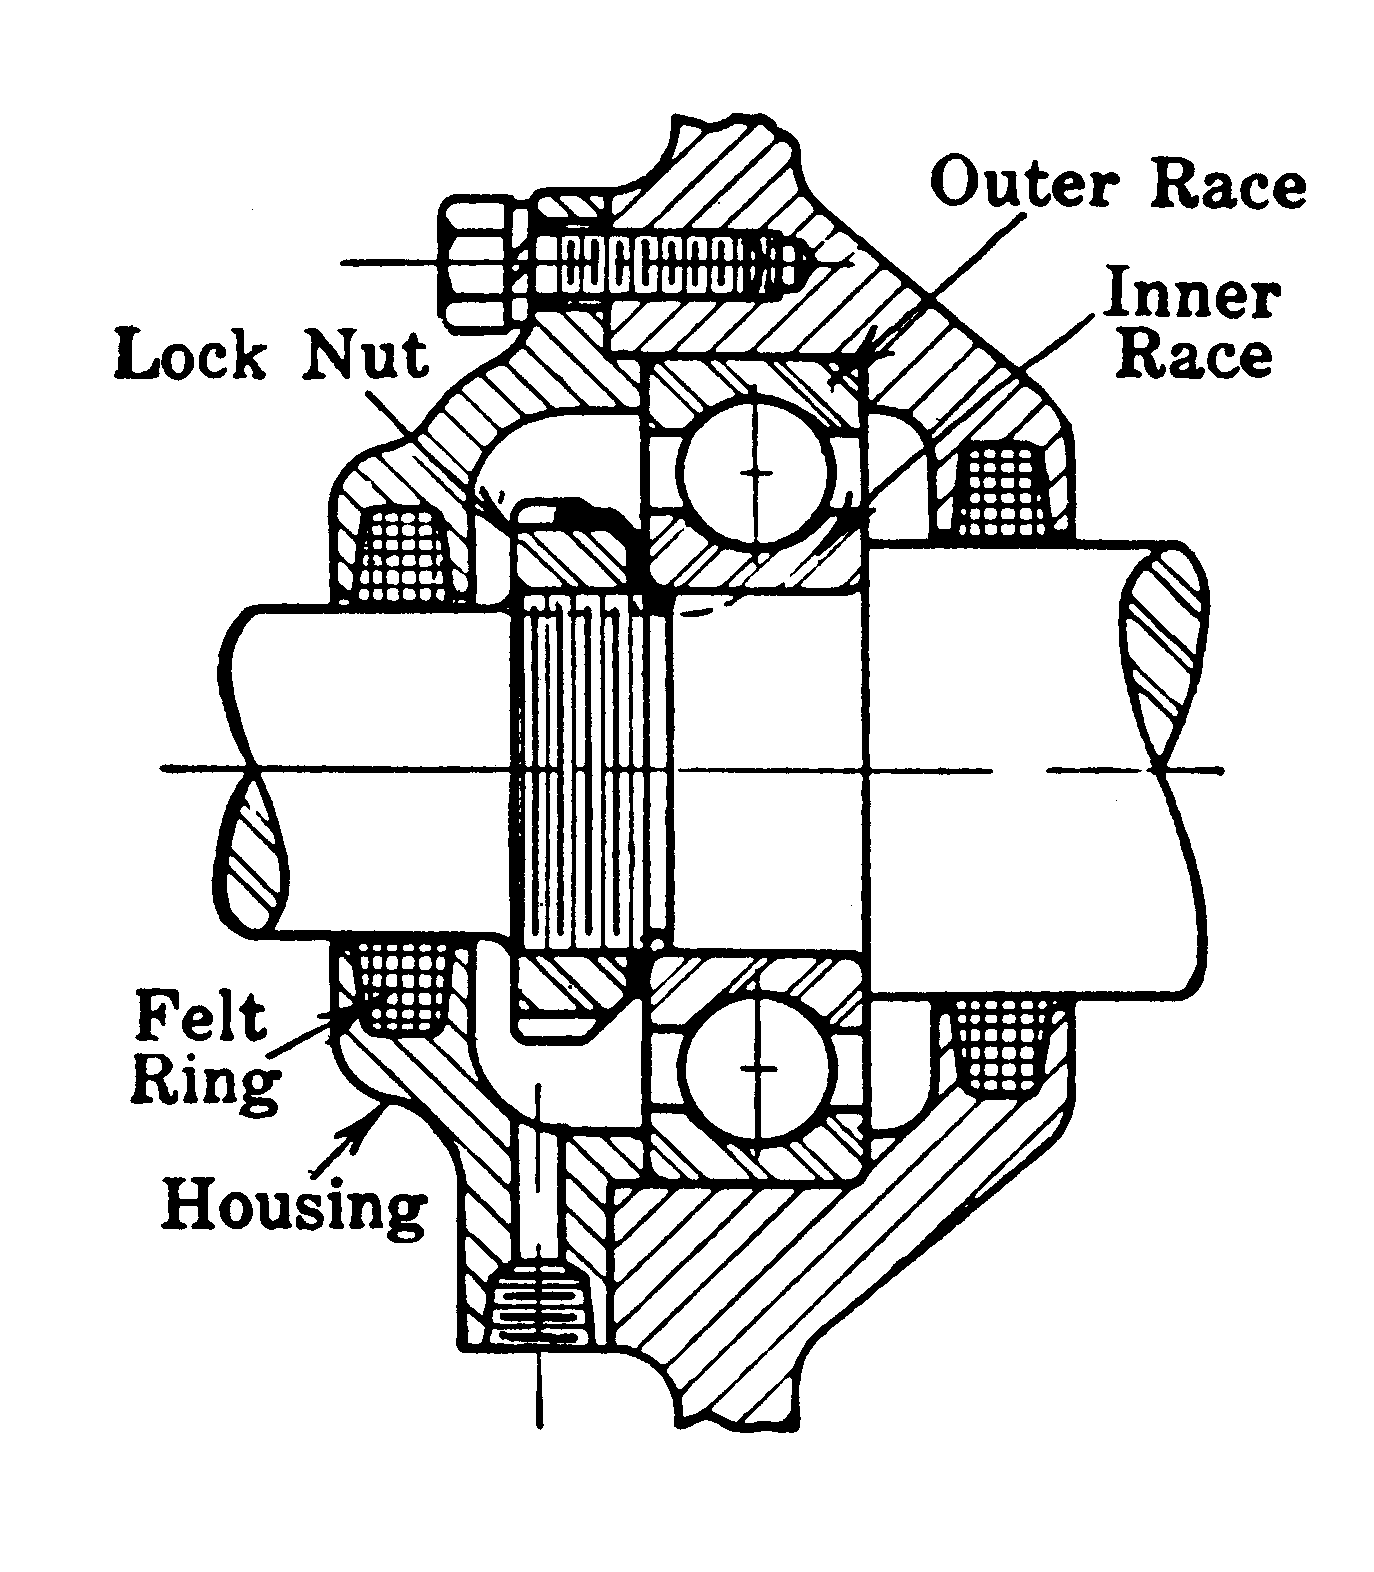
\includegraphics[width=.45\textwidth]{ball-bearing-1} &
  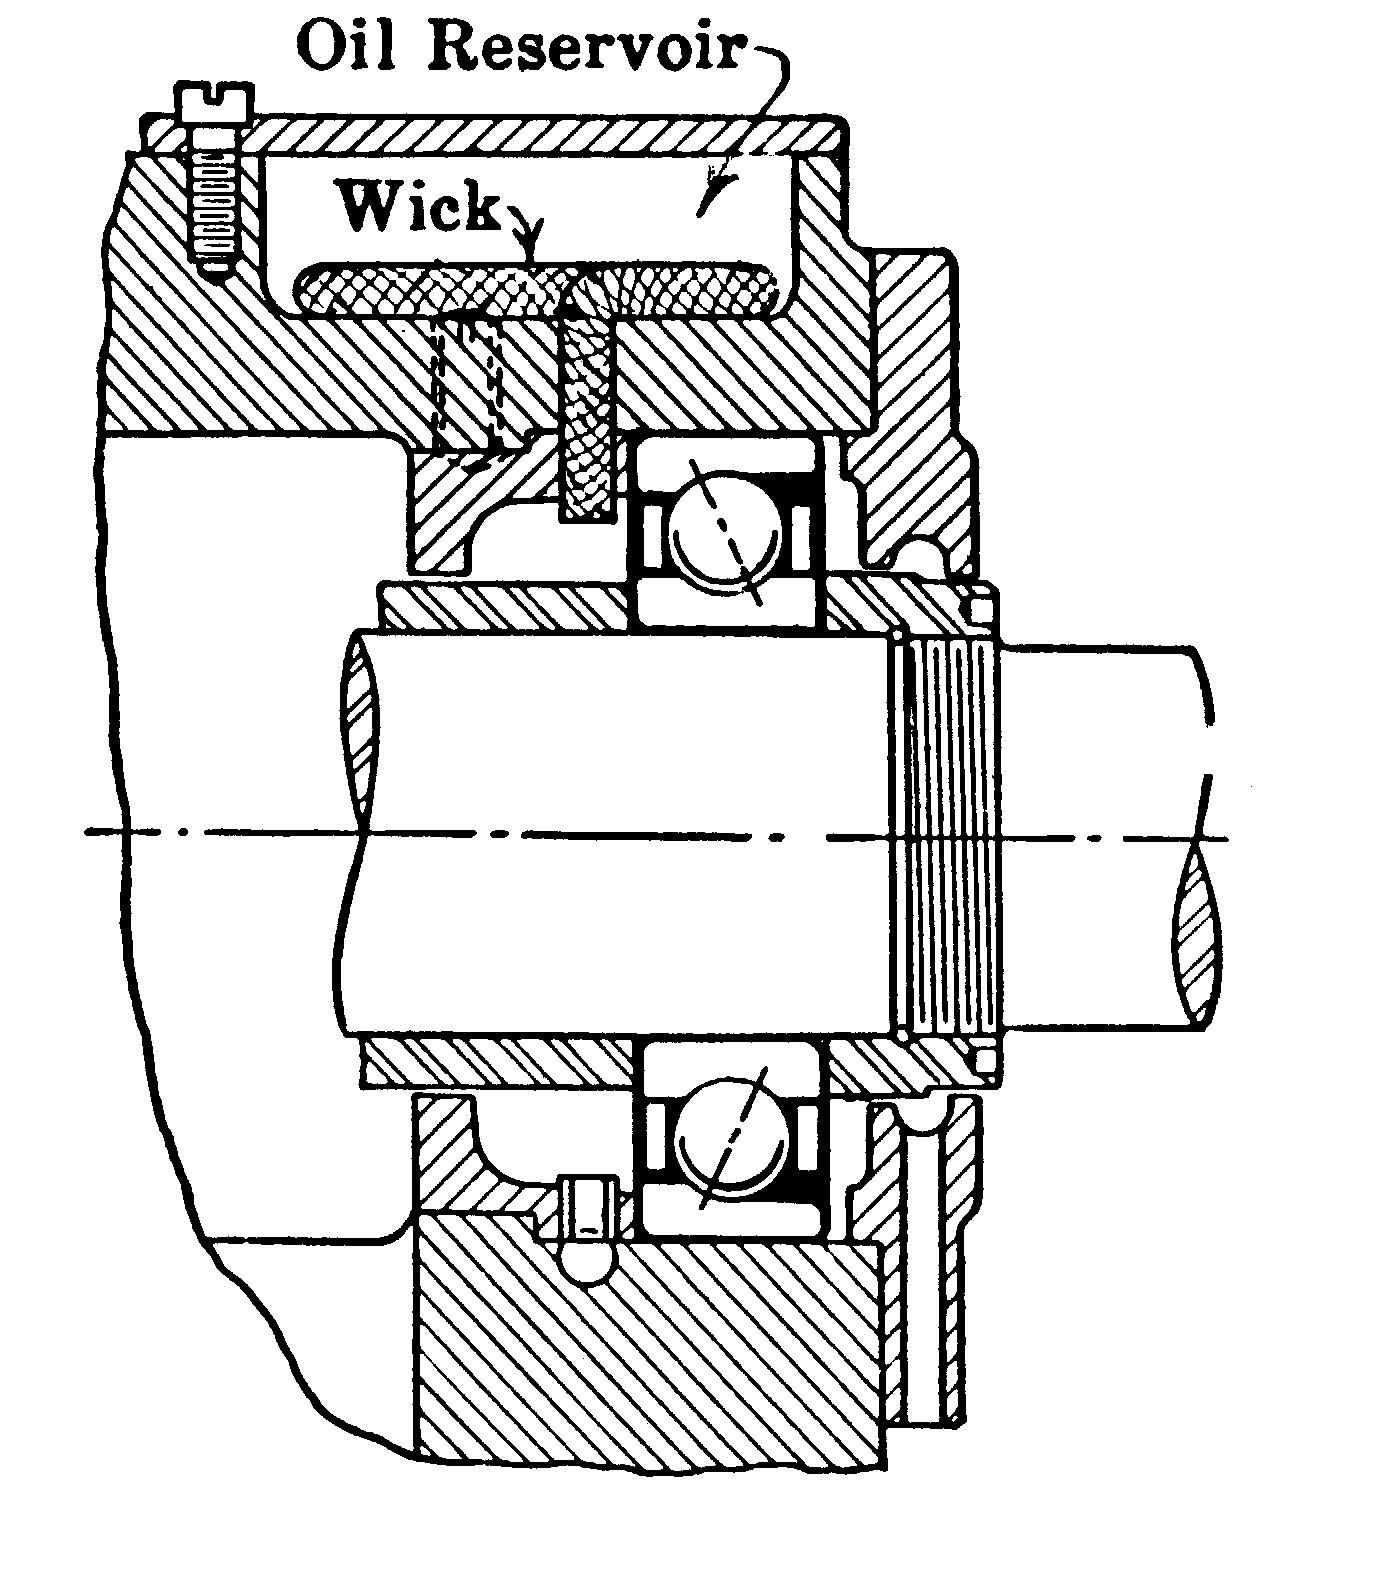
\includegraphics[width=.45\textwidth]{ball-bearing-2} \\
  (c) & (d)
\end{tabular}
%
\caption{Diverse Maschinenelemente als Beispiel für eine
Abbildung mit mehreren Elementen.
Overhang Mounting (a), Straddle Mounting (b),
einreihiges Rollenlager (c), Schmierung von Rollenlagern (d).
Die Abbildung verwendet im oberen Teile eine $2 \times 2$
Tabelle (\texttt{tabular}), in der die Breite der Spaltenränder 
gesondert spezifiziert ist (Details finden sich im Quelltext).
Bildquelle~\cite{Faires34}.
}
\label{fig:Bearings}
\end{figure}




\section{Tabellen}

Tabellen werden häufig eingesetzt um numerische Zusammenhänge, Testergebnisse
etc.\ in übersichtlicher Form darzustellen.
Ein einfaches Beispiel ist Tab.~\ref{tab:processors}, der \latex-Quelltext dazu
findet sich in Prog.~\ref{prog:processors-source}.


\begin{table}
\caption{Prozessor-Familien im Überblick.}
\label{tab:processors}
\centering
\setlength{\tabcolsep}{5mm}	% separator between columns
\def\arraystretch{1.25}			% vertical stretch factor (Standard = 1.0)
\begin{tabular}{|r||c|c|c|} \hline
& \emph{PowerPC} & \emph{Pentium} & \emph{Athlon} \\
\hline\hline
Manufacturer & Motorola & Intel & AMD \\
\hline
Speed & high & medium & high   \\
\hline
Price & high & high   & medium \\
\hline
\end{tabular}
\end{table}

\begin{program}
% place caption consistently either at the top or bottom:
\caption{\latex\ Quelltext zu Tab.~\ref{tab:processors}.
Die Erzeugung des dargestellten Listings selbst ist in Abschn.\ \ref{sec:programmtexte} beschrieben.}
\label{prog:processors-source}
%
\begin{LaTeXCode}[numbers=none]
\begin{table}
	\caption{Prozessor-Familien im Überblick.}
	\label{tab:processors}
	\centering
	\setlength{\tabcolsep}{5mm}	% separator between columns
	\def\arraystretch{1.25}		% vertical stretch factor
	\begin{tabular}{|r||c|c|c|} 
		\hline
		& \emph{PowerPC} & \emph{Pentium} & \emph{Athlon} \\
		\hline
		\hline
		Manufacturer & Motorola & Intel & AMD \\
		\hline
		Speed & high & medium & high   \\
		\hline
		Price & high & high   & medium \\
		\hline
	\end{tabular}
\end{table}
\end{LaTeXCode}
%
\end{program}

Manchmal ist es notwendig, in Tabellen relativ viel Text in engen Spalten
unter zu bringen, wie in Tab.~\ref{tab:synthesis-techniques}. In diesem Fall
ist es sinnvoll, auf den Blocksatz zu verzichten und gleichzeitig die
strengen Abteilungsregeln zu lockern. Details dazu finden sich im zugehörigen
\latex-Quelltext.


%--------------------------------------------------------------------------------
% Table with narrow columns
%--------------------------------------------------------------------------------
\begin{table}
\caption{Beispiel für eine Tabelle mit mehrzeiligem Text in engen Spalten.
Hier werden die Zeilen für den Blocksatz zu kurz, daher wird linksbündig
gesetzt (im "`Flattersatz"').}
\label{tab:synthesis-techniques}
\centering
\def\rr{\rightskip=0pt plus1em \spaceskip=.3333em \xspaceskip=.5em\relax}
\setlength{\tabcolsep}{1ex}
\def\arraystretch{1.20}
\setlength{\tabcolsep}{1ex}
\small
\begin{english}
\begin{tabular}{|p{0.2\textwidth}|c|p{0.3\textwidth}|p{0.2\textwidth}|}
\hline
   \multicolumn{1}{|c}{\emph{Method}} &
   \multicolumn{1}{|c}{\emph{Implem.}} &
   \multicolumn{1}{|c}{\emph{Features}} &
   \multicolumn{1}{|c|}{\emph{Status}} \\
\hline\hline
   {\rr polygon shading} &
   SW/HW &
   {\rr flat-shaded polygons} &
   \\
\hline
  {\rr flat shading with z-buffer} &
  SW/HW &
  {\rr depth values} &
  \\
\hline
  {\rr goraud shading with z-buffer} &
  SW/HW &
  {\rr smooth shading, simple fog, point light sources} &
  {\rr SGI entry models} \\
\hline
  {\rr phong shading with z-buffer} &
  SW/HW &
  {\rr highlights} &
  \\
\hline
  {\rr texture mapping with z-buffer} &
  SW/HW &
  {\rr surface textures, simple shadows} &
  {\rr SGI high end, flight simulators} \\
\hline
%  {\rr reflection mapping with z-buffer} &
%  SW/HW &
%  {\rr reflections} &
%  {\rr SGI next generation} \\
%\hline
%  {\rr raytracing} &
%  SW &
%  {\rr refraction, real camera model, area light sources with penumbra, realistic material models} &
%  {\rr common ray\-tracers} \\
%\hline
%  {\rr raytracing + global illumination simulation} &
%  SW &
%  {\rr indirect illumination} &
%  \textit{Radiance} \\
%\hline
%  {\rr raytracing + global illumination simulation + dissipating media} &
%  none &
%  {\rr realistic clouds, scattering, ...} &
%  {\rr research} \\
%\hline
\end{tabular}
\end{english}
\end{table}

%--------------------------------------------------------------------------------



\section{Programmtexte}
\label{sec:programmtexte}

Die Einbindung von Programmtexten (source code) ist eine häufige Notwendigkeit,
\va natürlich bei Arbeiten im Bereich der Informatik.

\subsection{Formatierung von Programmcode}
\label{sec:FormatierungVonProgrammcode}

Es gibt für \latex\ spezielle Pakete zur Darstellung von Programmen, die \ua\ auch die automatische Nummerierung der Zeilen vornehmen, insbesondere das \texttt{listings}-Package.%
\footnote{\url{http://www.ctan.org/tex-archive/macros/latex/contrib/listings/}}
Damit sind auch die in Tabelle~\ref{tab:CodeUmgebungen} aufgelisteten Code-Umgebungen 
realisiert.
%
\begin{table}
\caption{In \nolinkurl{hgb.sty} vordefinierte Code-Umgebungen.}
\label{tab:CodeUmgebungen}
\centering
\begin{tabular}{llll}
	\hline
	C (ANSI):   & \verb!\begin{CCode}! & \verb!...! \verb!\end{CCode}! \\
	C++ (ISO):  & \verb!\begin{CppCode}! & \verb!...! \verb!\end{CppCode}! \\
	C\#:   & \verb!\begin{CsCode}! & \verb!...! \verb!\end{CsCode}! \\
	Objective-C:   & \verb!\begin{ObjCCode}! & \verb!...! \verb!\end{ObjCCode}! \\
	Java:       & \verb!\begin{JavaCode}! & \verb!...! \verb!\end{JavaCode}! \\
	JavaScript:  			& \verb!\begin{JsCode}! & \verb!...! \verb!\end{JsCode}! \\
	PHP:  			& \verb!\begin{PhpCode}! & \verb!...! \verb!\end{PhpCode}! \\
	HTML:  			& \verb!\begin{HtmlCode}! & \verb!...! \verb!\end{HtmlCode}! \\
	CSS:  			& \verb!\begin{CssCode}! & \verb!...! \verb!\end{CssCode}! \\
	XML:  			& \verb!\begin{XmlCode}! & \verb!...! \verb!\end{XmlCode}! \\
	\latex:     & \verb!\begin{LaTeXCode}! & \verb!...! \verb!\end{LaTeXCode}! \\
	Generisch:  & \verb!\begin{GenericCode}! & \verb!...! \verb!\end{GenericCode}! \\
	\hline
\end{tabular}
\end{table}
%
Die Verwendung ist äußerst einfach, \zB\ für Quellcode in der Programmiersprache C schreibt man
%
\begin{quote}
\begin{verbatim}
\begin{CCode}
    ... 
\end{CCode}
\end{verbatim}
\end{quote}
%
Der Quellcode innerhalb dieser Umgebungen wird in der jeweiligen Programmiersprache interpretiert, wobei Kommentare erhalten bleiben. Diese Umgebungen können sowohl alleinstehend (im Fließtext) oder innerhalb von Float-Umgebungen (insbes.\ \texttt{program}) verwendet werden. Im ersten Fall wird der Quelltext auch über Seitengrenzen umgebrochen. Mit \verb!/+! ... \verb!+/! ist eine Escape-Möglichkeit nach \latex\ vorgesehen, die \va\ zum Setzen von Labels für Verweise auf einzelne Programmzeilen nützlich ist, \zB\ mit
%
\begin{quote}
\verb!/+\label{ExampleCodeLabel}+/!
\end{quote}
%
Ein Beispiel mit Java ist in Prog.~\ref{prog:CodeExample} gezeigt, wobei der oben angeführte Label in Zeile \ref{ExampleCodeLabel} steht.
Man beachte, dass innerhalb der Kommentare auch mathematischer Text (wie etwa in Zeile \ref{MathInCode} von Prog.~\ref{prog:CodeExample}) stehen kann.


\subsubsection{Nummerierung der Code-Zeilen}

Alle in Tabelle~\ref{tab:CodeUmgebungen} angeführten Code-Umgebungen können
mit optionalen Argumenten verwendet werden, die insbesondere zur Steuerung der
Zeilennummerierung hilfreich. 
Im Normalfall (also ohne zusätzliche Angabe) mit
%
\begin{quote}
\verb!\begin{!\texttt{\emph{some}Code}\verb!} ... !
\end{quote}
%
werden alle Code-Zeilen (einschließlich der Leerzeilen) bei 1 beginnend und 
fortlaufend nummeriert.
%
Bei aufeinanderfolgenden Codesegmenten ist es oft hilfreich, die Nummerierung 
aus dem vorherigen Abschnitt kontinuierlich weiter laufen zu lassen,
ermöglicht durch die Angabe des optionalen Arguments 
\texttt{firstnumber={\obnh}last}:
%
\begin{quote}
\verb!\begin{!\texttt{\emph{some}Code}\verb!}[firstnumber=last] ... !
\end{quote}
%
Um die Nummerierung der Codezeilen gänzlich zu unterbinden genügt die Angabe
des optionalen Arguments
\texttt{numbers={\obnh}none}:
%
\begin{quote}
\verb!\begin{!\texttt{\emph{some}Code}\verb!}[numbers=none] ... !
\end{quote}
%
In diesem Fall ist natürlich die Verwendung von Zeilenlabels im Code nicht
sinnvoll.



\subsection{Platzierung von Programmcode}

Da Quelltexte sehr umfangreich werden können, ist diese Aufgabe nicht
immer leicht zu lösen. Abhängig vom Umfang und vom Bezug zum Haupttext
gibt es grundsätzlich drei Möglichkeiten zur Einbindung von Programmtext:
%
\begin{itemize}
\item[a)] im laufenden Text für kurze Programmstücke,
\item[b)] als Float-Element (\texttt{program}) für mittlere Programmtexte bis max.\ eine Seite oder
\item[c)] im Anhang (für lange Programmtexte).
\end{itemize}

\subsubsection{Programmtext im laufenden Text}

Kurze Codesequenzen können ohne weiteres im laufenden Text
eingebettet werden, sofern sie an den gegebenen Stellen von unmittelbarer
Bedeutung sind. Die folgende (rudimentäre) Java-Methode {\tt
extractEmail} sucht nach einer E-Mail Adresse in der Zeichenkette
\texttt{line}:
%
\begin{JavaCode}[numbers=none]
static String extractEmail(String line) {
    line = line.trim(); // find the first blank
    int i = line.indexOf(' '); 
    if (i > 0)
        return line.substring(i).trim();
    else
        return null;
}
\end{JavaCode}
\medskip

\noindent
Dieses Codestück wurde mit 
%
\begin{quote}
\begin{verbatim}
\begin{JavaCode}[numbers=none]
static String extractEmail(String line) {
    line = line.trim(); // find the first blank
    ...
}
\end{JavaCode}
\end{verbatim}
\end{quote}
%
erstellt (siehe Abschn.\ \ref{sec:FormatierungVonProgrammcode}). 
In-line Programmstücke sollten maximal einige Zeilen lang sein und 
nach Möglichkeit nicht durch Seitenumbrüche geteilt werden.
%Um auch längere Programmzeilen unterzubringen, empfiehlt es sich, dafür
%eine entsprechend kleine Schriftgröße zu wählen (als Standardgröße ist
%\texttt{footnotesize} eingestellt). 


\subsubsection{Programmtexte als Float-Elemente}
Sind längere Codesequenzen notwendig, die in unmittelbarer Nähe des laufenden Texts
stehen müssen, sollten diese genauso wie andere Abbildungen als Float-Elemente
behandelt werden. Diese Programmtexte sollten den Umfang von einer Seite nicht übersteigen.
Im Notfall können auch bis zu zwei Seiten in aufeinanderfolgende Abbildungen gepackt werden,
jeweils mit eigener Caption. In \texttt{hgb.sty} ist eine neue Float-Umgebung \texttt{program} definiert, die analog zu \texttt{table} verwendet wird:
%
\begin{quote}
\begin{verbatim}
\begin{program}
\caption{Der Titel zu diesem Programmstück.}
\label{prog:xyz}
\begin{JavaCode}
  class IrgendWas {
    ...
  }
\end{JavaCode}
\end{program}
\end{verbatim}
\end{quote}
%
Wenn gewünscht, kann die Caption auch unten angebracht werden 
(jedenfalls aber konsistent und nicht gemischt).
Natürlich darf auch hier nicht mit einer linearen Abfolge im fertigen
Druckbild gerechnet werden, daher sind Wendungen wie
"`... im  folgenden Programmstück ..."' zu vermeiden und entsprechende Verweise
einzusetzen. Beispiele sind Programme \ref{prog:processors-source} und \ref{prog:CodeExample}.

\begin{program}
% place caption consistently either at the top or bottom:
\caption{Beispiel für die Auflistung von Programmcode als Float-Element.}
\label{prog:CodeExample}
\begin{JavaCode}
import ij.ImagePlus;
import ij.plugin.filter.PlugInFilter;
import ij.process.ImageProcessor;

public class My_Inverter implements PlugInFilter {
	int agent_velocity;
  String title = ""; // just to test printing of double quotes

	public int setup (String arg, ImagePlus im) {
		return DOES_8G;	// this plugin accepts 8-bit grayscale images \label{pr:IjSamplePlugin10}
	}

	public void run (ImageProcessor ip) {
		int w = ip.getWidth();	/+\label{ExampleCodeLabel}+/
		int h = ip.getHeight(); 
		
		/* iterate over all image coordinates */
		for (int u = 0; u < w; u++) { 
			for (int v = 0; v < h; v++) {
				int p = ip.getPixel(u, v); 
				ip.putPixel(u, v, 255-p); // invert: $I'(u,v) \leftarrow 255 - I(u,v)$\label{MathInCode}
			}
		}
	}		
} // end of class {\tt My\_Inverter}
\end{JavaCode}
%
\end{program}


\subsubsection{Programmtext im Anhang}

Für längere Programmtexte, speziell wenn sie vollständige
Implementierungen umfassen und im aktuellen Kontext nicht
unmittelbar relevant sind, muss zur Ablage in einem getrennten
Anhang am Ende des Dokuments gegriffen werden. Für Hinweise auf bestimmte
Details können entweder kurze Ausschnitte in den laufenden Text
gestellt oder mit entsprechenden Seitenverweisen gearbeitet werden. Ein
solches Beispiel ist der \latex-Quellcode in Anhang
\ref{app:latex} (Seite \pageref{app:latex}).%
\footnote{%
Grundsätzlich ist zu überlegen, ob die gedruckte Einbindung der gesamten
Programmtexte einer Implementierung für den Leser überhaupt sinnvoll ist, oder
ob diese nicht besser elektronisch (auf Datenträger) beifügt und nur exemplarisch
beschrieben werden.}
%
%\chapter[Mathem.\ Formeln etc.]{Mathematische Formeln, Gleichungen und Algorithmen}
\label{chap:Mathematik}



Das Formatieren von mathematischen Elementen gehört sicher zu den
Stär\-ken von \latex. Man unterscheidet zwischen mathematischen Elementen
im Fließtext und freistehenden Gleichungen, die in der Regel
fortlaufend nummeriert werden. Analog zu Abbildungen und Tabellen sind dadurch
Querverweise zu Gleichungen leicht zu realisieren.
Hier nur einige Beispiele und spezielle Themen, vieles weitere dazu findet sich \zB in
\cite[Kap.\ 7]{Kopka2003} und~\cite{mathmode10}.


\section{Mathematische Elemente im Fließtext}

Mathematische Symbole, Ausdrücke, Gleichungen etc.\ werden im Fließtext durch paarweise 
\verb!$! \ldots \verb!$! markiert. Hier ein simples Beispiel:
%
\begin{itemize}
\item[]
Der Nah-Unendlichkeitspunkt liegt bei
$\bar{a} = f' \cdot (f' / (K \cdot u_{\max}) + 1)$,
sodass bei einem auf $\infty$ eingestellten Objektiv von der Entfernung
$\bar{a}$ an alles scharf ist. Fokussiert man das
Objektiv auf die Entfernung $\bar{a}$ (\dah, $a_0 = \bar{a}$), dann wird
im Bereich $[\frac{\bar{a}}{2}, \infty]$ alles scharf.
\end{itemize}
%
Dabei sollte unbedingt darauf geachtet werden, dass die Höhe der einzelnen Elemente im Text nicht zu groß wird. 

\paragraph{Häufiger Fehler:} 
Im Fließtext wird bei einfachen Variablen oft auf die Verwendung der richtigen, mathematischen
Zeichen vergessen, wie etwa in "`X-Achse"' anstelle von "`$X$-Achse"' (\verb!$X$-Achse!).

\paragraph{Zeilenumbrüche:}
Bei längeren mathematischen Elementen im Fließtext sind Probleme mit Zeilenumbrüchen
vorprogrammiert. In der Regel ermöglicht \latex nur am "`="' einen Zeilenumbruch,
an anderer Stelle kann man Umbrüche mit \verb!\allowbreak! ermöglichen. Hier ein kleines Beispiel:
\begin{itemize}
\item[a)] Einen einfachen Zeilenvektor definiert man in der Form 
		$\boldsymbol{x} = (x_0, x_1, \ldots, x_{n-1})$.
\item[b)] Einen einfachen Zeilenvektor definiert man in der Form 
	$\boldsymbol{x} = (x_0,\allowbreak x_1,\allowbreak\ldots,\allowbreak x_{n-1})$.
\end{itemize}
Die Zeile in a) sollte über den Seitenrand hinauslaufen, b) hingegen enthält
\verb!\allowbreak! an mehreren Stellen und sollte sauber umbrechen.

\section{Freigestellte Ausdrücke}

Freigestellte mathematische Ausdrücke können in \latex\ im einfachsten Fall durch paarweise 
\verb!$$! \ldots \verb!$$! erzeugt werden. Das Ergebnis wird zentriert, erhält jedoch keine 
Numerierung. So ist \zB\ $$ y = 4 x^2 $$ das Ergebnis von \verb!$$ y = 4 x^2 $$!.

\subsection{Einfache Gleichungen} 

Meistens wird in solchen Fällen jedoch die \texttt{equation}-Umgebung zur Herstellung numerierter 
Gleichungen verwendet, auf die im Text jederzeit verwiesen werden kann. Zum Beispiel erzeugt
%
\begin{LaTeXCode}[numbers=none]
\begin{equation}
  f(k) = \frac{1}{N} \sum_{i=0}^{k-1} i^2 . 
  \label{eq:MyFirstEquation}
\end{equation}
\end{LaTeXCode}
%
die Gleichung
%
\begin{equation}
  f(k) = \frac{1}{N} \sum_{i=0}^{k-1} i^2 . 
\label{eq:MyFirstEquation}
\end{equation}
%
Mit \verb!\ref{eq:MyFirstEquation}! erhält man wie üblich die Nummer (\ref{eq:MyFirstEquation}) dieser Gleichung (siehe dazu auch Abschn.\ \ref{sec:VerweiseAufGleichungen}). 
Dieselbe Gleichung \emph{ohne} Numerierung kann übrigens mit der \texttt{equation*}-Umgebung erzeugt werden.



\begin{center}
\setlength{\fboxrule}{0.2mm}
\setlength{\fboxsep}{2mm}
\fbox{%
\begin{minipage}{0.9\textwidth}
Man beachte, dass \textbf{Gleichungen} inhaltlich ein \textbf{Teil des Texts} sind und daher neben der sprachliche \textbf{Überleitung} auch die \textbf{Interpunktion} (wie in Gl.\ \ref{eq:MyFirstEquation} gezeigt) beachtet werden muss. Bei Unsicherheiten sollte man sich passende Beispiele in einem guten Mathematik\-buch ansehen.
\end{minipage}}
\end{center}
%
Für Interessierte findet sich mehr zum Thema Mathematik und Prosa in \cite{Mermin89} und \cite{Higham98}.

\subsection{Mehrzeilige Gleichungen}

Für mehrzeilige Gleichungen bietet \latex\ die 
\verb!eqnarray!-Umgebung, die allerdings etwas eigenwillige Zwischenräume erzeugt.
Es empfiehlt sich, dafür gleich auf die erweiterten Möglichkeiten des \texttt{amsmath}-Pakets%
\footnote{American Mathematical Society (AMS). \texttt{amsmath} ist Teil der \latex\ Standardinstallation und wird von \texttt{hgb.sty} bereits importiert.}
\cite{amsldoc02} zurückzugreifen.
Hier ein Beispiel mit zwei am $=$ Zeichen ausgerichteten Gleichungen,
%
\begin{align}
f_1 (x,y) &= \frac{1}{1-x} + y , \label{eq:f1} \\
f_2 (x,y) &= \frac{1}{1+y} - x , \label{eq:f2}
\end{align}
%
erzeugt mit der \texttt{align}-Umgebung aus dem \texttt{amsmath}-Paket:
%
\begin{LaTeXCode}[numbers=none]
\begin{align}
  f_1 (x,y) &= \frac{1}{1-x} + y , \label{eq:f1} \\
  f_2 (x,y) &= \frac{1}{1+y} - x , \label{eq:f2}
\end{align}
\end{LaTeXCode}


\subsection{Fallunterscheidungen}

Mit der \texttt{cases}-Umgebung aus \texttt{amsmath} sind Fallunterscheidungen, \ua\ innerhalb von Funktionsdefinitionen, sehr einfach zu bewerkstelligen. Beispielsweise wurde die rekursive Definition
%
\begin{equation}
	f(i) =
	\begin{cases}
	  0             & \text{für $i = 0$},\\
	  f(i-1) + f(i) & \text{für $i > 0$}.
	\end{cases}
\end{equation}
mit folgenden Anweisungen erzeugt:
%
\begin{LaTeXCode}[numbers=none]
\begin{equation}
	f(i) =
	\begin{cases}
	  0             & \text{für $i = 0$},\\
	  f(i-1) + f(i) & \text{für $i > 0$}.
	\end{cases}
\end{equation}
\end{LaTeXCode}
%
Man beachte dabei die Verwendung des sehr praktischen \verb!\text{..}!-Makros, mit dem im Mathematik-Modus gewöhnlicher Text eingefügt werden kann, sowie wiederum die Interpunktion innerhalb der Gleichung.

\subsection{Gleichungen mit Matrizen}

Auch hier bietet \texttt{amsmath} einige Vorteile gegenüber der Verwendung der \latex\ Standardkonstrukte. Dazu ein einfaches Beispiel für die Verwendung der \texttt{pmatrix}-Umgebung für Vektoren und Matrizen,
%
\begin{equation}
	\begin{pmatrix} x' \\ y' \end{pmatrix}
	= 
	\begin{pmatrix}
	  \cos \phi & -\sin \phi \\
	  \sin \phi & \phantom{-}\cos \phi
	\end{pmatrix} 
	\cdot
	\begin{pmatrix}	x \\ y \end{pmatrix} ,
\end{equation}
%
das mit den folgenden Anweisungen erzeugt wurde:
%
\begin{LaTeXCode}
\begin{equation}
	\begin{pmatrix} 
			x' \\ 
			y' 
	\end{pmatrix}
	= 
	\begin{pmatrix}
		  \cos \phi &           -\sin \phi \\
		  \sin \phi & \phantom{-}\cos \phi /+ \label{lin:phantom} +/
	\end{pmatrix} 
	\cdot
	\begin{pmatrix} 
			x \\ 
			y 
	\end{pmatrix} ,
\end{equation}
\end{LaTeXCode}
%
Ein nützliches Detail darin ist das \tex-Makro \verb!\phantom{..}! (in Zeile \ref{lin:phantom}), das sein Argument unsichtbar einfügt und hier als Platzhalter für das darüberliegende Minuszeichen verwendet wird. Alternativ zu \texttt{pmatrix} kann mit der \texttt{bmatrix}-Umgebung Matrizen
und Vektoren mit eckigen Klammern erzeugt werden.
Zahlreiche weitere mathematische Konstrukte des \texttt{amsmath}-Pakets sind in \cite{amsldoc02} beschrieben.

\begin{comment}
% Umsetzung ohne amsmath:
\begin{equation}
\left[ \begin{array}{c}
  x' \\ y'
\end{array} \right] 
= 
\left[ \begin{array}{rr}
	 \cos \phi & \sin \phi \\
	-\sin \phi & \cos \phi
\end{array} \right] 
\cdot
\left[ \begin{array}{c}
	x \\ y
\end{array}
\right] 
.
\end{equation}
\end{comment}



\subsection{Verweise auf Gleichungen}
\label{sec:VerweiseAufGleichungen}

Beim Verweis auf nummerierte Formeln und Gleichungen genügt grundsätzlich die Angabe 
der entsprechenden Nummer in runden Klammern,
\zB\
\begin{center}
%"`\ldots\ wie aus (\ref{eq:f1}) abgeleitet werden kann \ldots"'
"`\ldots\ wie aus (\ref{eq:f1}) abgeleitet werden kann \ldots"'
\end{center}
Um Missverständnisse zu vermeiden, sollte aber -- \va\ in Texten mit
nur wenigen mathematischen Elementen -- "`Gleichung \ref{eq:f1}"', "`Gl.~\ref{eq:f1}"' 
oder "`Gl.~(\ref{eq:f1})"' geschrieben werden (natürlich konsistent). 
%\emph{Falsch} wäre hingegen "`Gleichung (\ref{eqn:zerstreuungskreis})"'.

\begin{center}
\setlength{\fboxrule}{0.2mm}
\setlength{\fboxsep}{2mm}
\fbox{%
\begin{minipage}{0.9\textwidth}
\textbf{Achtung:} Vorwärtsverweise auf (im Text weiter hinten liegende) Gleichungen sind \textbf{äußerst ungewöhnlich} 
und sollten vermieden werden! Glaubt man dennoch so etwas zu benötigen, dann wurde
meistens ein Fehler in der Anordnung gemacht.
\end{minipage}}
\end{center}


\section{Spezielle Symbole}

Für einen Großteil der mathematischen Symbole werden spezielle Makros benötigt. Im Folgenden werden einige der gebräuchlichsten aufgelistet.

\subsection{Zahlenmengen}
Einige häufig verwendete Symbole sind leider im ursprünglichen
mathematischen Zeichensatz von \latex nicht enthalten, \zB die
Symbole für die reellen und natürlichen Zahlen. Im {\tt
hagenberg}-Paket sind diese Symbole als Makros 
%\verb!\R! ($\R$), \verb!\Z! ($\Z$), \verb!\N! ($\N$), \verb!\C! ($\C$) und \verb!\Q! ($\Q$)
\verb!\R!, \verb!\Z!, \verb!\N!, \verb!\Cpx!, \verb!\Q!
($\R, \Z, \N, \Cpx, \Q$)
mithilfe der \emph{AMS Blackboard Fonts} definiert, \zB:
\begin{center}
$x \in \R$ , $k \in \N_0$, $z = (a + \mathrm{i} \cdot b) \in \Cpx$.
\end{center}


\subsection{Operatoren}

In \latex\ sind Dutzende von mathematischen Operatoren für spezielle Anwendungen definiert. Am häufigsten werden natürlich die arithmetischen Operatoren $+$, $-$, $\cdot$ und $/$ benötigt. Ein dabei oft beobachteter Fehler (der wohl aus der Programmierpraxis resultiert) ist die Verwendung von $*$ für die einfache Multiplikation -- richtig ist $\cdot$ (\verb!\cdot!).%
\footnote{Das Zeichen $*$ ist üblicherweise für den \emph{Faltungsoperator} vorgesehen.}
%
Für Angaben wie \zB\ "`ein Feld mit $25 \times 70$ Metern"' (aber auch fast \emph{nur} dafür) wird sinnvollerweise der $\times$ (\verb!\times!) Operator und \emph{nicht} einfach das Textzeichen~"`x"' verwendet!


\subsection{Variable (Symbole) mit mehreren Zeichen}
Vor allem bei der mathematischen Spezifikation von Algorithmen und Programmen
ist es häufig notwendig, Symbole (Variablennamen) mit mehr als einem Zeichen
zu verwenden, \zB
%
$$Scalefactor\leftarrow Scalefactor^2 \cdot 1.5 \; ,$$
%
\textbf{fälschlicherweise} erzeugt durch 
\begin{quote}
	\verb!$Scalefactor \leftarrow Scalefactor^2! \verb!\cdot 1.5$!.
\end{quote}
Dabei interpretiert \latex allerdings die Zeichenkette "`Scalefactor"' als 11 einzelne,
aufeinanderfolgende Symbole $S$, $c$, $a$, $l$, $e$, \ldots und setzt dazwischen
entsprechende Abstände.
\textbf{Richtig} ist, diese Buchstaben mit
\verb!\mathit{..}! zu \emph{einem} Symbol zusammenzufassen.
Der Unterschied ist in diesem Fall deutlich sichtbar:
%
\begin{center}
\setlength{\tabcolsep}{4pt}
\begin{tabular}{llll}
\text{Falsch:}   & $Scalefactor^2$ & $\leftarrow$ & \verb!$Scalefactor^2$! \\
\text{Richtig:}  & $\mathit{Scalefactor}^2$ & $\leftarrow$ & \verb!$\mathit{Scalefactor}^2$!
\end{tabular}
\end{center}
%
Grundsätzlich sollten derart lange Symbolnamen aber ohnehin vermieden und stattdessen 
möglichst kurze (gängige) Symbole verwendet werden
(\zB\ Brennweite $f = 50 \, \mathrm{mm}$ statt $\mathit{Brennweite} = 50 \, \mathrm{mm}$).

\subsection{Funktionen}

Während Symbole für Variablen traditionell (und in \latex\ automatisch) \emph{italic} gesetzt werden, wird für die Namen von Funktionen und Operatoren üblicherweise
\emph{roman} als Schrifttyp verwendet, wie \zB in
\begin{center}
\begin{tabular}{lcl}
	$\sin \theta = \sin(\theta + 2 \pi)$ & 
	$\leftarrow$ & \verb!$\sin \theta = \sin(\theta + 2 \pi)$! \\
	\end{tabular}
\end{center}
Das ist bei den bereits vordefinierten Standardfunktionen (wie
\verb!\sin!,
\verb!\cos!,
\verb!\tan!,
\verb!\log!,
\verb!\max!
\uva) automatisch der Fall.
Diese Konvention sollte auch bei selbstdefinierten Funktionen befolgt werden,
wie etwa in
\begin{center}
	\begin{tabular}{lcl}
	$\mathrm{dist}(A,B) := |A-B|$ & $\leftarrow$ & 
	\verb!$\mathrm{dist}(A,B) := |A-B|$! \\
	\end{tabular}
\end{center}


\subsection{Maßeinheiten und Währungen}

Bei der Angabe von Maßeinheiten wird üblicherweise Normalschrift
(keine Italics) verwendet, \zB:
\begin{quote}
Die Höchstgeschwindigkeit der \textit{Bell XS-1} beträgt 345~m/s
bei einem Startgewicht von 15~t. 
Der Prototyp kostete über 25.000.000 US\$, also ca.\ 19.200.000 \euro\ nach heutiger Umrechnung.
\end{quote}
Der Abstand zwischen der Zahl und der Maßeinheit ist dabei
gewollt.
Das \$-Zeichen erzeugt wird mit \verb!\$! und
das Euro-Symbol (\euro) mit dem Makro \verb!\euro! erzeugt.%
\footnote{Das \euro\ Zeichen ist nicht im ursprünglichen \latex-Zeichensatz enthalten
sondern wird mit dem \texttt{eurosym}-Paket erzeugt.}


\subsection{Kommas in Dezimalzahlen (Mathematik-Modus)}

\latex\ setzt im Mathematik-Modus (also innerhalb von \verb!$$! oder in Gleichungen) nach dem angloamerikanischen Stil in Dezimalzahlen grundsätzlich den \emph{Punkt} (\verb!.!) als Trennsymbol voraus. So wird etwa mit \verb!$3.141$! normalerweise die Ausgabe "`3.141"' erzeugt. Um das in Europa übliche Komma in Dezimalzahlen zu verwenden, genügt es \emph{nicht}, einfach \verb!.! durch \verb!,! zu ersetzen. Das Komma wird in diesem Fall
als \textbf{Satzzeichen} interpretiert und sieht dann so aus:
\begin{quote}
\verb!$3,141$!	$\quad \rightarrow \quad 3,141$ 
\end{quote}
(man beachte den Leerraum nach dem Komma). Dieses Verhalten lässt sich in \latex\ zwar global umdefinieren, was aber wiederum zu einer Reihe unangenehmer Nebeneffekte führt. Eine einfache (wenn auch nicht sehr elegante) Lösung ist, Kommazahlen im Mathematik-Modus so zu schreiben:
\begin{quote}
\verb!$3{,}141$!	$\quad \rightarrow \quad 3{,}141$
\end{quote}



\subsection{Mathematische Werkzeuge}

Für die Erstellung komplizierter Gleichungen ist es mitunter
hilfreich, auf spezielle Software zurückzugreifen. Unter anderem können
aus dem Microsoft \emph{Equation Editor} und aus {\em
Mathematica} auf relativ einfache Weise \latex-An\-wei\-sun\-gen
für mathematische Gleichungen exportiert und direkt (mit etwas
manueller Nacharbeit) in das eigene \latex-Dokument übernommen werden.


\section{Algorithmen}

Für die Beschreibung von Algorithmen in mathematischer Form oder auch für
Pseudo\-code ist in \latex selbst keine spezielle Unterstützung vorgesehen.
Dazu gibt es jedoch eine Reihe von \latex-Paketen (\zB\ \texttt{algorithms}, 
\texttt{algorithmicx}, \texttt{algorithm2e}).
Das Beispiel in Alg.~\ref{alg:Example} wurde mit der Float-Umgebung \texttt{algorithm} 
und dem \texttt{algorithmicx}-Paket ausgeführt
(Quellcode in Prog.~\ref{prog:AlgExample}).


%%--------------------------------------------------------------------

\begin{algorithm}[tbp]
\caption{Bikubische Interpolation in 2D.
	$w_{\mathrm{cub}}()$ in Zeile \ref{alg:wcub} bezeichnet die 
	eindimensionale kubische Interpolationsfunktion.}
\label{alg:Example}

\begin{algorithmic}[1]     % [1] = all lines are numbered
\Procedure{BicubicInterpolation}{$I, x, y$} \Comment{$x,y \in \R$}
	\Statex Returns the interpolated value of the image $I$ 
					at the continuous position $(x, y)$.
	
	\State $\mathit{val} \gets 0$
	
	\For{$j \gets 0, \ldots, 3$} \Comment{iterate over 4 lines}
		\State $v \gets \lfloor y \rfloor - 1 + j$
		\State $p \gets 0$
		
		\For{$i \gets 0, \ldots, 3$} \Comment{iterate over 4 columns}
			\State $u \gets \lfloor x \rfloor - 1 + i$
			\State $p \gets p + I(u,v) \cdot w_{\mathrm{cub}}(x - u )$
					\label{alg:wcub}
		\EndFor
		
		\State $\mathit{val} \gets \mathit{val} + p \cdot w_{\mathrm{cub}}(y - v)$
	\EndFor
	
	\State\Return $\mathit{val}$
	
\EndProcedure
\end{algorithmic}
\end{algorithm}

%%--------------------------------------------------------------------

Weitere Details finden sich im Quelltext und natürlich in der Dokumentation der verwendeten Pakete.
Umfangreichere Beispiele für Algorithmen mit diesem Setup finden sich \ua\ in \cite{BurgerBurge06}.

\begin{program}
\caption{Quellcode zu Algorithmus \ref{alg:Example} (mit \texttt{algorithmicx}).
Wie ersichtlich, können hier auch beliebig Leerzeilen verwendet werden, was die
Lesbarkeit deutlich verbessert.}
\label{prog:AlgExample}
\begin{LaTeXCode}[numbers=none]
\begin{algorithm}
\caption{Bikubische Interpolation in 2D.
	$w_{\mathrm{cub}}()$ in Zeile \ref{alg:wcub} bezeichnet die 
	eindimensionale kubische Interpolationsfunktion.}
\label{alg:Example}

\begin{algorithmic}[1]     % [1] = all lines are numbered
\Procedure{BicubicInterpolation}{$I, x, y$} \Comment{$x,y \in \R$}
	\Statex Returns the interpolated value of the image $I$ 
					at the continuous position $(x, y)$.
	
	\State $\mathit{val} \gets 0$
	
	\For{$j \gets 0, \ldots, 3$} \Comment{iterate over 4 lines}
		\State $v \gets \lfloor y \rfloor - 1 + j$
		\State $p \gets 0$
		
		\For{$i \gets 0, \ldots, 3$} \Comment{iterate over 4 columns}
			\State $u \gets \lfloor x \rfloor - 1 + i$
			\State $p \gets p + I(u,v) \cdot w_{\mathrm{cub}}(x - u )$
					\label{alg:wcub}
		\EndFor
		
		\State $\mathit{val} \gets 
								\mathit{val} + p \cdot w_{\mathrm{cub}}(y - v)$
	\EndFor
	
	\State\Return $\mathit{val}$
	
\EndProcedure
\end{algorithmic}
\end{algorithm}
\end{LaTeXCode}
\end{program}


%
%\chapter[Umgang mit Literatur]{Umgang mit Literatur und anderen Quellen}
\label{cha:Literatur}

\paragraph{Anmerkung:}
Der Titel dieses Kapitels ist absichtlich so
lang geraten, dass er nicht mehr in die Kopfzeile der Seiten passt. 
In diesem Fall kann in der \verb!\chapter!-Anweisung 
als optionales Argument \verb![..]! ein verkürzter Text für die
Kopfzeile (und das Inhaltsverzeichnis) angegeben werden:
%
\begin{LaTeXCode}[numbers=none]
\chapter[Umgang mit Literatur]{Umgang mit Literatur und anderen Quellen}
\end{LaTeXCode}

\section{Allgemeines}

Der richtige Umgang mit Quellen ist ein wesentliches Element bei der Erstellung
wissenschaftlicher Arbeiten im Allgemeinen (\sa\ Abschnitt \ref{sec:Plagiarismus}).
Für die Gestaltung von Quellenangaben sind unterschiedlichste Richtlinien in
Gebrauch, bestimmt \ua\ vom jeweiligen Fachgebiet oder Richtlinien von Verlagen und Hochschulen.
Diese Vorlage sieht ein Schema vor, das in den natur\-wissen\-schaftlich-technischen 
Disziplinen üblich ist.%
\footnote{Anpassungen an andere Formen sind relativ leicht möglich.}
Technisch basiert dieser Teil auf \texttt{BibTeX} \cite{Patashnik88}
\bzw\ \texttt{Biber}%
\footnote{Wird seit Version 2013/02/19 anstelle von \texttt{bibtex} verwendet 
	(s.\ \url{http://biblatex-biber.sourceforge.net/}),}
in Kombination mit dem Paket \texttt{biblatex} \cite{Lehman2014}.


Die Verwaltung von Quellen besteht grundsätzlich aus zwei Elementen: 
\emph{Quellenverweise} im Text beziehen sich auf Einträge im \emph{Quellenverzeichnis}
(oder in mehreren Quellenverzeichnissen).
Das Quellenverzeichnis ist eine
Zusammenstellung aller verwendeten Quellen, typischerweise ganz am Ende des Dokuments.
Wichtig ist, dass jeder Quellenverweis einen zugehörigen, eindeutigen
Eintrag im Quellenverzeichnis aufweist und jedes Element im Quellenverzeichnis auch
im Text referenziert wird.



\section{Quellenverweise}

Um einen Eintrag im Quellenverzeichnis zu erstellen und im Text darauf zu verweisen, stellt \latex ein zentrales Kommando zur Verfügung.

\subsection{Das {\tt {\bs}cite} Makro}

Für Quellenverweise im laufenden Text verwendet man die Anweisung
\begin{itemize}
\item[] \verb!\cite{!\textit{Verweise}\verb!}! 
				\quad oder \quad
        \verb!\cite[!\textit{Zusatztext}\verb!]{!\textit{Verweise}\verb!}!.
\end{itemize}

\noindent%
\textit{Verweise} ist eine durch Kommas getrennte Auflistung von $1$--$n$ Quellen-\emph{Schlüsseln}
zur Identifikation der entsprechenden Einträge im Quellenverzeichnis.
Mit \textit{Zusatztext} können Ergänzungstexte zum aktuellen Quellenverweis angegeben
werden, wie \zB Kapitel- oder Seitenangaben bei Büchern.
Einige Beispiele dazu:
\begin{itemize}
\item[] \verb!Mehr dazu findet sich in \cite{Kopka2003}.! \newline
      $\rightarrow$ Mehr dazu findet sich in \cite{Kopka2003}.
\item[] \verb!Mehr über \emph{Styles} in \cite[Kap.\ 3]{Kopka2003}.! \newline
      $\rightarrow$ Mehr über \emph{Styles} in \cite[Kap.\ 3]{Kopka2003}.
\item[] \verb!Die Angaben in \cite[S.\ 274--277]{Ears99} sind falsch.! \newline
      $\rightarrow$ Die Angaben in \cite[S.\ 274--277]{Ears99} sind aus meiner Sicht falsch.
\item[] \verb!Überholt sind auch \cite{Ears99,Patashnik88,Duden97}.! \newline
      $\rightarrow$ Überholt sind auch \cite{Ears99,Patashnik88,Duden97}.
\end{itemize}
Die Sortierung der Angaben im letzten Beispiel erfolgt automatisch.



\subsection{Häufige Fehler}

\subsubsection{Verweise außerhalb des Satzes}
Quellenverweise sollten innerhalb oder am Ende eines Satzes (\dah vor
dem Punkt) stehen, nicht \emph{außerhalb}:
%
\begin{center}
\begin{tabular}{rl}
 \textbf{Falsch:}  & \ldots hier ist der Satz aus. \cite{Oetiker2014} Und jetzt geht es weiter \ldots \\
 \textbf{Richtig:} & \ldots hier ist der Satz aus \cite{Oetiker2014}. Und jetzt geht es weiter \ldots
\end{tabular}
\end{center}

\subsubsection{Zitate}
Falls ein ganzer Absatz (oder mehr) aus einer Quelle zitiert wird,
sollte der Verweis im vorlaufenden Text und nicht
\emph{innerhalb} des Zitats selbst platziert werden. Als Beispiel die folgende Passage
aus \cite{Oetiker2014}:
\begin{quote}
Typographical design is a craft. Unskilled authors often commit
serious formatting errors by assuming that book design is mostly a
question of aesthetics---``If a document looks good artistically,
it is well designed.'' But as a document has to be read and not
hung up in a picture gallery, the readability and
understandability is of much greater importance than the beautiful
look of it.%
\footnote{Man beachte die Verwendung von englischen Hochkommas innerhalb dieses
Zitats.}
\end{quote}
Für das Zitat selbst sollte übrigens die dafür vorgesehene Umgebung
%
\begin{itemize}
 \item[] \verb!\begin{quote}! \emph{Zitierter Text ...} \verb!\end{quote}!
\end{itemize}
%
verwendet werden, die durch beidseitige Einrückungen das
Zitat vom eigenen Text klar abgrenzt und damit die Gefahr von
Unklarheiten (wo ist das Ende des Zitats?) mindert.
Wenn gewünscht, kann das Innere des Zitats auch in Hochkommas verpackt 
\emph{oder} kursiv gesetzt werden -- aber nicht beides!



\subsection{Umgang mit Sekundärquellen}

In seltenen Fällen kommt es vor, dass man eine Quelle \textbf{A} angeben
möchte (oder muss), die man zwar nicht zur Hand -- und damit auch nicht selbst gelesen --
hat, die aber in einer \emph{anderen}, vorliegenden Quelle \textbf{B} zitiert wird.
In diesem Fall wird \textbf{A} als \emph{Original-} oder \emph{Primärquelle} und \textbf{B} 
als \emph{Sekundärquelle} bezeichnet. Dabei sollten folgende Grundregeln beachtet werden:
%
\begin{itemize}
\item
\textbf{Sekundärquellen} nach Möglichkeit überhaupt \textbf{vermeiden}!
\item
Um eine Quelle in der üblichen Form zitieren zu können, muss man sie \textbf{immer selbst
eingesehen} (gelesen) haben!
\item
Nur wenn man die Quelle wirklich \textbf{nicht} beschaffen kann, ist ein Verweis über eine Sekundärquelle
zulässig. In diesem Fall sollten korrekterweise Pri\-mär- und Sekundärquelle \emph{gemeinsam} 
angegeben werden, wie im nachfolgenden Beispiel gezeigt.
\item
\textbf{Wichtig:} In das Quellenverzeichnis wird \textbf{nur die tatsächlich vorliegende Quelle} 
(\textbf{B}) und nicht die Originalarbeit aufgenommen!
\end{itemize}
%
\textbf{Beispiel:} Angenommen man möchte aus dem berühmten Buch \emph{Dialogo} von Galileo Galilei 
(an das man nur schwer herankommt) eine Stelle zitieren, die man in einem neueren Werk aus dem Jahr 1969 
gefunden hat. Das könnte man \zB\ mit folgender Fußnote bewerkstelligen.%
\footnote{Galileo Galilei, \emph{Dialogo sopra i due massimi sistemi del mondo tolemaico e copernicano}, 
S.~314 (1632). Zitiert nach \cite[S.~59]{Hemleben1969}.} % Alle Seitennummern sind frei erfunden!


\section{Quellenverzeichnis}

Für die Erstellung des Quellenverzeichnisses gibt es in \latex zwei
Möglichkeiten:
\begin{enumerate}
\item Das Quellenverzeichnis manuell zu formatieren (nicht zu empfehlen, 
s.\ \cite[Abschn.\ 11.3]{Kopka2003}).
\item Die Verwendung von \texttt{BibTeX}/\texttt{Biber} und einer zugehörigen 
"`Literaturdatenbank"' (s.\ \cite[Kap.\ 12]{Kopka2003}).
\end{enumerate}
Tatsächlich ist die erste Variante nur bei sehr wenigen Literaturangaben interessant.
Die Arbeit mit \texttt{BibTeX}/\texttt{biber} macht sich hingegen schnell bezahlt und ist zudem wesentlich
flexibler.

\subsection{Literaturdaten in BibTeX}
\label{sec:bibtex}

BibTeX ist ein eigenständiges Programm, das aus einer "`Literaturdatenbank"' (eine oder mehrere
Textdateien mit vorgegebener Struktur) ein für \latex geeignetes Quellenverzeichnis
erzeugt. Literatur zur Verwendung von BibTeX findet sich online, \zB \cite{Feder2006,Patashnik88}.
Die BibTeX-Datei zu dieser Vorlage ist \nolinkurl{literatur.bib} (im Hauptverzeichnis).

BibTeX-Dateien können natürlich mit einem Texteditor manuell erstellt werden und für
viele Literaturquellen sind bereits fertige BibTeX-Einträge online verfügbar.
Dabei sollte man allerdings vorsichtig sein, denn diese Einträge sind (auch bei großen
Institutionen und Verlagen) \textbf{häufig falsch oder syntaktisch fehlerhaft}!
Man sollte sie daher nicht ungeprüft übernehmen und insbesondere die Endergebnisse genau kontrollieren.
Darüber hinaus gibt es eigene Anwendungen zur Wartung von
BibTeX-Verzeichnissen, wie beispielsweise
\emph{JabRef}.\footnote{\url{http://jabref.sourceforge.net/}}


\subsubsection{Verwendung von \texttt{biblatex} und \texttt{biber}}

Dieses Dokument verwendet \texttt{biblatex} (Version 1.4 oder höher) in Verbindung
mit dem Programm \texttt{biber}, 
das viele Unzulänglichkeiten des traditionellen BibTeX-Work\-flows behebt und dessen Möglichkeiten deutlich erweitert.%
\footnote{Tatsächlich ist \texttt{biblatex} die erste radikale (und längst notwendige) Überarbeitung des mittlerweile stark in die Jahre gekommenen BibTeX-Workflows. Zwar wird dabei BibTex weiterhin für 
die Sortierung der Quellen verwendet, die Formatierung der Einträge und viele andere Elemente werden jedoch ausschließlich über \latex-Makros gesteuert.}
Allerdings sind die in \texttt{biblatex} verwendeten Literaturdaten nicht mehr vollständig 
rückwärts-kompatibel zu BibTeX. Es ist daher in der Regel notwendig, bestehende oder aus
Online-Quellen übernommene BibTeX-Daten manuell zu überarbeiten (\sa\ Abschnitt~\ref{sec:TippsZuBibtex}).

In dieser Vorlage sind die Schnittstellen zu \texttt{biblatex} weitgehend in der Datei \nolinkurl{hgbthesis.cls} verpackt. Die typische Verwendung in der \latex-Haupt\-datei sieht folgendermaßen aus:
%
\begin{LaTeXCode}[numbers=none]
\documentclass[master,german]{hgbthesis}
   ...
\bibliography{literatur} /+\label{tex:literatur1}+/
   ...
\begin{document}
   ...
\MakeBibliography{Quellenverzeichnis} /+\label{tex:literatur2}+/
\end{document}
\end{LaTeXCode}
%
In der "`Präambel"' (Zeile \ref{tex:literatur1}) wird mit \verb!\bibliography{literatur}! 
auf eine (modifizierte) BibTex-Datei \nolinkurl{literatur.bib} verwiesen.%
\footnote{Das Makro 
\texttt{{\bs}bibliography} ist eigentlich ein Relikt aus BibTeX
und wird in \texttt{biblatex} durch die Anweisung \texttt{{\bs}addbibresource} 
ersetzt. Beide Anweisungen sind gleichwertig, allerdings wird nur mit 
\texttt{{\bs}bibliography} die zugehörige \texttt{.bib}-Datei im Fileverzeichnis von TeXnicCenter angezeigt.}
Falls mehrere BibTeX-Dateien verwendet werden, können sie in der gleichen Form angegeben werden.

Die Anweisung \verb!\MakeBibliography{..}! am Ende des Dokuments (Zeile~\ref{tex:literatur2})
besorgt die Ausgabe des Quellenverzeichnisses, hier mit dem Titel "`Quellenverzeichnis"'.
Dabei sind zwei Varianten möglich:
%
\begin{description}
\item[\texttt{{\bs}MakeBibliography\{title\}}] ~ \newline
   Erzeugt ein in mehrere \emph{Kategorien} (s.\ Abschnitt \ref{sec:BibKategorien}) geteiltes Quellenverzeichnis 
   mit der Hauptüberschrift \texttt{title}. Diese Variante wird im vorliegenden Dokument verwendet.
\item[\texttt{{\bs}MakeBibliography[nosplit]\{title\}}] ~ \newline
   Erzeugt ein traditionelles \emph{einteiliges} Quellenverzeichnis mit der
   Überschrift \texttt{title}. 
\end{description}
%
Die Überschrift \texttt{title} scheint in beiden Fällen ohne Nummerierung 
im Inhaltsverzeichnis auf (auf \texttt{chapter}-Ebene).
Bei geteiltem Quellenverzeichnis werden die Überschriften der einzelnen Abschnitte auf 
\texttt{section}-Ebene eingetragen.


\subsection{Kategorien von Quellenangaben}
\label{sec:BibKategorien}

Für geteilte Quellenverzeichnisse sind in dieser Vorlage folgende drei Kategorien vorgesehen
(s.\ Tabelle \ref{tab:QuellenUndEintragstypen}):%
\footnote{Diese sind in der Datei \nolinkurl{hgbthesis.cls} definiert.
Allfällige Änderungen sowie die Definition zusätzlicher Kategorien sind 
bei Bedarf relativ leicht möglich.}
%
\begin{description}
	\item[\texttt{literature}] -- für alle Quellen, die in gedruckter Form vorliegen;
	\item[\texttt{avmedia}] -- für Filme, audio-visuelle Medien und Computer Games (auf DVD, CD, \usw);
	\item[\texttt{online}] -- für Werke, die \emph{ausschließlich} online verfügbar sind.
\end{description}
%
Jedes Quellenobjekt wird aufgrund des angegebenen BibTeX-Eintragtyps 
\texttt{@\emph{type}} automatisch einer dieser Kategorien 
zugeordnet (s.\ Tabelle~\ref{tab:BibKategorien}).
Angeführt sind hier nur die wichtigsten Eintragstypen, die allerdings die meisten
Fälle in der Praxis abdecken sollten und nachfolgend durch Beispiele erläutert sind.
Alle nicht explizit angegebenen Einträge werden grundsätzlich in der Kategorie \emph{literature} 
ausgegeben.

\begin{table}
\caption{Quellenarten und empfohlene BibTeX-Eintragstypen.}
\label{tab:QuellenUndEintragstypen}
\centering
\begin{tabular}{llc}
	\hline
	Kategorie \emph{literature} & \texttt{@\emph{type}} & Seite\\
	\hline
	Buch (Textbuch, Monographie) & \texttt{@book} & \pageref{sec:@book}\\
	Sammelband (Hrsg.\ + mehrere Autoren) & \texttt{@incollection} & \pageref{sec:@incollection} \\
	Konferenz-, Tagungsband & \texttt{@inproceedings} & \pageref{sec:@inproceedings}\\
	Beitrag in Zeitschrift, Journal & \texttt{@article} & \pageref{sec:@article}\\
	Bachelor-, Master-, Diplomarbeit, Dissertation & \texttt{@thesis} & \pageref{sec:@thesis}\\
	Technischer Bericht, Laborbericht & \texttt{@techreport} & \pageref{sec:@techreport}\\
	Handbuch, Produktbeschreibung, Norm & \texttt{@manual} & \pageref{sec:@manual}\\
	Gesetzestext, Verordnung etc. & \texttt{@misc} & \pageref{sec:@misc}\\
%
	\hline
	Kategorie \emph{avmedia} & \\
	\hline
	Audio (CD) & \texttt{@audio} & \pageref{sec:@audio}\\
	Video (auf VHS, DVD, Blu-ray Disk) & \texttt{@video} & \pageref{sec:@video}\\
	Film (Kino) & \texttt{@movie} & \pageref{sec:@movie}\\
	Computer Game, Softwareprodukt & \texttt{@software} & \pageref{sec:@software}\\
%
	\hline
	Kategorie \emph{online} & \\
	\hline
	Webseite, Wiki-Eintrag, Blog etc. & \texttt{@online} & \pageref{sec:@online-www}\\
	Online-Video, Bild, Grafik & \texttt{@online} & \pageref{sec:@online-video}\\
\end{tabular}
\end{table}


\begin{table}
\caption{Kategorien von Quellenangaben und zugehörige BibTeX-Eintragstypen.
Bei geteiltem Quellenverzeichnis werden die Einträge jeder Kategorie in einem
eigenen Abschnitt gesammelt.
Grau gekennzeichnete Elemente sind Synonyme für die jeweils darüber stehenden Typen.}
\label{tab:BibKategorien}
\centering
\definecolor{midgray}{gray}{0.5}
\setlength{\tabcolsep}{6mm}
\begin{tabular}{lll}
	\emph{literature} & \emph{avmedia} & \emph{online} \\
	\hline
	\texttt{@book}          & \texttt{@audio}                & \texttt{@online} \\
	\texttt{@incollection}  & \texttt{\color{midgray}@music} & \texttt{\color{midgray}@electronic} \\
	\texttt{@inproceedings} & \texttt{@video}                & \texttt{\color{midgray}@www} \\
	\texttt{@article}       & \texttt{@movie}                &  \\
	\texttt{@thesis}        & \texttt{@software}             &  \\
	\texttt{@techreport}    &  &  \\
	\texttt{@manual}        &  &  \\
	\texttt{@misc}          &  &  \\
	\ldots                  &  &  \\
	\hline
\end{tabular}
\end{table}

%%------------------------------------------------------

\subsection{Gedruckte Quellen (\emph{literature})}
\label{sec:KategorieLiterature}

Diese Kategorie umfasst alle Werke, die in gedruckter Form publiziert wurden,
also beispielsweise in Büchern, Konferenzbänden, Zeitschriftenartikeln, Diplomarbeiten \usw
In den folgenden Beispielen ist jeweils der BibTeX-Eintrag in der Datei \nolinkurl{literatur.bib}
angegeben, gefolgt vom zugehörigen Ergebnis im Quellenverzeichnis.


\subsubsection{\texttt{@book}}
\label{sec:@book}
Ein einbändiges Buch (Monographie), das von einem Autor oder mehreren Autoren zur Gänze gemeinsam verfasst und (typischerweise) von einem Verlag herausgegeben wurde.
% 
\begin{itemize}
\item[] 
\begin{GenericCode}[numbers=none]
@book{BurgerBurge06,
    author={Burger, Wilhelm and Burge, Mark},
    title={Digitale Bildverarbeitung},
	  subtitle={Eine Einführung mit Java und ImageJ},
    publisher={Springer-Verlag},
    location={Heidelberg},
    edition={2},
    year={2005},
    hyphenation={german}
}
\end{GenericCode}
\item[\cite{BurgerBurge06}]
Wilhelm Burger und Mark Burge. \textit{Digitale Bildverarbeitung. Eine
Einführung mit Java und ImageJ}. 2.\ Aufl.\ Heidelberg: Springer-Verlag,
2006.
\end{itemize}
%\printbibliography[keyword=bookexample1,heading=noheader]\nocite{BurgerBurge06}
%
\emph{Hinweis:} Die Auflagennummer (\texttt{edition}) wird üblicherweise nur angegeben, 
wenn es \emph{mehr} als eine Ausgabe gibt -- also insbesondere \textbf{nicht für die 1.\ Auflage}, 
wenn diese die einzige ist!
\textbf{ISBN-Nummern} sollte man auch getrost \textbf{weglassen}.

%%------------------------------------------------------

\subsubsection{\texttt{@incollection}}
\label{sec:@incollection}
Ein in sich abgeschlossener und mit einem eigenen Titel versehener
Beitrag eines oder mehrerer Autoren in einem Buch oder Sammelband.
Dabei ist \texttt{title} der Titel des Beitrags, \texttt{booktitle} der Titel des Sammelbands und
\texttt{editor} der Name des Herausgebers.
%
\begin{itemize}
\item[] 
\begin{GenericCode}[numbers=none]
@incollection{Ears99,
  author={Burge, Mark and Burger, Wilhelm},
  title={Ear Biometrics},
  booktitle={Biometrics: Personal Identification in Networked Society},
  publisher={Kluwer Academic Publishers},
  year={1999},
  location={Boston},
  editor={Jain, Anil K. and Bolle, Ruud and Pankanti, Sharath},
  chapter={13},
  pages={273-285},
  hyphenation={english}
}
\end{GenericCode}
\item[\cite{Ears99}]
Mark Burge und Wilhelm Burger. "`Ear Biometrics"'. In:\ \textit{Biometrics:
Personal Identification in Networked Society}. Hrsg.\ von Anil K.\ Jain,
Bolle Ruud und Pankanti Sharath. Boston:\ Kluwer Academic Publis-
hers, 1999. Kap.\ 13, S.\ 273--285.
\end{itemize}
%\printbibliography[keyword=incollectionexample1,heading=noheader]\nocite{Ears99}

%%------------------------------------------------------

\subsubsection{\texttt{@inproceedings}}
\label{sec:@inproceedings}
Konferenzbeitrag, individueller Beitrag in einem Tagungsband.
Man beachte die Verwendung des neuen Felds \texttt{venue}
zur Angabe des Tagungsorts und 
\texttt{location} für den Ort der Publikation (des Verlags).

\begin{itemize}
\item[]
\begin{GenericCode}[numbers=none]
@inproceedings{Burger87,
	author={Burger, Wilhelm and Bhanu, Bir},
	title={Qualitative Motion Understanding},
	booktitle={Proceedings of the Intl.\ Joint Conference on Artificial Intelligence},
	year={1987},
	month={5},
	editor={McDermott, John P.},
	venue={Mailand},
	publisher={Morgan Kaufmann Publishers},
	location={San Francisco},
	pages={819-821},
	hyphenation={english}
}
\end{GenericCode}
\item[\cite{Burger87}]
Wilhelm Burger und Bir Bhanu. "`Qualitative Motion Understanding"'.
In:\ \textit{Proceedings of the Intl.\ Joint Conference on Artificial Intelligence}.
(Mailand). Hrsg.\ von John P.\ McDermott. San Francisco:\ Morgan
Kaufmann Publishers, Mai 1987, S.\ 819--821.
\end{itemize}
%\printbibliography[keyword=inproceedingsexample1,heading=noheader]\nocite{Burger87}

%%------------------------------------------------------

\subsubsection{\texttt{@article}}
\label{sec:@article}
Beitrag in einer Zeitschrift, einem wissenschaftlichen Journal oder einer Tageszeitung.
Dabei steht \texttt{volume} üblicherweise für den Jahrgang und \texttt{number} für die 
Nummer innerhalb des Jahrgangs. Der Zeitschriftennamen (\texttt{journal} oder
\texttt{journaltitle}) sollte nur in begründeten Fällen abgekürzt werden, um Missverständnisse
zu vermeiden.
%
\begin{itemize}
\item[]
\begin{GenericCode}[numbers=none]
@article{Mermin89,
	author={Mermin, Nathaniel David},
	title={What's wrong with these equations?},
	journal={Physics Today},
	volume={42},
	number={10},
	year={1989},
	pages={9-11},
	hyphenation={english}
}
\end{GenericCode}
\item[\cite{Mermin89}]
Nathaniel David Mermin. "`What's wrong with these equations?"' In:\ \textit{Physics
Today} 42.10 (1989), S. 9--11.
\end{itemize}
%\printbibliography[keyword=articleexample1,heading=noheader]\nocite{Mermin89}
%
\emph{Hinweis:} Die Angabe einer Ausgabe für \emph{mehrere} Monate ist in \texttt{biblatex} nicht mehr
über das Feld \texttt{month} möglich, denn dieses darf nur mehr \emph{einen} Wert enthalten.
In diesem Fall kann jedoch einfach das \texttt{issue}-Feld verwendet (\zB\ \verb!issue={Mai/Juni}!
im BibTeX-Eintrag zu \cite{Guttman01}) und das \texttt{number}-Feld weggelassen werden.


%%------------------------------------------------------

\subsubsection{\texttt{@thesis}}
\label{sec:@thesis}
Dieser (neue) Eintragstyp kann allgemein für akademische Abschlussarbeiten verwendet werden. Er ersetzt
insbesondere die bekannten BibTeX-Einträge \texttt{@phdthesis} (für Dissertationen) sowie
\texttt{@mastersthesis} (für Di\-plom- und Masterarbeiten), die allerdings weiterhin verwendet werden können. Zusätzlich ist damit etwa auch die Angabe von Bachelorarbeiten möglich.

\bigskip % kludge to force heading to next page
\paragraph{Dissertation (Doktorarbeit):}
\begin{itemize}
\item[]
\begin{GenericCode}[numbers=none]
@thesis{Eberl87,
	author={Eberl, Gerhard},
	title={Automatischer Landeanflug durch Rechnersehen},
	type={phdthesis},
	year={1987},
	month={8},
	institution={Universität der Bundeswehr, Fakultät für Raum- und Luftfahrttechnik},
	location={München},
	hyphenation={german}
}
\end{GenericCode}
\item[\cite{Eberl87}]
Gerhard Eberl. "`Automatischer Landeanflug durch Rechnersehen"'.
Diss.\ München:\ Universität der Bundeswehr, Fakultät für Raum- und
Luftfahrttechnik, Aug.\ 1987.
\end{itemize}
%\printbibliography[keyword=phdthesisexample1,heading=noheader]\nocite{Eberl87}

\paragraph{Magister- oder Masterarbeit:} ~ \newline
Analog zur Dissertation (s.\ oben), allerdings mit \texttt{type=\{mathesis\}}.%
%\footnote{Man beachte dabei, dass offiziell (zumindest in Österreich) auch die 
%Abschlussarbeiten von \emph{Master}studiengängen weiterhin als "`Diplomarbeiten"' 
%bezeichnet werden.} % ab März 2012 gilt das nicht mehr

%%------------------------------------------------------

\paragraph{Diplomarbeit:} ~ \newline
Analog zur Dissertation (s.\ oben), allerdings mit \texttt{type=\obnh\{Diplomarbeit\}}:%
%
\begin{itemize}
\item[]
\begin{GenericCode}[numbers=none]
@thesis{Artner07,
	author={Artner, Nicole Maria},
	title={Analyse und Reimplementierung des Mean-Shift Tracking-Verfahrens},
	type={Diplomarbeit},
	year={2007},
	month={7},
	institution={University of Applied Sciences Upper Austria, Digitale Medien},
	location={Hagenberg, Austria},
	url={http://theses.fh-hagenberg.at/thesis/Artner07},
  hyphenation={german}
}
\end{GenericCode}
\item[\cite{Artner07}]
Nicole Maria Artner. "`Analyse und Reimplementierung des Mean-Shift
Tracking-Verfahrens"'. Diplomarbeit. Hagenberg, Austria:\ Upper 
Austria University of Applied Sciences, Digitale Medien, Juli 2007. 
\textsc{url}:\ \url{http://theses.fh-hagenberg.at/thesis/Artner07}.
\end{itemize}
%\printbibliography[keyword=diplomarbeitexample1,heading=noheader]\nocite{Artner07}
%
Der Inhalt des Felds \verb!url={..}! wird dabei automatisch und ohne zusätzliche
Kennzeichnung als URL gesetzt (mit dem \verb!\url{..}! Makro).

%%------------------------------------------------------

\paragraph{Bachelorarbeit:} ~ \newline
Bachelorarbeiten gelten in der Regel zwar nicht als "`richtige"' Publikationen, bei Bedarf müssen sie aber dennoch referenziert werden können. 
%
\begin{itemize}
\item[]
\begin{GenericCode}[numbers=none]
@thesis{Bacher04,
	author={Bacher, Florian},
	title={Interaktionsmöglichkeiten mit Bildschirmen und großflächigen Projektionen},
	type={Bachelorarbeit},
	year={2004},
	month={6},
	institution={Upper Austria University of Applied Sciences, Medientechnik und {-design}},
	location={Hagenberg, Austria},
	hyphenation={german},
	keywords={bachelorarbeitexample1} 
}
\end{GenericCode}
\item[\cite{Bacher04}]
Florian Bacher. "`Interaktionsmöglichkeiten mit Bildschirmen und groß-
flächigen Projektionen"'. Bachelorarbeit. Hagenberg, Austria:\ Upper
Austria University of Applied Sciences, Medientechnik und {-design},
Juni 2004.
\end{itemize}
%\printbibliography[keyword=bachelorarbeitexample1,heading=noheader]\nocite{Bacher04}
%


%%------------------------------------------------------

\subsubsection{\texttt{@techreport}}
\label{sec:@techreport}
Das sind typischerweise nummerierte Berichte (\emph{technical reports}) aus Unternehmen, 
Hochschulinstituten oder Forschungsprojekten.
Wichtig ist, dass die herausgebende Organisationseinheit (Firma, Institut, Fakultät \etc) und 
Adresse angegeben wird. Sinnvollerweise wird auch der zugehörige URL angegeben, sofern vorhanden. 
%
\begin{itemize}
\item[]
\begin{GenericCode}[numbers=none]
@techreport{Drake48,
  author={Drake, Huber M. and McLaughlin, Milton D. and Goodman, Harold R.},
  title={Results obtained during accelerated transonic tests of the {Bell} {XS-1} airplane in flights to a {MACH} number of 0.92},
  institution={NASA Dryden Flight Research Center},
  year={1948},
  month={1},
  location={Edwards, CA},
  number={NACA-RM-L8A05A},
  url={http://www.nasa.gov/centers/dryden/pdf/...05A.pdf},
  hyphenation={english}
}
\end{GenericCode}
\item[\cite{Drake48}]
Huber M.\ Drake, Milton D.\ McLaughlin und Harold R.\ Goodman.
\textit{Results obtained during accelerated transonic tests of the Bell XS-1
airplane in flights to a MACH number of 0.92}. Techn.\ Ber.\ NACA-
RM-L8A05A. Edwards, CA:\ NASA Dryden Flight Research Center,
Jan. 1948. \textsc{url}:\ \url{http://www.nasa.gov/centers/dryden/pdf/87528main_RM-L8A05A.pdf}.
\end{itemize}
%\printbibliography[keyword=techreportexample1,heading=noheader]\nocite{Drake48}

%%------------------------------------------------------

\subsubsection{\texttt{@manual}}
\label{sec:@manual}
Dieser Publikationstyp bietet sich für Dokumente an, bei denen üblicherweise kein Autor genannt ist, wie etwa bei Produktbeschreibungen von Herstellern, Anleitungen, Präsentationen, Normen, White Papers \usw
%
\begin{itemize}
\item[]
\begin{GenericCode}[numbers=none]
@manual{amsldoc02,
	author={{American Mathematical Society}},
	title={User's Guide for the {\tt amsmath} Package},
	year={2002},
	month={2},
	version={2.0},
	url={ftp://ftp.ams.org/pub/tex/doc/amsmath/amsldoc.pdf},
	hyphenation={english}
}
\end{GenericCode}
\item[\cite{amsldoc02}]
American Mathematical Society. 
\textit{User's Guide for the {\tt amsmath} Package}. 
Version 2.0. Feb. 2002. \textsc{url}: \url{ftp://ftp.ams.org/pub/tex/doc/amsmath/amsldoc.pdf}.
\end{itemize}
%\printbibliography[keyword=manualexample1,heading=noheader]\nocite{amsldoc02}
%
In obigem Beispiel gilt zu beachten: 
Da kein Autor bekannt ist, wird hier der Name des \emph{Unternehmens} oder der \emph{Institution} im \texttt{author}-Feld angegeben, allerdings innerhalb einer \textbf{zusätzlichen Klammer} \texttt{\{..\}}, damit das Argument nicht fälschlicherweise als \emph{Vorname}+\emph{Nachname} interpretiert wird.%
\footnote{Im Unterschied zu BibTeX wird in \texttt{biblatex} bei \texttt{@manual}-Einträgen das Feld \texttt{organization} nicht als Ersatz für \texttt{author} akzeptiert.}


%%------------------------------------------------------
\subsubsection{\texttt{@misc}}
\label{sec:@misc}
Sollte mit den bisher angeführten Eintragungstypen für gedruckte Publikationen
nicht das Auslangen gefunden werden, sollte man sich zunächst die weiteren (hier nicht näher beschriebenen) 
Typen im \texttt{biblatex}-Handbuch \cite{Lehman2014} ansehen, beispielsweise
\texttt{@collection} für einen Sammelband als Ganzes (also nicht nur ein Beitrag darin)
oder \texttt{@patent} für ein Patent oder eine Patentanmeldung.

Wenn nichts davon passt, dann kann auf den Typ \texttt{@misc} zurückgegriffen werden, der ein
Textfeld \texttt{howpublished} vorsieht, in dem die Art der Publikation individuell 
angegeben werden kann. Das folgende Beispiel zeigt die Anwendung für einen Gesetzestext 
(\sa\ \cite{FhStG93} und \cite{EuRichtlinie2000}).
%
\begin{itemize}
\item[]
\begin{GenericCode}[numbers=none]
@misc{OoeRaumordnungsgesetz94,
	title={Oberösterreichisches Raumordnungsgesetz 1994},
	howpublished={LGBl 1994/114 idF 1995/93},
	url={http://www.ris.bka.gv.at/Dokumente/LrOO/...538.pdf},
	hyphenation={german}
}
\end{GenericCode}
\item[\cite{OoeRaumordnungsgesetz94}]
\textit{Oberösterreichisches Raumordnungsgesetz 1994}. LGBl 1994/114 idF
1995/93. \textsc{url}: \url{http://www.ris.bka.gv.at/Dokumente/LrOO/LOO40007538/LOO40007538.pdf}.
\end{itemize}
%\printbibliography[keyword=miscexample1,heading=noheader]\nocite{OoeRaumordnungsgesetz94}
%



\subsection{Filme und audio-visuelle Medien (\emph{avmedia})}
\label{sec:KategorieAvmedia}

Diese Kategorie ist dazu vorgesehen, audio-visuelle Produktionen wie Filme, 
Tonaufzeichnungen, Audio-CDs, DVDs, VHS-Kassetten \usw\ zu erfassen.
Damit gemeint sind Werke, die in physischer (jedoch nicht in gedruckter) Form
veröffentlicht wurden.
Nicht gemeint sind damit audio-visuelle Werke (Tonaufnahmen, Bilder, Videos) 
die ausschließlich online verfügbar sind -- diese sollten mit einem Elementtyp 
\texttt{@online} (s.\ Tabelle~\ref{tab:BibKategorien} und Abschnitt~\ref{sec:KategorieOnline}) ausgezeichnet werden.

Die nachfolgend beschriebenen Typen \texttt{@audio}, \texttt{@video} und \texttt{@movie} 
sind \emph{keine} BibTeX-Standardtypen. Sie sind aber in \texttt{biblatex} vorgesehen
(und implizit durch \texttt{@misc} ersetzt) und werden hier empfohlen, um die automatische 
Gliederung des Quellenverzeichnisses zu ermöglichen.

\subsubsection{\texttt{@audio}}
\label{sec:@audio}
Hier ein Beispiel für die Spezifikation einer Audio-CD:
%
\begin{itemize}
\item[] 
\begin{GenericCode}[numbers=none]
@audio{Zappa95,
  author={Zappa, Frank},
  title={Freak Out},
  howpublished={Audio-CD},
  year={1995},
  month={5},
  note={Rykodisc, New York},
  hyphenation={english},
  keywords={audioexample1}
}
\end{GenericCode}
\item[\cite{Zappa95}]
Frank Zappa. \textit{Freak Out}. Audio-CD. Rykodisc, New York. Mai 1995.
\end{itemize}
%\printbibliography[keyword=audioexample1,heading=noheader]\nocite{Zappa95}
%
Anstelle von \verb!howpublished={Audio-CD}! könnte auch 
\verb!type={audiocd}! verwendet werden.


\subsubsection{\texttt{@video}}
\label{sec:@video}
Hier ein Beispiel für die Spezifikation einer DVD-Edition:
%
\begin{itemize}
\item[] 
\begin{GenericCode}[numbers=none]
@video{Futurama99,
  author={Groening, Matt},
  title={Futurama},
	titleaddon={Season 1 Collection},
  howpublished={DVD},
  year={2002},
  month={2},
  note={Twentieth Century Fox Home Entertainment},
  hyphenation={english}
 }
\end{GenericCode}
\item[\cite{Futurama99}]
Matt Groening. \textit{Futurama}. Season 1 Collection. DVD. 
Twentieth Century Fox Home Entertainment. Feb.\ 2002.
\end{itemize}
%\printbibliography[keyword=videoexample1,heading=noheader]\nocite{Futurama99}
%
In diesem Fall ist das angegebene Datum der \emph{Erscheinungstermin}. 
Falls kein eindeutiger Autor namhaft gemacht werden kann, lässt man das
\texttt{author}-Feld weg und verpackt die entsprechenden Angaben im \texttt{note}-Feld, wie im nachfolgenden Beispiel gezeigt.


\subsubsection{\texttt{@movie}}
\label{sec:@movie}
Dieser Eintragstyp ist für Filme reserviert. 
Hier wird von vornherein \emph{kein} Autor angegeben, weil dieser bei 
einer Filmproduktion \ia\ nicht eindeutig zu benennen ist. 
Im folgenden Beispiel (\sa\ \cite{Psycho60}) sind die betreffenden Daten 
im \texttt{note}-Feld angegeben:%
\footnote{Übrigens achtet \texttt{biblatex} netterweise darauf, dass der  
Punkt am Ende des \texttt{note}-Texts in der Ausgabe nicht verdoppelt wird.}
%
\begin{itemize}
\item[] 
\begin{GenericCode}[numbers=none]
@movie{Nosferatu22,
    title={Nosferatu -- A Symphony of Horrors},
    howpublished={Film},
    year={1922},
    note={Drehbuch/Regie: F. W. Murnau. Mit Max Schreck, Gustav von Wangenheim, Greta Schröder.},
    hyphenation={english}
}
\end{GenericCode}
\item[\cite{Nosferatu22}]
\textit{Nosferatu -- A Symphony of Horrors}. Film. 
Drehbuch/Regie:\ F.\ W.\ Murnau. 
Mit Max Schreck, Gustav von Wangenheim, Greta Schröder.
1922.
\end{itemize}
%\printbibliography[keyword=movieexample1,heading=noheader]\nocite{Nosferatu22}
%
Die Angabe \verb!howpublished={Film}! ist hier sinnvoll, um die Verwechslung
mit einem (möglicherweise gleichnamigen) Buch auszuschließen.



\subsubsection{\texttt{@software}}
\label{sec:@software}
Dieser Eintragstyp ist insbesondere für Computerspiele geeignet (in Ermangelung
eines eigenen Eintragstyps). Hier ein konkretes Beispiel \cite{LegendOfZelda98}:
%
\begin{itemize}
\item[] 
\begin{GenericCode}[numbers=none]
@software{LegendOfZelda98,
   author={Miyamoto, Shigeru and Aonuma, Eiji and Koizumi, Yoshiaki},
   title={The Legend of Zelda: Ocarina of Time},
   howpublished={N64-Spielmodul},
   publisher={Nintendo},
   year={1998},
   hyphenation={english}
}
\end{GenericCode}
\end{itemize}



\subsubsection{Zeitangaben zu Musikaufnahmen und Filmen} 

Einen Verweis auf eine bestimmten Stelle in einem Musikstück oder Film kann man 
ähnlich ausführen wie die Seitenangabe in einem Druckwerk.
Besonders legendär (und häufig parodiert) ist beispielsweise die Duschszene
in \emph{Psycho} \cite[T=00:32:10]{Psycho60}.
Alternativ zur simplen Zeitangabe "`T=\emph{hh}:\emph{mm}:\emph{ss}"' 
könnte man eine bestimmte Stelle auch auf den Frame genau durch 
den zugehörigen \emph{Timecode} "`TC=\emph{hh:mm:ss:ff}"' angeben, 
\zB\ \cite[TC=00:32:10:12]{Psycho60} für Frame \emph{ff}=12.



\subsection{Online-Quellen (\emph{online})}
\label{sec:KategorieOnline}

Bei Verweisen auf Online-Resourcen sind grundsätzlich drei Fälle zu unterscheiden:
%
\begin{itemize}
\item[A.] Man möchte allgemein auf eine Webseite verweisen, etwa auf die 
	"`Panasonic products for business"' Seite.%
	\footnote{\url{http://business.panasonic.co.uk/}}
	In diesem Fall wird nicht auf ein konkretes "`Werk"' verwiesen und daher
	erfolgt \emph{keine} Aufnahme ins Quellenverzeichnis. Stattdessen
	genügt eine einfache Fußnote mit \verb!\footnote{\url{..}}!, wie im vorigen
	Satz gezeigt.
\item[B.] Ein gedrucktes oder audio-visuelles Werk 
	(s.\ Abschnitte \ref{sec:KategorieLiterature}--\ref{sec:KategorieAvmedia})
	ist \emph{zusätzlich} auch online verfügbar. In diesem Fall ist die Primär\-publikation 
	aber \emph{nicht} "`online"' und es genügt, ggfs.\ den zugehörigen Link im 
	\texttt{url}-Feld anzugeben, das bei jedem Eintragstyp zulässig ist.
\item[C.] Es handelt sich im weitesten Sinn um ein Werk, das aber 
	\emph{ausschließlich} online verfügbar ist, wie \zB\ ein Wiki-Eintrag, 
	ein digitales Bild,	eine Software, ein YouTube-Video oder ein Blog-Eintrag.
	Die Kategorie \emph{online} ist genau (und \emph{nur}) für diese 
	Art von Quellen vorgesehen.
\end{itemize}




\subsubsection{Beispiel: Wiki-Eintrag}
\label{sec:@online-www}
Durch den Umfang und die steigende Qualität dieser Einträge erscheint
die Aufnahme in das Quellenverzeichnis durchaus berechtigt.
Beispielsweise bezeichnet man als "`Reliquienschrein"'
einen Schrein, in dem die Reliquien eines oder 
mehrerer Heiliger aufbewahrt werden \cite{WikiReliquienschrein2014}.
%
\begin{itemize}
\item[]
\begin{GenericCode}[numbers=none]
@online{WikiReliquienschrein2014,
	url={http://de.wikipedia.org/wiki/Reliquienschrein},
	urldate={2014-11-20}
}
\end{GenericCode}
\item[\cite{WikiReliquienschrein2014}]
\textsc{url}: \url{http://de.wikipedia.org/wiki/Reliquienschrein}
(besucht am 20.11.{\hskip0pt}2014).
\end{itemize}
%\printbibliography[keyword=onlineexample2,heading=noheader]\nocite{WikiReliquienschrein2014}
%
In diesem Fall besteht die Quellenangabe praktisch nur mehr aus dem URL.
Durch die (optionale) Angabe von \texttt{urldate} (im \texttt{YYYY-MM-DD} Format) wird automatisch die Information eingefügt, wann das Online-Dokument eingesehen wurde.


\subsubsection{Beispiel: online Video} 
\label{sec:@online-video}
%
\begin{itemize}
\item[]
\begin{GenericCode}[numbers=none]
@online{HistoryOfComputers2008,
    title={History of Computers},
    year={2008},
		month={9},
    url={http://www.youtube.com/watch?v=LvKxJ3bQRKE},
    hyphenation={english}
}
\end{GenericCode}
\item[\cite{HistoryOfComputers2008}]
\textit{History of Computers}. Sep. 2008. 
\textsc{url}: \url{http://www.youtube.com/watch?v=LvKxJ3bQRKE}.
\end{itemize}
%\printbibliography[keyword=onlineexample1,heading=noheader]\nocite{HistoryOfComputers2008}
%
Bis auf das Feld \texttt{url} können alle Angaben weggelassen werden. Die Angabe von 
weiteren Details (\zB\ \texttt{author}) ist natürlich ebenso möglich.

\subsubsection{Beispiel: Bildquelle}

In Abbildungen wird sehr häufig fremdes Bildmaterial verwendet, dessen Herkunft natürlich 
in jedem Fall angegeben werden sollte. Die Angabe von URLs unmittelbar in den Captions von Abbildungen
ist problematisch, weil sie meistens für das Schriftbild ziemlich störend sind.
Einfacher ist es, auch einzelne Bilder und Grafiken ins Quellenverzeichnis aufzunehmen und
wie üblich mit dem \verb!\cite{..}! Kommando darauf zu verweisen.
Beispiele dazu sind die Angaben zu Abb.\ \ref{fig:CocaCola}--\ref{fig:ibm360}.
%
\begin{itemize}
\item[]
\begin{GenericCode}[numbers=none]
@online{IBM360,
	url={http://www.plyojump.com/classes/mainframe_era.php}
}
\end{GenericCode}
\item[\cite{IBM360}]
\textsc{url}: \url{http://www.plyojump.com/classes/mainframe_era.php}.
\end{itemize}
%\printbibliography[keyword=onlineexample3,heading=noheader]\nocite{IBM360}
%

\subsection{Elektronische Datenträger als Ergänzung zur Arbeit}

Wird der Abschlussarbeit ein elektronischer Datenträger (CD-ROM, DVD
etc.) beigelegt, empfiehlt sich die angeführten Webseiten in
elektronischer Form (vorzugsweise als PDF-Da\-tei\-en) abzulegen
und die zugehörige Quelle im Quellenverzeichnis mit einem 
entsprechenden Verweis im \texttt{note}-Feld -- \zB\
"`Kopie auf CD-ROM (Datei \nolinkurl{xyz.pdf})"' --
zu versehen.
Für die Angabe von solchen Dateinamen, die nicht als Online-Link
zu öffnen sind, ist übrigens die Verwendung von 
\verb!\nolinkurl{...}! anstelle von \verb!\url{...}! zu empfehlen.


\subsection{Tipps zur Erstellung von BibTeX-Dateien}
\label{sec:TippsZuBibtex}

Die folgenden Dinge sollten bei der Erstellung korrekter BibTeX-Dateien beachtet werden.

\subsubsection{\texttt{month}-Attribut}

Das \texttt{month}-Attribut ist in \texttt{biblatex} (im Unterschied zu BibTeX) numerisch
und wird beispielsweise einfach in der Form \verb!month={8}! (für den Monat August)
angegeben.

\subsubsection{\texttt{language}/\texttt{hyphenation}-Attribut}

Das \texttt{language} Attribut ermöglichte im Zusammenhang mit dem \texttt{babelbib}-Paket 
den korrekten Satz mehrsprachiger Quellenverzeichnisse. \texttt{babelbib} wird in 
dieser Vorlage \emph{nicht} mehr verwendet, sondern durch \texttt{biblatex} \cite{Lehman2014} ersetzt.
Hier wird allerdings das \texttt{language}-Feld anders interpretiert und
stattdessen das \texttt{hyphenation}-Feld verwendet, das nach Möglichkeit 
bei jedem Quelleneintrag angegeben werden sollte, also beispielsweise
\begin{quote}
\verb!hyphenation={german}! \quad oder \quad \verb!hyphenation={english}!
\end{quote}
für ein deutsch- \bzw\ englischsprachiges Dokument.

\subsubsection{\texttt{edition}-Attribut}

Im Unterschied zu BibTeX ist mit \texttt{biblatex} auch das \texttt{edition}-Feld numerisch.
Es ist lediglich die Nummer selbst anzugeben, also etwa
\verb!edition={3}!
bei einer dritten Auflage. Die richtige Interpunktion in der Quellenangabe wird in Abhängigkeit von der Spracheinstellung automatisch hinzugefügt 
("`3.\ Auflage"' \bzw\ "`3rd edition"').

Wie bereits auf Seite \pageref{sec:@book} angemerkt, sollte im Fall einer
\textbf{1.~Auflage} das \texttt{edition}-Feld \textbf{nicht} verwendet werden,
wenn es ohnehin keine andere Auflage gibt!


\subsubsection{Übernahme von fertigen BibTeX-Einträgen}

Viele Verlage und Literatur-Broker bieten fertige BibTeX-Einträge zum Herunterladen an.
Dabei ist jedoch größte Vorsicht geboten, denn diese Einträge sind häufig
unvollständig oder syntaktisch fehlerhaft!
Sie sollten bei der Übernahme \emph{immer} auf Korrektheit überprüft werden!
Besonders sollte dabei auf die korrekte Angabe der Namen, also 
\texttt{author=\{\textit{Nachname1}, \textit{Vorname1a} \emph{Vorname1b} 
and \textit{Nachname2}, \textit{Vorname2a} \ldots \}}%
\footnote{Das ist \va\ bei mehrteiligen Nachnamen wichtig, weil in diesem Fall
Vor- und Nachnamen nicht korrekt zugeordnet werden können, \zB\ 
\texttt{author=\{van Beethoven, Ludwig and ter Linden, Jaap\}}
für ein hypothetisches Werk von Ludwig van Beethoven und Jaap ter Linden.}
geachtet werden, sowie die Angabe von \texttt{volume}, \texttt{number} und \texttt{pages}.
Die Namen von Konferenzen sind oft völlig falsch (auch bei ACM und IEEE).
ISBN- und ISSN-Nummern sind entbehrlich und können getrost weggelassen werden.
Gleiches gilt für DOI-Nummern -- aber das möge der Betreuer entscheiden.
 

\subsubsection{Listing aller Quellen}

Durch die Anweisung \verb!\nocite{*}! -- an beliebiger Stelle im Dokument platziert -- werden \emph{alle} bestehenden Einträge der BibTeX-Datei im Quellenverzeichnis aufgelistet, also auch jene, für die es keine explizite \verb!\cite{}! Anweisung gibt. Das ist ganz nützlich, um während des Schreibens der Arbeit eine aktuelle Übersicht auszugeben. Normalerweise müssen aber alle angeführten Quellen auch im Text referenziert sein!


\subsubsection{Ergänzungen zu \texttt{biblatex}}

\texttt{biblatex} gibt bei der Verarbeitung dieses Dokuments einige Warnungen aus ("`Package biblatex Warning"'), 
die in der Regel ignoriert werden können:
%\begin{small}
%\begin{verbatim}
  %Package biblatex Warning: Data encoding is 'latin1'.
  %(biblatex)                Use backend=bibtex8 or backend=biber.
%\end{verbatim}
%\end{small}
%Das ist ein Hinweis auf die neueren Bib-Prozessoren \texttt{bibtex8} \bzw\ \texttt{biber}, die
%mit Nicht-ASCII-Dateien besser umgehen können als das klassische \texttt{bibtex}-Programm.
\begin{small}
\begin{verbatim}
  Package biblatex Warning: No driver for entry type 'video'.
  (biblatex)                Using fallback driver ...
\end{verbatim}
\end{small}
Für die neuen Eintragstypen \texttt{audio}, \texttt{video} und \texttt{movie} sind derzeit 
noch keine eigenen "`driver"' hinterlegt. Stattdessen wird im Hintergrund der \texttt{misc}-Typ 
als "`fallback"' verwendet.

Wenn eine der drei Kategorien des Quellenverzeichnisses (s.~Abschnitt \ref{sec:BibKategorien})
ohne Eintrag ist, wird eine Warnung "`\texttt{Empty bibliography on input line \ldots}"' ausgegeben, die auch getrost ignoriert werden können.




\section{Plagiarismus}
\label{sec:Plagiarismus}

Als "`Plagiat"' bezeichnet man die Darstellung eines fremden Werks als eigene Schöpfung, 
in Teilen oder als Ganzes, egal ob bewusst oder unbewusst.
Plagiarismus ist kein neues Problem im Hochschulwesen, hat sich aber durch die 
breite Verfügbarkeit elektronischer Quellen in den letzten Jahren dramatisch 
verstärkt und wird keineswegs als Kavaliersdelikt betrachtet.
Viele Hochschulen bedienen sich als Gegenmaßnahme heute ebenfalls elektronischer Hilfsmittel 
(die den Studierenden zum Teil nicht zugänglich sind), und man sollte daher bei jeder 
abgegebenen Arbeit damit rechnen, dass sie routinemäßig auf Plagiatsstellen untersucht wird!
Werden solche erst zu einem späteren Zeitpunkt entdeckt, kann das im schlimmsten Fall sogar 
zur nachträglichen (und endgültigen) Aberkennung des akademischen Grades führen.

Um derartige Probleme zu vermeiden, sollte eher übervorsichtig agiert und zumindest folgende Regeln beachtet werden:
%
\begin{itemize}
\item
Die Übernahme kurzer Textpassagen ist nur unter korrekter Quellenangabe zulässig, wobei der Umfang (Beginn und Ende) des Textzitats in jedem einzelnen Fall klar erkenntlich gemacht werden muss. 
\item
Insbesondere ist es nicht zulässig, eine Quelle nur eingangs zu erwähnen und nachfolgend wiederholt nicht-ausgezeichnete Textpassagen als eigene Wortschöpfung zu übernehmen. 
\item
Auf gar keinen Fall tolerierbar ist die direkte oder paraphrierte Übernahme längerer Textpassagen, ob mit oder ohne Quellenangabe. Auch indirekt übernommene oder aus einer anderen Sprache übersetzte Passagen müssen mit entsprechenden Quellenangaben gekennzeichnet sein! 
\end{itemize}
%
Im Zweifelsfall finden sich detailliertere Regeln in jedem guten Buch über wissenschaftliches Arbeiten oder man fragt sicherheitshalber den Betreuer der Arbeit.



%
%\chapter{Drucken der Abschlussarbeit}
\label{chap:Drucken}




\section{PDF-Workflow}
\label{sec:pdf}

In der aktuellen Version wird \latex\ so benutzt, dass damit direkt PDF-Dokumente (ohne den früher üblichen Umweg über DVI und PS) erzeugt werden.
Zur Arbeit mit dem Sumatra PDF-Viewer unter Windows sind entsprechende Ausgabeprofile für TexNicCenter vorbereitet, die aus der Datei \verb!_tc_output_profile_sumatra_utf8.tco! 
importiert werden können. % (siehe dazu die Information in Anhang \ref{sec:EinstellungAusgabeprofile}).


\begin{comment}

\section{DVI-PS-Workflow (optional)}

Dieser Abschnitt ist nur dann relevant, wenn \latex\ im ("`alten"') "`Kompatibilitätsmodus"' verwendet wird,
in dem die druckfähige PDF-Datei über DVI- und PostScript-Zwischendateien erzeugt wird. 
Dieser Modus ist weiterhin notwendig, wenn das \texttt{psfrag}-Package verwendet wird
(s.\ Abschnitt \ref{sec:psfrag}).

\subsection{DVI-Dateien}

\latex selbst erzeugt sogenannte DVI-Dateien (\emph{device independent}), die man mit einem
DVI-\emph{Viewer} wie
\zB\ \texttt{Yap}%
\footnote{\emph{Yet Another Previewer} von Christian Schenk, Teil der
MikTeX-Installation.}
betrachten und auch drucken kann. Falls das Dokument EPS-Grafiken
enthält, muss auch \emph{GhostScript} installiert sein, um Bilder und Grafiken im DVI-Previewer 
direkt betrachten zu können.%
\footnote{In den aktuellen MikTeX-Installationen ist eine spezielle Version von GhostScript (\texttt{mgs.exe}) für die interne Darstellung von Grafiken in YAP bereits enthalten.}



\subsection{PostScript- und PDF-Dateien}

PostScript-Dateien erzeugt man mit dem Programm \texttt{dvips}, das Teil der
\latex-Installation ist.
Die damit generierten Files sind vollständig, \dah sie enthalten auch die
vorgesehenen EPS-Grafiken, und sind daher in der Regel umfangreich.
Eine PS-Datei kann man entweder direkt betrachten (\zB mit \texttt{ghostview}%
\footnote{\url{www.gnu.org/software/ghostview/}}%
), drucken, oder mithilfe von \texttt{ps2pdf} (\bzw\ \texttt{gswin32c.exe} in der GhostScript-Installation unter Windows) in eine
PDF-Datei umwandeln (Abb.~\ref{fig:latex-pdf-workflow}):
%
\begin{center}
\begin{tabular}{lcl}
\texttt{latex da.tex}        & $\rightarrow$ & \texttt{da.dvi}\\
\texttt{dvips -ta4 -Ppdf da} & $\rightarrow$ & \texttt{da.ps}\\
\texttt{ps2pdf -sDEVICE=pdfwrite}  & $\rightarrow$ & \texttt{da.pdf}\\
%-sPAPERSIZE=a4 -dSAFER -dBATCH -dNOPAUSE -sDEVICE=pdfwrite -dPDFSETTINGS=/prepress -sOutputFile="%bm.pdf" -c save pop -f "%bm.ps"
\end{tabular}
\end{center}
In der \emph{TeXnicCenter}-Umgebung werden diese Schritte durch das Ausgabeprofil
\begin{center}
\verb!LaTeX => PS => PDF!
\end{center}
automatisch durchgeführt, wobei Adaptierungen der einzelnen Schritte durch Modifikation des entsprechenden Ausgabeprofils möglich sind. 
Zur Erzeugung einer hochqualitativen PDF-Datei ist für \texttt{ps2pdf} die zusätzliche Option \texttt{-dPDFSETTINGS=/prepress} zu empfehlen.
Weitere (aktuelle) Details zur Einstellung von Ausgabeprofilen unter TeXnicCenter und MikTeX finden sich in
Anhang \ref{sec:TeXnicCenterUndMikTeX}.



\begin{figure}
\centering
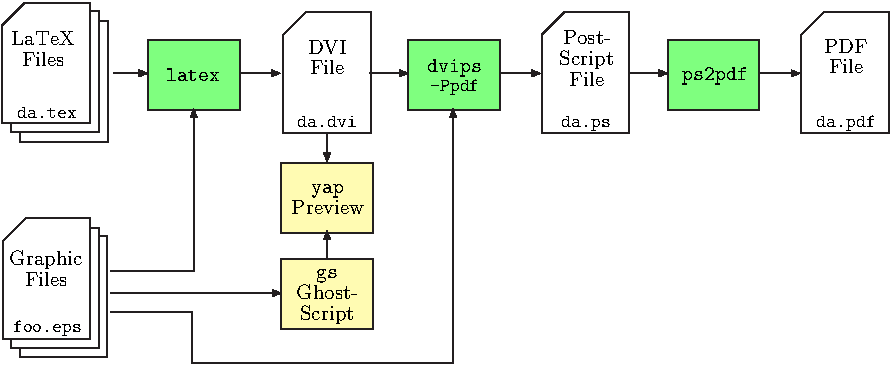
\includegraphics[width=1.0\textwidth]{workflow-cm}
\caption{Erzeugung von
PDF-Doku\-men\-ten im DVI-PS-Workflow. EPS-Grafiken werden erst bei der
Erzeugung der PS-Datei eingebunden. 
Anmerkung: Die abgebildete Vektorgrafik wurde mit \emph{Freehand} unter
Verwendung der \emph{BaKoMa} TrueType-Schriften erstellt %
(s.\ Abschn.\ \ref{sec:tex-schriften-in-grafiken}).}
\label{fig:latex-pdf-workflow}
\end{figure}

\end{comment}


\section{Drucken}

Vor dem Drucken der Arbeit empfiehlt es sich, einige Dinge zu beachten, um unnötigen Aufwand (und auch Kosten) zu vermeiden.

\subsection{Drucker und Papier}

Die Abschlussarbeit sollte in der Endfassung unbedingt auf einem
qualitativ hochwertigen Laserdrucker ausgedruckt werden, Ausdrucke
mit Tintenstrahldruckern sind \emph{nicht} ausreichend. Auch das
verwendete Papier sollte von guter Qualität (holzfrei) und
üblicher Stärke (mind.\ $80\; {\mathrm g} / {\mathrm m}^2$) sein.
Falls \emph{farbige} Seiten notwendig sind, sollte man diese einzeln%
\footnote{Tip: Mit \emph{Adobe Acrobat} lassen sich sehr einfach einzelne Seiten
des Dokuments für den Farbdruck auswählen und zusammenstellen.}
auf einem Farb-Laserdrucker ausdrucken und dem Dokument beifügen.

Übrigens sollten \emph{alle} abzugebenden Exemplare {\bf
gedruckt} (und nicht kopiert) werden! Die Kosten für den Druck
sind heute nicht höher als die für Kopien, der
Qualitätsunterschied ist jedoch -- \va\ bei Bildern und Grafiken
-- meist deutlich.


\subsection{Druckgröße}

Zunächst sollte sichergestellt werden, dass die in der fertigen PDF-Datei eingestellte
Papiergröße tatsächlich \textbf{A4} ist! Das geht \zB\ mit \emph{Adobe Acrobat}
oder \emph{SumatraPDF}
über \texttt{File} $\rightarrow$ \texttt{Properties},
wo die Papiergröße des Dokuments angezeigt wird:
\begin{center}
\textbf{Richtig:} A4 = $8{,}27 \times 11{,}69$ in \bzw\ $21{,}0 \times 29{,}7$ cm.
\end{center}
Falls das nicht stimmt, ist vermutlich irgendwo im Workflow versehentlich \textbf{Letter} 
als Papierformat eingestellt, %, häufig ist \emph{Adobe Distiller} "`schuld"'.


Ein häufiger und leicht zu übersehender Fehler beim Ausdrucken von
PDF-Dokumenten wird durch die versehentliche Einstellung der
Option "`Fit to page"' im Druckmenü verursacht, wobei die Seiten
meist zu klein ausgedruckt werden. Überprüfen Sie daher die Größe
des Ausdrucks anhand der eingestellten Zeilenlänge oder mithilfe
einer Messgrafik, wie am Ende dieses Dokuments gezeigt.
Sicherheitshalber sollte diese Messgrafik bis zur
Fertigstellung der Arbeit beibehalten und die entsprechende
Seite erst ganz am Schluss zu entfernt werden.
Wenn, wie häufig der Fall, einzelne Seiten getrennt in Farbe gedruckt 
werden, so sollten natürlich auch diese genau auf die Einhaltung der Druckgröße 
kontrolliert werden!




\section{Binden}

Die Endfassung der Abschlussarbeit%
\footnote{Für \textbf{Bachelorarbeiten} genügt, je nach Vorgaben des Studiengangs, meist eine einfache Bindung (Copyshop oder Bibliothek).}
ist in fest gebundener Form
einzureichen.%
\footnote{An der Fakultät Hagenberg ist bei Masterarbeiten zumindest eines der
Exemplare \emph{ungebunden} abzugeben -- dieses wird später von einem
Buchbinder in einheitlicher Form gebunden und verbleibt
danach in der Bibliothek. Datenträger sind bei diesem Exemplar lose 
und \emph{ohne} Aufkleber (jedoch beschriftet) beizulegen.}
Dabei ist eine Bindung zu
verwenden, die das Ausfallen von einzelnen Seiten nachhaltig
verhindert, \zB durch eine traditionelle Rückenbindung
(Buchbinder) oder durch handelsübliche Klammerungen aus Kunststoff
oder Metall. Eine einfache Leimbindung ohne Verstärkung ist
jedenfalls \emph{nicht} ausreichend.


Falls man -- was sehr zu empfehlen ist -- die Arbeit bei einem
professionellen Buchbinder durchführen lässt, sollte man auch auf
die Prägung am Buchrücken achten, die kaum zusätzliche Kosten
verursacht. Üblich ist dabei die Angabe des Familiennamens des
Autors und des Titels der Arbeit. Ist der Titel der Arbeit zu
lang, muss man notfalls eine gekürzte  Version angeben, wie \zB:
%
\begin{center}
\setlength{\fboxsep}{3mm}
\fbox{
\textsc{Schlaumeier}
\textperiodcentered\ \textsc{Part.\ Lösungen zur allg.\ Problematik}}
\end{center}
%



\section{Elektronische Datenträger (CD-R, DVD)}
Speziell bei Arbeiten im Bereich der Informationstechnik (aber
nicht nur dort) fallen fast immer Informationen an, wie Programme,
Daten, Grafiken, Kopien von Internetseiten \usw, die für eine
spätere Verwendung elektronisch verfügbar sein sollten.
Vernünftigerweise wird man diese Daten während der Arbeit bereits
gezielt sammeln und der fertigen Arbeit auf einer CD-ROM oder DVD
beilegen. Es ist außerdem sinnvoll -- schon allein aus Gründen der
elektronischen Archivierbarkeit -- die eigene Arbeit selbst als
PDF-Datei beizulegen.%
\footnote{Auch Bilder und Grafiken könnten in elektronischer Form nützlich
sein, die \latex- oder Word-Dateien sind hingegen überflüssig.}


Falls ein elektronischer Datenträger (CD-ROM oder DVD) beigelegt
wird, sollte auf folgende Dinge geachtet werden:
%
\begin{enumerate}
\item Jedem abzugebenden Exemplar muss eine identische Kopie des
Datenträgers beiliegen. %
\item Verwenden Sie qualitativ hochwertige Rohlinge und überprüfen
Sie nach der Fertigstellung die tatsächlich gespeicherten Inhalte
des Datenträgers! %
\item Der Datenträger sollte in eine im hinteren Umschlag
eingeklebte Hülle eingefügt sein und sollte so zu entnehmen sein,
dass die Hülle dabei \emph{nicht} zerstört wird (die
meisten Buchbinder haben geeignete Hüllen parat). %
\item Der Datenträger muss so beschriftet sein, dass er der
Abschlussarbeit eindeutig zuzuordnen ist, am Besten durch ein
gedrucktes Label%
\footnote{Nicht beim lose abgegebenen Bibliotheksexemplar --
dieses erhält ein standardisiertes Label durch die Bibliothek.} %
oder sonst durch \emph{saubere}
Beschriftung mit
der Hand und einem feinen, wasserfesten Stift. %
\item Nützlich ist auch ein (grobes) Verzeichnis der Inhalte des
Datenträgers (wie exemplarisch in Anhang \ref{app:cdrom}).
\end{enumerate}

%
% Einleitung: evtl. erklären was Begriffe bedeuten? so wie bei Paul Em?
%
% Wie wärs mit ease of use / Verwendung für andere developer? Erstellen von Präsentation evtl. als eigener Part?
%
%\chapter[Schlussbemerkungen]%
        {Schlussbemerkungen%
        \protect\footnote{Diese Anmerkung dient nur dazu, die (in seltenen Fällen sinnvolle)
				Verwendung von Fußnoten bei Überschriften zu demonstrieren.}}%
\label{cha:Schluss}

An dieser Stelle sollte eine Zusammenfassung der Abschlussarbeit
stehen, in der auch auf den Entstehungsprozess, persönliche
Erfahrungen, Probleme bei der Durchführung,
Verbesserungsmöglichkeiten, mögliche %
Erweiterungen \usw\ eingegangen werden kann. War das Thema richtig
gewählt, was wurde konkret erreicht, welche Punkte blieben offen
und wie könnte von hier aus weitergearbeitet werden?


\section{Lesen und lesen lassen}

Wenn die Arbeit fertig ist, sollten Sie diese zunächst selbst nochmals vollständig und sorgfältig durchlesen, auch wenn man vielleicht das mühsam entstandene Produkt längst nicht mehr sehen möchte. Zusätzlich ist sehr zu empfehlen, auch einer weiteren Person diese Arbeit anzutun -- man wird erstaunt sein, wie viele Fehler man selbst überlesen hat. 



\section{Checkliste}

Abschließend noch eine kurze Liste der wichtigsten Punkte, an denen erfahrungsgemäß die häufigsten Fehler auftreten (Tab.\ \ref{tab:checkliste}).


\begin{table}
\caption{Checkliste. Diese Punkte bilden auch die Grundlage der routine\-mäßigen Formbegutachtung in Hagenberg.}
\label{tab:checkliste}
\centering
\fbox{
\begin{minipage}{0.95\textwidth}
\medskip
\begin{itemize}
	\item[$\Box$] \textbf{Titelseite:} Länge des Titels (Zeilenumbrüche), Name, Studiengang, Datum.
	\item[$\Box$] \textbf{Erklärung:} vollständig Unterschrift.
	\item[$\Box$] \textbf{Inhaltsverzeichnis:} balancierte Struktur, Tiefe, Länge der Überschriften.
	\item[$\Box$] \textbf{Kurzfassung/Abstract:} präzise Zusammenfassung, passende Länge, gleiche Inhalte und Struktur.
	\item[$\Box$] \textbf{Überschriften:} Länge, Stil, Aussagekraft.
	\item[$\Box$] \textbf{Typographie:} sauberes Schriftbild, keine "`manuellen"' Abstände zwischen Absätzen oder Einrückungen, keine überlangen Zeilen, Hervorhebungen, Schriftgröße, Platzierung von Fußnoten.
	\item[$\Box$] \textbf{Interpunktion:} Binde- und Gedankenstriche richtig gesetzt, Abstände nach Punkten (\va\ nach Abkürzungen).
	\item[$\Box$] \textbf{Abbildungen:} Qualität der Grafiken und Bilder, Schriftgröße und -typ in Abbildungen, Platzierung von Abbildungen und Tabellen, Captions. Sind \emph{alle} Abbildungen (und Tabellen) im Text referenziert?
	\item[$\Box$] \textbf{Gleichungen/Formeln:} mathem.\ Elemente auch im Fließtext richtig gesetzt, explizite Gleichungen richtig verwendet, Verwendung von mathem.\ Symbolen.
	\item[$\Box$] \textbf{Quellenangaben:} Zitate richtig referenziert, Seiten- oder Kapitelangaben.
	\item[$\Box$] \textbf{Literaturverzeichnis:} mehrfach zitierte Quellen nur einmal angeführt, Art der Publikation muss in jedem Fall klar sein, konsistente Einträge, Online-Quellen (URLs) sauber angeführt.
	\item[$\Box$] \textbf{Sonstiges:} ungültige Querverweise (\textbf{??}), Anhang, Papiergröße der PDF-Datei 
	(A4 = $8.27 \times 11.69$ Zoll), Druckgröße und -qualität.
\end{itemize}
\medskip
\end{minipage}%
}
\end{table}



% Hier könnte man erwähnen dass das sharen mittels handy übers menü doch irgendwie besser wäre, aber den Nachteil hat dass man sich die app herunterladen muss.
% erwähnen: Könnte evtl. auch für remote presentationen verwendet werden!
% erwähnen: evtl. andere typen von Charts (Pie etc.) wie erwähnt in Electronic voting on the fly
% auszerdem: von power point exportieren wäre riesen Vorteil für Author!
% Wie wärs mit: Hinweis darauf, dass es wichtig ist die richtigen Mechanismen für die richtige Präsentation zu wählen um death by technology zu vermeiden (referenz zu \cite{Wacker:PresenterExperience}, dass failing technology reason #1 ist sich unwohl zu fühlen!). Mechanismen sollen nicht menschliche Kommunikation ersetzen sonder unterstützen und sind nicht immer nötig und mit Vorsicht zu genieszen
% Application for workshop environment (wie am Anfang besprochen! Großgruppe => Kleingruppe => Großgruppe)
% Sicherheitsconcerns nicht beachtet 
% Mehr tests benötigt, aber erste tests zeigen: Anfangsslide zum Austoben einbauen, App wird gut angenommen auch wenn Funktionen in Meetings mehr genutzt werden als in anderen Präsentationen
% Speichern der Resultate auf Implementierungsseite noch benötigt

%%%----------------------------------------------------------
%%%Anhang
\appendix
%\chapter{Technische Informationen}
\label{ch:TechnischeInfos}

\newcommand*{\checkbox}{{\fboxsep 1pt%
\framebox[1.30\height]{\vphantom{M}\checkmark}}}

\section{Aktuelle Dateiversionen}

\begin{center}
\begin{tabular}{|l|l|}
\hline
Datum & Datei \\
\hline\hline
\hgbthesisDate & \texttt{hgbthesis.cls} \\
\hline
\hgbDate       & \texttt{hgb.sty} \\
\hline
\end{tabular}
\end{center}




\section{Details zur aktuellen Version}


Das ist eine völlig überarbeitete Version der DA/BA-Vorlage, die
\mbox{UTF-8} kodierten Dateien vorsieht und ausschließlich im PDF-Modus arbeitet.
Der "`klassische"' DVI-PS-PDF-Modus wird somit nicht mehr unterstützt! 

\subsection{Allgemeine technische Voraussetzungen}

Eine aktuelle \latex-Installation mit
\begin{itemize}
	
		\item Texteditor für \mbox{UTF-8} kodierte (Unicode) Dateien,
		\item \texttt{biber}-Programm (BibTeX-Ersatz, Version $\geq 1.5$),
		\item \texttt{biblatex}-Paket (Version $\geq 2.5$, 2013/01/10),
		\item Latin Modern Schriften (Paket \texttt{lmodern}).%
			\footnote{\url{http://www.ctan.org/pkg/lm}, \url{http://www.tug.dk/FontCatalogue/lmodern}}
\end{itemize}


\subsection{Verwendung unter Windows}

Eine typische Installation unter Windows sieht folgendermaßen aus
(s.\ auch Abschnitt \ref{sec:Windows}):
%
\begin{enumerate}
\item \textbf{MikTeX 2.9}%
	\footnote{\url{http://www.miktex.org/} -- \textbf{Achtung:} 
	Generell wird die \textbf{Komplett\-installation} von MikTeX ("`Complete MiKTeX"') empfohlen, 
	da diese bereits alle notwendigen Zusatzpakete und Schriftdateien enthält! 
	Bei der Installation ist darauf zu achten, 
	dass die automatische Installation erforderlicher Packages 
	durch "`\emph{Install missing packages on-the-fly: = Yes}"' ermöglicht wird (NICHT "`\emph{Ask me first}"')!
	Außerdem ist zu empfehlen, unmittelbar nach der Installation von MikTeX mit dem Programm
	\texttt{MikTeX} $\to$ \texttt{Maintenance} $\to$ \texttt{Update} und \texttt{Package Manager} 
	ein Update der installierten Pakete durchzuführen.}
	(zurzeit am einfachsten die 32-Bit Version, da nur diese das Programm \texttt{biber.exe} 
	bereits enthält),
\item \textbf{TeXnicCenter 2.0}%
	\footnote{\url{http://www.texniccenter.org/}}
	(Editor-Umgebung, unterstützt UTF-8),
\item \textbf{SumatraPDF}%
	\footnote{\url{http://blog.kowalczyk.info/software/sumatrapdf/}} 
	(PDF-Viewer),
\end{enumerate}
%
Ein passendes TeXnicCenter-Profil für MikTeX, Biber und Sumatra ist in diesem Paket enhalten
(Datei \verb!_tc_output_profile_sumatra_utf8.tco!). Dieses sollte man zuerst
über \texttt{Build} $\to$ \texttt{Define Output Profiles} in TeXnicCenter importieren.
\textbf{Achtung}: Alle neu angelegten \texttt{.tex}-Dateien sollten in UTF-8 Kodierung gespeichert werden!




\subsection{Verwendung unter Mac~OS}


Diese Version sollte insbesondere mit \emph{MacTeX} problemlos laufen (s.\ auch Abschnitt \ref{sec:MacOs}):
\begin{enumerate}
\item 
	\emph{MacTex} (2012 oder höher).
\item 
	Die Zeichenkodierung des Editors sollte auf UTF-8 eingestellt sein.
\item 
	Als Engine (vergleichbar mit den Ausgabeprofilen in TeXnicCenter) sollte \emph{LaTeXMk} verwendet werden. 
	Dieses Perl-Skript erkennt automatisch, wie viele Aufrufe von \emph{pdfLaTeX} und \emph{Biber} nötig sind. 
	Die Ausgabeprofile \emph{LaTeX} oder \emph{pdfLaTeX} hingegen müssen mehrmals aufgerufen werden, 
	zudem werden hierbei auch die Literaturdaten nicht verarbeitet. Dazu müsste extra die \emph{Biber}-Engine 
	aufgerufen werden, 	die jedoch noch nicht in allen Editoren vorhanden ist.
\end{enumerate}


\begin{comment}
\subsection{Vorteile}
\begin{itemize}
\item PDF wird direkt erzeugt ohne DVI und PS; damit ist angeblich auch die "`Feintypographie"' besser.
\item Die Verwendung von \texttt{SumatraPDF} erlaubt funktionierende Forward- und Inverse-Suche, womit erstmals ein effektiver PDF-Workflow möglich ist.
\item Preview der vollständigen Manuskripts (inklusive Grafiken) ist in PDF viel schneller
als in DVI (mit YAP und Ghostscript für die Grafiken).
\item Grafiken können auch als PDF, PNG oder JPEG direkt eingebunden werden. Bestehende EPS-Grafiken werden automatisch in PDF konvertiert. 
\item Bei eingebundenen Rasterbildern werden (im Unterschied zu \texttt{ps2pdf} in der Default-Einstellung) keine zusätzlichen JPEG-Artefakte erzeugt. 
(Anmerkung: im TC-Ausgabeprofil für \texttt{ps2pdf} ist dafür jetzt die
Option \verb!-dPDFSETTINGS=/prepress! eingestellt -- \verb!=/printer! ist nicht ausreichend!)
\item Die Erzeugung von aktiven Verweisen mit \texttt{hyperref} funktioniert problemlos, mit allen Vorteilen (einschließlich der Zeilenumbrüche in URLs).
\item PDF-Metadaten (zur verbesserten Suche) werden direkt aus den Dokumentendaten durch LaTeX generiert.
\end{itemize}

\subsection{Weitere Neuerungen}
%
\begin{sloppypar}
\begin{itemize}
\item Verwendung des \texttt{epstopdf}-Pakets, wodurch vorhandene EPS-Grafiken (mit denen \texttt{pdflatex} nicht umgehen kann) automatisch in PDF-Dateien konvertiert werden, unter der Annahme, dass \texttt{epstopdf.exe} vorhanden ist. Das ist bei Rasterbildern allerdings nicht zu enpfehlen, weil mit \texttt{epstopdf} die Kompressionsqualität nicht gesteuert erden kann. In diesem Fall ist es besser, die EPS-Dateien (\zB\ mit PhotoShop) direkt in PDFs zu konvertieren oder (noch besser) die Original JPEG- oder PNG-Dateien zu verwenden.
%
\item Unter \texttt{pdflatex} können nun (mit \verb!\includegraphics{}!) neben PDFs auch Bilder im JPEG- oder PNG-Format direkt eingebunden werden. Alle Datei-Extensions der Grafikdateien wurden im Quelltext entfernt.
%
\item 
Verwendung des \textbf{SumatraPDF}-Viewers anstelle von Adobe Acrobat, da Acrobat das Überschreiben der Ausgabedatei blockiert (unter Windows) und forward/inverse Suche schlecht \bzw\ gar nicht unterstützt.
Anweisungen zur Einstellung findet man unter \url{http://www.hehn.biz/Mar/How_to_Sumatra.pdf} -- diese sind auch im beiliegenden TC-Aus\-gabe\-profil implementiert.
%
\item Verwendung des \texttt{pdfsync}-Pakets zur Unterstützung der inversen Suche aus PDF-Dateien.
%
\item Verwendung des \texttt{hyperref}-Pakets zur Aktivierung von Links (Web, Inhaltsverzeichnis, Querverweise, Literatur etc.). Erzeugt auch eine Navigation-Pane.
%
\item PDF-Metadaten werden automatisch aus den Dokumentendaten generiert (durch \texttt{hyperref} möglich).
%
\item Verwendung des \texttt{breakurl}-Pakets, mit dem Zeilenumbrüche trotz \texttt{hy\-per\-ref} auch bei DVI-PS-PDF-Generierung durchgeführt werden. Dadurch sind jetzt auch URLs in Captions und Fußnoten problemlos möglich und auch \verb!\urldef{}! ist nicht mehr erforderlich (entspr.\ Textpassagen in \ref{sec:QuellenangabenInCaptions} entfernen!). 
%
\item Alle bestehenden EPS-Dateien mit Rasterbildern wurden auf Binärkodierung umgestellt, da dies mit der aktuellen MikTeX-Version keine Probleme mehr verursacht. Zusätzlich wurden PNG-Versionen für \texttt{pdflatex} angelegt, sodass keine automatische Umwandlung mit \texttt{epstopdf} erfolgt.
%
\item
Das lästige Problem des übermäßigen vertikalen Abstände in LaTeX-Aufzählungslisten wurde mit dem \texttt{enumitem}-Paket behoben. Alle \verb!\itemsep0pt! Anweisungen im Text wurden entfernt.
%
\item Einbindung des \texttt{cite}-Pakets mit \texttt{noadjust}-Option, womit kein zusätzliches Spacing erzeugt wird.
\end{itemize}
\end{sloppypar}
\end{comment}


\begin{comment}
\section{Einstellungen unter Windows} 
\label{sec:EinstellungAusgabeprofile}

Die folgenden Angaben beziehen sich auf eine bewährte Arbeitsumgebung unter Windows (XP, Win7) mit MikTeX, Sumatra-PDF und TeXnicCenter, mit folgenden Installationspfaden:
%
\begin{quote}
\verb!C:\Program Files (x86)\MiKTeX 2.9\! \\
\verb!C:\Program Files (x86)\SumatraPDF\! \\
\verb!C:\Program Files (x86)\TeXnicCenter\! 
\end{quote}
%
Unter Windows XP liegen die Programme in \verb!C:\Program Files\!.
Falls neuere Versionen dieser Komponenten installiert sind, müssen natürlich die nachfolgend angegebenen Pfade entsprechend modifiziert werden.

\begin{quote}
\textbf{Achtung:} Für MikTeX immer die \textbf{komplette Version} installieren! Das entsprechende Installationsverzeichnis hat aktuell einen Umfang von ca.\ 1.2 GB und enthält etwa 53.200 Dateien 
(typischerweise in \nolinkurl{C:\\Program Files (x86)\\MiKTeX...}).
\end{quote}
\end{comment}

\begin{comment}
\subsection{TeXnicCenter-Ausgabeprofile}
\label{sec:TeXnicCenterUndMikTeX}

TeXnicCenter definiert den Verarbeitungsablauf des LaTeX-Dokuments anhand von Ausgabeprofilen, wobei die oben genannten Komponenten als externe Programme mit entsprechenden Argumenten aufgerufen werden.
Die Einstellung der Ausgabeprofile erfolgt in TeXnicCenter über das Menü
\textsf{Ausgabe}$\rightarrow$\textsf{Ausgabeprofile definieren...} (Abb.\ \ref{fig:techniccenter-profile-latex}). 
Die Profile werden (abhängig von der installierten Software) üblicherweise beim ersten Start von TeXnicCenter durch den zugehörigen "`Wizard"' voreingestellt. 

\begin{figure}
\centering\small
\setlength{\tabcolsep}{0pt}%
\begin{tabular}{c@{~}c}
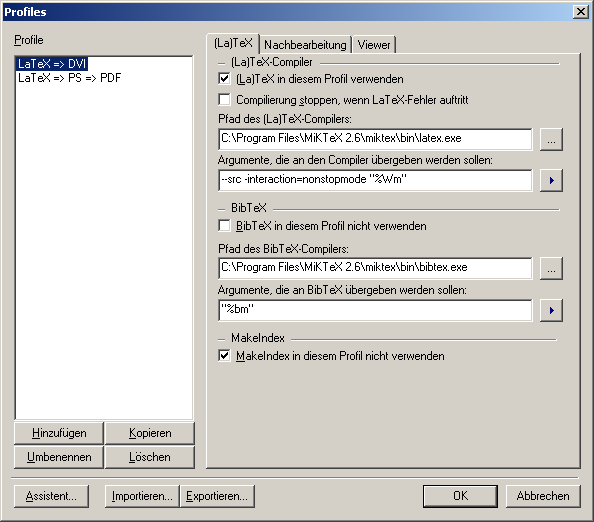
\includegraphics[width=0.49\textwidth]{techniccenter-profile-dvi-26} &
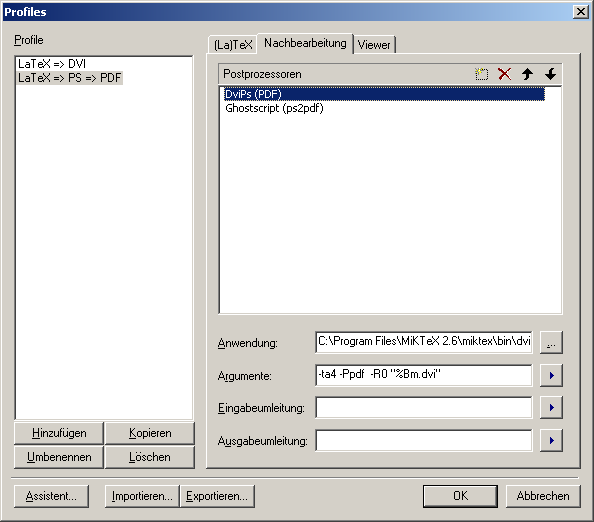
\includegraphics[width=0.49\textwidth]{techniccenter-profile-dvips-26} \\[4pt]
(a) & (b)
\end{tabular}
\caption{Spezifikation der Ausgabeprofile in TeXnicCenter.}
\label{fig:techniccenter-profile-latex}
\end{figure}

In der Datei \verb!tc_output_profiles_sumatra.tco! sind  folgende beiden "`maßgeschneiderten"' Ausgabeprofile für TexNicCenter angelegt (Import über \textsf{Build} $\rightarrow$ \textsf{Define Output Profiles ...}):
\begin{itemize}
	\item \verb!LaTeX => PDF (Sumatra)! -- Standard, direkte Erzeugung von PDF,
	\item \verb!LaTeX => PS => PDF (Sumatra)! -- PDF "`klassisch"' via DVI und PS.
\end{itemize}

\subsubsection{Profil "`\texttt{LaTeX => PDF (Sumatra)}"'}

Das ist das mit diesem Setup normalerweise verwendete Standardprofil.

\paragraph{(La)Tex:}
\begin{itemize}
  \item Path to the (La)TeX compiler: \\
        \begin{small} \verb!C:\Program Files (x86)\MiKTeX 2.9\miktex\bin\pdflatex.exe!\end{small}
  \item Command line arguments to pass to the compiler:\\
\begin{small}
   \verb!-synctex=-1 -interaction=nonstopmode "%pm"!
\end{small}
\end{itemize}

\paragraph{Postprocessor:} 
leer, kein Postprocessor notwendig.

\paragraph{Viewer:}
\begin{itemize}
\item Path of executable: \\
\begin{small}
    \verb!C:\Program Files (x86)\SumatraPDF\SumatraPDF.exe ! \\ 
    \verb!-inverse-search "\"C:\Program Files\TeXnicCenter\TEXCNTR.EXE\" !\\
    \verb!/ddecmd \"[goto('%f','%l')]\""!
\end{small}
%
\item View project's output: \\
\begin{small}
    \checkbox\ Command line argument \\\
    Command: \verb!"%bm.pdf"!
\end{small}
%
\item Forward search:\\
\begin{small}
    \checkbox\ DDE command \\\
    Command: \verb![ForwardSearch("%bm.pdf","%Wc",%l,0)]! \\
    Server: \verb!SUMATRA! \\
    Topic: \verb!Control!
\end{small}
\item Close document before running (La)TeX:\\
\begin{small}
    \checkbox\ Do not close
\end{small}
\end{itemize}


\subsubsection{Profil "`\texttt{LaTeX => PS => PDF (Sumatra)}"'}

Profil ausschließlich für den DVI-PS-Workflow (über DVI und PostScript).

\paragraph{(La)Tex:}
\begin{itemize}
  \item Path to the (La)TeX compiler: \\
        \begin{small} \verb!C:\Program Files (x86)\MiKTeX 2.9\miktex\bin\latex.exe!\end{small}
  \item Command line arguments to pass to the compiler:\\
\begin{small}
   \verb!-synctex=-1 -interaction=nonstopmode "%pm"!
\end{small}
\end{itemize}

\paragraph{Postprocessor:}
\begin{itemize}
  \item DviPS (PDF): \\
        \begin{small} 
        Executable: \verb!C:\Program Files (x86)\MiKTeX 2.9\miktex\bin\dvips.exe! \\
        Arguments: \verb!-ta4 -P pdf -R0 "%Bm.dvi"!
        \end{small}
  \item Ghostscript (ps2pdf):\\
  		\begin{small} 
        Executable: \verb!C:\Program Files (x86)\gs\gs9.04\bin\gswin32c.exe! \\
        Arguments: \verb!-q -dPDFSETTINGS=/prepress -sPAPERSIZE=a4 -dSAFER! \\
         \verb!-dBATCH -dNOPAUSE -sDEVICE=pdfwrite -sOutputFile="%bm.pdf"! \\
         \verb!-c save pop -f "%bm.ps"!
      \end{small}
\end{itemize}

\paragraph{Viewer:}
wie in Profil A. (\texttt{LaTeX => PDF (Sumatra)}).

\section{Tipps und offene Probleme:}

\begin{itemize}
\item \texttt{psfrag} funktioniert nicht mit \texttt{pdflatex} und es gibt auch leider keine Ersatzlösung. 
Wenn man \texttt{psfrag} braucht, dann muss man weiterhin über PostScript 
(\verb!LaTeX => PS => PDF!) arbeiten (was allerdings nunmehr auch mit \texttt{hyperref} kein Problem mehr ist).
%
\item Bei Verwendung des TexWorks-Editors (wird mit MikTeX ausgeliefert) sollte man die Standard-Zeichenkodierung von \emph{Unicode} (utf8) auf \emph{Latin-1} (ISO 8859-1) umstellen.
%
\item Adobe Illustrator kann beim Speichern als PDF die Bounding Box nicht setzen. 
Eine Möglichkeit ist, die Grafik zuerst als EPS zu exportieren und dann mit Acrobat in ein PDF zu konvertieren. 
%
\end{itemize}
\end{comment}



\begin{comment}
\section{Einstellungen für YAP (DVI-Viewer) im DVI-PS-Workflow}
\label{sec:YapEinstellung}

Im Standard-DVI-Viewer YAP lässt sich durch Mausklick auf das DVI-Dokument sehr leicht die zugehörige Stelle im Quelltext finden. Im Normalfall öffnet dann TeXnicCenter das zugehörige \latex-Dokument automatisch an der richtigen Stelle.
Das zugehörige "`Inverse DVI Search"' Kommando sollte sich bereits bei der Installation richtig einstellen.

Falls dies \emph{nicht} funktioniert, kann man in YAP diese Einstellung auch manuell über das Menü \textsf{View}\thinspace$\rightarrow$\thinspace\textsf{Options...} vornehmen, wie in Abb.\ \ref{fig:yap-inverse-search} gezeigt.
In diesem Fall lautet die vollständige Anweisung in "`Command Line"' folgendermaßen:
\begin{center}\footnotesize
\verb!"C:\Program Files (x86)\TeXnicCenter\TEXCNTR.EXE" /ddecmd "[goto('%f', '%l')]"!
\end{center}


\begin{figure}
\centering\small
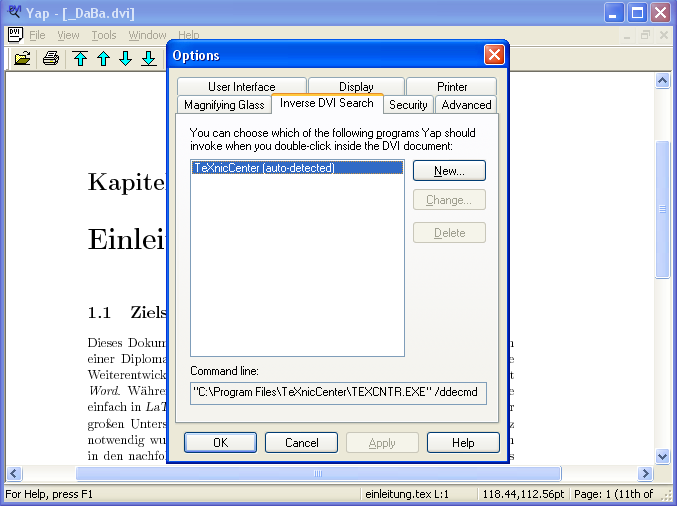
\includegraphics[width=1.0\textwidth]{yap-inverse-search-settings}
\caption{"`Inverse DVI Search"' Einstellung in YAP (über das Menü \textsf{View}\thinspace$\rightarrow$\thinspace\textsf{Options...}).}
\label{fig:yap-inverse-search}
\end{figure}

Latex
C:\Program Files\MiKTeX 2.6\miktex\bin\latex.exe
--src -interaction=nonstopmode "%Wm"

Bibtex
C:\Program Files\MiKTeX 2.6\miktex\bin\bibtex.exe
"%bm"

---

DviPs (PDF)
C:\Program Files\MiKTeX 2.6\miktex\bin\dvips.exe
-ta4 -Ppdf  -R0 "%Bm.dvi"

Ghostscript (ps2pdf)
C:\Program Files\gs\gs8.61\bin\gswin32c.exe
-sPAPERSIZE=a4 -dSAFER -dBATCH -dNOPAUSE -sDEVICE=pdfwrite -dPDFSETTINGS=/prepress -sOutputFile="%bm.pdf" -c save pop -f "%bm.ps"


YAP 
Options -> Inverse Search
"C:\Program Files\TeXnicCenter\TEXCNTR.EXE" /ddecmd "[goto('%f', '%l')]"

\end{comment}

	% Technische Ergänzungen
%
%\chapter{Inhalt der CD-ROM/DVD}
\label{app:cdrom}

\paragraph{Format:} 
		CD-ROM, Single Layer, ISO9660-Format%
\footnote{Verwenden Sie möglichst ein Standardformat, bei DVDs natürlich
eine entsprechende andere Spezifikation.}


\section{PDF-Dateien}
\begin{FileList}{/}
%\fitem{_DaBa.dvi} Gesamtdokument (DVI-File, ohne Grafiken)
\fitem{_DaBa.pdf} Master- oder Bachelorarbeit mit Instruktionen (Gesamtdokument)
\fitem{_PrBericht.pdf} Praktikumsbericht (verkürzte Version der Bachelorarbeit) %
\end{FileList}


\section{\latex-Dateien}

\textbf{Achtung:} Die folgende Auflistung soll nur den Gebrauch dieser Vorlage erleichtern. Es ist bei einer Master- oder Bachelorarbeit \ia\ \emph{nicht} notwendig, die zugehörigen \latex-Dateien aufzulisten (wohl aber projektbezogene Dateien, Ergebnisse, Bilder, Kopien von Online-Literatur etc.)!

\begin{FileList}{/}
\fitem{_DaBa.tex} Master-/Bachelorarbeit (Hauptdokument) %
\fitem{_PrBericht.tex} Praktikumsbericht (verkürzte Version der Bachelorarbeit) %
\fitem{vorwort.tex} Vorwort %
\fitem{kurzfassung.tex} Kurzfassung %
\fitem{abstract.tex} Abstract %
\fitem{einleitung.tex} Kapitel 1 %
\fitem{diplomschrift.tex} Kapitel 2 %
\fitem{latex.tex} Kapitel 3
\fitem{abbildungen.tex} Kapitel 4 %
\fitem{formeln.tex} Kapitel 5 %
\fitem{literatur.tex} Kapitel 6 %
\fitem{drucken.tex} Kapitel 7 %
\fitem{word.tex} Kapitel 8 %
\fitem{schluss.tex} Kapitel 9 %
\fitem{anhang_a.tex} Anhang A (Source Code) %
\fitem{anhang_b.tex} Anhang B (Inhalt CD-ROM) %
\fitem{anhang_c.tex} Anhang C (Liste der Änderungen) %
\fitem{anhang_d.tex} Anhang D (LaTeX-Quellcode) %
\fitem{messbox.tex} Messbox zur Druckkontrolle %
\fitem{literatur.bib} Literatur-Datenbank (BibTeX-File)
\end{FileList}

\section{Style/Class-Dateien}

\begin{FileList}{/}
\fitem{hgbthesis.cls} LaTeX Class-Datei für Master- und Bachelorarbeiten
\fitem{hgbtermreport.cls} LaTeX Class-Datei für Semesterberichte
\fitem{hgb.sty} LaTeX Style-Datei für alle Hagenberg-Dokumente
\end{FileList}


\section{Sonstiges}

\begin{FileList}{/images}
\fitem{*.ai} Original Adobe Illustrator-Dateien %
\fitem{*.fh11} Original Macromedia Freehand-Dateien %
\fitem{*.jpg, *.png} Original Rasterbilder %
%\fitem{*.eps} Bilder und Grafiken im EPS-Format%
%\fitem{fonts-bakoma/} BaKoMa TrueType Fonts %
\end{FileList}
	% Inhalt der CD-ROM/DVD
%
%\chapter{Chronologische Liste der Änderungen}


\begin{sloppypar}
\begin{description}
%
\item[2002/01/07]
\verb!\newfloat{program}! repariert (auch ohne Chapter). Dank an Werner Bailer!
%
\item[2002/03/06]
Copyright-Notice an internat.\ Standard angepasst. Dank an Karin Kosina!
%
\item[2002/07/28]
"`Studiengang"' $\rightarrow$ "`Diplomstudiengang"'
%
\item[2003/08/24]
Neues Macro: \verb!\Messbox{breite}{hoehe}! -- zur Kontrolle der 
Druckgröße ohne PS-Datei. Erweiterungen für Bakkalaureatsarbeiten
%
\item[2005/04/09]
Diverse Korrekturen: Captions von Tabellen nach oben gesetzt. 
\texttt{caption} auf neue Versionen adaptiert.
\texttt{subfigure} wird nicht mehr verwendet
%
\item[2006/01/20]
Adaptiert zur Verwendung als Praktikumsbericht 
(2.\ Bakk.-Arbeit)
%
\item[2006/03/24]
Fehler in \verb!\erklaerung! beseitigt (Dank an David Schwingenschlögl)
%
\item[2006/04/06]
Verwendung von T1-Fontencoding zur besseren Silbentrennung bei 
Umlauten etc.
%
\item[2006/06/21]
Neu: Bachelorstudiengang / Masterstudiengang.
Literaturverweise auf Bakk-Arbeiten.
\texttt{upquote.sty} eliminiert (Problem mit TS1-Kodierung).
Verwende Komma (statt Punkt) als Trennzeichen in Dezimalzahlen.
%
\item[2006/09/14]
Anmerkungen zum Thema Plagiarismus.
%
\item[2007/07/16]
Ergänzungen für Code-Listings (listings) und Algorithmen 
(\texttt{algorithmicx}).
BiBTeX-Datei aufgeräumt, Verwendung der Literaturformate 
verbessert.
Komma (statt Punkt) als Trennzeichen in Dezimalzahlen wieder 
entfernt.
Verwendung der \texttt{ae}-Fonts eliminiert (\texttt{cm-super} Fonts müssen 
installiert sein, ab MikTeX 2.5). 
Beispiel für Ersetzung in EPS-Dateien mit \texttt{psfrag}.
%
\item[2007/10/04]
Version 5.90: Das Laden der Pakete \verb!inputenc! (Option \texttt{latin}) und 
\verb!graphicx! (Option \texttt{dvips})
aus der Hauptdatei in die \texttt{sty}-Datei übertragen; \texttt{upquote} funktioniert nun.
Paket \texttt{eurosym} ergänzt für Euro-Symbol (Anregung von Andreas 
Doubrava).
Problem mit \texttt{color}-package repariert (gerasterter PDF-Ausdruck).
Hinweise bzgl.\ Literatur ergänzt (\texttt{month}, \texttt{edition}),
BibTeX-Datei gesäubert.
Hinweis zum Einfügen von vertikalem Abstand zwischen Absätzen.
Mathematik aufgeräumt, Verwendung von \texttt{amsmath}, 
Fallunterscheidungen.
Diverse Änderungen bei Tabellen und Programmkode.
Beispiele für BibTeX-Angaben von Spezialquellen: Audio-CDs, 
Videos, Filme. Einbinden von Dateien mit \verb!\include{..}!
Neue Datei: \verb!_SimpleReport.tex! für kurze Reports (Projekte etc.).
%
\item[2007/11/11]
Version 5.91: Hinweise zur Einstellung der Output-Profile in
TexNicCenter, Inverse Search Einstellung in YAP im Anhang.
%
\item[2008/04/01]
Version 6.00beta -- kompletter Umbau!
Auslagerung der Doku\-menten-relevanten Teile in eine eigene 
\emph{class}-Datei (\texttt{hgbthesis.cls}) mit Optionen.
Die neue Style-Datei \texttt{hgb.sty} ist nun unabhängig vom 
Dokumententyp und nicht mehr kompatibel mit älteren Versionen!
Die Liste der Änderungen ist jetzt in der Datei \verb!_ChangeLog.tex!
(DIESE Datei) und diese wird im Anhang eingebunden.
Heading-Style auf Sans Serif geändert (ohne grausliche "`Caps"').
%
\item[2008/05/22]
Neue Vorlage für Technical Reports (Klasse \texttt{hgbreport.cls}).
Spracheinstellung nunmehr mit \texttt{babel}-Paket, Hauptsprache
des Dokuments kann als Option der Klasse angegeben werden.
Sprachumschaltung innerhalb des Dokuments funktioniert nun
richtig. Mit der Sprachoption \texttt{german} wird automatisch die neue deutsche 
Orthographie (\texttt{ngerman}) verwendet.
\texttt{babelbib} wird zur Formatierung des Literaturverzeichnisses
verwendet (neue BibTeX-Style-Optionen!).
Header werden nunmehr mit \texttt{fancyhdr}-Paket erzeugt.
Versionsnummerierung von \texttt{.cls} und \texttt{.sty} Files wird beendet 
(ab jetzt gilt: \emph{Datum} = \emph{Version}). 
%
\item[2008/06/10]
Neues Listing-Environment \texttt{PhpCode}; bei allen Listing-Eviron\-ments ist nun 
\texttt{mathescape=false} (kein Math-Mode nach \verb!$!). 
Bug bei Sprachumschaltung auf \texttt{ngerman} beseitigt.
%
\item[2008/08/15]
Diverse Kleinigkeiten in Literaturangaben überarbeitet (Dank an Norbert Wenzel), Spracheinstellung vereinheitlicht, Umlaute in \texttt{.bib}-Datei ersetzt.
%
\item[2008/10/15] 
Zusätzliche Hinweise zur MikTeX-Installation (Windows) sowie LaTeX unter Mac OS~X und Linux.
Liste der Abkürzungen ergänzt.%
\item[2008/11/15] 
Diverse Schreibfehler korrigiert (Dank an Silvia Fuchshuber). Hinweis auf 
\texttt{sloppypar}-Umgebung.
%
\item[2008/12/09] 
BibTeX-Tools: neuer Hinweis auf JabRef ergänzt, BibEdit entfernt (ist nicht mehr auffindbar).
%
\item[2009/02/09]
\texttt{hgb.sty}: Option "`\texttt{spaces}"' zu \texttt{url}-Package ergänzt (ermöglicht gezielten Zeilenumbruch in URLs). 
Im allgemeinen Setup für \texttt{listings}: \texttt{keepspaces=true};
Obsoletes Environment \texttt{sourcecode} deaktiviert.
Escape-Mode für \texttt{LaTeXCode}-Umgebung geändert.
\verb!_DaBa.tex!: Hinweis auf die Verwendung von \verb!\urldef! für die Angabe von URLs in Captions. \texttt{diplom} (statt \texttt{master}) als Standard-Dokumententyp in \verb!_DaBa.tex! ("`Diplomarbeit"'). Neuer Abschnitt zum Umgang mit ``Quellenangaben in Captions''.
\texttt{literatur.bib}: alle URLs (bisher in \texttt{note}-Einträgen) auf \verb!url={..}! geändert.
%
\item[2009/04/14]
Hinweis zum Einfügen einfacher Anführungszeichen ergänzt.
%
\item[2009/07/18]
Literaturangaben korrigiert und ergänzt.
%
\item[2009/11/27]
Experimentelle Version: Massive Änderungen, Umstieg auf \texttt{pdflatex}.
%
\item[2010/06/15]
Erstes Release der neuen Version mit \texttt{pdflatex}.
\item[2010/06/23]
Konflikt zwischen \texttt{pdfsync}-Package und \texttt{array}-Package (wird relativ häufig benutzt) durch \verb!\RequirePackage[novbox]{pdfsync}! behoben.
Seitenunterkante durch \verb!\flushbottom! fixiert,
variablen Absatzzwischenraum reduziert.
\item[2010/07/27]
Sprache der Erklärungsseite auf "`\texttt{german}"' fixiert (auch wenn die Hauptsprache des Dokuments  Englisch ist). %Datumsproblem - Hinweis von Philipp Winter
\item[2010/12/03]
Anmerkungen und Beispiele zum Zitieren von Gesetzestexten und Videos (Zeitangabe) ergänzt.
Hinweis auf \verb!\nolinkurl{..}! zur Angabe von Dateinamen.
\item[2011/01/29]
Einbau der Creative Commons Lizenz und entsprechender Hinweis in 
Abschnitt \ref{sec:HagenbergEinstellungen}. Neue Makros
\verb!\strictlicense!,
\verb!\cclicense! und
\verb!\license{...}!.
BibTeX-Einträge für Audio-CDs und Filme korrigiert, Beispiel für Online-Video ergänzt.
\item[2011/02/01]
Neues Makro \verb!\betreuerin{..}! zur Angabe einer (weiblichen) Betreuerin. 
%
\item[2011/06/26]
Umstellung der gesamten Literaturverwaltung auf \texttt{biblatex} mit dem Ziel, 
getrennte Abschnitte für verschiedene Kategorien von Einträgen im Quellenverzeichnis
zu ermöglichen. Die Wahl fiel auf \texttt{biblatex} (es gäbe andere Optionen), weil
damit BibTeX weiterhin nur einmal aufgerufen werden muss (und nicht für
mehrere Dateien). Damit verbunden sind allerdings massive Änderungen bei der
Syntax der BibTeX-Felder und es gibt auch mehrere neue Felder.
Aktuell sind 3 Kategorien von Quellen vorgesehen, entsprechende Änderungen in 
\nolinkurl{hgbthesis.cls}. Der klassische BibTeX-Workflow wird aktuell nicht
mehr unterstützt, die Möglichkeit einer künftigen Dok-Option ist aber 
vorgesehen. Das Literatur-Kapitel ist komplett überarbeitet, die .bib-Datei
wurde ausgemistet. Neu ist die Empfehlung zur Aufnahme von Bildquellen
in das Quellenverzeichnis, womit lange URLs in Captions (dort sind keine
Fußnoten möglich) nicht mehr notwendig sind. 
"`Persönliche Kommunikation"' als Literaturquelle entfernt (den Inhalt
von Interviews sollte man direkt im Anhang wiedergeben).
Das verwendete Bildmaterial wurde
erneuert, aktuell werden nur mehr Public Domain Bilder verwendet. 
Das Kapitel "`Hinweise für Word-Benutzer"' wurde endgültig entfernt.
\verb!\flushbottom! wieder auf \verb!\raggedbottom! geändert, um übermäßige 
Abstände zwischen Absätzen zu vermeiden.
%
\item[2012/05/10]
Hinweis auf die in Österreich bislang nicht zulässige Verwendung von "`Masterarbeit"'
entfernt, \texttt{master} ist nunmehr die Default-Dokumentenoption.
Anmerkungen zu lästigen \texttt{biblatex}-Warnungen ergänzt.
Angaben für Windows-Programmpfade auf Win7 angepasst, 
MikTeX 2.9 als Minimalerfordernis.\newline
Überflüssige Makros \verb!\damonat! und \verb!\dajahr! endgültig entfernt, statt
\verb!\abgabemonat! und \verb!\abgabejahr! ist nun das neue Makro
\verb!\abgabedatum{yyyy}{mm}{dd}! vorgesehen (unter Verwendung von internen Zählern).
Zur Formatierung von Datumsangaben wir das \texttt{datetime}-Paket verwendet.
\newline
Neue Fassung der eidesstattlichen Erklärung (inkl.\ englischer Version).\newline
PDF-Suche auf \texttt{synctex} umgestellt (\texttt{pdfsync}-Paket ist veraltet und
wird nun nicht mehr verwendet).
\newline
Die älteren Dateiversionen von \texttt{algorithmicx.sty} und \texttt{alg\-pseudo\-code.sty}
(bisher explizit beigefügt) wurden weggelassen.
\newline
Hinweis auf die \emph{Latin Modern Roman} OTF-Schriften ergänzt.
%
\item[2012/07/21]
Quellenverzeichnis: sprachabhängige Einstellung der Überschriften eingerichtet.
Titel des Quellenverzeichnisses auf "`Quellenverzeichnis"' (DE) \bzw\ "`References"' (EN) 
fixiert. Makro \verb!\MakeBibliography! hat damit keinen erforderlichen Parameter mehr.
%
\item[2012/09/17]
Wegen Änderungen im \texttt{biblatex}-package (Version 1.7, 2011/11/13) die Verwendung von
BibTeX als backend eingestellt (\texttt{backend=bibtex8}).
%
\item[2012/10/13]
Option \texttt{lowtilde} beim URL-package eingestellt (erzeugt \url{~} statt \verb!~!).
%
\item[2012/12/01]
In Abschnitt \ref{sec:FormatierungVonProgrammcode} zusätzliche Code-Umgebungen ergänzt:
\texttt{JsCode},
\texttt{PhpCode},
\texttt{HtmlCode},
\texttt{CssCode},
\texttt{XmlCode}.
%
\item[2012/12/08]
Die Code-Umgebungen in Abschn.\ \ref{sec:FormatierungVonProgrammcode} ergänzt und 
zur Verwendung von optionalen Argumenten erweitert (Hinweise in Abschnitt 
\ref{sec:FormatierungVonProgrammcode} auf die Argumente
\texttt{firstnumber=last} und \texttt{numbers=none}).
Quellenverzeichnis: den Eintragstyp \texttt{@software} für Games empfohlen und im Verzeichnis
der Kategorie \emph{avmedia} zugeordnet (Tab.~\ref{tab:BibKategorien} ergänzt). 
Game-Beispiel (von Manuel Wieser) und zusätzliche Tabelle \ref{tab:QuellenUndEintragstypen}
zur besseren Übersicht eingefügt.
%
\item[2013/05/17]
Wichtigste Änderung ist die vollständige Umstellung auf \textbf{UTF-8} unter Beibehaltung des 
\texttt{pdflatex}-Workflows. 
Damit sind zahlreiche weitere Modifikationen verbunden:
\newline
Alle Dateien (auch \texttt{.cls}, \texttt{.sty} und \texttt{.bib}) wurden auf UTF-8 konvertiert.
Damit sollte es auch keine Probleme mehr mit Umlauten und Sonderzeichen unter MacOS geben.
\newline
Die verwendete Standard-Schriftfamilie ist nun "`Latin Modern"' (\texttt{lmodern}). 
Sie ersetzt die "`CM-Super"' Schriften, mit denen es immer wieder Installationsprobleme gab.
Weiters wird jetzt das \texttt{cmap}-Paket zur besseren Such- und Kopierbarkeit von PDFs verwendet.
\newline
Das \texttt{listings}-Paket wurde durch \texttt{listingsutf8} ersetzt und für Umlaute im Quellcode adaptiert.
Eventuell sind weitere Adaptierungen notwendig.
\newline
\texttt{biber} (min.\ Version 1.5!) wird nun anstatt \texttt{bibtex} (unterstützt keine UTF-8 Dateien) verwendet,
zusammen mit \texttt{biblatex} (Version 2.5).
Die Anweisung \verb!\bibliography! wird (wieder) verwendet, allerdings nun in der Präambel,
um die \texttt{.bib}-Datei im Fileverzeichnis anzuzeigen.
\newline
Das Makro \verb!\C! (für die Menge der komplexen Zahlen \Cpx) musste wegen Problemen in der T1-Kodierung
ersetzt werden und heißt nun \verb!\Cpx!. Die Makros 
\verb!\R!, \verb!\Z!, \verb!\N!, \verb!\Q! und \verb!\Cpx! können nun auch außerhalb des Mathematik-Modus verwendet werden.
\newline
Der DVI-PS-PDF Workflow wird ab dieser Version überhaupt nicht mehr unterstützt. 
Damit ist auch das \texttt{psfrag}-Paket nicht mehr verwendbar. Entspechende Hinweise 
wurden aus dem Text entfernt.
\newline
\texttt{hyperref} wurde auf UTF-8 umgestellt.
Die grässlichen Standard-Rahmen und Farben der automatischen \texttt{hyperref}-Links wurden entfernt \bzw\ durch 
dezentere Farben ersetzt. Dadurch wird auch die Screen-Version der PDFs wieder lesbar.
\newline
Im Quellenverzeichnis wurde versuchsweise die \texttt{backref}-Option aktiviert. 
Damit werden bei allen Einträgen auch die zugehörigen Zitierstellen angegeben
(erscheint durchaus sinnvoll).
\newline
Die bisherigen Korrekturen zur \texttt{biblatex}-Formatierung wurden entfernt, 
alles arbeitet nun mit Standard-Einstellungen. Die ursächlichen Probleme in \texttt{biblatex}
scheinen in der aktuellen Version behoben zu sein.
\newline
Das Output-Profil für TeXnicCenter wurde für den neuen Workflow mit \texttt{biber} adaptiert und liegt nun in
\nolinkurl{_tc_output_profile_sumatra_utf8.tco}.
\newline
Das Windows-Script \verb!_clean.bat! wurde entfernt, da TeXnicCenter nun ein eigenes "`Clean Project"'-Kommando aufweist (in "`Build"').
\newline
Allgemeine Einstellungen zu \emph{headings} und \emph{biblatex} wurden aus der Datei \texttt{hgbthesis.cls} entfernt und in 
\texttt{hgbheadings.sty} \bzw\ \texttt{hgbbib.sty} verlagert. Diese können nun unabhängig verwendet werden (s.\ Beispiel in 
\texttt{\_TermReport.tex}).
\newline
Die Klassen-Datei \texttt{hgbtermreport.cls} wurde eliminiert, das Dokument \texttt{\_TermReport.tex} basiert nunmehr
auf der generischen LaTeX-Klasse \texttt{report}  und verwendet keine eigene \texttt{.cls} Datei mehr.
%
\item[2014/11/05]
Neu: Logo auf der Frontseite bei allen Dokumententypen. Dazu gibt es ein neues Kommando
\verb!\logofile{pic}!, wobei \verb!pic! der Name eine PDF-Datei im
Verzeichnis \verb!images/! ist. Falls \emph{kein} Logo erwünscht ist, 
kann man die Zeile einfach weglassen oder durch \verb!\logofile{}! ersetzen.
\newline
\texttt{hyperref}-Einstellungen: Einfärbung der Links wieder entfernt (\texttt{colorlinks = false}), weil beim Druck
nicht abschaltbar. Stattdessen einheitliche (dezente) Rahmen für alle Linkarten.
Zahlreiche Tippfehler eliminiert (Dank an Daniel Karzel).
\newline
Wegen eines Bugs in \texttt{biblatex 1.9} wurden die expliziten Abteilungen (\verb!\-!) in \texttt{literatur.bib}
vorübergehend entfernt (mit entsprechenden Folgen im Ergebnis). Der Bug soll in \texttt{biblatex 2.0} (derzeit noch
nicht verfügbar) behoben sein.
\newline
Package \texttt{color} auf \texttt{xcolor} geändert. In \texttt{hgb.sty} neues "`Convenience-Makro"' \verb!\etc! ergänzt.
Output-Profil für TeXnicCenter/SumatraPDF (Windows) repariert, forward/inverse Search funktioniert nun
(Datei \verb!_tc_output_profile_sumatra_utf8.tco!).
%
\item[2015/04/28]
Paket \texttt{subdepth} (zur verbesserten Platzierung von Sub- und Superscripts) 
in hgb.sty ergänzt.
%
\item[2015/07/14]
Hinweis und Abhilfe für die (nicht automatische) Silbentrennung in zusammengesetzten Wörtern.
Neu in \texttt{hgbheadings.sty}: \verb!\RequirePackage[raggedright]{titlesec}! verhindert Blocksatz
in Section-Überschriften (sehr unschön bei längeren Überschriften). 
Neu (in Abschn.~\ref{sec:GraphicOverlays}): Beispiel für die Verwendung des \texttt{overpic}-Pakets
zur Annotierung von importierten Grafiken (verwendet zudem das \texttt{pict2e}-Paket).
%
\item[2015/08/03]
Logo-Datei auf \texttt{logo.pdf} umbenannt.
\item[2015/09/17]
Anweisung \verb!\RequirePackage[utf8]{inputenc}! in die Doku\-menten\-dateien (\texttt{\_xxx.tex})
verschoben (auf Anregung von Markus Kohm: "`\ldots für die Verwendung von lualatex oder xelatex 
ist die Anweisung in hgb.sty störend, da bei diesen beiden aufgrund der nativen utf8-Unterstützung 
\texttt{inputenc} keinesfalls verwendet werden darf"').
\item[2015/09/19]
\texttt{hgb.sty} aufgeräumt.
Makros \verb!\@savesymbol! und \verb!\@restoresymbol! aus \texttt{hgb.sty} entfernt
(wurden nicht mehr verwendet; ggfs.\ Paket \texttt{savesym} als Ersatz).
Makro \verb!\optbreaknh! (optional break with no hyphen) auf \verb!\obnh! umbenannt.
Teile von \texttt{hgb.sty} in neue Dateien \texttt{hgbabbrev.sty} (div.\ Abkürzungen)
und \texttt{hgblistings.sty} (Code-Listings) verschoben.
Hintergrundtönung der Code-Listings heller (auf 5\% Grau) eingestellt.
Layout: \verb!\textfraction! auf 0.1 (statt fehlhafterweise 0.01) eingestellt.
\texttt{hgbbib.sty}: \verb!\clearpage! am Beginn des Quellenverzeichnisses entfernt
(für \texttt{article}-Template).
\item[2015/09/19]
Alle \texttt{.cls} und \texttt{.sty} Dateien sind jetzt ANSI-codiert (Header eingefügt), wie
laut CTAN-Richtlinien vorgesehen. Umlautzeichen wurden durch Makros ersetzt.
Nur \texttt{hgblistings.sty} ist weiterhin UTF-8 (wegen notwendiger literaler Umlaute).
\verb!\RequirePackage[utf8]{inputenc}! steht sonst nur mehr am Beginn
der jeweiligen (\texttt{.tex}) Haupttextdatei.
\item[2015/10/29]
Verwendung von "`In:"' im Quellenverzeichnis vor \texttt{article}-Einträgen
(Eigenart von biblatex) durch passendes Makro in \texttt{hgbbib.sty} unterbunden 
(Dank an S.\ Dreiseitl).
\item[2015/11/04]
Hinweise in Abschnitt \ref{sec:Software} auf TeXstudio unter Windows, Mac OS und Linux.
Release-Ausgabe.
\end{description}

\end{sloppypar}




%\section*{To Do} 
%\begin{itemize}
%\item Inkscape
%\item biblatex Bib-Driver für audio, video etc. ergänzen.
%\item Mathematik umbauen, typische Fehler stärker berücksichtigen (ua. Leerzeilen vor/nach Gleichungen).
%\item Literaturempfehlungen zum Schreiben von Diplomarbeiten
%\item Hinweise für Literatursuche (Bibliotheksverbund, CiteSeer,...)
%\end{itemize}





	% Chronologische Liste der Änderungen
%
%\chapter{\latex-Quellkode}
\label{app:latex}

\section*{Hauptdatei {\tt\_DaBa.tex}}

\begin{footnotesize}
\verbatiminput{_DaBa.tex}
\end{footnotesize}


%\vspace*{2cm}
\hrule
\hrule

\paragraph{Anmerkung:}
Das sollte nur ein \emph{Beispiel} für die Einbindung von Quellcode
in einem Anhang sein. Der \latex-Quellkode der eigenen
Abschlussarbeit ist meist \emph{nicht} interessant genug, um ihn hier
wiederzugeben!

	% Quelltext dieses Dokuments
%


%%%----------------------------------------------------------
\MakeBibliography
%%%----------------------------------------------------------

%%%Messbox zur Druckkontrolle
\chapter*{Messbox zur Druckkontrolle}



\begin{center}
{\Large --- Druckgröße kontrollieren! ---}

\bigskip

\Messbox{100}{50} % Angabe der Breite/Hoehe in mm

\bigskip

{\Large --- Diese Seite nach dem Druck entfernen! ---}

\end{center}



\end{document}
